
\documentclass[11pt,BSc,wordcount,twoside]{muthesis}

% The regulations say that 12pt should be used
% Change the MSc option to MPhil, MRes or PhD if appropriate
% Add 'anon' to the above options to replace your name with your student ID

\usepackage[a4paper,margin=2cm]{geometry}
\usepackage{verbatim}
\usepackage{graphicx}
\usepackage{wrapfig}
\usepackage{float}
\usepackage{url} % typeset URL's reasonably
\usepackage{hyperref} % typeset URL's reasonably
\usepackage[dvipsnames]{xcolor}
\usepackage{listings}
\usepackage{algorithm,algpseudocode}
\usepackage{pslatex} % Use Postscript fonts
\usepackage{lmodern}
\usepackage[T1]{fontenc} % for suppressing encoding errors
\usepackage{amsmath}
\usepackage{amsfonts}
\usepackage{amssymb}
\usepackage{multirow}
\usepackage{caption}
\usepackage{subcaption}
\usepackage{longtable}
\usepackage{tabularx}
\usepackage{booktabs}
\usepackage{nicefrac}
\usepackage{svg}
\usepackage[
  backend=biber,
  style=alphabetic,
  natbib=true
]{biblatex}
% \usepackage{bera}
\usepackage{amsthm}
\usepackage{mathtools}
\usepackage{csquotes}
\usepackage{rotating}
\usepackage{tikz}
\usepackage{abbreviations}
\usepackage{enumitem}

\graphicspath{{./assets/}}

\usetikzlibrary{positioning, arrows.meta, shapes.geometric}

\lstset{
  columns=flexible,
  breaklines=true
}

\colorlet{punct}{red!60!black}
\definecolor{background}{HTML}{EEEEEE}
\definecolor{delim}{RGB}{20,105,176}
\colorlet{numb}{magenta!60!black}

\lstdefinelanguage{json}{
  basicstyle=\normalfont\ttfamily,
  numbers=left,
  numberstyle=\scriptsize,
  stepnumber=1,
  numbersep=8pt,
  showstringspaces=false,
  breaklines=true,
  frame=lines,
  backgroundcolor=\color{background},
  literate=
  *{0}{{{\color{numb}0}}}{1}
  {1}{{{\color{numb}1}}}{1}
  {2}{{{\color{numb}2}}}{1}
  {3}{{{\color{numb}3}}}{1}
  {4}{{{\color{numb}4}}}{1}
  {5}{{{\color{numb}5}}}{1}
  {6}{{{\color{numb}6}}}{1}
  {7}{{{\color{numb}7}}}{1}
  {8}{{{\color{numb}8}}}{1}
  {9}{{{\color{numb}9}}}{1}
  {:}{{{\color{punct}{:}}}}{1}
  {,}{{{\color{punct}{,}}}}{1}
  {\{}{{{\color{delim}{\{}}}}{1}
  {\}}{{{\color{delim}{\}}}}}{1}
  {[}{{{\color{delim}{[}}}}{1}
  {]}{{{\color{delim}{]}}}}{1},
}

\hypersetup{
  colorlinks=true,
  linkcolor=darkgray,
  % breaklinks=true,
  citecolor=BlueViolet,
  % urlcolor=blue
}

\addbibresource{bibliography/refs.bib}
\addbibresource{bibliography/software.bib}

\newtheorem{theorem}{Theorem}
\newtheorem{lemma}[theorem]{Lemma}
\newtheorem{corollary}[theorem]{Corollary}
\newtheorem{definition}{Definition}
\newtheorem{remark}{Remark}

% Ignore word count for longtables
%TC:envir longtable [ignore] ignore

% Uncomment the next line if you want subsubsections to be numbered
\setcounter{secnumdepth}{3}
% Uncomment the next line if you want subsubsections to be appear in
% the table of contents
\setcounter{tocdepth}{3}

% Uncomment the following lines if you want to include the date as a
% header in draft versions
% \usepackage{fancyhdr}
% \pagestyle{fancy}
% \lhead{}  % left head
% \chead{Draft: \today} % centre head
% \lfoot{}
% \cfoot{\thepage}
% \rfoot{}

\begin{document}
% Uncomment the following lines to leave out list of figures, tables
% and copyright until final printing
% TODO: comment
\figurespagefalse
\tablespagefalse
\copyrightfalse

\title{Regret in Runtime Analysis of Black-Box Algorithms}
\author{Manoj Manikandan}
\stuid{11409534}
\principaladviser{Dr. Jonathan Shapiro}

\beforeabstract

\prefacesection{Abstract}
%\abstracttitle
% Single spacing can be turned on for the abstract
%
% {\singlespacing
Optimization algorithms are routinely applied to problems where the
only available feedback is the quality of a proposed solution -- no
structural information, no gradients. Evaluating how well such
algorithms perform has traditionally relied on a single question: how
long until the best possible solution is found? This measure, while
theoretically convenient, says nothing about solution quality before
that moment arrives, and fails entirely when the budget runs out
before the optimum is reached.

This report addresses that gap. It develops a formal connection
between a trajectory-aware performance measure from reinforcement learning, 
cumulative regret, and an existing framework from evolutionary
computation that tracks how quickly algorithms improve across
different quality levels, dubbed ``Runtime Profiles''. The resulting identity shows that these two
perspectives, previously treated as separate, are mathematically
equivalent. This provides the ``combined anytime measure'' the
literature has called for but not yet delivered.

To validate and explore this connection, a purpose-built experimental
framework was developed, enabling reproducible, large-scale
comparisons of several algorithm families across a broad collection
of benchmark problems. These problems range from smooth,
well-understood landscapes to deceptive, hierarchical, and highly
rugged ones, each posing a different kind of challenge.

The experiments confirm the theoretical identity numerically and
reveal that regret trajectories expose meaningful differences between
algorithms even in cases where traditional measures are silent: when
no algorithm finds the optimum within the available budget, when
landscapes trap algorithms in suboptimal regions, or when two
algorithms arrive at the same endpoint via very different paths.
Across all settings, regret provides structured diagnostic
information that convergence-based summaries traditionally cannot.


\afterabstract

\prefacesection{Acknowledgements}
I would like to express my sincere gratitude to my supervisor, Dr.
Jonathan Shapiro, for his disproportionate support and guidance
throughout this project. I also thank my second marker for taking
their time to evaluate and assess my work. Moreover, Moreover, I am
immensely grateful to my family and friends for their immeasurable
support and for encouraging my ambitious pursuits throughout my degree.
\afterpreface

\printnoidxglossary[type=\acronymtype, title=Abbreviations and Acronyms,
toctitle=Abbreviations and Acronyms]

% These include the actual text
% Word count aim: 1500-2000
\chapter{Introduction}
\label{cha:intro}

% Put in an illustrative picture
\section{Motivation}
Many aspects of our day-to-day lives revolves around finding
optimality in problems that we can have no comprehensible insight
about. It can be observed in industrial processes of ! TODO!. These
types of problems are said to be \acrfull{bbo} problems.

We do not get much tools to interact with them save from a
cost/objective function $\mathbf{f}: \mathcal{X} \mapsto \mathcal{S}$
(the `oracle') that provides an abstract representation of the
problem, where $\mathcal{X}$ is the search space, $\mathcal{S}$ the
evaluation space !TODO: find concrete refs!. Typically, $\mathcal{S}
\subseteq R$. The task is to minimize or maximize the solutions
produced by this objective function, i.e., find a solution that Much
study is done in optimizing this cost function without the liberty of
classic mathematical tools such as continuity, smoothness and
convexity (these methods warrant the oracle to return additional
  information, such as gradients, apart from the evaluation value of an
input \cite{liu_primer_2020}).

\subsection{Conventional Solutions}
% A brief history of how this problem came to be
Classical analysis of solving \acrshort{bbo} problems are concerned
with the so-called \acrfull{bbc}, that is, deriving the runtime
bounds for an algorithm to sample a (global) optimum, depending only
on the problem size $\mathbf{n}$. The reasoning behind this is
palpable; the \textit{computational} complexity of evaluating the
objective function for such \acrshort{bbo} systems are usually expensive.

A trivial example is Hyperparameter Tuning in \acrfull{ml} models
!CITE!. The optimal hyperparameters could be thought of as the
\textit{optima} for the \acrfull{bbo} problem of the tuning that maximizes
their validation loss\footnote{`how well the model fits the
underlying probability distribution of the data inputs and outputs'}.

\newpage
% Give context to the reader about the objectives
\section{Aims and Objectives}
% \subsection{General Aims}
% % TODO
% \subsection{Theoretical Exploration}
% % TODO
% \subsection{Supplementary Software Development} % State hypotheses here
% % TODO
% \subsection{Experimental Analysis} % State hypotheses here
% % TODO
\begin{longtable}{||p{0.5\textwidth}|p{0.5\textwidth}||}
\hline
\textbf{Broader Aims} & \textbf{Specific Aims} \\
\hline
\endhead
\hline
\textbf{Aim 1. } Derive a viable relationship between the canonical measure of \acrshort{bbo} algorithms and regret.
&  
\begin{enumerate}
    \item \textit{Aim 1.1. } Seek out the standard measures used in \acrshort{bbo} theory. 
    \item \textit{Aim 1.2. }
    \item \textit{Aim 1.2. }
    \item \textit{Aim 1.2. }
    \item \textit{Aim 1.2. }
\end{enumerate}
\\
\hline
\textbf{Aim 2. } Derive a viable relationship between the canonical measure of \acrshort{bbo} algorithms and regret.
&  
\begin{enumerate}
    \item \textit{Aim 2.1. } Seek out the standard measures used in \acrshort{bbo} theory. 
    \item \textit{Aim 2.2. }
    \item \textit{Aim 2.2. }
    \item \textit{Aim 2.2. }
    \item \textit{Aim 2.2. }
\end{enumerate}
\\
\hline
\textbf{Aim 3. } Derive a viable relationship between the canonical measure of \acrshort{bbo} algorithms and regret.
&  
\begin{enumerate}
    \item \textit{Aim 3.1. } Seek out the standard measures used in \acrshort{bbo} theory. 
    \item \textit{Aim 3.2. }
    \item \textit{Aim 3.2. }
    \item \textit{Aim 3.2. }
    \item \textit{Aim 3.2. }
\end{enumerate}
\\
\hline
\textbf{Aim 4. } Derive a viable relationship between the canonical measure of \acrshort{bbo} algorithms and regret.
&  
\begin{enumerate}
    \item \textit{Aim 4.1. } Seek out the standard measures used in \acrshort{bbo} theory. 
    \item \textit{Aim 4.2. }
    \item \textit{Aim 4.2. }
    \item \textit{Aim 4.2. }
    \item \textit{Aim 4.2. }
\end{enumerate}
\\
\hline
\textbf{Aim 5. } Derive a viable relationship between the canonical measure of \acrshort{bbo} algorithms and regret.
&  
\begin{enumerate}
    \item \textit{Aim 5.1. } Seek out the standard measures used in \acrshort{bbo} theory. 
    \item \textit{Aim 5.2. }
    \item \textit{Aim 5.2. }
    \item \textit{Aim 5.2. }
    \item \textit{Aim 5.2. }
\end{enumerate}
\hline
\end{longtable}


\subsection{Success Criteria}

\newpage
\section{Project Outline}
% TODO: Maybe include Gantt Chart...?
% Sem 1
%
\subsection{Literature Study}

\subsection{Isolating Relevant Benchmarks}

\subsection{Development of Experiment framework}

\subsection{Orchestrating Experiments}

\subsection{Evaluating Results}

\newpage
\section{Report Structure}
\subsection{Background}% \& Literature Review}
\subsection{Software Design}
\subsection{Experiment Structure}
\subsection{Evaluation \& Discussion of Results}
\subsection{Conclusion \& Future Work}

% Word count aim                0500-0750

% Word count aim: 4000-4500
% current: 3165
\chapter{Background}
\label{cha:backg}


\section{Computational Problems}

\subsection{Problem Formulations}
% Define problem instances and problem classes.
% Distinguish between decision, search, and optimization problems.
% Clarify deterministic vs. stochastic problem formulations.

A \textit{computational problem} is a formal specification of a task defined over a set of
\textit{problem instances}. Each instance encodes the input data relevant to a particular
occurrence of the problem. The \textit{problem class} describes the collection of all
such problem instances together with the corresponding output requirements.~\cite{HOOS200513}
 
Problems are broadly categorized by the nature of their required output. 
\begin{itemize}
    \item A \textit{decision problem} demands a binary answer, whether a given instance satisfies some property. 
    \item A \textit{search problem} asks for the construction of an explicit solution
    satisfying a specified property, such as a feasible assignment or a path in a graph.
    \item An \textit{optimization problem} further requires that the returned solution be optimal (or near-optimal) with respect to some objective function.~\cite{HOOS200513}
\end{itemize}

A further distinction concerns the role of randomness in the problem formulation. In a
\textit{deterministic} formulation, both the instance and every algorithm operating on it are fully specified without any probabilistic component. In a \textit{stochastic}
formulation, the instance itself, the objective evaluations, or the algorithm may involve randomness. Noisy objective functions, where repeated evaluation of the same candidate
solution may return different values, are a canonical example and arise naturally in
simulation-based and real-world settings.

\subsection{Algorithms}
\subsubsection{Algorithm Properties}
\paragraph{Deterministic and Randomized Algorithms. }
% Definitions and differences.

\paragraph{Adaptive vs. Non-Adaptive Algorithms}
% Sequential decision processes.
% Role of feedback.

\subsubsection{Oracle-Based Computation}
% Definition of oracle access.
% Query-response interaction model.

An \textit{oracle} is an abstract computational device that answers queries about a
problem instance. In optimization, the most common oracle is the \textit{function
evaluation oracle}, which, given a query point $x \in \mathcal{X}$, returns the
objective value $f(x)$ (or a noisy estimate thereof). The algorithm interacts with the
oracle in a \textit{query-response} model: it submits a query and receives a response
before deciding on the next query. The total number of such interactions constitutes the
\textit{query complexity} of the algorithm, formalized in
Section~\ref{subsubsec:infocomplexity}~\cite{nocedal2006numerical, droste2006blackbox}.



\subsection{Search Space}
\subsubsection{Structure of the Search Space}
% Finite vs. infinite spaces.
% Discrete vs. continuous domains.
% Combinatorial vs. geometric domains.

The \textit{search space} $\mathcal{X}$ is the set of all candidate solutions considered
by an algorithm. Search spaces may be \textit{finite} or \textit{infinite}, and
\textit{discrete} or \textit{continuous}. 
 
Discrete combinatorial search spaces, in particular the Boolean hypercube $\{0,1\}^n$, are central to the theoretical analysis of evolutionary algorithms (\acrshort{ea}) and other randomized search
heuristics~\cite{droste2002analysis,HOOS200561} used in theoretical \acrshort{bbo} analysis. 
Continuous spaces $\mathbb{R}^d$ arise in numerical optimization~\cite{nocedal2006numerical}, and mixed spaces containing both discrete and continuous variables occur in practice but are considerably harder to
analyze~\cite{audet2017derivative}.
 
The structure of the search space, and in particular how neighboring solutions relate to
one another, fundamentally influences the difficulty of optimization. This is encoded by
a \textit{neighborhood function} $\mathcal{N} : \mathcal{X} \to 2^{\mathcal{X}}$,
assigning to each candidate solution the set of solutions reachable in a single step!CITE: Hoos and Stützle - 2005 - INTRODUCTION!.
For the Boolean hypercube, the standard neighborhood consists of all strings at Hamming
distance one !CITE: a resource using hamming distance!.

\begin{remark}[Problem domain of interest]
This project is concerned with \emph{Pseudo-Boolean, Combinatorial Optimization problems}, with solution space $\mathcal{X} \subseteq \{0,1\}^n$. A candidate solution can be represented as a \emph{bitstring}: a sequence of alphabets $a \in \{0,1\}$. The objective functions considered for such problems are of the form $f:\mathcal{X} \to \mathbb{R}_0^+$, where $\mathbb{R}_0^+$ denotes the non-negative reals. Without loss of generality, an objective function with co-domain $\mathcal{T} \subseteq \mathbb{R}$ can be mapped to this convention via the affine shift
\[
    g: \mathbb{R} \to \mathbb{R}_0^+, \qquad g(x) = x - \min_{y \in \mathcal{X}} f(y),
\]
which is well-defined whenever $f$ attains its minimum on $\mathcal{X}$, and preserves the ordering of all objective values by construction.
\end{remark}


\subsubsection{Constraints and Feasibility}
% Feasible region definition.
% Constrained vs. unconstrained problems.

In a \textit{constrained} optimization problem, the \textit{feasible region}
$\mathcal{F} \subseteq \mathcal{X}$ is defined by one or more constraints that a valid
solution must satisfy~\cite{nocedal2006numerical, bertsekas2009convex}. 
An \textit{unconstrained} problem places no restriction beyond
membership in $\mathcal{X}$. Constraints may be \textit{hard} (a solution violating them
is inadmissible) or \textit{soft} (violations are penalized in the objective). The
boundary of the feasible region can significantly complicate optimization, particularly
for local search methods that may generate infeasible intermediate solutions.

\subsection{Objective Functions and Landscape Properties}

The geometric structure of the objective function determines both which algorithms are
applicable and what convergence guarantees are attainable. A central organizing
principle is that access to higher-order analytical information about $f$, i.e., gradients, 
curvature, or structural properties such as convexity, generally enables stronger
theoretical guarantees and more efficient algorithms; restricting this access,
as in the black-box setting, correspondingly limits what can be guaranteed.
 
\subsubsection{Zeroth-, First-, and Second-Order Methods}
% Keep existing content; add forward reference to §2.2 (BBO = zeroth-order world)
 
Optimization algorithms can be classified by the order of analytical information they
require from $f$. This \textit{information hierarchy} has three tiers.
 
\textit{Zeroth-order} methods use only evaluations of $f(x)$, with no gradient or
curvature information. The algorithm observes only the output of the function evaluation
oracle at each queried point and must infer search directions from comparisons of
objective values alone. This exactly describes the black-box model formalized in
Section~\ref{sec:bbo}: when the internal structure of $f$ is inaccessible or
analytically intractable, zeroth-order methods are the only option. Their weaker
information access is the fundamental reason black-box optimization is harder in
general than white-box optimization, and it is the regime in which all algorithms
studied in this project operate.
 
\textit{First-order} methods additionally access the gradient $\nabla f(x) \in
\mathbb{R}^d$, which encodes the direction of steepest ascent at $x$. For a
differentiable function $f : \mathbb{R}^d \to \mathbb{R}$, gradient-based methods
exploit this to define descent directions and form the backbone of classical continuous
optimization~\cite{nocedal2006numerical}. When $f$ is convex but non-differentiable,
the gradient generalizes to the \textit{subdifferential} $\partial f(x)$, the set of
all \textit{subgradients} $g$ satisfying
\[
  f(y) \geq f(x) + g^\top(y - x) \quad \forall\, y \in \mathbb{R}^d.
\]
Subgradient methods replace the gradient with any element of $\partial f(x)$, recovering
convergence under convexity alone, albeit at rates slower than those attainable with
smooth gradients~\cite{bertsekas2009convex}.
 
\textit{Second-order} methods further access the Hessian $\nabla^2 f(x) \in
\mathbb{R}^{d \times d}$, which captures local curvature. Methods that utilize or
approximate the Hessian, such as Newton and quasi-Newton schemes, can achieve
superlinear or quadratic convergence near a solution~\cite{nocedal2006numerical}, at the
cost of maintaining a $d \times d$ matrix.
 
Together, these three tiers define distinct levels of oracle access, and their
availability directly governs the choice and efficiency of applicable algorithms. The
move from second-order to zeroth-order corresponds to progressively weaker assumptions
about what the oracle reveals, culminating in the black-box model where only function
values are observable.
 
\subsubsection{Landscape Properties}
 
The following geometric properties of $f$ characterize which tier of analytical
information is both available and useful.
 
\paragraph{Convexity.}
A function $f : \mathbb{R}^d \to \mathbb{R}$ is \textit{convex} if for all
$x, y \in \mathbb{R}^d$ and $\lambda \in [0,1]$~\cite{bertsekas2009convex},
\[
  f\!\left(\lambda x + (1-\lambda)y\right) \leq \lambda f(x) + (1-\lambda)f(y).
\]
Convexity guarantees that every local minimum is global, rendering the landscape
tractable for first-order methods. \textit{Strong convexity} additionally requires
\[
  f(y) \geq f(x) + \nabla f(x)^\top(y - x) + \tfrac{\mu}{2}\|y - x\|^2
\]
for some $\mu > 0$, implying a unique global minimum and linear convergence rates for
gradient descent~!CITE: Nesterov 2004!.
 
\paragraph{Smoothness and Lipschitz Continuity.}
% TODO
 
\paragraph{Ruggedness and Multimodality.}
% - Multiple local optima, deceptive gradients, epistatic interactions
% - Motivates heuristic / stochastic methods: no first-order structure to exploit
% - Forward reference to NK-landscapes as a tunable model of ruggedness

\subsection{Complexity Measures}
\subsubsection{Classical Complexity: Time and Space}
% Standard asymptotic measures.

\subsubsection{Information Complexity: Query and Oracle Complexity}
\label{subsubsec:infocomplexity}
% Number of oracle calls as complexity measure.

\subsubsection{Expected vs. Worst-Case Analysis}
% Runtime notions in randomized algorithms.


\subsection{Probabilistic Tools for Algorithm Analysis}
\subsubsection{Expectation and Variance}
\subsubsection{Concentration Inequalities}
\paragraph{Markov's Inequality. }
\paragraph{Chebyshev's Inequality. }
\paragraph{Chernoff Bounds. }

\newpage

\section{Black-Box Optimization}
\label{sec:bbo}

\subsection{The Black-Box Model}
% Formal oracle model.
% Zeroth-order information.
% Information revealed per query.

In the \textit{black-box optimization} model, the algorithm has no access to the
analytical form of the objective function. It interacts with the objective exclusively
through an oracle that, upon receiving a query $x \in \mathcal{X}$, returns $f(x)$ (or
a noisy estimate thereof)~\cite{droste2006blackbox,doerr2020theory,lengler2019drift}. 
This constitutes \textit{zeroth-order} information: no gradient or higher-order information is available.
The black-box model is appropriate whenever the objective arises from a simulation,
physical experiment, or any process whose internal structure is inaccessible or too
complex to exploit analytically.


\subsubsection{Variants of Black-Box Models}
% Unrestricted model.
% Ranking-based model.
% Memory-restricted model.


\subsection{White-Box vs. Black-Box Optimization}
% - What structural knowledge white-box methods exploit
% - Gradient availability as the dividing line
% - Computational trade-offs: information richness vs. access cost

\subsection{Black-Box Complexity}
\label{subsec:bb-complexity}
% - Definition: minimum number of queries any algorithm requires in the worst case
%   to solve a given problem class  [droste2006blackbox]
% - Yao's Minimax Principle: lower bounds via distributions over instances
% - Upper bounds (algorithmic) and lower bounds (information-theoretic)
% - Comparison-based lower bounds (sorting analogy)
% - What these results say about the hardness of combinatorial BBO

\subsection{Purpose of Randomized Search Heuristics}
% Explain why, given the BBO setting, one turns to general-purpose
% stochastic methods rather than problem-specific exact algorithms.
%
% - No-Free-Lunch Theorems: statement and implications for algorithm comparison
%   [wolpert1997no or similar]
%   No universally superior algorithm exists across all problem instances;
%   the choice of algorithm embeds implicit assumptions about problem structure.
% - Practical consequences:
%     When the function structure is unknown, heuristic methods are natural
%     When exact methods are computationally infeasible (NP-hard instances),
%     anytime heuristics offer the best available solution within a budget
%     Stochasticity enables escape from local optima that deterministic
%     local search cannot avoid
% - Taxonomy of derivative-free / black-box methods:
%     Exact DFO (Nelder-Mead, pattern search, model-based DFO)
%     Bayesian Optimization (Gaussian process surrogate + acquisition)
%     Evolutionary / population-based heuristics
%     Single-solution local search heuristics
%     Simulated Annealing and other acceptance-criterion methods
% - Scope of this project: randomized single- and population-based heuristics
%   on combinatorial / pseudo-Boolean domains
 
\subsubsection{No-Free-Lunch Theorems}
 
\subsubsection{Taxonomy of Derivative-Free Methods}
% Brief map of the full space; help the reader locate RSHs within it


\subsection{Randomized Search Heuristic Algorithms}


\subsubsection[\texorpdfstring{Evolutionary Algorithms (EA)}{Evolutionary Algorithms (EA)}]{Evolutionary Algorithms (\acrshort{ea})}



\subsubsection{Simulated Annealing}


\paragraph{Cooling Schedules}



\subsubsection[\texorpdfstring{Randomized Local Search (RLS)}{Randomized Local Search (RLS)}]{\acrfull{rls}}




\paragraph[\texorpdfstring{Stochastic Hill-Climber - Greedy RLS}{Stochastic Hill-Climber - Greedy RLS}]{Stochastic Hill-Climber - Greedy \acrshort{rls}}



\paragraph[\texorpdfstring{$\epsilon$-greedy RLS}{epsilon-greedy RLS}]{$\epsilon-greedy$ \acrshort{rls}}



\paragraph[\texorpdfstring{Decaying $\epsilon-greedy$ RLS}{Decaying epsilon-greedy RLS}]{Decaying $\epsilon-greedy$ \acrshort{rls}}



\subsection{Few Pseudo-Boolean Problems}

The \textit{pseudo-Boolean} setting considers functions $f : \{0,1\}^n \to \mathbb{R}$
defined on binary strings of length $n$. Several benchmark functions are widely used to
study and compare the behavior of randomized search heuristics, each encoding a
different type of difficulty.~\cite{lengler2019drift,droste2006blackbox}

\subsubsection{OneMax}

The \textsc{OneMax} function counts the number of one-bits in a bit string:
\[
  \textsc{OneMax}(x) = \sum_{i=1}^{n} x_i, \qquad x \in \{0,1\}^n.
\]
The unique global maximum is $x^{*} = 1^n$ with $\textsc{OneMax}(1^n) = n$.
\textsc{OneMax} is the canonical baseline benchmark: the landscape is unimodal and every
improving move increases the function value by exactly one, providing a clear gradient
for local search methods. The expected runtime of the $(1+1)$~\acrfull{ea} on \textsc{OneMax} is
$\Theta(n \log n)$. !CITE: Droste, Jansen, Wegener (2002)!

\subsubsection{LeadingOnes}

The \textsc{LeadingOnes} function counts the length of the maximal leading prefix of
ones:
\[
  \textsc{LeadingOnes}(x) = \sum_{i=1}^{n} \prod_{j=1}^{i} x_j.
\]
Equivalently, $\textsc{LeadingOnes}(x)$ equals the index of the first zero bit minus
one, or $n$ if no zero exists. The unique global optimum is again $1^n$. Because
progress requires the leading bit to be set before any subsequent bit can contribute,
\textsc{LeadingOnes} is significantly harder than \textsc{OneMax}: the expected runtime
of the $(1+1)$~\acrshort{ea} is $\Theta(n^2)$. !CITE: Droste, Jansen, Wegener (2002)!


\subsubsection{Jump}

The \textsc{Jump} function with parameter $k \in \{1, \ldots, n\}$ coincides with
\textsc{OneMax} on bit strings with at most $n - k$ ones and on the global optimum
$1^n$, but introduces a region of reduced fitness for strings with between $n-k+1$ and
$n-1$ ones. This creates a ``gap'' of width $k$ that algorithms relying on single-bit
improvements cannot cross: the set of strings with exactly $n-k$ ones constitutes a
local optimum of standard local search, and reaching the global optimum $1^n$ requires
flipping all $k$ remaining zero bits simultaneously. For the $(1+1)$~\acrshort{ea} with standard
bit mutation at rate $1/n$, the probability of a specific $k$-bit flip is
$\Theta(n^{-k})$, giving an expected runtime of $\Theta(n^k)$ on $\textsc{Jump}_k$.

Formally, \textsc{Jump}$_{k,n} \colon \{0,1\}^n \to \mathbb{R}$ is defined as
\[
  \textsc{Jump}_{k,n}(x) \;=\;
  \begin{cases}
    k + \displaystyle\sum_{i=1}^{n} x_i & \text{if } \displaystyle\sum_{i=1}^{n} x_i \leq n - k
    \text{ or } \displaystyle\sum_{i=1}^{n} x_i = n, \\[8pt]
    n - \displaystyle\sum_{i=1}^{n} x_i & \text{otherwise.}
  \end{cases}
\]
Droste, Jansen, and Wegener~\cite{droste2002analysis} proved that the expected running
time of the $(1+1)$~\acrshort{ea} on $\textsc{Jump}_{k,n}$ is $\Theta(n^k + n\log n)$ for
$k \in \{1, 2, \ldots, n\}$, which simplifies to $\Theta(n^k)$ for $k \geq 2$.
\subsubsection{BinaryValue[BinVal]}
The \textsc{BinaryValue} (\textsc{BinVal}) function interprets a bit string as a binary
integer by weighting bits exponentially by position:
\[
  \textsc{BinVal}(x) = \sum_{i=1}^{n} 2^{i-1}\, x_i.
\]
The global optimum is $1^n$ with value $2^n - 1$. The exponential weighting means that
the most significant bit contributes more than the combined value of all less significant
bits, making \textsc{BinVal} highly structured.

\subsubsection{Trap}
\subsubsection{Plateau}
\subsubsection{Hierarchical If-Only-If}


\subsubsection{MaxSAT}
\textit{Maximum Satisfiability} (MaxSAT) is the optimization variant of the Boolean
satisfiability problem (SAT). Given a propositional formula in conjunctive normal form (CNF) !TODO: Cite or explain CNF!
with $m$ clauses over $n$ Boolean variables, the goal is to find a truth assignment that
maximizes the number of satisfied clauses. MaxSAT is NP-hard in general~\cite{hutchison_search_2004}
and serves as an important benchmark for combinatorial optimization algorithms.

\subsubsection{Tunable Landscapes: NK-Landscapes}

\textit{NK-landscapes}~\cite{kauffman1987towards} are a parametric family of pseudo-Boolean
functions controlled by two integers: $N$ (the number of variables) and $K$ (the number
of epistatic interactions per variable, $0 \leq K \leq N-1$). The fitness of a string
$x \in \{0,1\}^N$ is defined as
\[
  f(x) = \frac{1}{N} \sum_{i=1}^{N} f_i\!\left(x_i,\, x_{\pi(i,1)},
      \ldots,\, x_{\pi(i,K)}\right),
\]
where each local contribution $f_i : \{0,1\}^{K+1} \to [0,1]$ is drawn independently
and uniformly at random, and $\pi(i, \cdot)$ denotes the $K$ epistatic neighbours of
variable $i$.

When $K = 0$ the contributions are independent, producing a smooth, additively separable
landscape analogous to \textsc{OneMax}. As $K$ increases toward $N-1$, epistatic
interactions intensify and the landscape becomes increasingly rugged, with the number of
local optima growing in the limit. NK-landscapes thus provide a tunable model of
ruggedness and are widely used to study algorithmic scalability and robustness across a
spectrum of problem difficulties.

\subsection{Traditional Performance Measures in BBO}
% - Expected runtime (hitting time to reach the optimum or a quality threshold)
%   as the standard measure in EA theory  [droste2002analysis; doerr2020theory]
% - Fixed-budget analysis: quality of best-found solution after T queries
%   [Jansen & Zarges 2014 or similar]
% - Fixed-target analysis: minimum budget to reach a target quality with
%   probability >= 1-delta  [!CITE!]
% - Limitations of these measures:
%     Binary in nature (found / not found)
%     Ignore the trajectory of quality improvement
%     Do not penalise "wasteful" queries on already-known-poor regions
% - This gap motivates regret as a more informative measure


\newpage
\section{Sequential and Online Optimization Frameworks}

\subsection{Exploration-Exploitation Trade-off}
%   Gathering information (exploration) vs. using current best
%   knowledge (exploitation)
% - Why pure exploitation fails (local optima / suboptimal arms)
% - Why pure exploration fails (never converges to good solutions)
% - This tension is shared with BBO

\subsection{Multi-Armed Bandits}
% - Formal stochastic bandit model: K arms, reward distributions, T rounds
% - Objective: maximize cumulative reward (equivalently, minimize regret)
% - Stochastic MAB: UCB1, Thompson Sampling — brief intuition  [!CITE!]
% - Contextual bandits: features available at each round  [!CITE!]
% - Pure exploration / best-arm identification: goal is simple regret
%   at the end of the horizon, not cumulative regret  [bubeck2011pure]
% - Connection to BBO: each candidate solution is an "arm"; the oracle
%   is the reward; the algorithm decides which arm to pull

\subsection{Online Optimization}
% Sequential decision-making setup.
% Adversarial vs. stochastic settings.



% TODO: Confirm
\subsection{Reinforcement Learning}
% Value functions and policies.
% Policy optimization perspective.

\newpage
\section{Computational Regret}

\subsection{Definition of Regret}
% Formal mathematical definition.
% Regret vs. loss.
Let $f : \mathcal{X} \to \mathbb{R}$ be an objective function with global optimum value
$f^{*} = \max_{x \in \mathcal{X}} f(x)$. An algorithm that queries points
$x_1, x_2, \ldots, x_T$ incurs \textit{regret} by querying suboptimal solutions. Regret
quantifies the gap between the algorithm's performance and that of an oracle always
querying the optimum~\cite{cesa2006prediction}.
!TODO: add more context with reference to MAB \& rewards!

\subsection{Types of Regret}

\subsubsection{Instantaneous Regret}
% Per-round performance gap.
The \textit{instantaneous regret} at round $t$ is
\[
  \rho_t = f^{*} - f(x_t),
\]
capturing the suboptimality of the single query made at step $t$.
A related variant tracks the \textit{incumbent} (best-so-far) solution rather than
the current query:
\[
  \rho^{\mathrm{inc}}_t = f^{*} - f(\hat{x}_t),
  \quad \hat{x}_t = \operatorname{arg\,max}_{s \leq t} f(x_s).
\]
Because $\hat{x}_t$ is non-decreasing in quality, $\rho^{\mathrm{inc}}_t$ is
monotonically non-increasing over $t$, and is equivalent to simple regret evaluated at time $t$(~\ref{subsubsec:sr}).

\subsubsection{Cumulative Regret}
\label{subsubsec:cr}
% Definition, interpretation, and relationship to IR.
Two cumulative regret variants arise naturally and serve different purposes.
 
The \textit{\acrfull{cr}} after $T$ rounds is~\cite{cesa2006prediction}
\[
  R_T = \sum_{t=1}^{T} \rho_t = \sum_{t=1}^{T} \bigl(f^{*} - f(x_t)\bigr).
\]
This is the standard formulation from the online learning literature: it sums the
instantaneous suboptimality of each individual query, regardless of what the algorithm
has previously observed. Minimizing $R_T$ corresponds to performing well
\textit{throughout} the optimization process, penalizing every suboptimal query equally.
 
The \textit{incumbent cumulative regret} instead tracks the best-so-far process
\[
  B(t) \;:=\; \max_{s \leq t} f(x_s),
\]
yielding
\[
  R^{\mathrm{inc}}_T = \sum_{t=1}^{T} \rho^{\mathrm{inc}}_t = \sum_{t=1}^{T}
  \bigl(f^{*} - B(t)\bigr).
\]
Since $B(t)$ is non-decreasing in $t$, the per-step contributions
$\rho^{\mathrm{inc}}_t$ are non-increasing, and $R^{\mathrm{inc}}_T \leq R_T$ for all
$T$. The incumbent formulation is the appropriate notion when the practitioner retains
the best solution found rather than only the most recent query, which is the standard
convention for the randomized search heuristics studied in this project. All regret
analyses in Chapter~\ref{cha:exper} use $R^{\mathrm{inc}}_T$ unless otherwise stated.
 
In continuous time, the incumbent cumulative regret is approximated via a left-hold
(piecewise-constant) integral
\[
  R^{\mathrm{inc}}_T \approx \sum_{t=1}^{T} \rho^{\mathrm{inc}}_{t-1}\,\Delta t_{\,t},
  \quad \Delta t_{\,t} = t - t_{t-1},
\]
which accounts for unequal spacing between evaluations when function evaluation time is
non-uniform. In all experiments reported here, evaluations are unit-cost and time is
measured in discrete query counts, so $\Delta t_t = 1$ throughout and this reduces to
the standard discrete sum.

\subsubsection{Simple Regret}
% Final recommendation quality.
\label{subsubsec:sr}
The \textit{\acrfull{sr}} after $T$ rounds is~\cite{bubeck2011pure}
\[
  r_T = f^{*} - f(\hat{x}_T),
\]
where $\hat{x}_T = \operatorname{arg\,max}_{t \leq T} f(x_t)$ is the best solution
encountered. Simple regret measures the quality of the \textit{final output} and is the
appropriate notion when the goal is to return a good solution rather than to perform well
during the search. Note that $r_T = \rho^{\mathrm{inc}}_T$: simple regret is precisely the incumbent instantaneous regret at the final round.

When comparing algorithms across multiple independent runs, the standard scalar summary
is the \textit{expected simple regret}
\[
  \mathbb{E}[r_T] = \frac{1}{N}\sum_{i=1}^{N} r_T^{(i)},
\]
where $r_T^{(i)}$ denotes the simple regret of the $i$-th run.

\subsubsection{Normalized Regret}
% Scale-free comparison across problem instances.
To enable comparison across problem instances with different objective scales, simple
regret can be normalized by the range of attainable fitness values:
\[
  \tilde{r}_T = \frac{f^{*} - f(\hat{x}_T)}{f^{*} - f_{\mathrm{worst}}} \in [0, 1],
\]
where $f_{\mathrm{worst}}$ is the worst observed or theoretical fitness value. A value of
$0$ indicates an optimal solution was found; a value of $1$ indicates no improvement over
the worst case. When $f^{*} = f_{\mathrm{worst}}$ (a degenerate constant landscape), the
problem is trivially solved and normalized regret is defined as $0$.



% Expectation over prior distributions.

\subsection{Regret in Black-Box Optimization}
% Regret under query constraints.
% Regret under noisy oracle access (Aside).
% Regret as fine-grained runtime measure.
Regret provides a fine-grained complexity measure in the black-box setting: rather than
simply asking whether an algorithm finds the optimum within $T$ queries, regret tracks
how suboptimal the queries are throughout the process. This is particularly relevant
when every evaluation is costly and performing well before the budget is exhausted
matters in practice.

\subsection{Regret Bounds}
% Upper bounds.
% Lower bounds.
% Minimax regret.
% Instance-dependent bounds.

\subsection{Connections to Runtime Analysis}
% Relationship between regret and optimization time.
% Trade-offs between exploration and convergence.
% Regret as a refined complexity notion.

\newpage


% Word count aim                5000-6000

\chapter{Runtime Profiles and Anytime Performance}
\label{cha:profiles}



\section{Motivation}

Section~\ref{subsec:bbo-perf} surveyed the three standard frameworks for measuring
the performance of black-box optimization algorithms: the expected runtime
$\mathbb{E}[\tau_{f^*}]$, fixed-budget analysis, and fixed-target analysis culminating
in the runtime profile framework from \cite{pinto2018practice}. Each
improves on its predecessor in descriptive richness, yet none provides a single scalar
that captures solution quality at every point in the run. Fixed-budget analysis, for
instance, compresses the full trajectory to one value per budget~\cite{jansen2014fixed}.
What the practitioner actually observes is the evolution of solution quality over the
\emph{entire} course of the run.
 
Pinto and Doerr make the case for this richer mode of reporting directly:
\begin{displayquote}
Our intention is rather to highlight to researchers working on theoretical aspects in
evolutionary computation that, beyond being possibly more relevant for practitioners,
explicitly reporting runtime profiles can give quite interesting insights into the
performance of \acrshort{ea}s.
{(\cite{pinto2018practice}, p.~19)}
\end{displayquote}

This chapter takes that framing as its starting point. Building on the notation established in Section~\ref{subsubsec:fixed-target}, this chapter formalizes the distributional runtime profile as a mathematical
object, and then proves that expected cumulative regret decomposes exactly as a
double sum over this profile. The result unifies the runtime-analysis and
regret-based perspectives into a single identity, providing the
\emph{combined anytime measure} \citet{pinto2018practice} call for.
 


% \section{Fixed-Budget Analysis}

% As introduced in Section~\ref{subsubsec:fixed-budget}, fixed-budget analysis
% characterizes $\mathbb{E}[f^{*}_T(\mathcal{A})]$ (the expected quality of the best
% solution found by algorithm $\mathcal{A}$ within a budget of $T$ evaluations) and
% establishes that maximizing this quantity is equivalent to minimizing expected simple
% regret (Section~\ref{subsubsec:sr}) at budget $T$~\cite{jansen2014fixed}. Fixed-budget
% analysis therefore furnishes a natural starting point: it converts the binary "found /
% not found" question of expected runtime into a quality-valued statement, but still
% compresses the entire trajectory into a single scalar per budget value. The runtime
% profile framework, introduced below, lifts this to a trajectory-level characterization.


\section{Variants}

\subsection{Expectation-Based Runtime Profiles}

Building on the first hitting time $\tau_v$ defined in
Section~\ref{subsubsec:fixed-target}, \citet{pinto2018practice} propose
reporting the full collection of expected first hitting times
$\bigl(\mathbb{E}[\tau_v]\bigr)_{v}$ across all relevant target levels, the
\textit{expectation-based runtime profile}. When canonical fitness levels exist, such
as for \textsc{OneMax} or \textsc{LeadingOnes}, these provide natural targets; for
other functions, intermediate values identified during analysis or by linear
interpolation of the fitness range may be used~\cite{pinto2018practice}. No new
algorithms or proof techniques are required: the profile is typically already implicit
in existing runtime proofs and calls only for a richer mode of presentation.
 
The practical value of this richer view is illustrated by the behavior of $(1+1)$~\acrshort{ea}
variants on \textsc{LeadingOnes}: reporting only the expected optimization time suggests
RLS is superior, yet the runtime profile reveals that
$(1+1)$~EA$_{>0}$ (\textit{App. para.}~\ref{app:par:resampea})
reaches all intermediate fitness levels $i \leq 7{,}980$ faster than RLS for problem
size $n = 10{,}000$, with RLS only pulling ahead in the final portion of the
run~\cite{pinto2018practice}. Such crossover behavior is directly relevant to the
design of adaptive parameter and operator selection schemes.

\subsection{Distributional Runtime Profiles}

The expectation-based runtime profile of~\cite{pinto2018practice} summarizes the
distribution of $\tau_v$ by its mean. A finer characterization, and the appropriate
quantity for connecting runtime profiles to regret-based measures, is the
\textit{distributional runtime profile}
\begin{equation}
    \mathcal{P}(v, t) \;:=\; \mathbb{P}(\tau_v > t),
\end{equation}
which records, for each target level $v$ and time step $t$, the probability that level
$v$ has not yet been reached by time $t$. The expectation-based profile is recovered by
the standard tail-sum formula for non-negative integer-valued random
variables~\cite[p.~16]{doerr2020theory}:
\begin{equation}
    \label{eqn:dist-runtime-rel}
    \mathbb{E}[\tau_v] \;=\; \sum_{t=0}^{\infty} \mathbb{P}(\tau_v > t).
\end{equation}
The distributional profile is the more primitive object from which expectation-based
statements follow, and it constitutes the formal link between runtime profiles and
the cumulative regret framework developed below.

\begin{remark}[Naming convention]
\label{rem:profile-naming}
The term \emph{runtime profile} appears in two distinct senses in the literature and in
this work. \cite{pinto2018practice} uses it to denote the
\emph{expectation-based} runtime profile $\bigl(\mathbb{E}[\tau_v]\bigr)_v$, which
summarizes per-level performance by expected hitting times. The present work additionally
employs the strictly finer \emph{distributional} runtime profile $\mathcal{P}(v,t) =
\mathbb{P}(\tau_v > t)$, from which the expectation-based profile is recovered via the
tail-sum formula (Equation~\ref{eqn:dist-runtime-rel}). To avoid ambiguity, both
notions are referred to explicitly whenever both are in scope. Hereafter, and in all
practical experimentation in this report, \emph{runtime profile} refers to the
distributional variant $\mathcal{P}(v,t)$ unless otherwise stated.
\end{remark}

\section{Connection to Cumulative Regret}
\label{subsec:regret-profiles}

One of the directions suggested by Pinto and Doerr in their \textit{Future Works}
section is restated for emphasis:
\begin{displayquote}
    We feel that there is a need for combined measures that are capable of describing
    the anytime behavior of an \acrshort{ea}. Regret-based measure as
    used in machine learning could be a key here, but we haven't been able so far to
    identify a fully satisfying measure.
    {(\cite{pinto2018practice}, p.~22)}
\end{displayquote}
As far as we know, establishing such a relationship remains an open question.
This section consolidates the following proposal: that the \textit{\acrfull{cr}}
(Section~\ref{subsubsec:cr}) and the distributional runtime profile are not independent
approaches to algorithm performance but are two representations of the same underlying
quantity. The identity below attempts to establish this relation.

The relationship can be made explicit through a formal setup. A randomized black-box
algorithm produces an adaptive sequence of query points $x_1, x_2, \ldots \in
\{0,1\}^n$. Recall from Section~\ref{subsubsec:cr} the \textit{best-so-far process}
\[
    B(t) \;:=\; \max_{s \leq t} f(x_s),
\]
which records the best objective value seen up to time $t$. Since $B(t)$ is
non-decreasing in $t$, the event $\{B(t) < v\}$ is equivalent to $\{\tau_v > t\}$:
the level $v$ has not yet been hit. The incumbent cumulative regret over a budget of
$T$ evaluations is therefore
\[
    \mathrm{CR}(T) \;:=\; \sum_{t=1}^{T} \bigl(f^* - B(t)\bigr).
\]

The proof of the main theorem relies on two elementary lemmas.

\begin{lemma}[Tail-sum representation for the gap]
\label{lem:tailsum}
For any integer $b$ with $0 \le b \le f^*$,
\[
    f^* - b \;=\; \sum_{v=1}^{f^*} \mathbf{1}[b < v].
\]
\end{lemma}

\begin{proof}
The right-hand side counts the integers $v \in \{1,\ldots,f^*\}$ that strictly exceed
$b$, namely the set $\{b+1,\ldots,f^*\}$, which has cardinality $f^* - b$.
\end{proof}

\begin{lemma}[Indicator equivalence]
\label{lem:indicator}
For all $v \in \{1, \ldots, f^*\}$ and $t \in \mathbb{N}$,
\[
    \mathbf{1}[B(t) < v] \;=\; \mathbf{1}[\tau_v > t].
\]
\end{lemma}

\begin{proof}
Since $B(t)$ is non-decreasing in $t$, the event $\{B(t) \ge v\}$ is equivalent to
$\{\tau_v \le t\}$. Taking complements gives $\{B(t) < v\} = \{\tau_v > t\}$, so the
two indicators agree on every sample path.
\end{proof}

The following identity connects \textit{expected} cumulative regret to the distributional
runtime profile.

\begin{theorem}[Tail-Sum Regret Representation]
\label{thm:regret-profile}
For any randomized black-box algorithm operating on $f$ with finite budget
$T \in \mathbb{N}$,
\[
    \mathbb{E}[\mathrm{CR}(T)]
    \;=\;
    \sum_{v=1}^{f^*} \sum_{t=1}^{T} \mathbb{P}(\tau_v > t).
\]
\end{theorem}

\begin{proof}
For each $t$, Lemma~\ref{lem:tailsum} applied to $b = B(t)$ gives
\[
    f^* - B(t) \;=\; \sum_{v=1}^{f^*} \mathbf{1}[B(t) < v].
\]
Summing over $t = 1, \ldots, T$ yields
\[
    \mathrm{CR}(T)
    \;=\; \sum_{t=1}^{T}\bigl(f^* - B(t)\bigr)
    \;=\; \sum_{t=1}^{T} \sum_{v=1}^{f^*} \mathbf{1}[B(t) < v].
\]
By Lemma~\ref{lem:indicator}, $\mathbf{1}[B(t) < v] = \mathbf{1}[\tau_v > t]$ on every
sample path, so
\[
    \mathrm{CR}(T) \;=\; \sum_{t=1}^{T} \sum_{v=1}^{f^*} \mathbf{1}[\tau_v > t].
\]
Taking expectations and applying linearity of expectation together with
$\mathbb{E}[\mathbf{1}[\tau_v > t]] = \mathbb{P}(\tau_v > t)$ gives
\[
    \mathbb{E}[\mathrm{CR}(T)]
    \;=\; \sum_{t=1}^{T} \sum_{v=1}^{f^*} \mathbb{P}(\tau_v > t).
\]
Since both sums are finite, their order may be exchanged, yielding the stated result.
\end{proof}

Theorem~\ref{thm:regret-profile} expresses expected cumulative regret as a double sum
of the distributional runtime profile: $\mathbb{E}[\mathrm{CR}(T)]$ is the total
expected time the algorithm spends below each fitness level $v$, summed over all levels.
An algorithm with a uniformly smaller runtime profile (one that reaches each fitness
level earlier in expectation) therefore incurs lower cumulative regret. The regret
measure thus simultaneously rewards early progress at every tier of the landscape,
formalizing the intuition that steady improvement throughout a run is preferable to
stagnation followed by a late breakthrough, even when both strategies share the same
expected optimization time.

Taking the infinite-horizon limit, and applying the tail-sum identity for
$\mathbb{E}[\tau_v]$ along with the monotone convergence theorem, yields the following
asymptotic connection.

\begin{corollary}[Asymptotic Regret and Expected Hitting Times]
\label{cor:asymptotic-regret}
Suppose that $\tau_v$ is almost surely finite with finite expectation for each
$v \in \{1, \ldots, f^*\}$. Then
\[
    \lim_{T \to \infty} \mathbb{E}[\mathrm{CR}(T)]
    \;=\;
    \sum_{v=1}^{f^*} \mathbb{E}[\tau_v] \;-\; f^*.
\]
\end{corollary}
 
\begin{proof}
\textbf{Step 1: Tail-sum identity for $\mathbb{E}[\tau_v]$.}
Since $\tau_v \in \mathbb{N}_{\geq 1}$ by the convention that $t = 1$ is the first
oracle call and initialization is excluded from the query budget, we have
$\mathbb{P}(\tau_v > 0) = 1$. The standard tail-sum formula for a positive
integer-valued random variable then gives
\[
    \mathbb{E}[\tau_v]
    \;=\; \sum_{t=0}^{\infty} \mathbb{P}(\tau_v > t)
    \;=\; 1 + \sum_{t=1}^{\infty} \mathbb{P}(\tau_v > t),
\]
hence $\sum_{t=1}^{\infty} \mathbb{P}(\tau_v > t) = \mathbb{E}[\tau_v] - 1$.
 
\textbf{Step 2: Passing to the limit in Theorem~\ref{thm:regret-profile}.}
For each fixed $v$, the partial sums $\sum_{t=1}^{T}\mathbb{P}(\tau_v > t)$ are
non-decreasing in $T$ and non-negative, so the monotone convergence theorem gives
\[
    \lim_{T\to\infty} \sum_{t=1}^{T} \mathbb{P}(\tau_v > t)
    \;=\; \sum_{t=1}^{\infty} \mathbb{P}(\tau_v > t)
    \;=\; \mathbb{E}[\tau_v] - 1.
\]
 
\textbf{Step 3: Summing over $v$.}
Applying Step 2 to each $v = 1,\ldots, f^*$ and invoking
Theorem~\ref{thm:regret-profile},
\[
    \lim_{T \to \infty} \mathbb{E}[\mathrm{CR}(T)]
    \;=\; \sum_{v=1}^{f^*}\bigl(\mathbb{E}[\tau_v] - 1\bigr)
    \;=\; \sum_{v=1}^{f^*} \mathbb{E}[\tau_v] \;-\; f^*. \qedhere
\]
\end{proof}
 
Corollary~\ref{cor:asymptotic-regret} provides a unifying perspective: the long-run
expected cumulative regret decomposes as the sum of the expected first hitting times
over all fitness levels, minus the constant $f^*$ arising from the $t = 0$ term in the
tail-sum identity. Algorithms that reach all intermediate fitness levels quickly are
therefore those that incur low long-run cumulative regret. This formalizes
the intuition advanced in~\cite{pinto2018practice} that an algorithm making steady
progress through the fitness landscape is preferable to one that stagnates at low
fitness values even if both ultimately find the optimum in the same expected time.
 
The identity also reveals that the regret-based measures studied in the online learning
literature~\cite{cesa2006prediction} and the runtime profile framework
of~\cite{pinto2018practice} are not independent approaches to measuring algorithm
performance but are two views of the same underlying quantity, connected through the
distributional runtime profile $\mathcal{P}(v, t)$.

\section{Practical Relevance}
\label{subsec:profiles-relevance}

As discussed in Section~\ref{subsubsec:perf-limitations}, the limitations of
classical performance measures stem from their treatment of optimization as a
sequence of threshold events rather than as a continuous quality trajectory.

Pinto and Doerr~\cite{pinto2018practice} note that runtime profiles are particularly
valuable for the design of non-static parameter and operator selection strategies in
\acrshort{ea}s (such as adaptive mutation rates, crossover probabilities, and selection
pressure) since such strategies must make decisions based on current solution quality
rather than on the expected optimization time alone. The identification of
\emph{crossover fitness levels} (where one algorithm overtakes another in the runtime
profile) provides actionable guidance for when to switch between strategies.

Furthermore, as established in Theorem~\ref{thm:regret-profile}, any collection of
upper bounds on $\mathbb{E}[\tau_v]$ for all levels $v$ simultaneously yields an upper
bound on expected cumulative regret, and conversely, lower bounds on regret propagate to
lower bounds on a weighted aggregate of first hitting times. Cumulative regret thus
provides a single scalar summary of the entire runtime profile, complementing the
per-level view that the profile itself offers. The two representations (regret as a
scalar, runtime profile as a function) are therefore best understood as complementary
instruments for the same measurement task, connected by the identity of
Theorem~\ref{thm:regret-profile}.

% Word count aim                0800-0900
% Current: 997
\chapter{Supplementary Software Design}
\label{cha:design}
This chapter discusses the supplementary software developed for
carrying out multiple experiments on \textit{simulated} \acrshort{bbo}
problems efficiently. Trivially, analysis cannot be carried out on
truly black-box instances; the problems are emulated to be black-box
by providing only the \textit{zeroth-order} information.

\section{Purpose of the Software}
% Max 200 words
% Explain why I made this software. Mention the motivations for making it.
A supplementary experimental framework, \texttt{regret}, was developed to
support the orchestration and analysis of experiments on pseudo-Boolean and
combinatorial optimization problems. The framework was motivated by the
absence of readily available tooling that combines (i)~flexible, declarative
batch experiment execution, (ii)~trajectory-level data collection, and
(iii)~regret-specific analysis pipelines in a single cohesive system.

Existing platforms such as Google Vizier~\cite{google_vizier} and
EvoX~\cite{evox} address hyperparameter optimization and population-based
search respectively, but neither provides native support for regret metrics,
runtime profile analysis, or the configuration-first experiment
execution model required
for this project's experimental protocol. \texttt{regret} was therefore
purpose-built to fill this gap, providing a reproducible, extensible
environment for studying simple, instantaneous, and \acrshort{cr} across
a controlled suite of algorithms and benchmark problems.

\subsection{Preexisting software}
% Further mention Google Vizier, Evox and other commericially used software
Several established frameworks were considered prior to development.
\textbf{Google Vizier}~\cite{google_vizier} provides a scalable black-box
optimization service with a client--server architecture, but is oriented
toward hyperparameter tuning rather than controlled algorithmic benchmarking,
and does not expose trajectory-level data in a form amenable to regret
analysis. \textbf{EvoX}~\cite{evox} is a JAX-based
evolutionary computation
library offering GPU-accelerated population methods, but its abstraction layer
couples algorithm state to framework internals in ways that preclude the
lightweight callback-driven trajectory recording required here.
General-purpose scientific workflow systems such as
Snakemake~\cite{snakemake} and Luigi~\cite{luigi_software} offer
pipeline orchestration but impose significant configuration overhead for the
combinatorial (algorithm~$\times$~problem~$\times$~budget) sweeps central to
this study.

\subsection{Capabilities}
% Max 250 words
% Describe how this software can be utilized to conduct experiments
% Highlight the dispatching capability with the help of YAML configurations
% This can help with flexible dispatch, parallelized workflow and
% batching of experiment orchestrations, all from the flexibility of a config.
The framework supports the full experimental life-cycle through a single
\acrfull{cli}, \texttt{run\_experiment}, which accepts one or more
\acrshort{yaml} configuration files and executes the appropriate sub-command.
Table~\ref{tab:cli-commands} summarizes the available commands.

\small
\begin{longtable}{p{3.8cm}p{9.2cm}}
  \hline
  \textbf{Command} & \textbf{Description} \\
  \hline
  \texttt{validate} &
  Parse and validate one or more \acrshort{yaml} configurations
  against the \acrshort{json} Schema and
  semantic registry checks without executing any computation. \\[4pt]
  \texttt{plan} &
  Print a dry-run summary: problem/algorithm combinations, total runs, and
  evaluation budgets. \\[4pt]
  \texttt{run [\texttt{-{}-no-plot}]} &
  Execute one or more experiment configurations; optionally suppress plot
  generation after completion. \\[4pt]
  \texttt{analyze} &
  Regenerate all plots from previously saved \acrshort{json} results without
  re-running experiments. \\[4pt]
  \texttt{table [\texttt{-{}-format}]} &
  Generate summary tables from existing results in \texttt{latex},
  \texttt{csv}, or \texttt{markdown} format. \\
  \hline
  \caption[CLI sub-commands]{\acrshort{cli} sub-commands exposed by the
    \texttt{run\_experiment} entry
  point (equivalently \texttt{python -m regret}).}
  \label{tab:cli-commands}
\end{longtable}
% \end{table}

\paragraph{Batch Experiment Execution.}
All experiments are specified declaratively via \acrshort{yaml}
configuration files
validated against a \acrshort{json} Schema prior to execution. A
configuration defines
the suite name, evaluation budgets, run count, output mode, and lists of
problem and algorithm specifications. Problems and algorithms are referenced
by string keys resolved against internal registries, providing a clean
separation between configuration and implementation.

\paragraph{Parallelized execution.}
When \texttt{parallel: true} is set in the \acrshort{yaml} configuration,
independent runs are initiated via
Python's \texttt{ProcessPoolExecutor}, with per-run random seeds fixed to
indices $0, 1, \ldots, r-1$ to ensure full reproducibility. Results are
reordered by seed index after completion.

\paragraph{Flexible output modes.}
In \texttt{lite} mode, only summary statistics are persisted per run. In
\texttt{full} mode, the complete evaluation trajectory (a sequence of
\texttt{(evaluation\_index, current\_value, best\_value)} tuples) is
recorded and stored alongside aggregate statistics in structured
\acrshort{json} files.

\paragraph{Batched multi-configuration execution.}
All sub-commands accept multiple configuration files, enabling sequential
execution of logically grouped experiment suites from a single invocation.

\subsection{Design Decisions}
% Max 150 words
% Why the dispatching framework? Why the
The software was intended to be extensive and configurable for other
developers and users to interact with quickly, with options for
modularity when required.
This was enabled by the adoption of configuration-first, job dispatch
policy for independent and declarative experimentation. Problems and
Algorithms to test against can easily be defined by extending
abstract classes \texttt{Problem} and \texttt{Algorithm}, ensuring a
common interface for consistent interactions.

% \begin{figure}[h]
% \centering
% \begin{minipage}{0.48\textwidth}
% \textbf{Traditional}
% \begin{verbatim}
% {
%   ...
%   "results": [
%     {
%       "regret": --,
%       "best_value: --,
%       "optimal": --,
%       "evaluations": --,
%       "seed": --,
%       "trajectory": [
%         [
%           1,
%           618324347019193.0,
%           618324347019193.0
%         ],
%         [
%           2,
%           622722393530297.0,
%           622722393530297.0
%         ],
%         [
%           3,
%           622722393538489.0,
%           622722393538489.0
%         ],
%         ...
%         ]
%     ...
%     ]
% ...
% }
% \end{verbatim}
% \end{minipage}
% % \hfill
% \begin{minipage}{0.48\textwidth}
% \textbf{Version B}
% \begin{verbatim}
% def add_numbers(x, y):
%     result = x + y
%     return result
% \end{verbatim}
% \end{minipage}
% \end{figure}

\subsubsection{Independent Job Execution framework}

The \acrshort{cli} is implemented using \textbf{Typer}~\cite{typer}, which maps
sub-commands to typed Python functions with automatic argument parsing. The
``orchestration'' layer coordinates
problem and algorithm instantiation, result persistence, and plot
generation, delegating individual runs to \texttt{ExperimentRunner}. Parallel
execution uses \texttt{ProcessPoolExecutor} from Python's standard
\texttt{concurrent.futures} module; results are collected via
\texttt{as\_completed} and reordered by seed for deterministic output
ordering. Figure~\ref{fig:dispatch-pipeline} illustrates the full validation
and the experiment (job) dispatch pipeline.

% TODO: Expand flowchart
\begin{figure}[H]
  \centering
  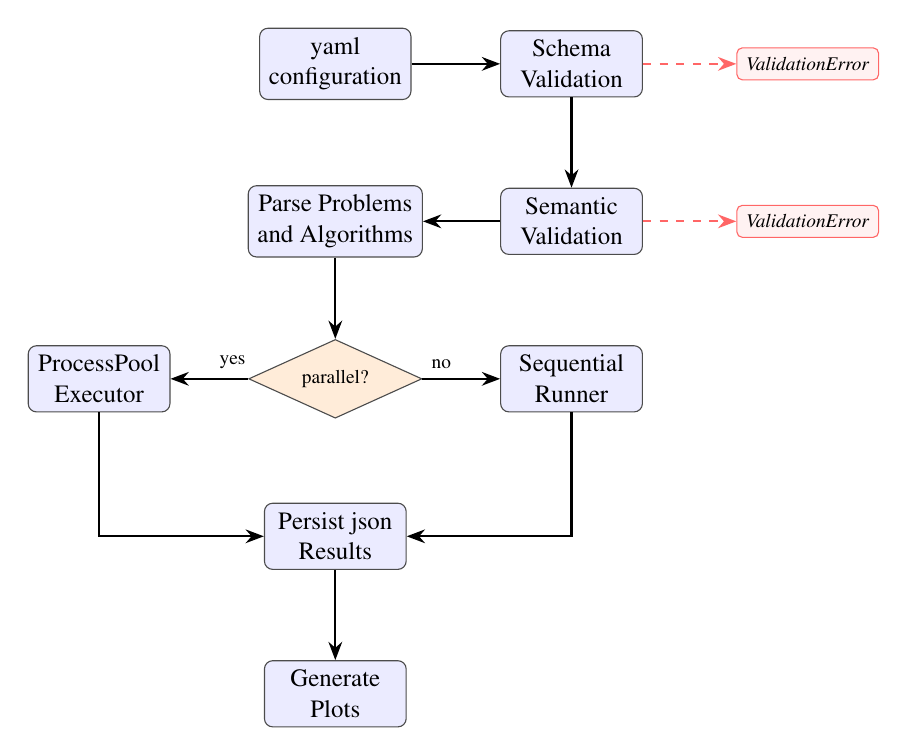
\begin{tikzpicture}[
      node distance = 2cm and 3cm,
      on grid,
      box/.style = {
        rectangle, rounded corners=3pt, draw=black!70,
        fill=blue!8, minimum width=1.8cm,
        minimum height=0.8cm, font=\small, align=center
      },
      decision/.style = {
        diamond, draw=black!70, fill=orange!15,
        minimum width=2.2cm, minimum height=1.0cm,
        font=\scriptsize, align=center, aspect=2
      },
      errbox/.style = {
        rectangle, draw=red!60, fill=red!5, rounded corners=2pt,
        font=\scriptsize, align=center
      },
      arrow/.style = {->, >=Stealth, thick},
      darrow/.style = {->, >=Stealth, thick, dashed, red!60}
    ]

    \node[box]   (yaml)  {\acrshort{yaml}\\configuration};
    \node[box,   right=of yaml]  (schema) {Schema\\Validation};
    \node[box,   below=of schema] (sem)  {Semantic\\Validation};
    \node[box,   left=of sem]  (parse) {Parse Problems\\and Algorithms};

    \node[decision, below=of parse] (par) {parallel?};

    \node[box, right=3.0cm of par] (seq) {Sequential\\Runner};
    \node[box, left=3.0cm of par] (pool) {ProcessPool\\Executor};

    \node[box, below=of par] (persist) {Persist \acrshort{json}\\Results};
    \node[box, below=of persist] (plots) {Generate\\Plots};

    \node[errbox, right=of schema] (e1) {\textit{ValidationError}};
    \node[errbox, right=of sem]  (e2) {\textit{ValidationError}};

    \draw[arrow] (yaml)  -- (schema);
    \draw[arrow] (schema) -- (sem);
    \draw[arrow] (sem)  -- (parse);
    \draw[arrow] (parse) -- (par);

    \draw[arrow] (par) -- node[above left] {\scriptsize no} (seq);
    \draw[arrow] (par) -- node[above right] {\scriptsize yes} (pool);

    \draw[arrow] (seq) |- (persist);
    \draw[arrow] (pool) |- (persist);

    \draw[arrow] (persist) -- (plots);

    \draw[darrow] (schema) -- (e1);
    \draw[darrow] (sem)  -- (e2);

  \end{tikzpicture}
  \caption[Configuration parse pipeline]{Validation and job dispatch
    pipeline. \acrshort{yaml} configuration files are
    validated structurally via \acrshort{json} Schema and then
    semantically against
    class registries before execution begins. Any validation failure
    raises a \texttt{ValidationError} and halts the pipeline before
  computation begins.}
  \label{fig:dispatch-pipeline}
\end{figure}

\subsubsection{Raw Output \acrshort{json} files}
The output \acrshort{json} files are \textit{compacted} by replacing
redundant stylistic whitespaces and newlines with other separators.
This reduced the raw file sizes by up to 50\%.
\acrshort{json} files were preferred for storing the raw files since
it included \textit{mixed} data, including metadata, general
statistics for each run, along with the trajectories.
A `NoSQL' (key-value) database was considered but not used since the
experiments were relatively small scale.

\subsubsection{UML Diagram}
% Diagram
Figure~\ref{fig:uml} presents the core class structure of the
framework. Abstract base classes \texttt{Problem} and
\texttt{Algorithm} define the shared interface enforced across all concrete
implementations. Concrete subclasses are registered by string key and
resolved at runtime. \texttt{ExperimentRunner} orchestrates individual runs
and delegates result persistence, while the \texttt{CoolingSchedule} protocol
is resolved from \acrshort{yaml} at parse time via a \textit{registry}.

\begin{figure}[H]
  \centering
  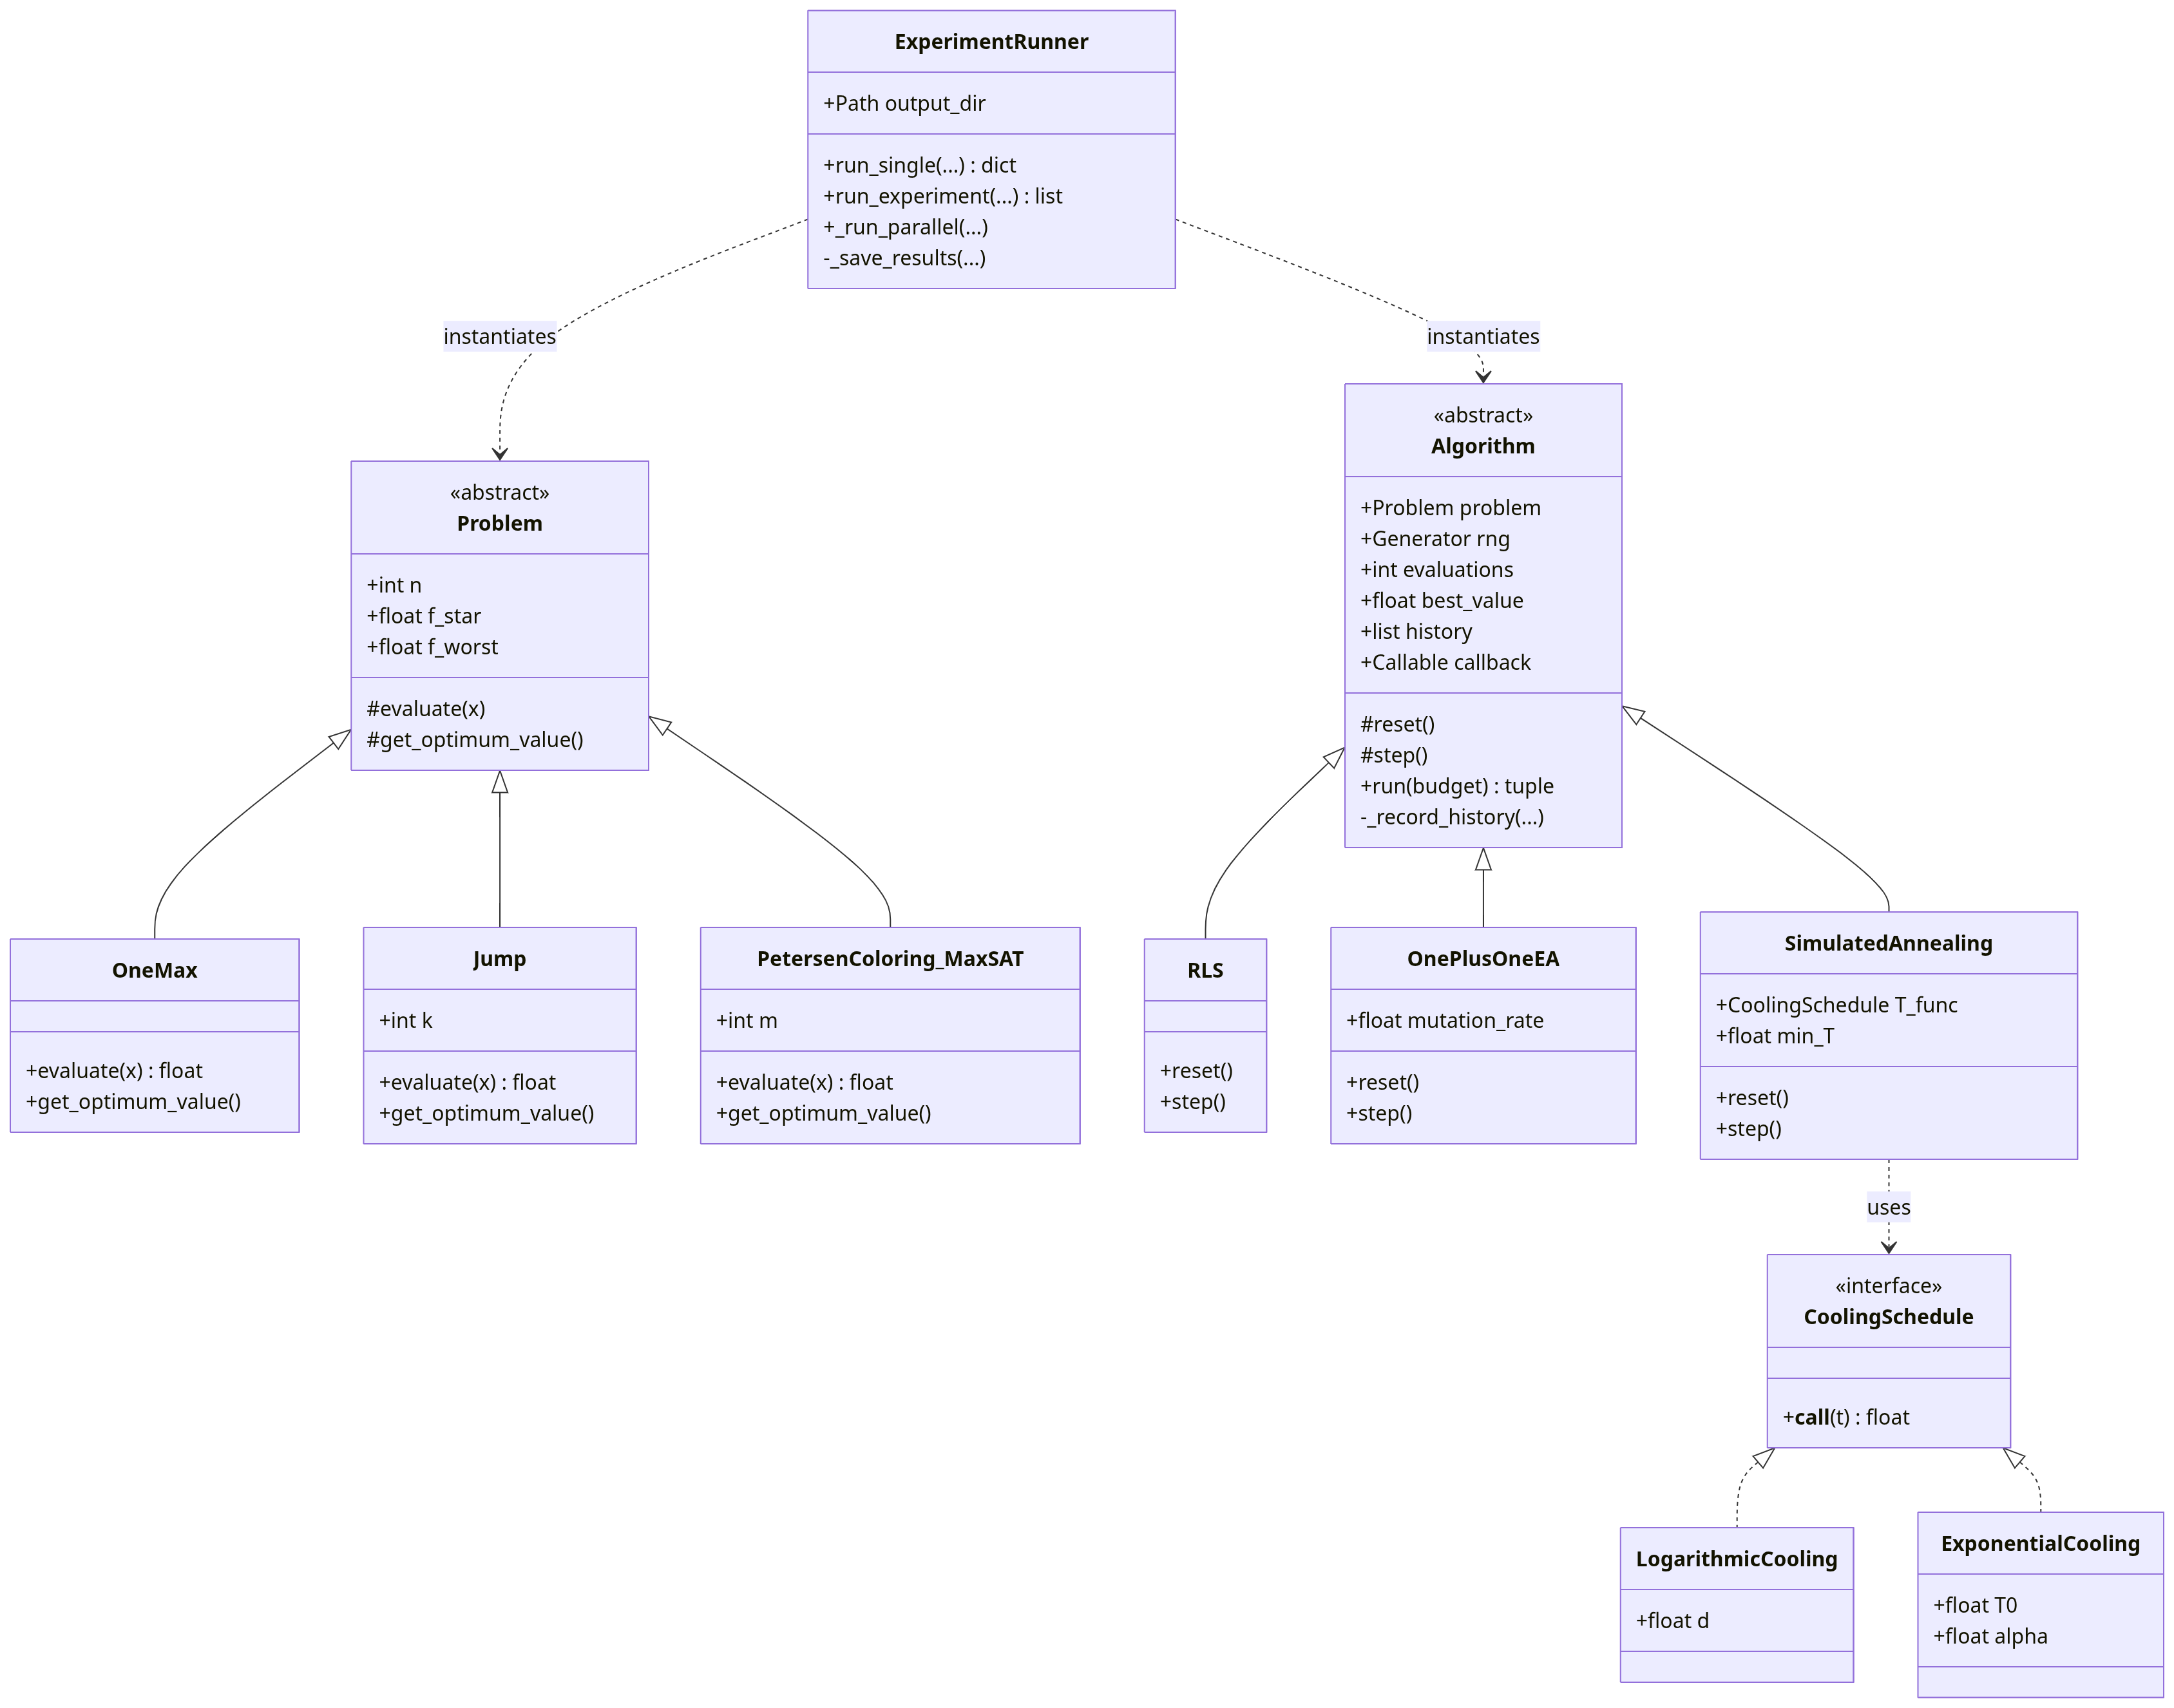
\includegraphics[width=\linewidth]{uml.png}
  \caption[UML class diagram]{Simplified UML class diagram of the
    \texttt{regret} framework.
    Solid triangle arrows ($\triangleright$) denote inheritance;
    dashed arrows denote dependency or instantiation.
    Hashes `\#' indicate abstract declarations.
    Several concrete subclasses (e.g.\ \texttt{MuPlusLambdaEA},
      \texttt{\acrlong{rlse}}, \texttt{NKLandscape},
  \texttt{LinearCooling}) are omitted for clarity.}
  \label{fig:uml}
\end{figure}

\subsection{Limitations}
% Does not support multi-objective optimization, continuous
% optimization, limited to binary strings.
The framework is currently constrained to \textbf{binary search spaces}
$\{0,1\}^n$; continuous and non-binary integer decision domains are not
supported.
\textbf{Multi-objective optimization} is not implemented. The NK landscape
optimum computation uses exhaustive search, restricting its practical use to
$n \leq 20$. Runtime profile analysis assumes integer-valued or explicitly
discretized fitness levels for the exact tail-sum identity:
\[
  \mathbb{E}[\mathrm{CR}(T)]
  \;=\;
  \sum_{v=1}^{f^{*}}\sum_{t'=1}^{T}
  \bigl[1 - P(\tau_v \leq t')\bigr];
\]
real-valued fitness functions (e.g.\ \texttt{NK-Landscape}) require
discretization and therefore yield approximate runtime-profile results.

% Considering addition to the next chapter.
\subsection{Result Interpretations}
\label{subsec:resint}
% % Max 200 words
% % Describe the output file structure, explaining the organisation.

All experiment output is written under a structured directory hierarchy.
Raw \acrshort{json} result files are stored at:

\texttt{results/raw/<suite>/<problem>/<algorithm>/n<N>/b<B>.json}

\noindent where \texttt{<suite>}, \texttt{<problem>}, and
\texttt{<algorithm>} are
normalized display names, \texttt{N}~is the problem dimension, and \texttt{B}
is the evaluation budget. Each file contains three top-level keys:
\texttt{metadata} (algorithm, problem class, dimension, budget, run count,
mode, and timestamp), \texttt{statistics} (mean, median, standard deviation,
quartiles, and probability of optimum across all runs), and \texttt{results}
(an ordered list of per-run dictionaries each containing regret, best value,
  optimality flag, evaluation count, seed, and the complete trajectory
(in \texttt{full} mode)).

Generated figures are written under \texttt{results/figures/} following an
analogous hierarchy:

\texttt{results/figures/<suite>/<problem>/n<N>/<subdir>/<filename>.pdf}

\noindent Plot subdirectories are configurable via
\texttt{layout.structure} in the YAML
configuration; the defaults are \texttt{aggregate/} for cross-budget plots,
\texttt{history/} for trajectory and regret time-series plots, and
\texttt{distributions/} for budget-specific box-plots and performance profiles.
Runtime profile plots are written to a \texttt{profiles/} subdirectory within
the raw results tree. All figures are saved as \acrshort{pdf} at
300\,\acrshort{dpi}.
Table~\ref{tab:output-structure} summarizes the full output organization.

\small
\begin{longtable}{p{0.55\linewidth}p{0.45\linewidth}}
  \hline
  \textbf{Path pattern} & \textbf{Contents} \\
  \hline
  \multicolumn{2}{l}{\textit{Raw data (JSON)}} \\
  \hline
  \small\texttt{results/raw/\newline<suite>/<prob>/<algo>/n<N>/b<B>.json}
  & Per-budget result file: metadata, aggregate statistics, per-run regrets,
  and (in \texttt{full} mode) full evaluation trajectories. \\[4pt]
  \small\texttt{results/raw/<suite>/<prob>/}\newline\texttt{profiles/n<N>/cr\_profile\_data\_<algo>.csv}
  & Runtime profile CSV; columns: \texttt{evaluation},
  \texttt{expected\_cumulative\_regret},
  \texttt{mean\_cumulative\_regret}. \\
  \hline
  \multicolumn{2}{l}{\textit{Figures (\acrshort{pdf}, 300\,DPI)}} \\
  \hline
  \texttt{.../n<N>/aggregate/}
  & Cross-budget plots: regret curves, convergence probability,
  comparison heatmap. \\[4pt]
  \texttt{.../n<N>/history/}
  & Trajectory plots: best/current value, instantaneous and cumulative
  regret, \acrfull{ttfo} distribution. \\[4pt]
  \texttt{.../n<N>/distributions/}
  & Budget-specific plots: regret box-plots and performance profiles. \\[4pt]
  \texttt{.../n<N>/profiles/}
  & Runtime profile plots: inverse profile surface/curves,
  $\mathbb{E}[\mathrm{CR}(T)]$ verification.
  Requires \texttt{suite.profile: true}. \\
  \hline
  \caption[Experiment output organization]{Output file organization
    for a representative experiment.
    ``Normalization'' replaces spaces, parentheses, and special characters
  with underscores or removes them.}
  \label{tab:output-structure}
\end{longtable}

\small
\begin{longtable}{p{4cm}p{8cm}p{2cm}}
  \hline
  \textbf{Plot} & \textbf{Output filename pattern - \texttt{\acrshort{pdf}}
  format} & \textbf{Profile required} \\
  \hline
  Regret curves            & \texttt{regret\_curves}
  & No \\
  Convergence probability  & \texttt{convergence\_probability}
  & No \\
  Comparison heatmap       & \texttt{comparison\_heatmap}
  & No \\
  Regret box-plots          & \texttt{regret\_boxplot\_b\{budget\}}
  & No \\
  Performance profile      &
  \texttt{performance\_profile\_b\{budget\}}    & No \\
  History (best-so-far)    & \texttt{history\_best}
  & No \\
  Instantaneous regret     &
  \texttt{history\_regret\_instantaneous}       & No \\
  Cumulative regret        & \texttt{history\_regret\_cumulative}
  & No \\
  \acrshort{ttfo} distribution        &
  \texttt{history\_ttfo\_markers}               & No \\
  Runtime profile surface  &
  \texttt{inverse\_runtime\_profile\_surface\_\{alg\}} & Yes \\
  Runtime profile curves   &
  \texttt{inverse\_runtime\_profile\_curves}   & Yes \\
  CR profile verification  & \texttt{cr\_profile\_verification}
  & Yes \\
  \hline
  \caption[Generated experiment plot types]{Plot types generated
    across experiments. ``Profile required'' denotes
  plots that require \texttt{suite.profile:~true}}
  \label{tab:plot-types}
\end{longtable}

\section{Testing strategy}
% Mention TDD, Red-Green Testing, selective coverage (weighted)
\begin{wrapfigure}{r}{0.5\textwidth} %this figure will be at the right
  \centering
  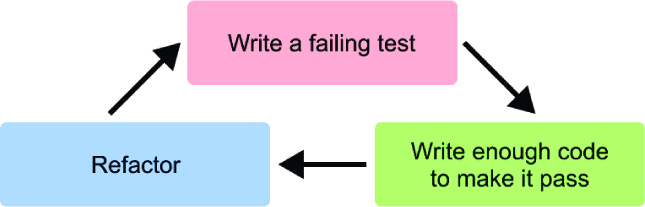
\includegraphics[width=0.5\textwidth]{red-green-refactor.png}
  \caption[Red--Green--Refactor \acrshort{tdd}
  technique]{Red--Green--Refactor \acrshort{tdd} technique. Start by
    writing a failing test (the red step). Next, write code that is
    just enough to make the written test pass (the green step).
    Finally, as the regularities and properties of the problem space
    are understood, refactors can be implemented that keeps the code
    clean (the blue step). The refactor step is safe since it will
  always be backed up by tests.~\cite{calais2023test}}
\end{wrapfigure}
The test suite follows a \acrfull{tdd} discipline
using a red--green--refactor workflow: tests were written prior to or alongside
implementation and serve as executable
specifications~\cite{agha2023test,calais2023test}. Coverage is measured
using the \texttt{coverage}~\cite{coverage} package with branch
tracking enabled, and a
minimum threshold of \textbf{50\% branch coverage} is enforced in
\acrfull{ci} via GitHub Actions. Coverage is also computed across
Python~3.12, 3.13, and 3.14 in \acrfull{ci} for redundancy and
support (the project must be compatible for \texttt{python} $\geq$ 3.12).

Test organization follows a selective weighting strategy: core algorithmic
components (\texttt{test\_algorithms.py}, \texttt{test\_metrics.py},
\texttt{test\_problems.py}) and integration paths
(\texttt{test\_integration.py}) receive dense coverage, while infrastructure
components such as CLI wiring and plot dispatch are covered at a coarser
granularity.

\section{Project Dependencies}
The project is built with \texttt{hatchling}~\cite{hatchling} and managed
with \texttt{uv}~\cite{uv}, a Rust-based package and environment manager that
replaces the Python standard \texttt{pip}/\texttt{venv}.
Runtime installation: \texttt{uv sync}; development installation:
\texttt{uv sync -{}-group dev}.

\small
\begin{longtable}{p{3cm}p{3cm}p{8cm}}
  \hline
  \textbf{Package} & \textbf{Min.\ version} & \textbf{Purpose} \\
  \hline
  \multicolumn{3}{l}{\textit{Scientific computing}} \\
  \hline
  \texttt{numpy}~\cite{numpy}      & 2.4.3  & Array operations,
  random number generation \\
  \texttt{scipy}~\cite{scipy}      & 1.16.3 & Statistics, drift
  computations, profile integrals \\
  \texttt{pandas}~\cite{pandas}    & 2.3.3  & Results aggregation,
  tabulation, CSV export \\
  \hline
  \multicolumn{3}{l}{\textit{Visualisation}} \\
  \hline
  \texttt{matplotlib}~\cite{matplotlib} & 3.10.8 & All static plot
  generation \\
  \texttt{ipympl}                       & 0.10.0 & Interactive
  Matplotlib in notebooks \\
  \texttt{networkx}~\cite{networkx}& 3.6.1  & Graph problem
  instances (e.g.\ Petersen colouring) \\
  \hline
  \multicolumn{3}{l}{\textit{Configuration and \acrshort{cli}}} \\
  \hline
  \texttt{pyyaml}~\cite{pyyaml}      & 6.0.3  & Experiment
  configuration parsing \\
  \texttt{jsonschema}~\cite{jsonschema}  & 4.26.0 & \acrshort{yaml}
  schema validation \\
  \texttt{typer}~\cite{typer}       & 0.24.1 &
  \texttt{run\_experiment} \acrshort{cli} \\
  \texttt{tqdm}~\cite{tqdm}        & 4.67.1 & Progress bars for
  parallel runs \\
  \hline
  \multicolumn{3}{l}{\textit{Notebook and interactive demonstration}} \\
  \hline
  \texttt{jupyter}~\cite{jupyter}     & 1.1.1  & Notebook server \\
  \texttt{ipykernel}   & 7.2.0  & Jupyter kernel support \\
  \texttt{ipywidgets}  & 8.1.8  & Notebook UI widgets \\
  \hline
  \multicolumn{3}{l}{\textit{Development --- linting (optional)}} \\
  \hline
  \texttt{ruff}~\cite{ruff} & --- & Fast Rust-based linter and
  formatter (E, W, F, I, B, UP rules) \\
  \hline
  \multicolumn{3}{l}{\textit{Development --- testing (optional)}} \\
  \hline
  \texttt{pytest}~\cite{pytest}    & --- & Unit and integration test runner \\
  \texttt{coverage}~\cite{coverage}  & --- & Branch coverage
  reporting ($\geq$50\% enforced) \\
  \texttt{tabulate}  & --- & Tabular output in test fixtures \\
  \hline
  \multicolumn{3}{l}{\textit{Development --- type checking (optional)}} \\
  \hline
  \texttt{ty}~\cite{ty} & --- & Rust-based static type checker (Astral) \\
  \hline
  \multicolumn{3}{l}{\textit{Development --- documentation (optional)}} \\
  \hline
  \texttt{zensical}              & --- & Documentation site generator \\
  \texttt{mkdocstrings-python}   & --- & Auto-generated API
  reference from docstrings \\
  \hline
  \caption[Table of software prerequisites]{%
    Package dependencies for the \texttt{regret} framework (Python~$\geq$~3.12).
  }
  \label{tab:dependencies}
\end{longtable}

% Word count aim                0700-0800

% \chapter{Experiments}
% \label{cha:exper}
% 
% \section{Experiment Structure}
% 
% \section{Exploratory Analysis of Regret \& Runtime}
% \subsection{Experiment 1}
% \subsection{Experiment 2}
% \subsection{Experiment 3}
% \subsection{Experiment 4}
% 
% 
% \section{Expected Cumulative Regret and Runtime Profiles}
% % TODO: Clarify structure of such experiments
% % Gist: Math motiv -> setup -> collection of results (mentioned for both the experiment types in next chapter)
% \subsection{}

\chapter{Experiments}
\label{cha:exper}
 
\section{Experiment Structure}
\label{sec:exper:structure}
 
All experiments share a common infrastructure defined in the YAML configuration
files under \texttt{configs/experiments/} !TODO: Cite appendices!. 
Each configuration specifies four top-level blocks: \texttt{suite} 
(global settings), \texttt{problems} (benchmark functions), 
\texttt{algorithms} (optimisers), and \texttt{plotting} (output).
 
\subsection{Repetitions and budget}
Every algorithm--problem pair is evaluated over $R$ independent runs (typically
25--100, chosen to keep Monte-Carlo variance !CITE! in $\mathbb{E}[\text{CR}(T)]$
negligible), each run consuming up to a fixed evaluation budget $T_{\max}$
drawn from a per-suite budget list. A separate \texttt{budget\_for\_plots}
value, calibrated to approximately twice the expected time-to-first-optimum
($\mathbb{E}[\text{TTFO}]$) for the hardest algorithm on each problem, governs
the time horizon displayed in trajectory plots.
 
\subsection{Execution mode}
All suites run in \texttt{full} mode with parallelism enabled. 
The \texttt{full} supports recording the evaluation time-series. 
It was trivially toggled for these experiments.
Suites that compute inverse runtime profiles additionally set
\texttt{profile:~true}, which enables trajectory-level data collection required
for the tail-sum verification and runtime-profile plots.
 
% \subsection{Output}
% Raw results are written as \acrshort{json} under \texttt{results/raw/}, organized by suite,
% problem, and algorithm. Figures are written under \texttt{results/figures/}
% with a per-problem, per-size subdirectory structure~\ref{subsec:resint}. These results can be regenerated 
% with for each configuration of the experiment via the \acrshort{cli}.
% Plot types are described in Table~\ref{tab:plot-types}. (See Subsection~\ref{subsec:resint})

\subsection{Visualisation and Table Strategy}

The output of each suite consists of plots and summary tables generated from
the stored \acrshort{json} results. Plot types fall into four groups:
aggregate, budget-specific distribution, trajectory, and runtime profile.

\paragraph{Aggregate plots.}
Three plots pool results across all budgets in the suite budget list.
\emph{Mean simple-regret curves} (\texttt{regret\_curves}) plot
$\widehat{\mathbb{E}}[f^{*}-f(x_{\text{best}})]$ against evaluation budget
on a log--log axis with one shaded curve per algorithm; a steeper slope or
earlier crossover indicates a faster-decaying algorithm. When all algorithms
converge fully within the budget range this plot loses resolution, in which
case the \emph{convergence probability} plot (\texttt{convergence\_probability})
is more informative: it shows the fraction of runs reaching regret below
$10^{-9}$, separating algorithms by the budget at which they first converge
reliably. The \emph{comparison heatmap} (\texttt{comparison\_heatmap})
encodes $\log_{10}(\text{mean regret})$ as a colour over all
algorithm--budget cells, providing a compact global overview but at lower
precision than the regret curves.

\paragraph{Budget-specific distribution plots.}
These are generated once per problem at the budget specified by
\texttt{budget\_for\_plots}. \emph{Regret boxplots}
(\texttt{regret\_boxplots}) show the distribution of simple regret across
runs with individual points overlaid, exposing skewness and run-to-run
variability that means cannot: two algorithms can share the same mean while
one converges reliably on most runs and fails completely on a few.
\emph{Performance profiles} (\texttt{performance\_profile}) show the
empirical CDF of simple regret on a log-scaled axis; a curve that rises
steeply at low regret values indicates reliable near-optimal convergence,
whereas a gradual rise indicates high variability. Both plots support optional
pairwise statistical annotation (Mann--Whitney U and Cohen's $d$ against a
reference algorithm).

\paragraph{Trajectory plots.}
All trajectory plots are averaged across runs at \texttt{budget\_for\_plots},
with a standard-error band and optional TTFO markers at the mean
time-to-first-optimum. The suite produces several complementary variants.

The \emph{best-value history} (\texttt{history\_best}) plots the
monotonically non-decreasing incumbent fitness against evaluation time,
providing an absolute fitness view with $f^{*}$ as a horizontal reference.

\emph{Instantaneous regret} is produced in two variants.
With \texttt{track\_incumbent: false} (\texttt{regret\_instantaneous}),
it is the gap between $f^{*}$ and the solution evaluated at each step,
which fluctuates whenever an algorithm accepts a worsening move.
With \texttt{track\_incumbent: true} (\texttt{regret\_instantaneous\_best}),
it is the gap from $f^{*}$ to the incumbent, which is monotonically
non-increasing and equivalent to simple regret measured at each $t$.
For hill-climbing algorithms (RLS, $(1+1)$-EA) the two variants coincide
because no worsening moves are accepted; for SA and RLSExploration they
diverge during phases of active exploration. Both are plotted on a log-$y$
axis. A flat non-zero floor in the incumbent variant on this axis is the
primary diagnostic signature of saturation at a local optimum.

\emph{Cumulative regret} (\texttt{regret\_cumulative} and
\texttt{regret\_cumulative\_best}) is the integral of the corresponding
instantaneous regret series over time. It penalises slow convergence: an
algorithm that reaches $f^{*}$ late has accumulated all preceding regret
regardless of final solution quality. The slope of the cumulative regret curve
during the trapped phase grows linearly with time and is the key signal for
barrier-crossing suites (05, 06, 09, 10); this slope is suppressed on a
log axis, so cumulative regret is plotted on a linear $y$-axis throughout.

The \emph{TTFO distribution} (\texttt{ttfo\_distribution}) plots individual
run-level times-to-first-optimum as jittered points per algorithm. This plot
is conditioned on convergence: runs that did not reach the optimum contribute
no point, so when $P(\text{opt}) \approx 0$ across the suite the scatter is
sparse and adds little beyond the convergence probability plot.

\paragraph{Runtime profile plots.}
These require \texttt{suite.profile:~true} and are produced only in suites
03, 08, and 12. The inverse runtime profile
$P(\tau_v \leq T)$---the probability that fitness level $v$ was first reached
by evaluation $T$---is the common basis.

The \emph{profile surface} (\texttt{inverse\_runtime\_profile\_surface})
plots this probability as a heat map over $(T, v)$ for each algorithm
separately, with iso-probability contours overlaid. A front that stalls at
some $v_{\text{local}} < f^{*}$ regardless of additional budget identifies
the saturation level of the algorithm on that landscape.
The \emph{profile curves} (\texttt{inverse\_runtime\_profile\_curves}) plot
$P(\tau_v \leq T)$ versus $T$ at four selected fitness levels
($f^{*} \times \{0.25, 0.5, 0.75, 0.95\}$), overlaying all algorithms on
the same panel for direct comparison.

The \emph{profile verification} plot (\texttt{cr\_profile\_verification}),
enabled only in suite 08, overlays two independent estimates of
$\mathbb{E}[\text{CR}(T)]$: the empirical mean across runs, and the value
derived via the tail-sum identity from the inverse profile. For integer-valued
unit-increment fitness functions the identity is exact and any gap indicates a
computational error; for the continuous-valued NK landscape (suite 12) a minor
gap reflects finite-grid discretisation and not a bug.

\paragraph{Summary tables.}
Tables are exported per-suite in \LaTeX, CSV, or Markdown.
A \emph{per-problem table} is produced at each budget for each problem, with
one row per algorithm reporting mean, median, standard deviation, interquartile
range, a 95\% bootstrap confidence interval, $P(\text{opt})$, and run count,
sorted by ascending mean regret. The mean--median gap is informative when
distributions are skewed by a minority of non-converging runs.
An \emph{aggregate cross-problem table} summarises each algorithm's
across-problem mean regret, mean $P(\text{opt})$, and the count of problems
on which it achieved the lowest mean regret among all algorithms in the suite.


 
\subsection{Experiment numbering}
Suites are numbered 01--14. Suites 01--02 establish the baseline algorithm-family
comparison. Suites 03--07 and 09--14 form the exploratory analyses. Suite~08 is
a dedicated verification suite for the tail-sum identity.
Suites 03 and 12 additionally enable runtime profiling to study saturation
phenomena on NK landscapes alongside the verification suite.

\section{Runtime Profiles}


\subsection{Motivation}

The predominant performance measure in the runtime analysis of \acrshort{ea}s
is the \textit{expected optimization time}: the expected number of function evaluations
until an optimal solution is queried for the first
time~\cite{droste2002analysis,doerr2020theory}. While this measure has proved immensely
useful for ranking algorithms and establishing complexity hierarchies, it carries a
significant limitation for practice. In almost all realistic settings, a user cannot
detect when the algorithm has found an optimum. Even if this were possible, the
number of evaluations required to guarantee optimality may be prohibitively
large~\cite{pinto2018practice}. What the practitioner actually observes is the evolution
of solution quality over the \emph{entire} course of the run.

Two complementary frameworks have been proposed to address this limitation. The first,
from Jansen and Zarges~\cite{jansen2014fixed}, adopts a \textit{fixed-budget
perspective}: fix the evaluation budget $T$ in advance and characterize the expected
quality of the best solution found within that budget. The second, introduced by Pinto
and Doerr~\cite{pinto2018practice}, proposes \textit{runtime profiles}: rather than
reporting only the expected time to reach the global optimum, report the expected time
to reach each intermediate fitness level. These two views are orthogonal; one fixes
time and studies expected solution quality, the other fixes solution quality and studies
expected time. However, both provide richer information than the single expected
optimization time, as supported by Pinto and Doerr:
\begin{displayquote}
Our intention is rather to highlight to researchers working on theoretical aspects in
evolutionary computation that, beyond being possibly more relevant for practitioners,
explicitly reporting runtime profiles can give quite interesting insights into the
performance of \acrshort{ea}s.
{(\cite{pinto2018practice}, p.~19)}
\end{displayquote}

\subsection{Fixed-Budget Analysis}

In \textit{fixed-budget analysis}~\cite{jansen2014fixed}, the evaluation budget $T$ is
fixed in advance and the quantity of interest is the distribution of solution quality
achieved within that budget. Formally, let $f^{*}_T(\mathcal{A})$ denote the best
objective value achieved by algorithm $\mathcal{A}$ within $T$ evaluations on objective
$f$. Fixed-budget analysis characterizes $\mathbb{E}[f^{*}_T(\mathcal{A})]$ as a
function of $T$~\cite{jansen2014fixed}.

Fixed-budget analysis is particularly relevant in practice, where resources are finite
and an algorithm must return the best solution found when the budget is exhausted,
regardless of whether the global optimum has been identified~\cite{jansen2014fixed}. It
connects naturally to the simple regret framework: minimizing simple regret over a
fixed budget $T$ is equivalent to maximizing $\mathbb{E}[f^*_T(\mathcal{A})]$. Comparing
two algorithms under a fixed budget may yield different conclusions than comparing their
expected runtimes, since an algorithm with a larger expected optimization time may still
produce better intermediate solutions within a given budget~\cite{jansen2014fixed}.

\subsection{Variants}

\subsubsection{Expectation-Based Runtime Profiles}

Pinto and Doerr~\cite{pinto2018practice} propose that runtime results for evolutionary
algorithms should include not only the expected time to reach the global optimum but
also the expected time needed to reach each intermediate fitness level. Concretely, for
a fitness function $f : \{0,1\}^n \to \mathbb{R}$ with global optimum $f^* = \max_x
f(x)$, and for each target level $v$, the \textit{first hitting time} of level $v$ is
\begin{equation}
    \tau_v \;:=\; \min\bigl\{t \in \mathbb{N} : f(x_t) \geq v\bigr\},
\end{equation}
where $x_1, x_2, \ldots$ is the sequence of query points produced by the
algorithm~\cite{droste2002analysis}. The \textit{expectation-based runtime profile}
of an algorithm is the collection of expected first hitting times
$\bigl(\mathbb{E}[\tau_v]\bigr)_{v}$ across all relevant target
levels~\cite{pinto2018practice}.

When canonical fitness levels exist, such as for \textsc{OneMax} or
\textsc{LeadingOnes}, these provide natural targets; for other functions, intermediate
values identified during the analysis or obtained by linear interpolation of the minimal
and maximal fitness values may be used~\cite{pinto2018practice}. Crucially, Pinto and
Doerr emphasize that this framework does not require new algorithms or new proof
techniques, all bounds can be derived from existing runtime results and are often
already implicit in the proofs~\cite{pinto2018practice}. The proposal is therefore one
of \emph{presentation}: reporting richer, more informative performance summaries that
better reflect the anytime behavior of an algorithm.

The practical value of this richer view is illustrated by the behavior of (1+1)~\acrshort{ea}
variants on \textsc{LeadingOnes}: reporting only the expected optimization time suggests
RLS is superior, yet the runtime profile reveals that
(1+1)~EA$_{>0}$ (see !TODO: ref (1+1)-EA\_{>=0} variant!)
reaches all intermediate fitness levels $i \leq 7{,}980$ faster than RLS for problem
size $n = 10{,}000$, with RLS only pulling ahead in the final portion of the
run~\cite{pinto2018practice}. Such crossover behavior is invisible to the single
expected optimization time and is directly relevant to the design of adaptive parameter
and operator selection schemes~\cite{pinto2018practice}.

\subsubsection{Distributional Runtime Profiles}

The expectation-based runtime profile of~\cite{pinto2018practice} summarizes the
distribution of $\tau_v$ by its mean. A finer characterization, and the appropriate
quantity for connecting runtime profiles to regret-based measures, is the
\textit{distributional runtime profile}
\begin{equation}
    \mathcal{P}(v, t) \;:=\; \mathbb{P}(\tau_v > t),
\end{equation}
which records, for each target level $v$ and time step $t$, the probability that level
$v$ has not yet been reached by time $t$. The expectation-based profile is recovered by
the standard tail-sum formula for non-negative integer-valued random
variables~\cite{doerr2020theory}:
\begin{equation}
    \label{eqn:dist-runtime-rel}
    \mathbb{E}[\tau_v] \;=\; \sum_{t=0}^{\infty} \mathbb{P}(\tau_v > t).
\end{equation}
The distributional profile is the more primitive object from which expectation-based
statements follow, and it constitutes the link between runtime profiles and the
regret-based framework developed below.

\begin{remark}[Naming convention]
\label{rem:profile-naming}
The term \emph{runtime profile} appears in two distinct senses in the literature and in
this work. Pinto and Doerr~\cite{pinto2018practice} use it to denote the
\emph{expectation-based} runtime profile $\bigl(\mathbb{E}[\tau_v]\bigr)_v$, which
summarizes per-level performance by expected hitting times. The present work additionally
employs the strictly finer \emph{distributional} runtime profile $\mathcal{P}(v,t) =
\mathbb{P}(\tau_v > t)$, from which the expectation-based profile is recovered via the
tail-sum formula (Equation \ref{eqn:dist-runtime-rel}). To avoid ambiguity, the two notions are referred to explicitly whenever
both are in scope. Hereafter, and in all practical experimentation in this report,
\emph{runtime profile} refers to the distributional variant $\mathcal{P}(v,t)$ unless
otherwise stated.
\end{remark}

\subsection{Connection to Cumulative Regret}
\label{subsec:regret-profiles}

One of the discussions suggested by Pinto and Doerr in their \textit{Future Works}
section is highlighted:
\begin{displayquote}
    We feel that there is a need for combined measures that are capable of describing
    the anytime behavior of an EA[`Evolutionary Algorithms']. Regret-based measure as
    used in machine learning could be a key here, but we haven't been able so far to
    identify a fully satisfying measure.
    {(\cite{pinto2018practice}, p.~22)}
\end{displayquote}
As far as we know, establishing such a relationship remains an open question. This consolidated the following proposal for exploring the established concepts of \textit{\acrfull{cr}} and \textit{Runtime Profiles}.

The relationship between runtime profiles and \acrshort{cr} can be made precise
through a formal setup. A randomized black-box algorithm produces an adaptive sequence
of query points $x_1, x_2, \ldots \in \{0,1\}^n$. Define the
\textit{best-so-far process}
\[
    B(t) \;:=\; \max_{s \leq t} f(x_s),
\]
which records the best objective value seen up to time $t$. Since $B(t)$ is
non-decreasing in $t$, the event $\{B(t) < v\}$ is equivalent to $\{\tau_v > t\}$
(the level $v$ has not yet been hit). The \textit{\acrshort{cr}} with respect to the
global optimum $f^*$ over a budget of $T$ evaluations is~\cite{cesa2006prediction}
\[
    \mathrm{CR}(T) \;:=\; \sum_{t=1}^{T} \bigl(f^* - B(t)\bigr).
\]

The proof of the main theorem relies on two elementary lemmas.

\begin{lemma}[Tail-sum representation for the gap]
\label{lem:tailsum}
For any integer $b$ with $0 \le b \le f^*$,
\[
    f^* - b \;=\; \sum_{v=1}^{f^*} \mathbf{1}[b < v].
\]
\end{lemma}

\begin{proof}
The right-hand side counts the integers $v \in \{1,\ldots,f^*\}$ that strictly exceed
$b$, namely the set $\{b+1,\ldots,f^*\}$, which has cardinality $f^* - b$.
\end{proof}

\begin{lemma}[Indicator equivalence]
\label{lem:indicator}
For all $v \in \{1, \ldots, f^*\}$ and $t \in \mathbb{N}$,
\[
    \mathbf{1}[B(t) < v] \;=\; \mathbf{1}[\tau_v > t].
\]
\end{lemma}

\begin{proof}
Since $B(t)$ is non-decreasing in $t$, the event $\{B(t) \ge v\}$ is equivalent to
$\{\tau_v \le t\}$. Taking complements gives $\{B(t) < v\} = \{\tau_v > t\}$, so the
two indicators agree on every sample path.
\end{proof}

The following identity connects \textit{expected} cumulative regret to the distributional
runtime profile.

\begin{theorem}[Tail-Sum Regret Representation]
\label{thm:regret-profile}
For any randomized black-box algorithm operating on $f$ with finite budget
$T \in \mathbb{N}$,
\[
    \mathbb{E}[\mathrm{CR}(T)]
    \;=\;
    \sum_{v=1}^{f^*} \sum_{t=1}^{T} \mathbb{P}(\tau_v > t).
\]
\end{theorem}

\begin{proof}
For each $t$, Lemma~\ref{lem:tailsum} applied to $b = B(t)$ gives
\[
    f^* - B(t) \;=\; \sum_{v=1}^{f^*} \mathbf{1}[B(t) < v].
\]
Summing over $t = 1, \ldots, T$ yields
\[
    \mathrm{CR}(T)
    \;=\; \sum_{t=1}^{T}\bigl(f^* - B(t)\bigr)
    \;=\; \sum_{t=1}^{T} \sum_{v=1}^{f^*} \mathbf{1}[B(t) < v].
\]
By Lemma~\ref{lem:indicator}, $\mathbf{1}[B(t) < v] = \mathbf{1}[\tau_v > t]$ on every
sample path, so
\[
    \mathrm{CR}(T) \;=\; \sum_{t=1}^{T} \sum_{v=1}^{f^*} \mathbf{1}[\tau_v > t].
\]
Taking expectations and applying linearity of expectation together with
$\mathbb{E}[\mathbf{1}[\tau_v > t]] = \mathbb{P}(\tau_v > t)$ gives
\[
    \mathbb{E}[\mathrm{CR}(T)]
    \;=\; \sum_{t=1}^{T} \sum_{v=1}^{f^*} \mathbb{P}(\tau_v > t).
\]
Since both sums are finite, their order may be exchanged, yielding the stated result.
\end{proof}

Theorem~\ref{thm:regret-profile} expresses expected cumulative regret as a double sum
of the distributional runtime profile: $\mathbb{E}[\mathrm{CR}(T)]$ is the total
expected time the algorithm spends below each fitness level $v$, summed over all levels.
An algorithm with a uniformly smaller runtime profile (one that reaches each fitness
level earlier in expectation) incurs lower cumulative regret.

Taking the infinite-horizon limit, and applying the tail-sum identity for
$\mathbb{E}[\tau_v]$ along with the monotone convergence theorem, yields the following
asymptotic connection.

\begin{corollary}[Asymptotic Regret and Expected Hitting Times]
\label{cor:asymptotic-regret}
Suppose that $\tau_v$ is almost surely finite with finite expectation for each
$v \in \{1, \ldots, f^*\}$. Then
\[
    \lim_{T \to \infty} \mathbb{E}[\mathrm{CR}(T)]
    \;=\;
    \sum_{v=1}^{f^*} \mathbb{E}[\tau_v] \;-\; f^*.
\]
\end{corollary}
 
\begin{proof}
\textbf{Step 1: Tail-sum identity for $\mathbb{E}[\tau_v]$.}
Since $\tau_v \in \mathbb{N}_{\geq 1}$ by the convention that $t = 1$ is the first
oracle call and initialization is excluded from the query budget, we have
$\mathbb{P}(\tau_v > 0) = 1$. The standard tail-sum formula for a positive
integer-valued random variable then gives
\[
    \mathbb{E}[\tau_v]
    \;=\; \sum_{t=0}^{\infty} \mathbb{P}(\tau_v > t)
    \;=\; 1 + \sum_{t=1}^{\infty} \mathbb{P}(\tau_v > t),
\]
hence $\sum_{t=1}^{\infty} \mathbb{P}(\tau_v > t) = \mathbb{E}[\tau_v] - 1$.
 
\textbf{Step 2: Passing to the limit in Theorem~\ref{thm:regret-profile}.}
For each fixed $v$, the partial sums $\sum_{t=1}^{T}\mathbb{P}(\tau_v > t)$ are
non-decreasing in $T$ and non-negative, so the monotone convergence theorem gives
\[
    \lim_{T\to\infty} \sum_{t=1}^{T} \mathbb{P}(\tau_v > t)
    \;=\; \sum_{t=1}^{\infty} \mathbb{P}(\tau_v > t)
    \;=\; \mathbb{E}[\tau_v] - 1.
\]
 
\textbf{Step 3: Summing over $v$.}
Applying Step 2 to each $v = 1,\ldots, f^*$ and invoking
Theorem~\ref{thm:regret-profile},
\[
    \lim_{T \to \infty} \mathbb{E}[\mathrm{CR}(T)]
    \;=\; \sum_{v=1}^{f^*}\bigl(\mathbb{E}[\tau_v] - 1\bigr)
    \;=\; \sum_{v=1}^{f^*} \mathbb{E}[\tau_v] \;-\; f^*. \qedhere
\]
\end{proof}
 
Corollary~\ref{cor:asymptotic-regret} provides a unifying perspective: the long-run
expected cumulative regret decomposes as the sum of the expected first hitting times
over all fitness levels, minus a constant equal to $f^*$ (arising from the $t = 0$ term
in the tail-sum identity). Algorithms that reach all intermediate fitness levels quickly
are therefore precisely those that incur low long-run cumulative regret. This formalizes
the intuition, advanced in~\cite{pinto2018practice}, that an algorithm making steady
progress through the fitness landscape is preferable to one that stagnates at low
fitness values even if both ultimately find the optimum in the same expected time.
 
The identity also reveals that the regret-based measures studied in the online learning
literature~\cite{cesa2006prediction} and the runtime profile framework
of~\cite{pinto2018practice} are not independent approaches to measuring algorithm
performance but are two views of the same underlying quantity, connected through the
distributional runtime profile $\mathcal{P}(v, t)$.

\subsection{Practical Relevance}
\label{subsec:profiles-relevance}

The runtime profile framework addresses a fundamental limitation of the single expected
optimization time as a performance measure: it cannot distinguish between algorithms
that make steady progress and those that stagnate before eventually finding the optimum.
In practice, most applications operate under a finite evaluation budget, and
intermediate solution quality at every point in the run
matters~\cite{jansen2014fixed,pinto2018practice}.

Pinto and Doerr~\cite{pinto2018practice} note that runtime profiles are particularly
valuable for the design of non-static parameter and operator selection strategies in
EAs (such as adaptive mutation rates, crossover probabilities, and selection
pressure) since such strategies must make decisions based on current solution quality
rather than on the expected optimization time alone. The identification of
\emph{crossover fitness levels} (where one algorithm overtakes another in the runtime
profile) provides actionable guidance for when to switch between strategies.

Furthermore, as established in Theorem~\ref{thm:regret-profile}, any collection of
upper bounds on $\mathbb{E}[\tau_v]$ for all levels $v$ simultaneously yields an upper
bound on expected cumulative regret, and conversely, lower bounds on regret propagate to
lower bounds on a weighted aggregate of first hitting times. Cumulative regret thus
provides a single scalar summary of the entire runtime profile, complementing the
per-level view that the profile itself offers.

Pinto and Doerr~\cite{pinto2018practice} explicitly identify regret-based measures from
machine learning as a promising direction for capturing the anytime behavior of an
\acrshort{ea} within a unified complexity framework, while noting that identifying a
fully satisfying combined measure remains an open problem. The identity in
Theorem~\ref{thm:regret-profile} and Corollary~\ref{cor:asymptotic-regret} can be seen
as concrete progress toward that goal.


\section{Baseline Suites}
\subsection{Suite 01: Algorithm-Family Comparison}

Suite 01 compares four algorithm families across six pseudo-boolean problems
of increasing difficulty. The algorithms are: \acrshort{rls}, RLSExploration,
the $(1+1)$-\acrshort{ea}, and a single \acrshort{sa} variant with logarithmic cooling
$d=2.0$. Problems are OneMax, LeadingOnes, TwoMax, Jump-3, Trap-10, and BinVal,
all with $n=100$ except BinVal ($n=50$). Budgets range from 200 to 10\,000
across 50 independent runs.

BinVal is included for its exponential fitness structure but is excluded from
profile analysis: with $f^{*}=2^{50}-1$, constructing an integer fitness-level
grid is computationally infeasible. Profile plots are disabled suite-wide.
Pairwise statistical annotations are enabled on boxplots, performance profiles,
and \acrfull{ttfo} distributions, with \acrshort{rls} as the reference algorithm.

\subsection{Suite 02: Extended Pseudo-Boolean Benchmark}

Suite 02 extends the baseline to nine problems, adding Jump-5, Trap-5,
Plateau-10, HIFF-64, and a combinatorial instance (Petersen-3-Color).
The algorithm set is identical to suite 01 (the same four families), with
problem-specific hyperparameter overrides for RLSExploration ($\varepsilon=0.05$,
no decay on Jump-3, Jump-5, Trap-5) and SA-Log-d\_2.0 ($d=6.0$ on Trap-5 and
Jump-5). Budgets range from 500 to 20\,000 over 50 runs. Profile analysis is
disabled.



\section{Exploratory Analysis of Regret and Runtime}
 
The exploratory suites address four thematic research questions:
\begin{enumerate}
    \item Algorithm-family ordering across problem classes.
    \item The effect of landscape barrier structure and mutation rate on regret trajectory shape.
    \item The interaction between \acrshort{sa} cooling schedules and landscape ruggedness.
    \item Regret and convergence scaling with problem size and population structure.
\end{enumerate}

% Word count aim                0000-0000

\chapter{Discussion and Evaluation of Results}
\label{cha:results}

This chapter turns the twelve experimental suites from
Chapter~\ref{cha:exper} into evidence for the central claim of this
report: the best-so-far trajectory reveals useful structure even when
an algorithm does not reach the optimum within the available budget.
Instead of asking only whether a run succeeds, the discussion asks how
far the best solution found so far remains from the optimum, how quickly
that gap closes, and where progress stalls.

The main signal used for this purpose is incumbent cumulative regret
(\acrshort{cr}). A rising \acrshort{cr} curve means the current
best-so-far solution is still leaving fitness on the table; a curve that
flattens means the remaining gap is closing. This makes the plots useful
in cases where success probabilities are near zero and
time-to-first-optimum summaries have little to say.

The results are organized into five thematic groups. The chapter begins
with baseline comparisons on standard pseudo-Boolean benchmarks
(Sections~\ref{sec:results:baseline}--\ref{sec:results:suite02}), then
checks the theoretical connection between runtime profiles and regret
(Section~\ref{sec:results:verification}). It then studies barrier
structure and mutation rate (Section~\ref{sec:results:barrier}), NK
ruggedness and simulated-annealing cooling schedules
(Section~\ref{sec:results:nk}), and finally hierarchical structure in
\acrshort{hiff} (Section~\ref{sec:results:hierarchical}). Where runtime
profile plots are available, they are used as a second view of the same
behavior rather than as a separate metric.


\section{Baseline Suites}
\label{sec:results:baseline}
A central diagnostic in the baseline suites is the slope of the
cumulative regret curve. Let $\rho_t^{\mathrm{inc}} = f^{*} -
f(\hat{x}_t)$ denote the incumbent instantaneous regret after
evaluation $t$, where $\hat{x}_t = \operatorname{arg\,max}_{s \leq t}
f(x_s)$ is the best solution found so far, and let
$\mathrm{CR}(T) = \sum_{t=1}^{T} \rho_t^{\mathrm{inc}}$. Since
$\mathrm{CR}(T) - \mathrm{CR}(T-1) = \rho_T^{\mathrm{inc}}$, a
persistent positive slope in the linear \acrshort{cr} plot is
direct evidence that the incumbent remains suboptimal
(Figures~\ref{fig:baseline-cr-jump3} and~\ref{fig:baseline-cr-trap10}). When the
best-so-far solution has stagnated at a local optimum, on a plateau,
or in a deceptive basin, the slope at time $T$ estimates the residual
fitness gap $f^{*} - f(\hat{x}_T)$ to the true optimum.

Conversely, if $\mathrm{CR}(T)$ approaches a horizontal asymptote
$C = \lim_{T \to \infty} \mathrm{CR}(T)$ as $T \to \infty$, then
$\rho_T^{\mathrm{inc}} \to 0$, which on the finite benchmark
landscapes studied here corresponds to eventual discovery of the
global optimum (Figures~\ref{fig:baseline-cr-onemax},
\ref{fig:baseline-cr-leadingones}, and~\ref{fig:baseline-cr-twomax}).
In finite-budget experiments the
asymptote can only be
approximated, but the approximation improves as the budget extends
beyond the typical hitting time. In the infinite-budget limit described by
Corollary~\ref{cor:asymptotic-regret},
$C = \sum_{v=1}^{f^{*}} \mathbb{E}[\tau_v] - f^{*}$, so the
asymptote is determined by the sum of expected first-hitting times
across \emph{all} intermediate fitness levels, not only the terminal
one. It should therefore be read as the total cumulative cost paid
before convergence: the area under the entire incumbent \acrshort{ir}
trajectory (Figure~\ref{fig:baseline-cr-binval}). This distinguishes
it from time-to-first-optimum
(\acrshort{ttfo}), which captures only the moment of final arrival.

All experiments in this section use $n = 100$, except for
\textsc{BinVal} at $n = 50$\footnote{The restriction arises because
  \textsc{BinVal}'s optimum is $2^n - 1$: at $n = 100$ this value
  exceeds the precision range of IEEE~754 double-precision
  floating-point arithmetic, introducing rounding error into the regret
  computation. At $n = 50$ the optimum $2^{50} - 1 \approx 1.13 \times
10^{15}$ is representable exactly.}.

\begin{figure}[!htbp]
  \centering
  \begin{subfigure}[t]{0.48\textwidth}
    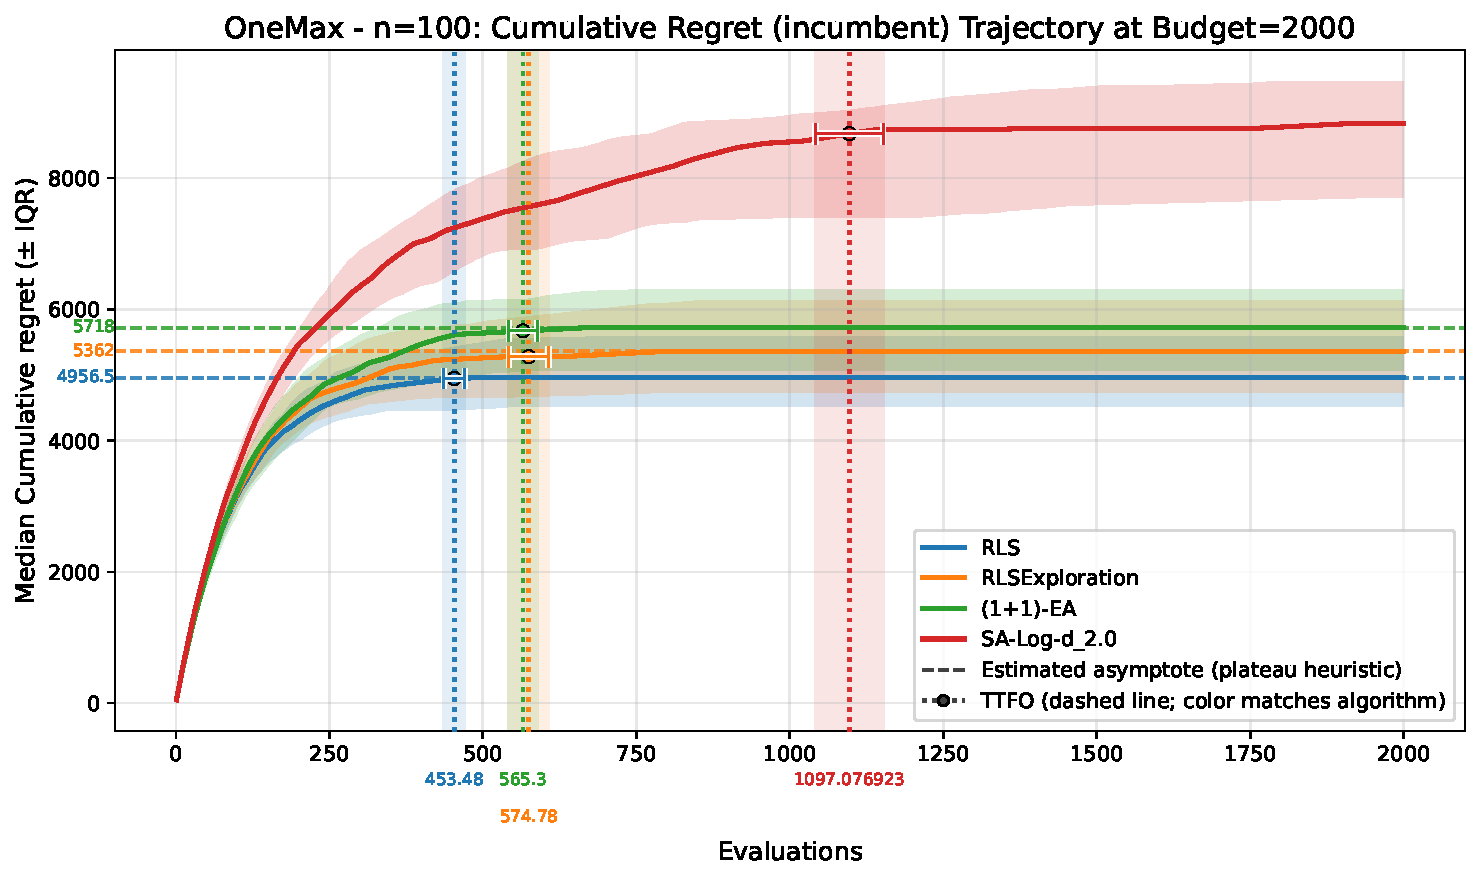
\includegraphics[width=\linewidth]{results/baseline/base/onemax_history_regret_cumulative_best_1.pdf}
    \caption{\textsc{OneMax}.}
    \label{fig:baseline-cr-onemax}
  \end{subfigure}
  \begin{subfigure}[t]{0.48\textwidth}
    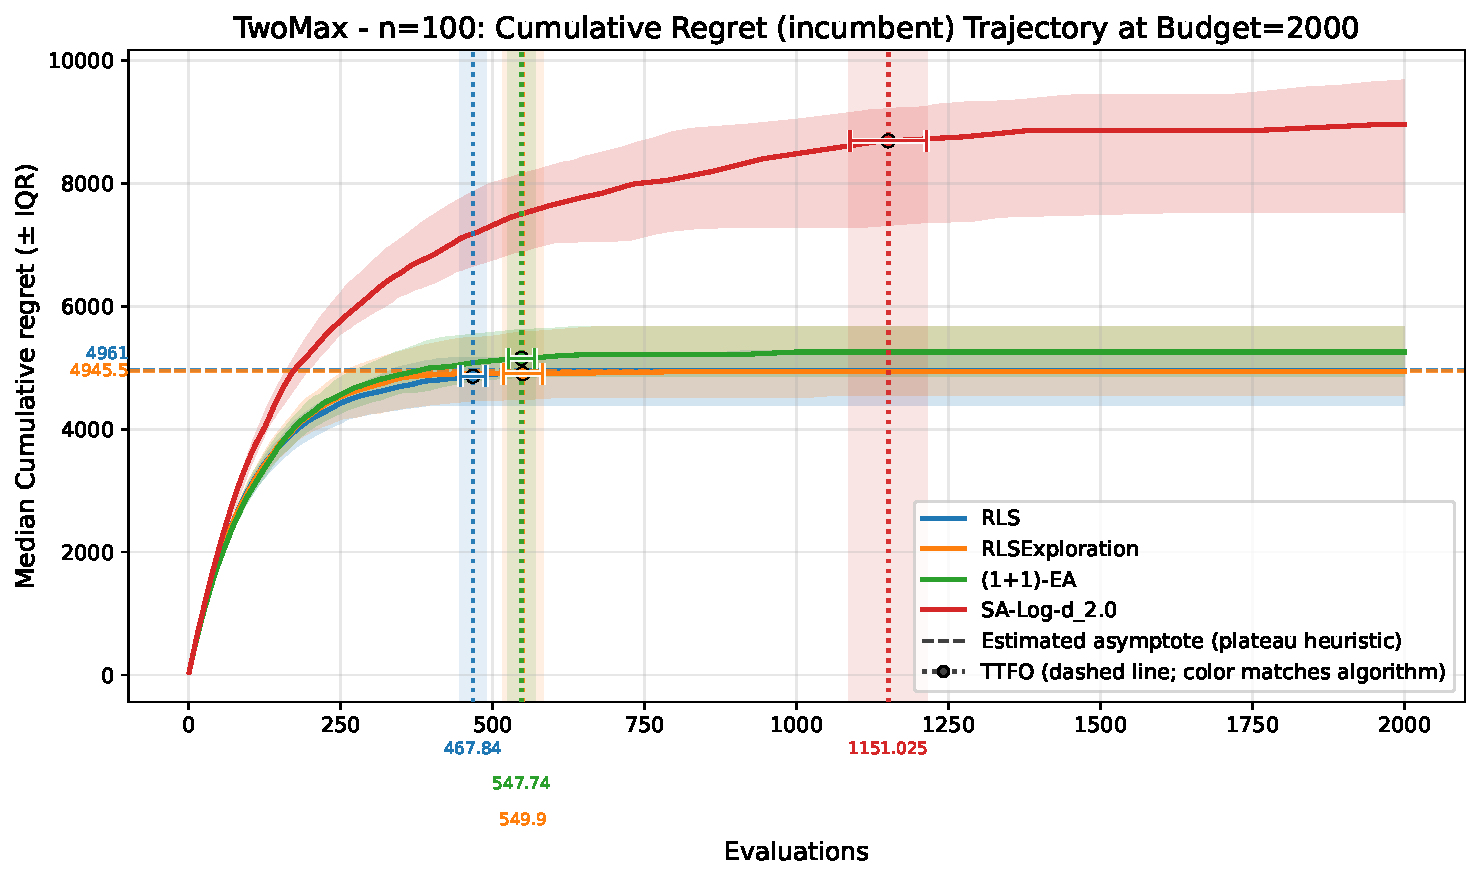
\includegraphics[width=\linewidth]{results/baseline/base/twomax_history_regret_cumulative_best_1.pdf}
    \caption{\textsc{TwoMax}.}
    \label{fig:baseline-cr-twomax}
  \end{subfigure}
  \begin{subfigure}[t]{0.48\textwidth}
    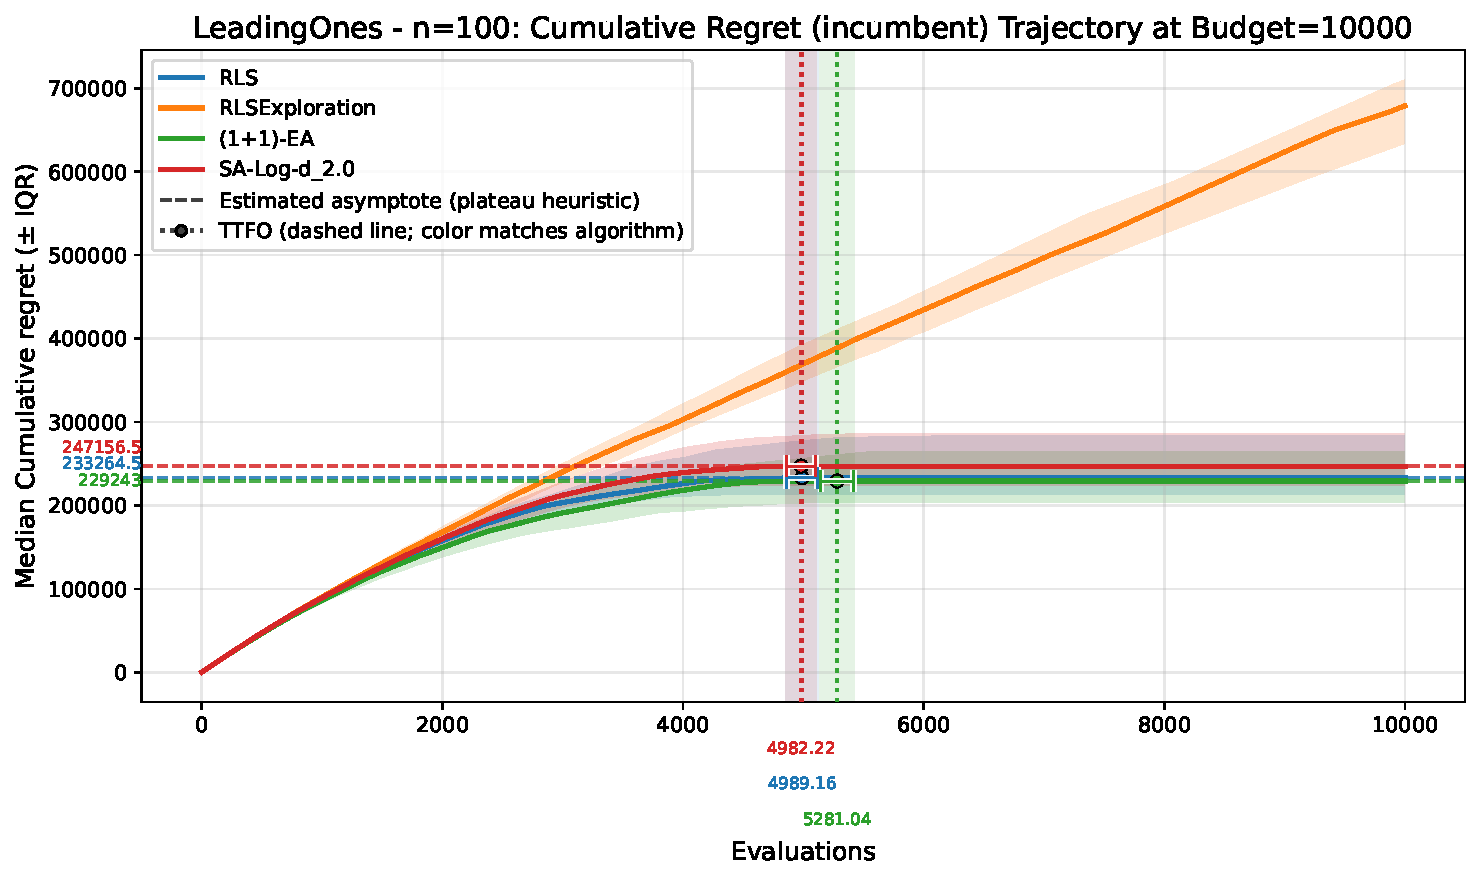
\includegraphics[width=\linewidth]{results/baseline/base/leadingones_history_regret_cumulative_best_1.pdf}
    \caption{\textsc{LeadingOnes}.}
    \label{fig:baseline-cr-leadingones}
  \end{subfigure}
  \begin{subfigure}[t]{0.48\textwidth}
    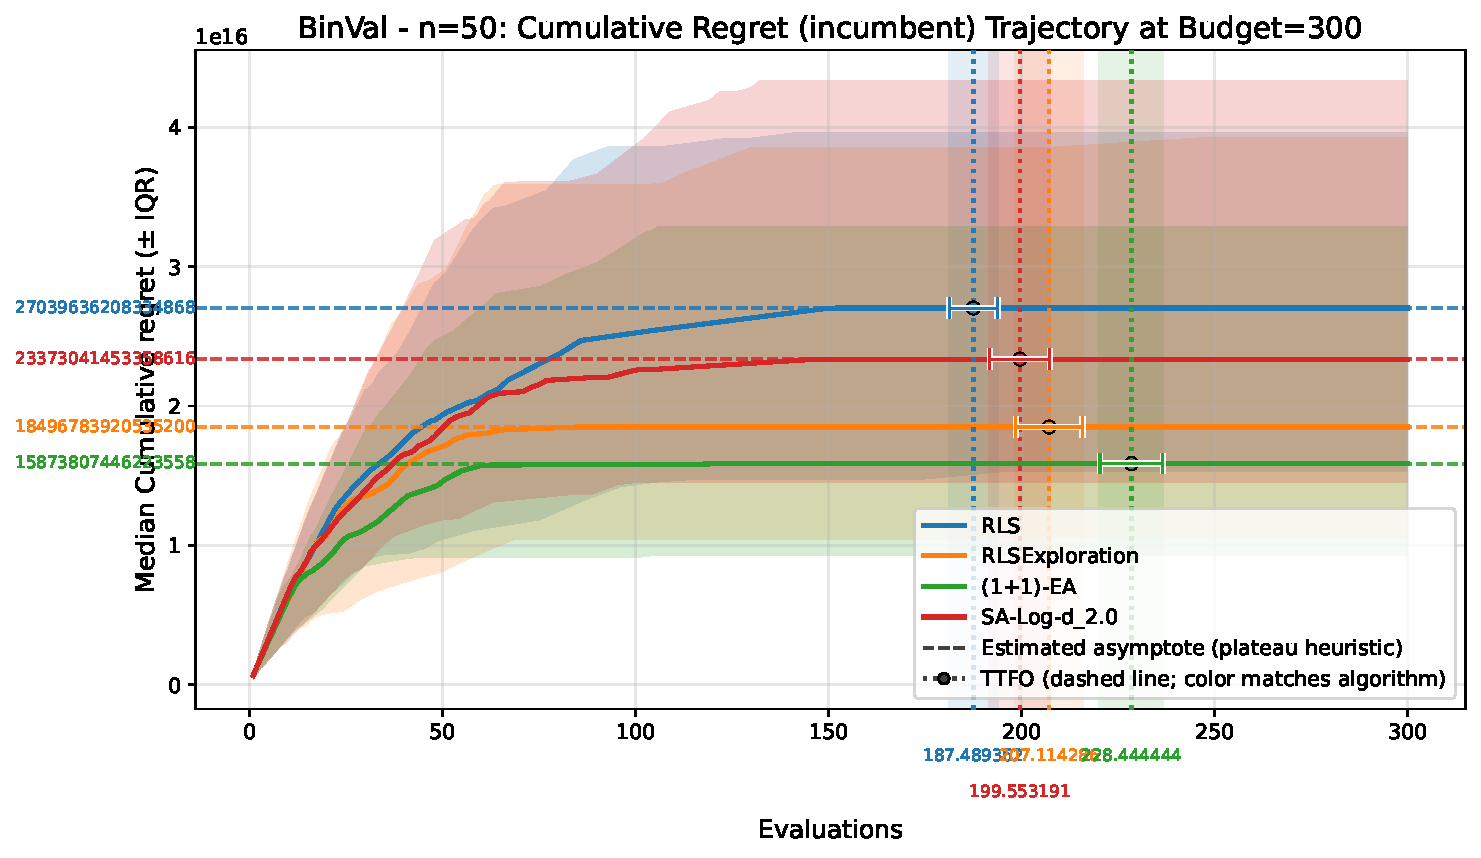
\includegraphics[width=\linewidth]{results/baseline/base/binval_history_regret_cumulative_best_1.pdf}
    \caption{\textsc{BinVal}.}
    \label{fig:baseline-cr-binval}
  \end{subfigure}
  \begin{subfigure}[t]{0.48\textwidth}
    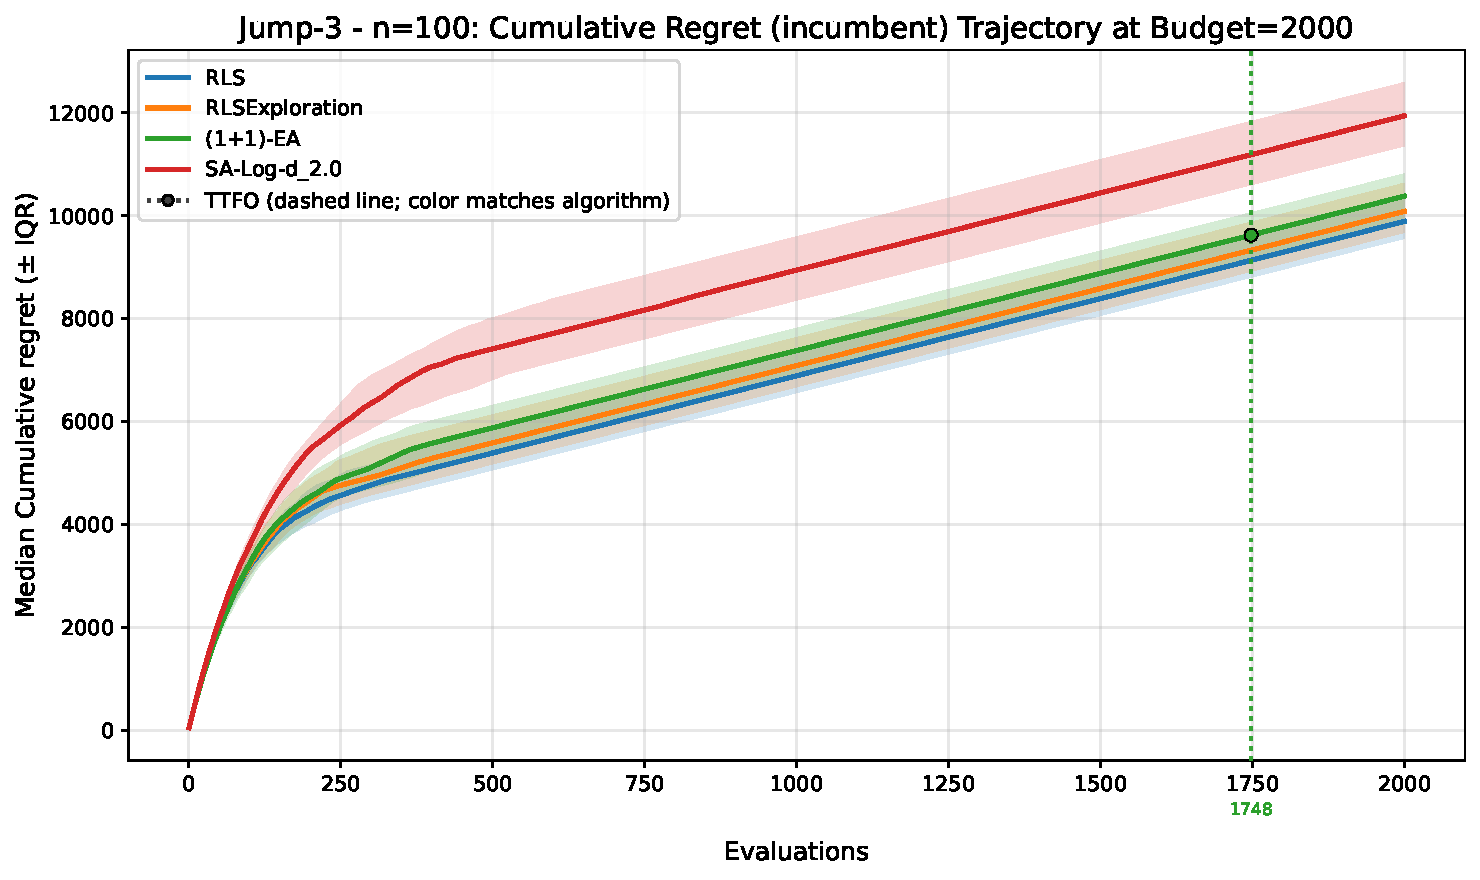
\includegraphics[width=\linewidth]{results/baseline/base/jump-3_history_regret_cumulative_best_1.pdf}
    \caption{\textsc{Jump}-$3$.}
    \label{fig:baseline-cr-jump3}
  \end{subfigure}
  \begin{subfigure}[t]{0.48\textwidth}
    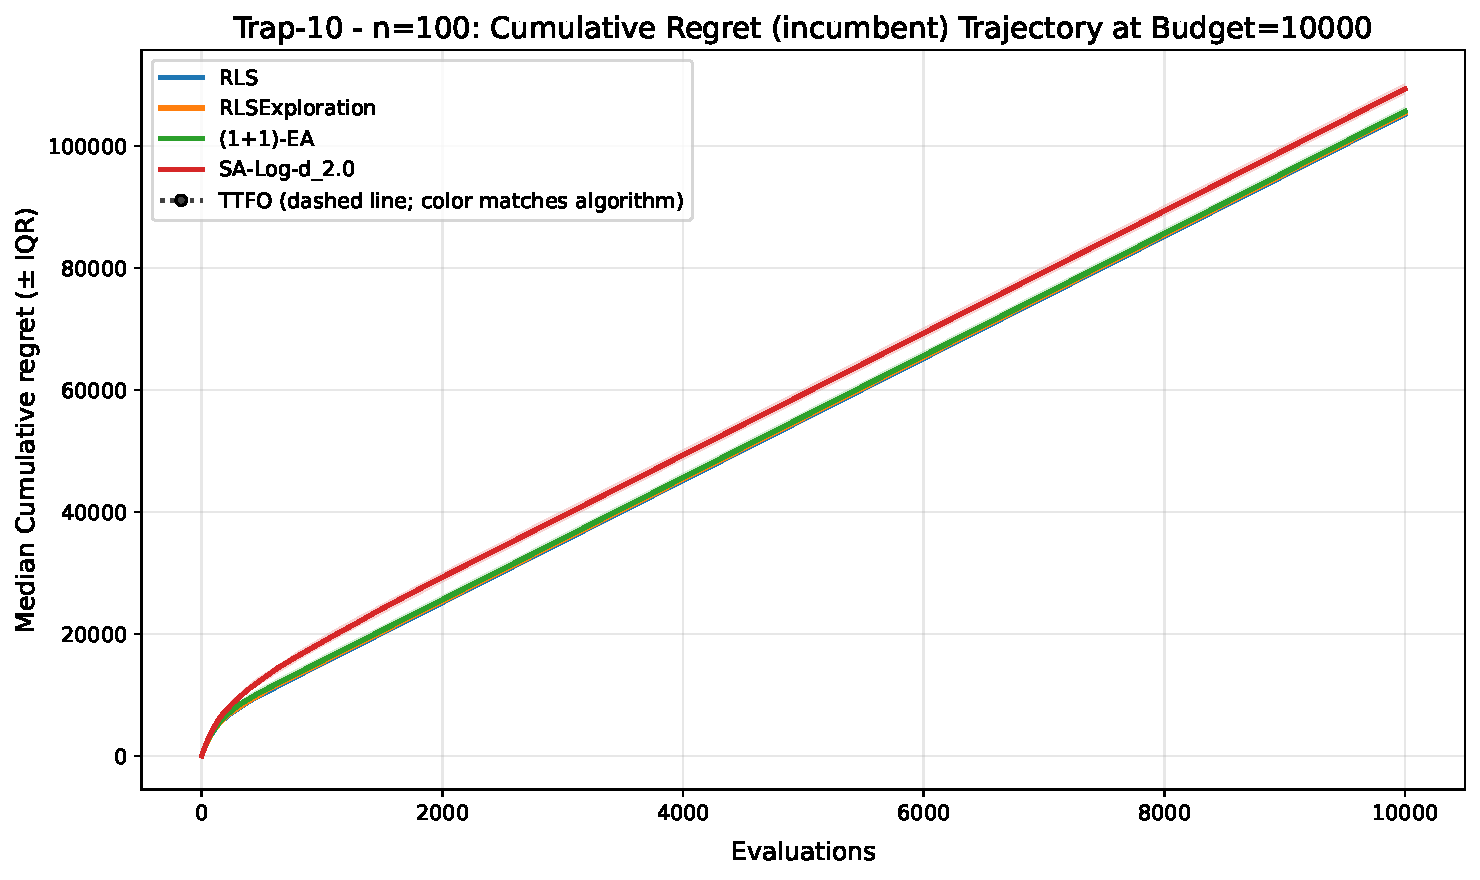
\includegraphics[width=\linewidth]{results/baseline/base/trap-10_history_regret_cumulative_best_1.pdf}
    \caption{\textsc{Trap}-$10$.}
    \label{fig:baseline-cr-trap10}
  \end{subfigure}
  \caption[Suite 01 \acrshort{cr} trajectories]{Suite~01
    incumbent \acrshort{cr} trajectories for the
    baseline pseudo-Boolean problems. Smooth landscapes approach a
    horizontal floor, while barrier and deceptive landscapes retain a
  positive slope under the displayed budget.}
  \label{fig:baseline-cr}
\end{figure}

\subsection{Suite 01: Algorithm-Family Comparison}
\label{sec:results:suite01}
For the simpler \textsc{OneMax} and \textsc{TwoMax} instances, the
relative ordering of mean algorithm performance aligns with the
horizontal convergence points of the median incumbent \acrshort{cr}
curves (Figures~\ref{fig:baseline-cr-onemax}
and~\ref{fig:baseline-cr-twomax}). However, on
\textsc{LeadingOnes} and \textsc{BinVal}, a structural inversion
emerges (Figures~\ref{fig:baseline-cr-leadingones}
and~\ref{fig:baseline-cr-binval}): the algorithms reach the
global optimum in the order \acrshort{rls}, \acrshort{sa}-Log
(d=2.0), \acrshort{rlse}, then $(1+1)$-\acrshort{ea}, yet their
\acrshort{cr} asymptotes are ordered in reverse.

This inversion is consistent with the mechanism described by
Corollary~\ref{cor:asymptotic-regret}:
the asymptote $C = \lim_{T \to \infty} \mathbb{E}[\mathrm{CR}(T)] =
\sum_{v=1}^{f^{*}} \mathbb{E}[\tau_v] - f^{*}$ is governed by
first-hitting times across \emph{all} intermediate fitness
levels. \acrshort{rls}'s greedy trajectory
reaches $f^{*}$ efficiently but lingers at lower fitness levels during
its ascent, inflating the per-level $\mathbb{E}[\tau_v]$ terms and
therefore $C$. The $(1+1)$-\acrshort{ea}'s multi-bit mutation
occasionally promotes the incumbent earlier in the run, reducing those
intermediate contributions and shrinking $C$, despite the later arrival
at $f^{*}$.

For \textsc{Jump} ($k=3$) and \textsc{Trap} ($k=10$), all algorithms
remain trapped in suboptimal basins within the given budget, so
$P(\mathrm{opt}) \approx 0$ and \acrshort{ttfo} is undefined for the
vast majority of runs. The incumbent \acrshort{cr} curves nevertheless
retain diagnostic structure. Each curve grows at an approximately
constant rate, confirming stagnation of the incumbent; the slope at
time $T$ estimates the residual fitness gap $\rho_T^{\mathrm{inc}} =
f^{*} - f(\hat{x}_T)$, so a steeper slope indicates that the
algorithm is trapped further from the optimum and is therefore
incurring a greater per-evaluation cost. The slopes differ across
algorithms, reflecting the fact that each stagnates at a different
local optimum depending on its search strategy, while remaining
non-zero throughout the budget because the landscape barrier (whose
depth is a fixed property of the problem) prevents any
algorithm from closing the gap. This illustrates a key advantage of
\acrshort{cr} over \acrshort{ttfo}: even when convergence is never
observed, the regret trajectory continues to distinguish algorithms
by the quality of their trapped incumbent, information that a binary
optimum achievement measure cannot provide.



\subsection{Suite 02: Extended Pseudo-Boolean Benchmark}
\label{sec:results:suite02}
%
Suite~02 shows that the Suite~01 ordering generalizes only on the smooth
part of the benchmark.

\begin{figure}[!htbp]
  \centering
  \begin{subfigure}[t]{0.48\textwidth}
    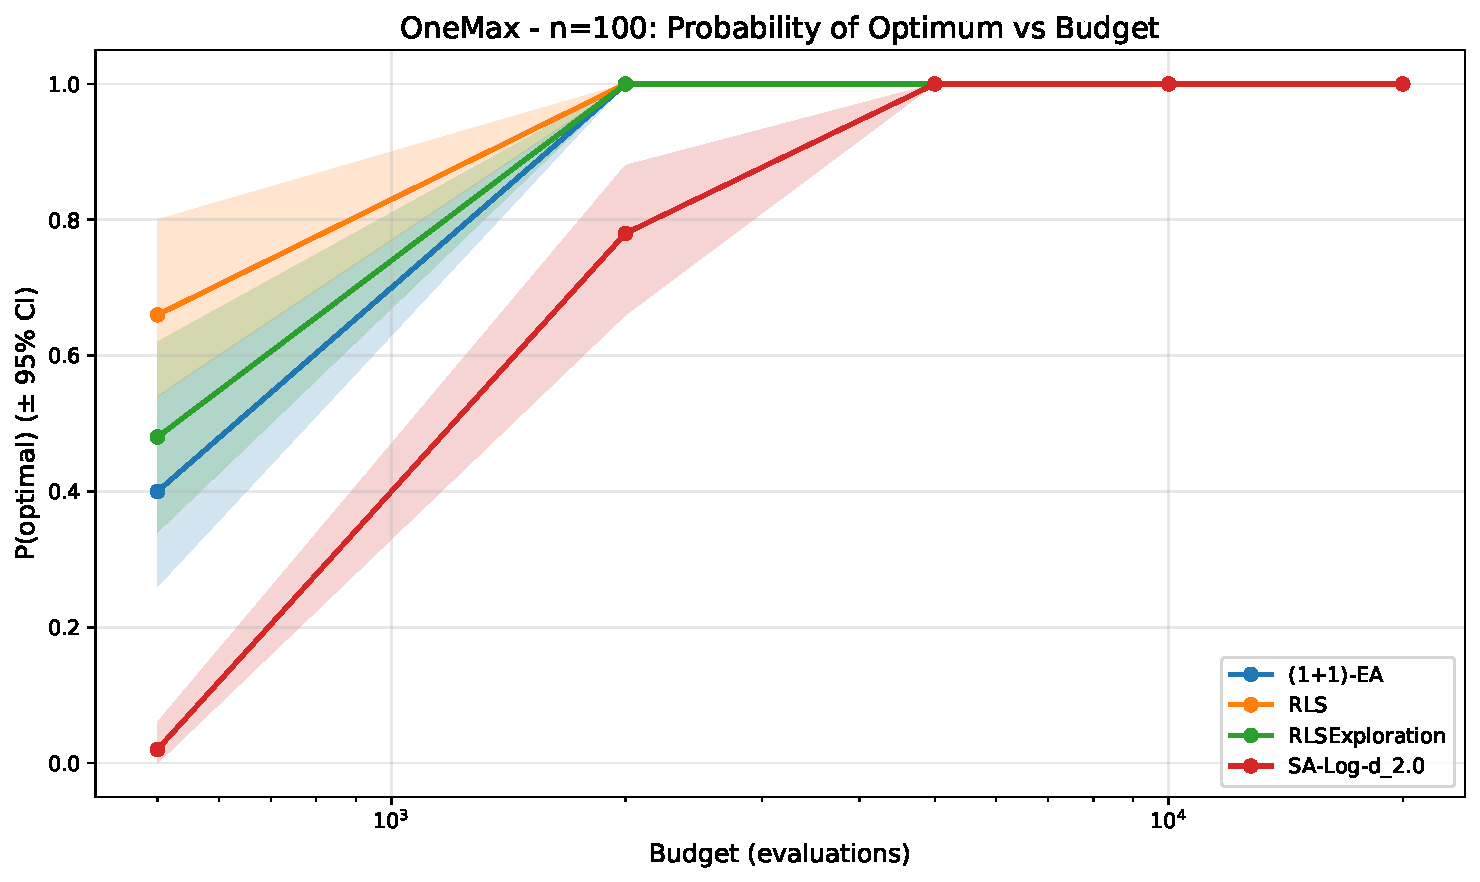
\includegraphics[width=\linewidth]{results/baseline/ext/onemax_convergence_probability.pdf}
    \caption{\textsc{OneMax} convergence probability.}
    \label{fig:suite02-onemax-cdp}
  \end{subfigure}
  \begin{subfigure}[t]{0.48\textwidth}
    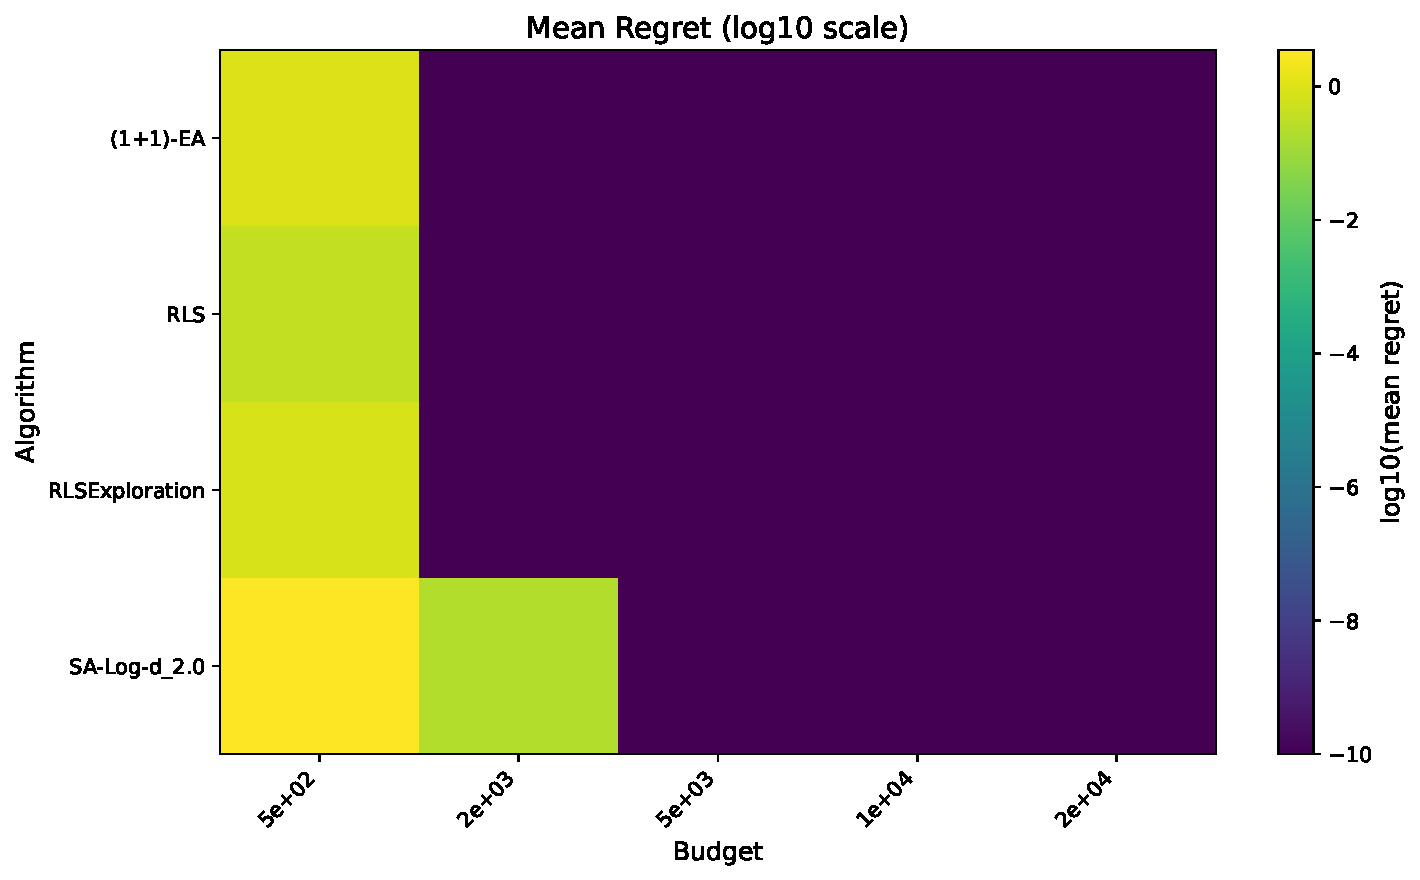
\includegraphics[width=\linewidth]{results/baseline/ext/onemax_comparison_heatmap.pdf}
    \caption{\textsc{OneMax} mean-regret heat map.}
    \label{fig:suite02-onemax-heatmap}
  \end{subfigure}
  \begin{subfigure}[t]{0.48\textwidth}
    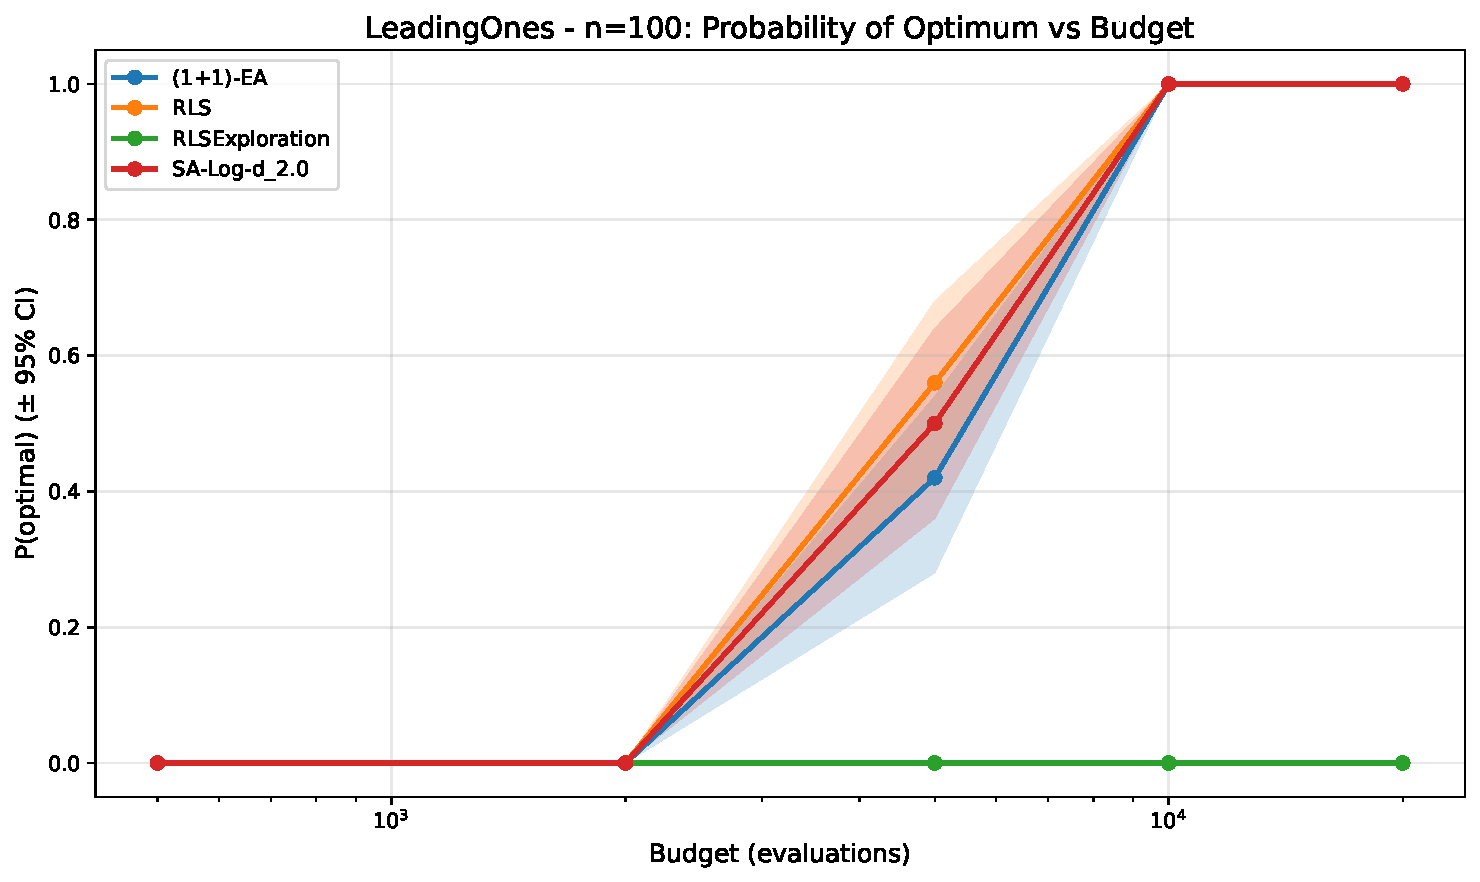
\includegraphics[width=\linewidth]{results/baseline/ext/leadingones_convergence_probability.pdf}
    \caption{\textsc{LeadingOnes} convergence probability.}
    \label{fig:suite02-leadingones-cdp}
  \end{subfigure}
  \begin{subfigure}[t]{0.48\textwidth}
    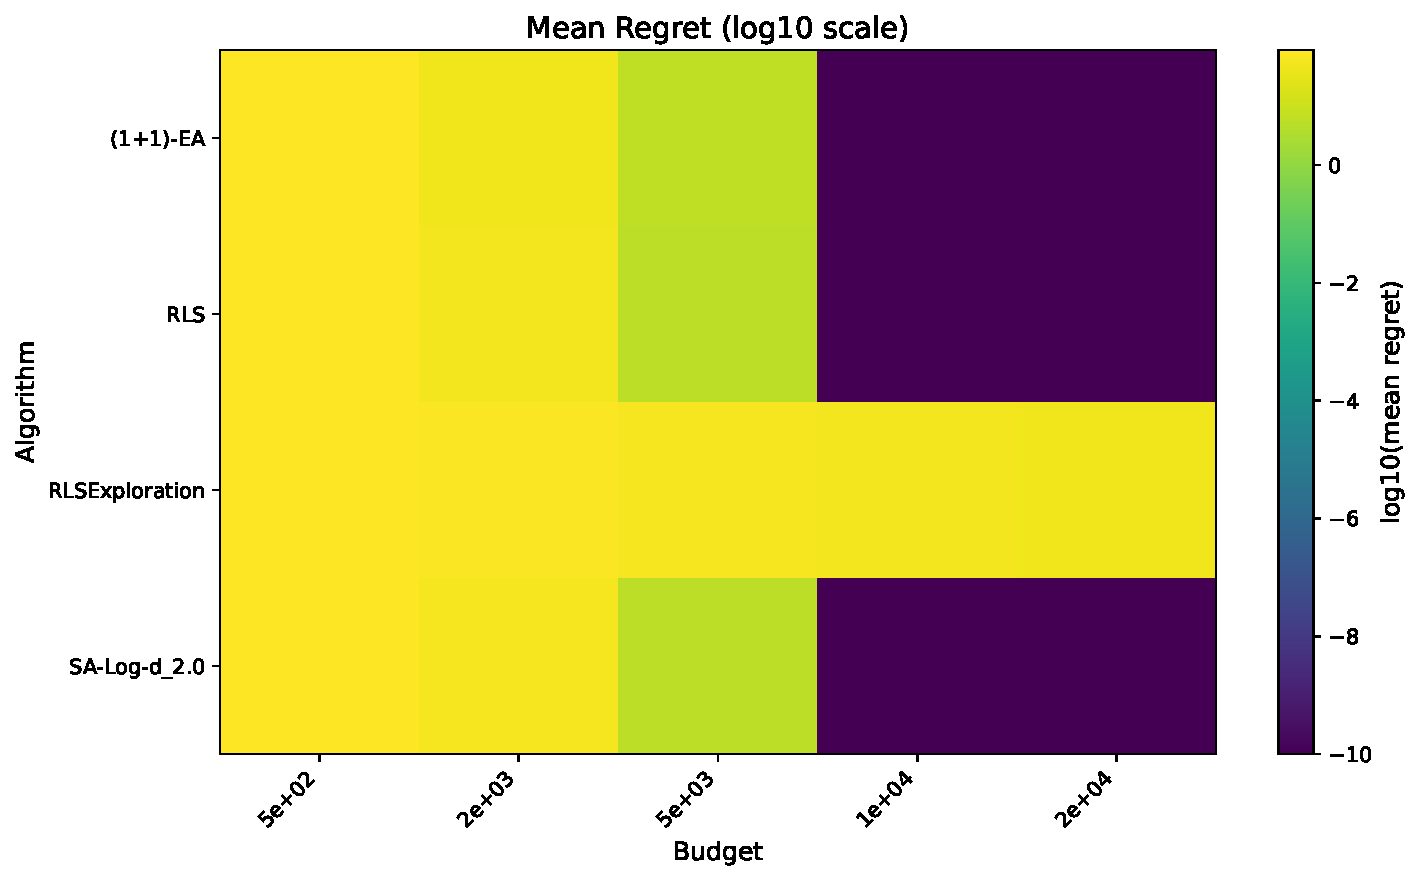
\includegraphics[width=\linewidth]{results/baseline/ext/leadingones_comparison_heatmap.pdf}
    \caption{\textsc{LeadingOnes} mean-regret heat map.}
    \label{fig:suite02-leadingones-heatmap}
  \end{subfigure}
  \begin{subfigure}[t]{0.48\textwidth}
    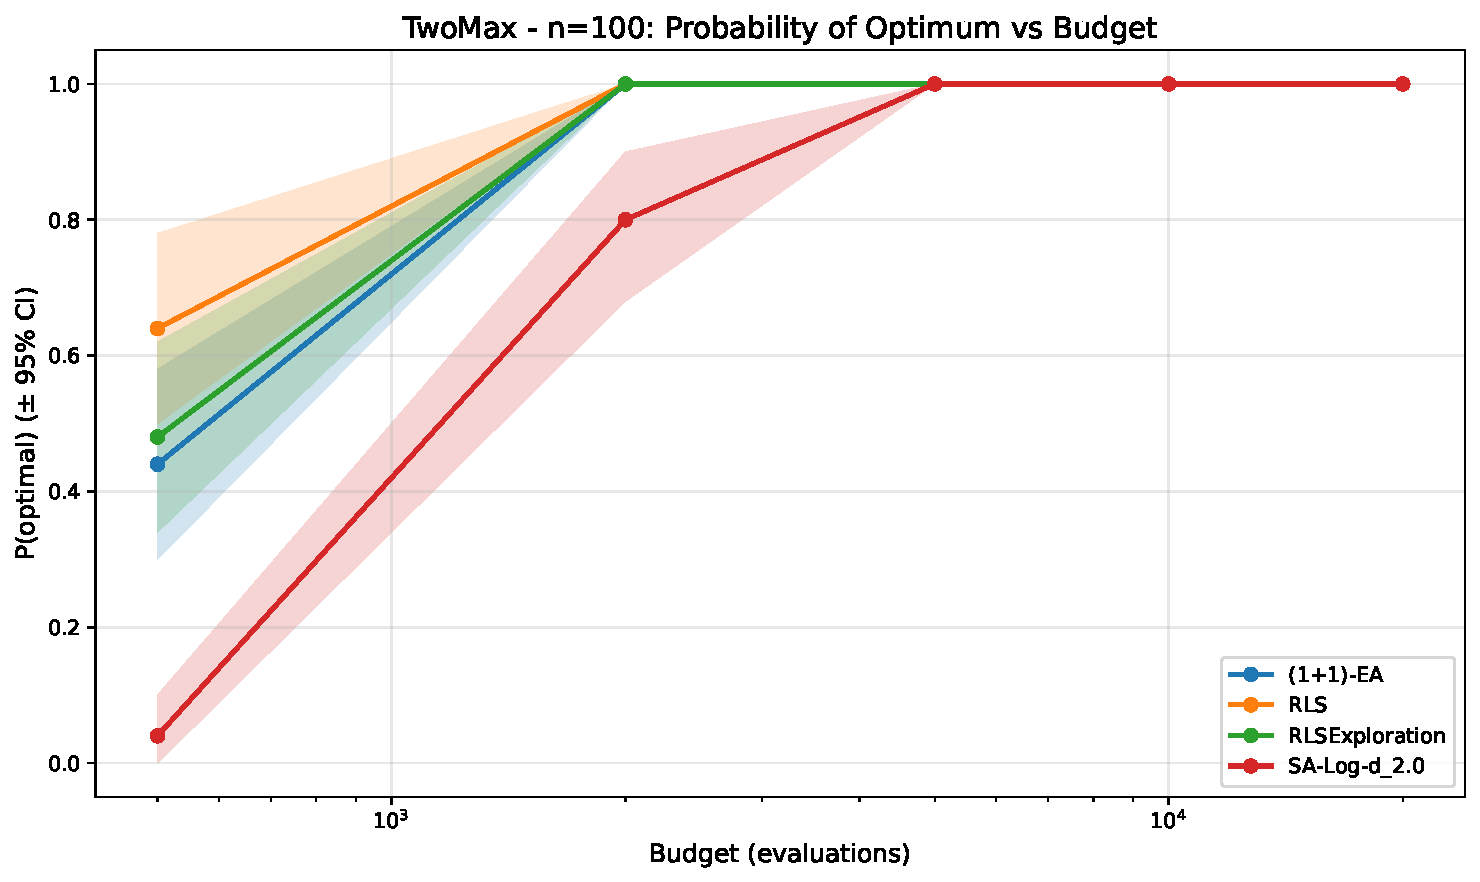
\includegraphics[width=\linewidth]{results/baseline/ext/twomax_convergence_probability.pdf}
    \caption{\textsc{TwoMax} convergence probability.}
    \label{fig:suite02-twomax-cdp}
  \end{subfigure}
  \begin{subfigure}[t]{0.48\textwidth}
    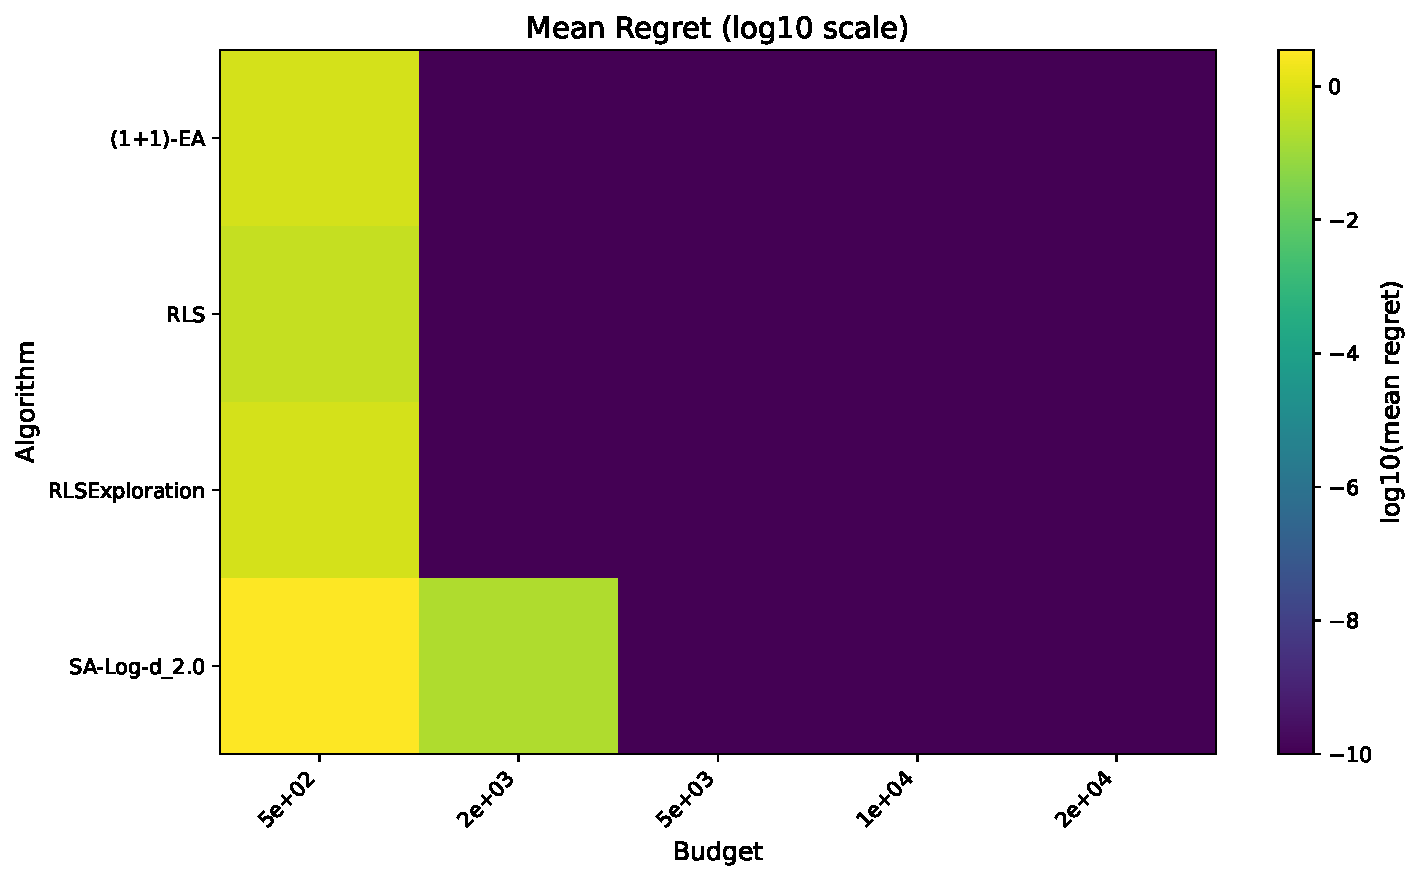
\includegraphics[width=\linewidth]{results/baseline/ext/twomax_comparison_heatmap.pdf}
    \caption{\textsc{TwoMax} mean-regret heat map.}
    \label{fig:suite02-twomax-heatmap}
  \end{subfigure}
  \caption[Suite 02 easy-tier summary plots]{Suite~02 easy-tier
    summary plots. Convergence probabilities and
    mean-regret heat maps show that the baseline algorithm ordering is stable
  on smooth benchmark problems under the extended budget.}
  \label{fig:suite02-easy-summary}
\end{figure}

\begin{figure}[!htbp]
  \centering
  \begin{subfigure}[t]{0.48\textwidth}
    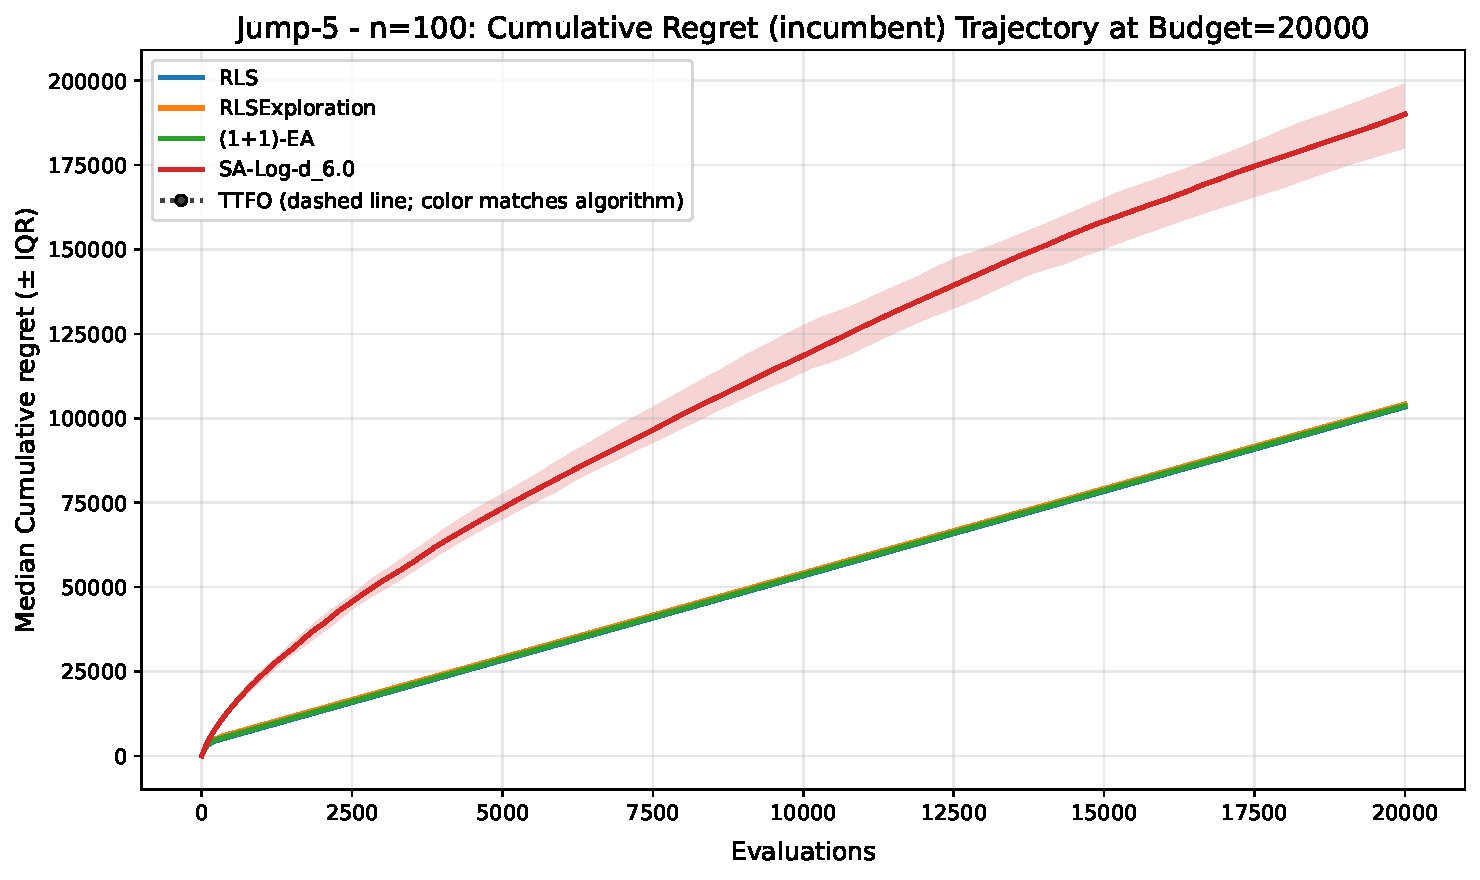
\includegraphics[width=\linewidth]{results/baseline/ext/jump-5_history_regret_cumulative_best.pdf}
    \caption{\textsc{Jump}-$5$ cumulative regret.}
    \label{fig:suite02-jump5-cr}
  \end{subfigure}
  \begin{subfigure}[t]{0.48\textwidth}
    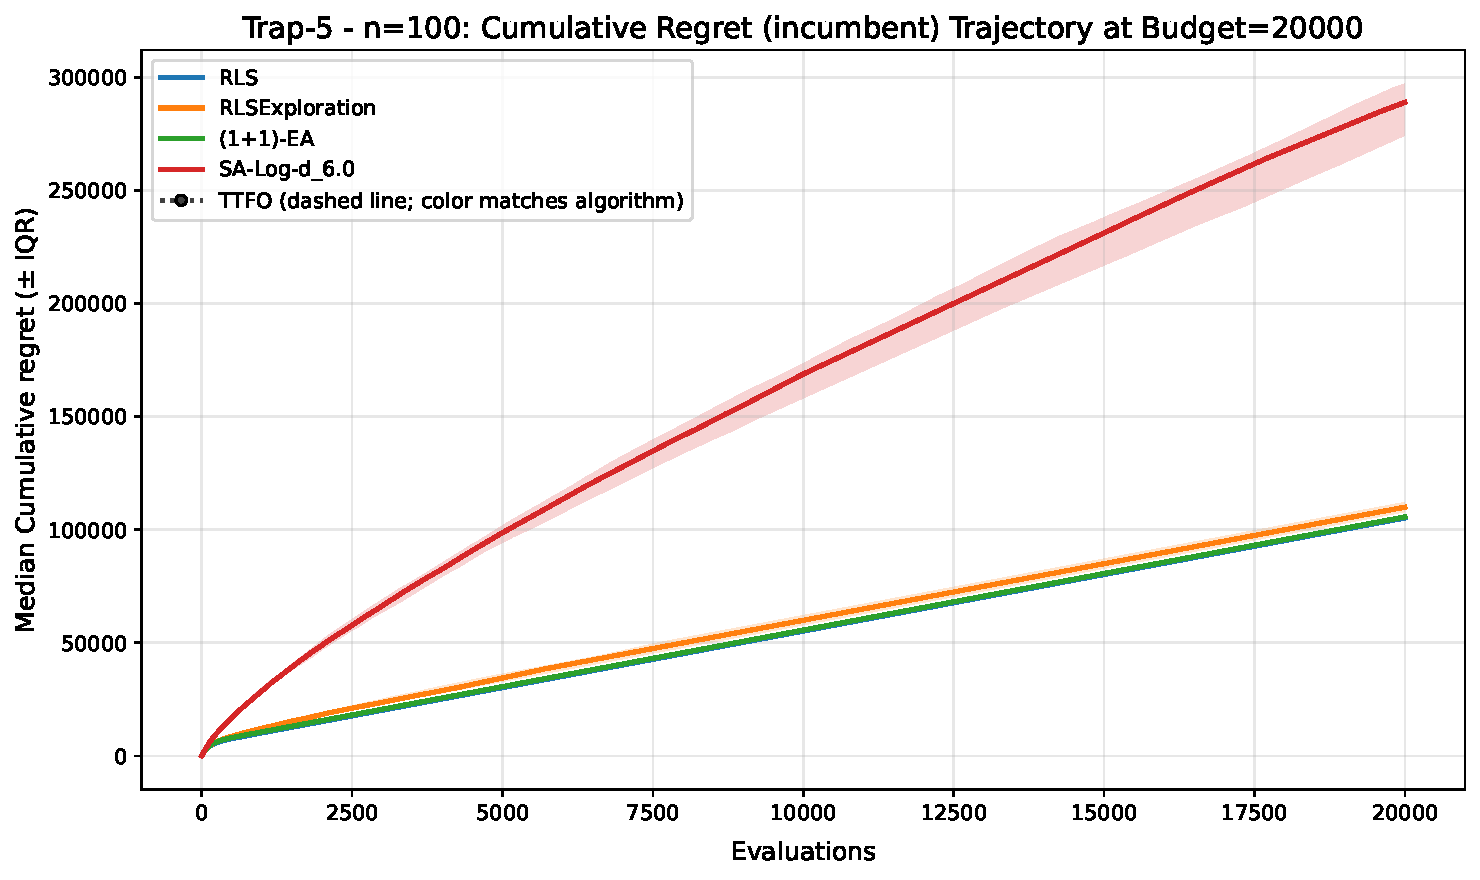
\includegraphics[width=\linewidth]{results/baseline/ext/trap-5_history_regret_cumulative_best.pdf}
    \caption{\textsc{Trap}-$5$ cumulative regret.}
    \label{fig:suite02-trap5-cr}
  \end{subfigure}
  \begin{subfigure}[t]{0.80\textwidth}
    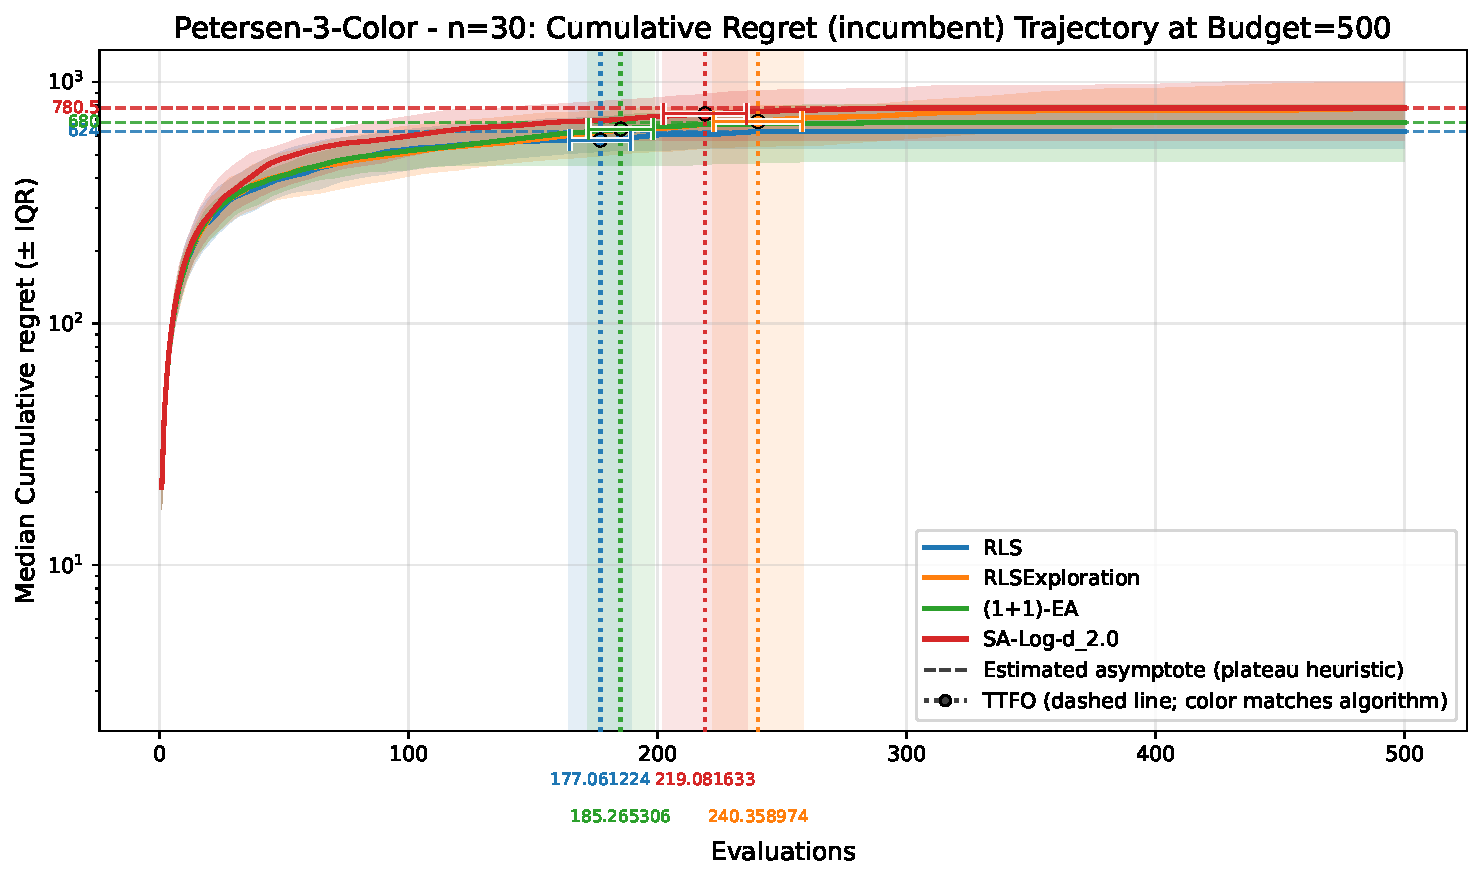
\includegraphics[width=\linewidth]{results/baseline/ext/petersen-3-color_history_regret_cumulative_best.pdf}
    \caption{\textsc{Petersen}-3-colour cumulative regret.}
    \label{fig:suite02-petersen-cr}
  \end{subfigure}
  \caption[Suite 02 harder-instance regret trajectories]{Selected
    Suite~02 \acrshort{cr} trajectories for harder
    benchmark instances. The barrier problems retain sustained regret growth,
  while the graph-colouring instance is solved within the displayed budget.}
  \label{fig:suite02-selected-cr}
\end{figure}

On \textsc{OneMax}, \textsc{LeadingOnes}, and
\textsc{TwoMax}, the same separation between the four algorithm families is
visible in both convergence probability and the mean-regret heat map
Figures~\ref{fig:suite02-easy-summary}, so the
baseline ranking is stable under the extended budget.

The barrier problems change the picture.
Persistent \acrshort{rlse} exploration with $\varepsilon=0.05$
improves barrier escape.
On \textsc{Jump-3}, this changes the post-stagnation ordering of the
incumbent \acrshort{cr} curves: with fixed $\varepsilon=0.05$,
\acrshort{rlse} receives more frequent opportunities to leave the local
basin than under the Suite~01 default $\varepsilon=0.01$.

The ``hotter'' SA schedule ($d=6.0$) on \textsc{Jump-5} and \textsc{Trap-5}
reduces premature freezing, as seen by higher \acrshort{iqr} in
Figures~\ref{fig:suite02-jump5-cr} and~\ref{fig:suite02-trap5-cr}.

On \acrshort{hiff}-64 no method reaches the optimum within budget, so this
instance is retained as a hard hierarchical case rather than a convergence
benchmark.

In contrast, \textsc{Petersen-3-Color} is solved by all four
algorithms within budget, with convergence concentrated around
200--300 evaluations (Figure~\ref{fig:suite02-petersen-cr}).

\section{Verification Suite}
\label{sec:results:verification}
The verification compares two curves indexed by evaluation time: the
empirical mean cumulative regret $\bar R_t$ and the profile-derived
quantity $\hat R_t$. Since Theorem~\ref{thm:regret-profile} asserts an
identity over the full trajectory, not just at the final horizon, the
comparison is performed pointwise over $t=1,\ldots,T$.

Three complementary error summaries are reported
(Table~\ref{tab:vermeas}). The \acrfull{rmse} measures the
typical global discrepancy between the two curves and is sensitive to
persistent deviations across the horizon. The
\acrfull{mae}~\cite{higham2002acc} records the worst pointwise
discrepancy and therefore checks
whether the identity fails locally at any evaluation index. Finally, the
\acrfull{rmae} normalizes this worst-case gap
by the scale of the empirical cumulative regret curve, allowing results
to be compared across problems with very different regret magnitudes.
Together, these measures test both average agreement and worst-case
pointwise agreement.

\begin{table}[!htbp]
  \centering
  \begin{tabular}{lll}
    \toprule
    Measure & Formula & Interpretation \\
    \midrule
    \acrshort{rmse}
    & $\sqrt{\dfrac{1}{T}\sum_{t=1}^{T}\left(\hat{R}_t-\bar{R}_t\right)^2}$
    & Average curve-level discrepancy \\[1.4em]

    \acrshort{mae}
    & $\max_t \left|\hat{R}_t-\bar{R}_t\right|$
    & Worst pointwise discrepancy \\[0.8em]

    \acrshort{rmae}
    & $\dfrac{\max_t \left|\hat{R}_t-\bar{R}_t\right|}{\max_t \bar{R}_t}$
    & Scale-normalized worst-case discrepancy \\
    \bottomrule
  \end{tabular}
  \caption[Profile verification error measures]{Error measures used
    to compare profile-derived ($\hat{R}_t$) and
    empirical ($\bar{R}_t$) expected cumulative regret
    $\mathbb{E}[\mathrm{CR}(T)]$
  at each evaluation index $t$.}
  \label{tab:vermeas}
\end{table}

The verification is accepted if the profile-derived and empirical curves
satisfy two conditions: first, the relative maximum pointwise error must
remain below $1\%$,
\[
  \frac{\max_t |\hat R_t-\bar R_t|}{\max_t \bar R_t} < 0.01,
\]
and second, the normalized RMSE,
\[
  \frac{\mathrm{RMSE}}{\max_t \bar R_t},
\]
must be of the same order or smaller. These thresholds are deliberately
scale-normalized, so that the criterion is not biased against problems
such as \textsc{LeadingOnes}, where cumulative regret is naturally much
larger in absolute value.

\subsection{Suite 08: Runtime Profile Verification}
\label{sec:results:suite08}

\begin{figure}[!htbp]
  \centering
  \begin{subfigure}[t]{0.80\textwidth}
    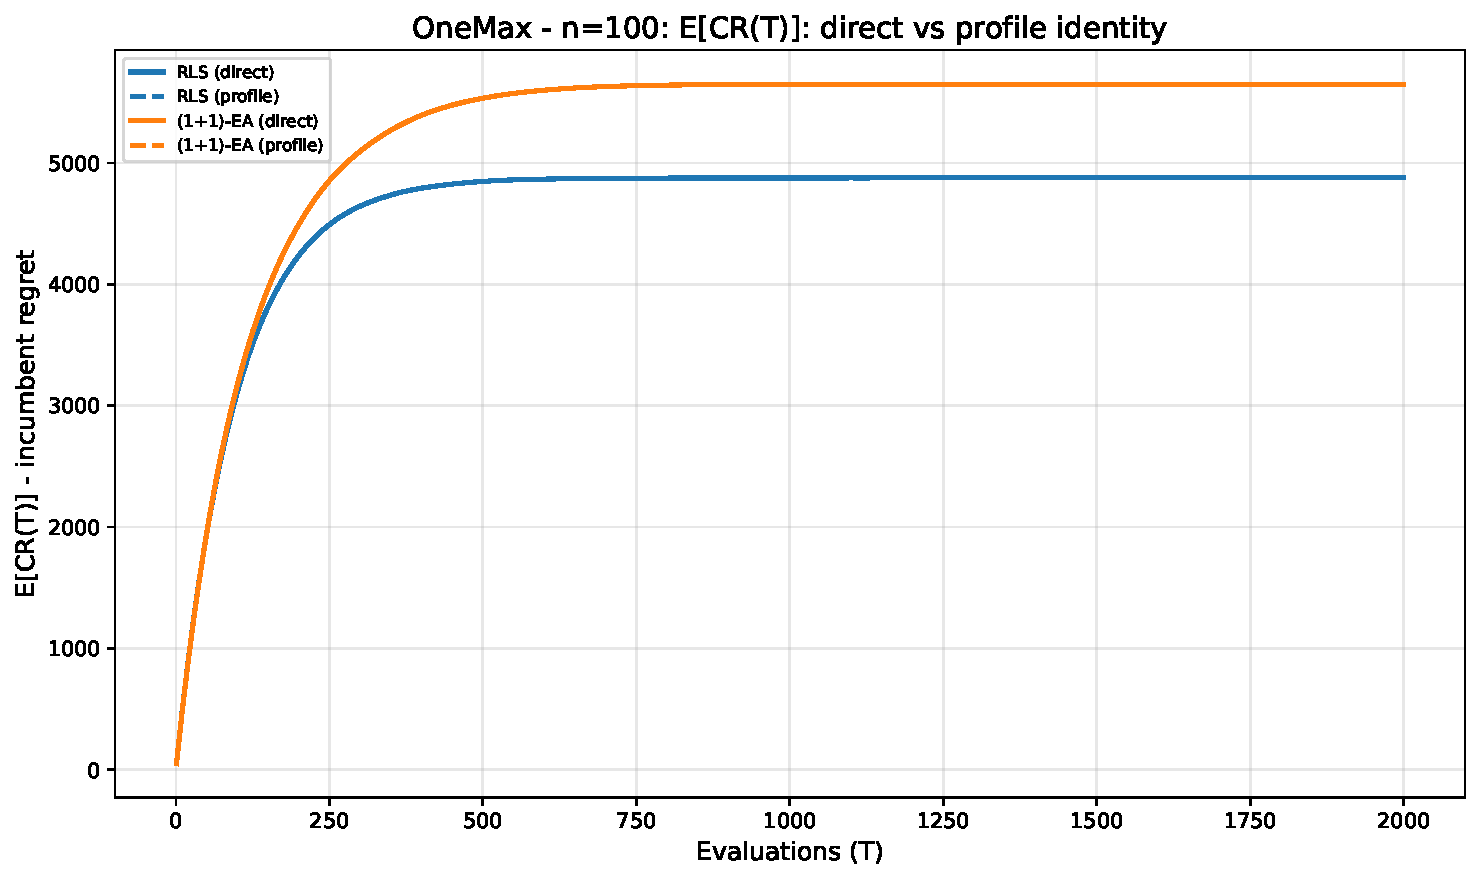
\includegraphics[width=\linewidth]{results/verification/cr_prof_ver_onemax.pdf}
    \caption[\textsc{OneMax} verification plots]{Verification plots
      for \acrshort{rls} (black) and
      $(1+1)$-\acrshort{ea} (blue) for the \textsc{OneMax} problem,
    with maximum budget 2\,000}
  \end{subfigure}
  \begin{subfigure}[t]{0.80\textwidth}
    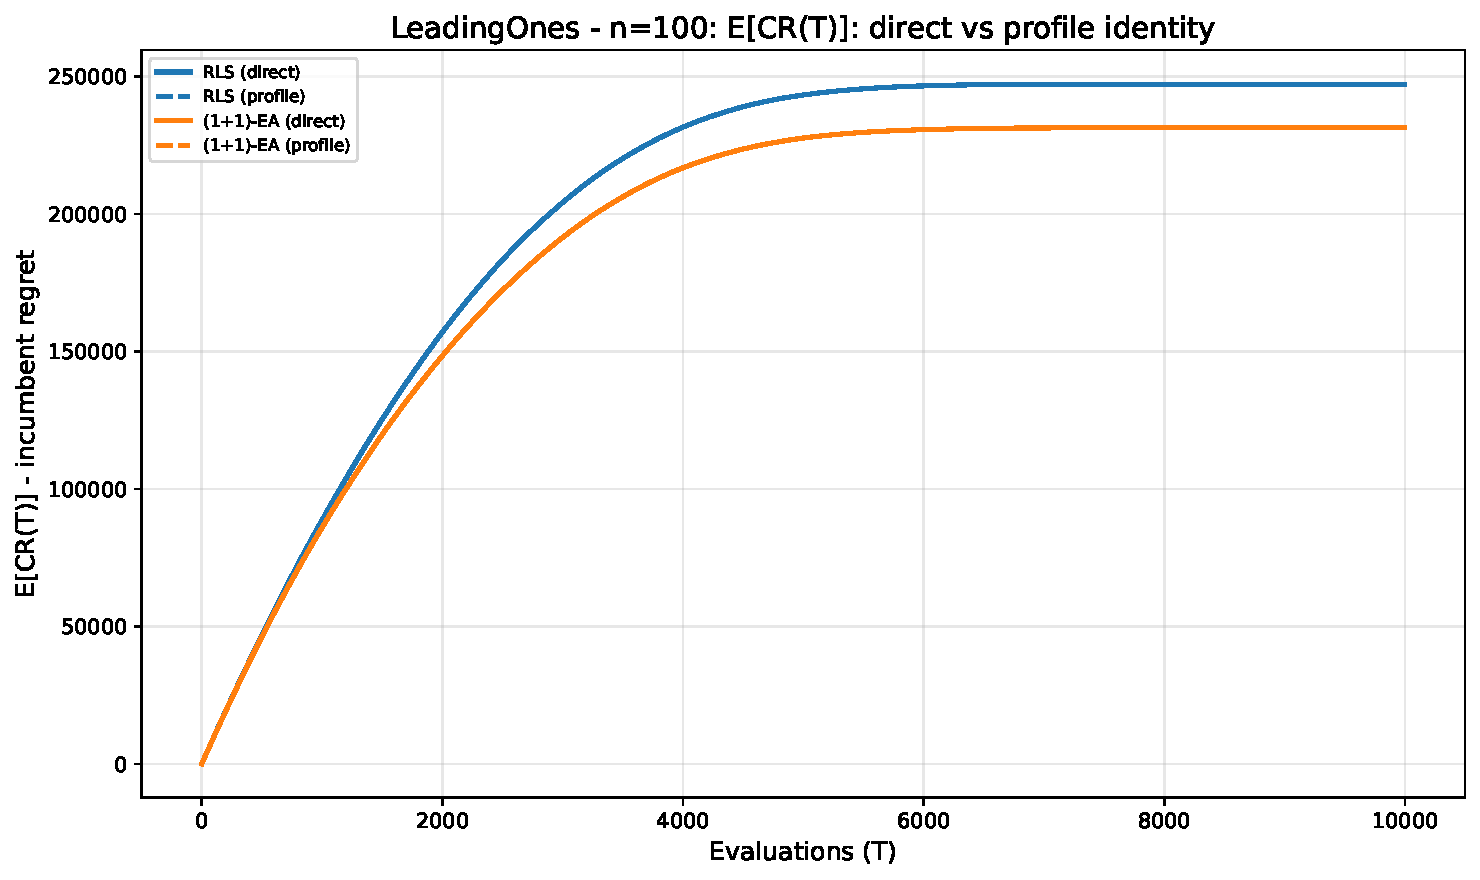
\includegraphics[width=\linewidth]{results/verification/cr_prof_ver_leadingones.pdf}
    \caption[\textsc{LeadingOnes} verification plots]{Verification
      plots for \acrshort{rls} (black) and
      $(1+1)$-\acrshort{ea} (blue) for the \textsc{LeadingOnes}
    problem, with maximum budget 10\,000}
  \end{subfigure}
  \caption[Empirical and profile-derived verification curves]{The
    verification curves for the empirically calculated
    mean \acrshort{cr} ($\mathbb{E}[\mathrm{CR}(T)]$, solid plot) and
  the profile-derived expected \acrshort{cr} ($\hat{R}_t$, dotted plot)}
\end{figure}

\begin{table}[!htbp]
  \centering
  \small
  \begin{tabular}{llccc}
    \toprule
    Problem & Algorithm & \acrshort{rmse} & \acrshort{mae} & \acrshort{rmae} \\
    \midrule
    \multirow{2}{8.5em}{\textsc{OneMax} (Budget: 2\,000)}
      & $(1+1)$-\acrshort{ea} & $8.90\times10^{-12}$ & $1.18\times10^{-11}$ & $2.09\times10^{-15}$ \\
      & \acrshort{rls}        & $3.02\times10^{-12}$ & $4.55\times10^{-12}$ & $9.33\times10^{-16}$ \\
    \midrule
    \multirow{2}{8.5em}{\textsc{LeadingOnes} (Budget: 10\,000)}
      & $(1+1)$-\acrshort{ea} & $1.37\times10^{-9}$ & $2.82\times10^{-9}$ & $1.22\times10^{-14}$ \\
      & \acrshort{rls}        & $3.57\times10^{-9}$ & $5.76\times10^{-9}$ & $2.33\times10^{-14}$ \\
    \bottomrule
  \end{tabular}
  \caption[Pointwise profile verification distances]{Pointwise
    distances between the empirically calculated $\mathbb{E}[\mathrm{CR}]$
    and the distributional profile-derived $\mathrm{CR}$.}
  \label{tab:profile-verification-distances}
\end{table}
\FloatBarrier

The profile identity holds to floating-point precision across all four
combinations. The largest \acrshort{mae} is $5.76\times10^{-9}$, and the
largest \acrshort{rmae} is only $2.33\times10^{-14}$.
Thus, on integer-valued benchmarks with exact fitness levels and complete time
grids, the direct trajectory average and the profile-derived tail-sum curve are
numerically indistinguishable (Table~\ref{tab:profile-verification-distances}).

This agreement is stronger than what would be expected from an independent
Monte-Carlo comparison because the two curves are computed from the same
$R=100$ runs. Sampling variation affects which trajectories are observed, but
both curves are deterministic transformations of that same sample. The
pointwise comparison therefore tests implementation agreement: for OneMax and
LeadingOnes, the profile calculation uses the exact integer fitness levels
$1,\ldots,100$ and every evaluation time point at the displayed budgets. The
remaining differences are therefore numerical round-off. 
The separate discretization caveat applies later to
real-valued landscapes such as NK.
\begin{figure}[!htbp]
  \centering
  \begin{subfigure}[t]{0.49\textwidth}
    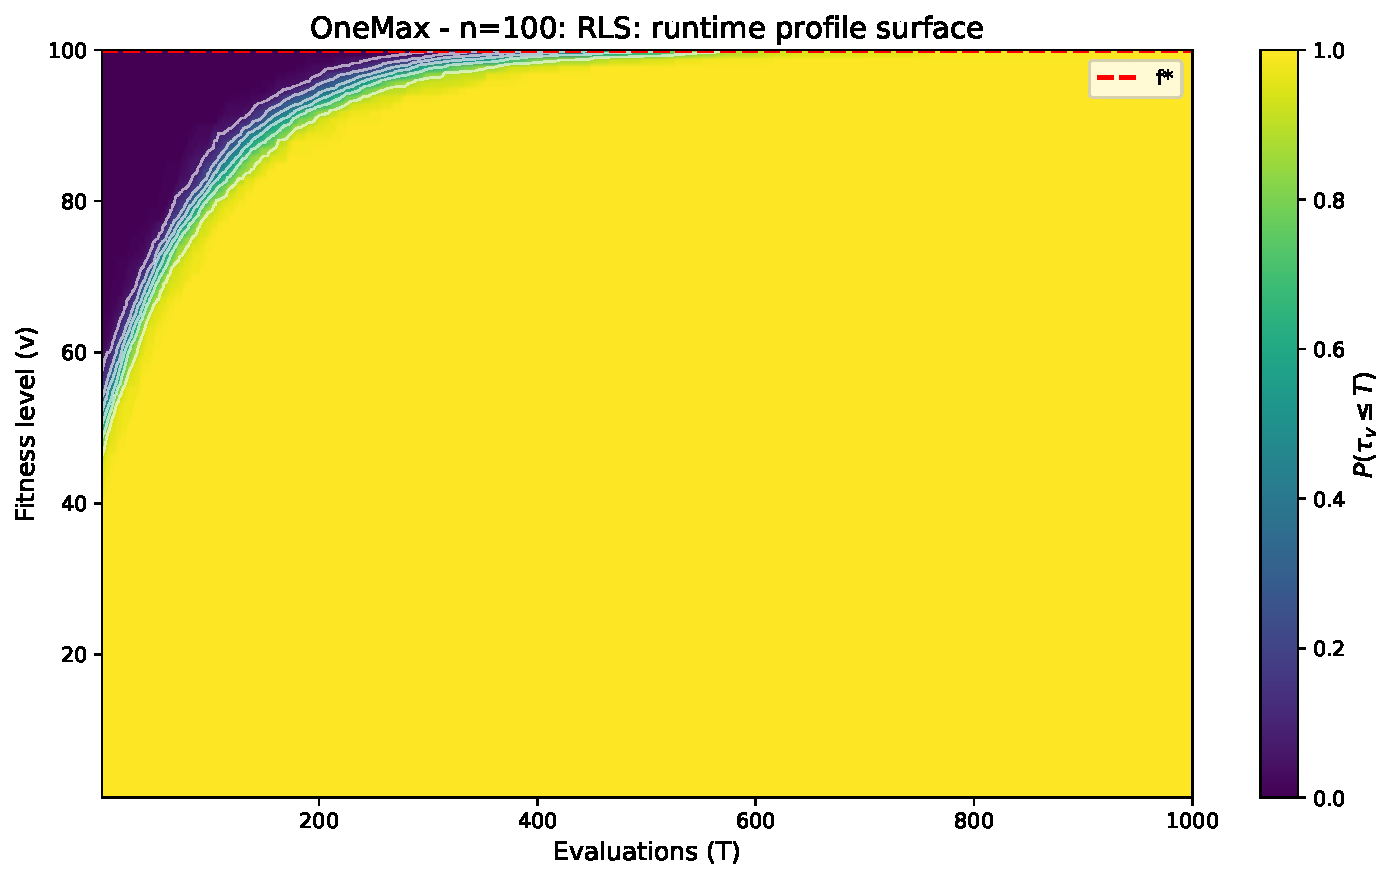
\includegraphics[width=\linewidth]{results/verification/inv_prof_surf_onemax_RLS.pdf}
    \caption[\acrshort{rls} profile on
    \textsc{OneMax}]{\acrshort{rls} for the \textsc{OneMax} problem, with
    displayed profile horizon 1\,000}
  \end{subfigure}
  \begin{subfigure}[t]{0.49\textwidth}
    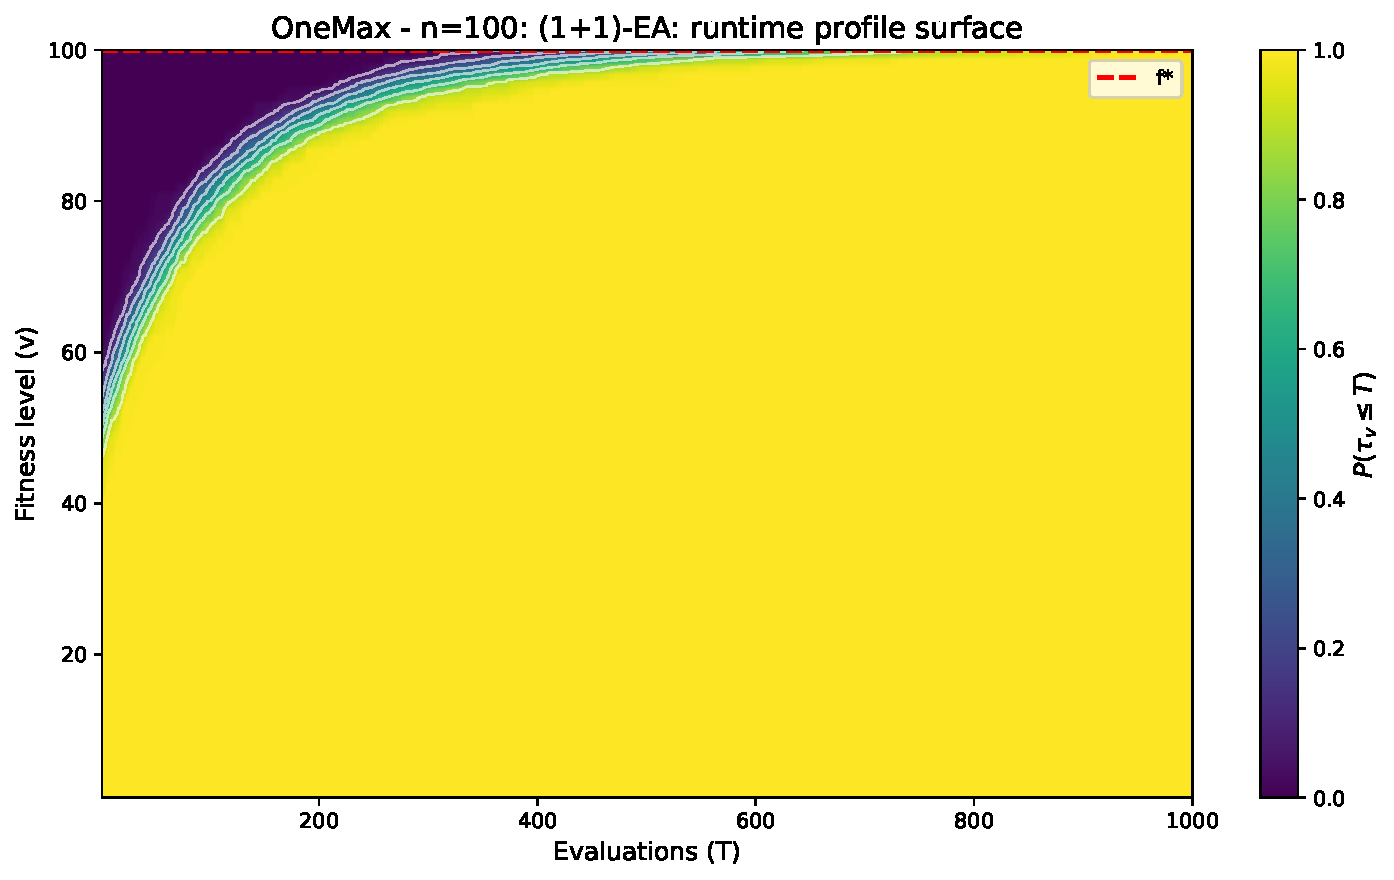
\includegraphics[width=\linewidth]{results/verification/inv_prof_surf_onemax_(1+1)-EA.pdf}
    \caption[$(1+1)$-\acrshort{ea} profile on
    \textsc{OneMax}]{$(1+1)$-\acrshort{ea} for the \textsc{OneMax} problem,
    with displayed profile horizon 1\,000}
  \end{subfigure}
  \begin{subfigure}[t]{0.48\textwidth}
    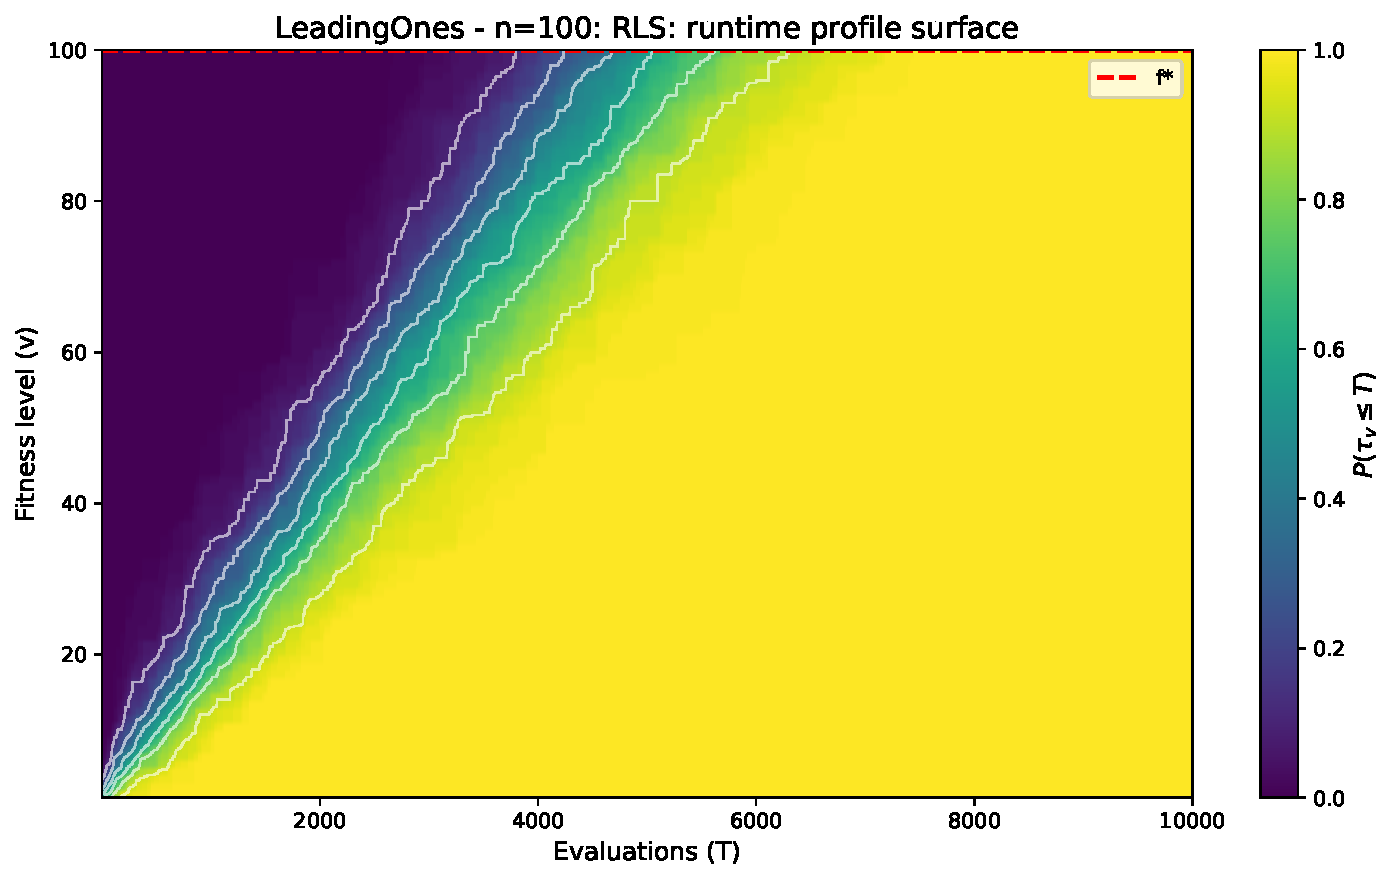
\includegraphics[width=\linewidth]{results/verification/inv_prof_surf_leadingones_RLS.pdf}
    \caption[\acrshort{rls} profile on
    \textsc{LeadingOnes}]{\acrshort{rls} for the \textsc{LeadingOnes} problem,
    with maximum budget 10\,000}
  \end{subfigure}
  \begin{subfigure}[t]{0.48\textwidth}
    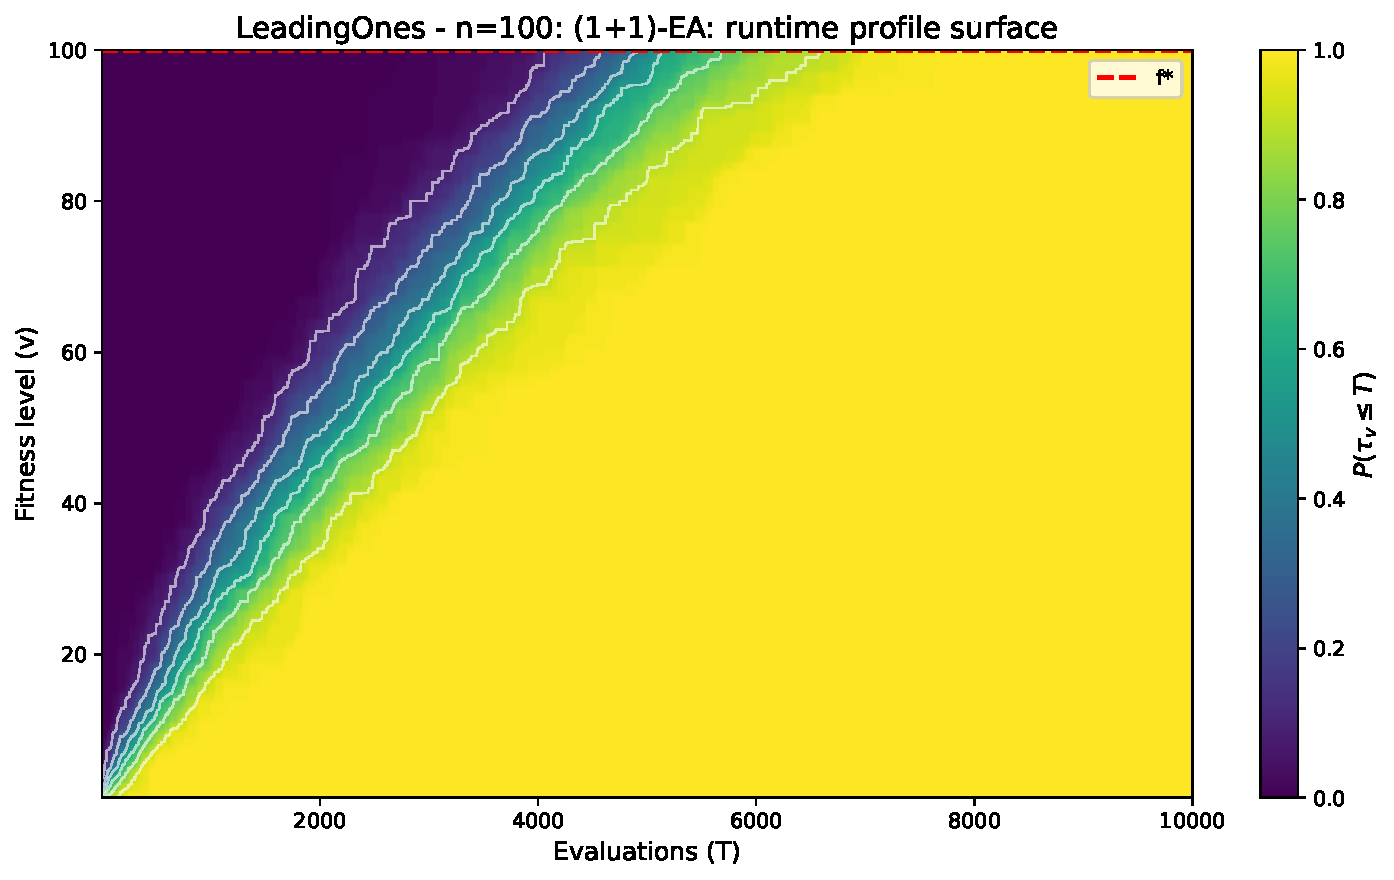
\includegraphics[width=\linewidth]{results/verification/inv_prof_surf_leadingones_(1+1)-EA.pdf}
    \caption[$(1+1)$-\acrshort{ea} profile on
    \textsc{LeadingOnes}]{$(1+1)$-\acrshort{ea} for the \textsc{LeadingOnes}
    problem, with maximum budget 10\,000}
  \end{subfigure}
  \caption[Inverse runtime profile plots]{Inverse runtime profile
    [$P(\tau_v \le T)$] plots for
  \acrshort{rls} and $(1+1)$-\acrshort{ea}}
  \label{fig:invprof}
\end{figure}
The inverse runtime profile surfaces in Figure~\ref{fig:invprof} show
the expected separation between
the two benchmark regimes. For \textsc{OneMax}, the saturation frontier is
compressed into the early part of the budget: low and intermediate fitness
levels satisfy $P(\tau_v \le T) \approx 1$ after only a few hundred
evaluations, and the contour near the optimum $f^\ast$ reaches high
probability well before the end of the displayed $T=1000$ window for both
\acrshort{rls} and the $(1+1)$-\acrshort{ea}. In contrast, the
\textsc{LeadingOnes} surfaces exhibit a broad diagonal transition band
across the full $T=10000$ range. The probability mass moves gradually from
low to high fitness levels, and the saturation frontier for $v=f^\ast$
appears only in the later part of the budget. This delayed frontier is
consistent with the sequential structure of \textsc{LeadingOnes}, where
progress depends on extending the correct prefix, and with the known
asymptotic contrast between the $\Theta(n \log n)$ optimization time of
\textsc{OneMax} and the $\Theta(n^2)$ behavior of
\textsc{LeadingOnes}. Thus, the inverse runtime profiles verify the profile
construction itself and preserve the qualitative finite-$n$ runtime ordering of
the underlying benchmark problems.

The verification result supports the use of profile-derived
$\mathbb{E}[\mathrm{CR}(T)]$ curves on integer-valued or explicitly
discretized fitness levels in the remaining evaluation suites. The same profile
construction provides a useful diagnostic reference in Suites~03 and~12, where
direct averaging is more susceptible to sampling noise because only $R=25$ runs
are available. For the real-valued NK landscapes, however, those profile
surfaces should be read as discretized approximations rather than exact
identities. Section~\ref{sec:results:synthesis} returns to this point by
relating the Suite~08 verification to the saturation frontiers observed in the
NK benchmark suites.
%
\section{Barrier Structure and Mutation Rate}
\label{sec:results:barrier}
\subsection{Suite 04: Trap --- Deception Width and Mutation Rate}
\label{sec:results:suite04}
\begin{figure}[!htbp]
  \centering
  \begin{subfigure}[t]{0.48\textwidth}
    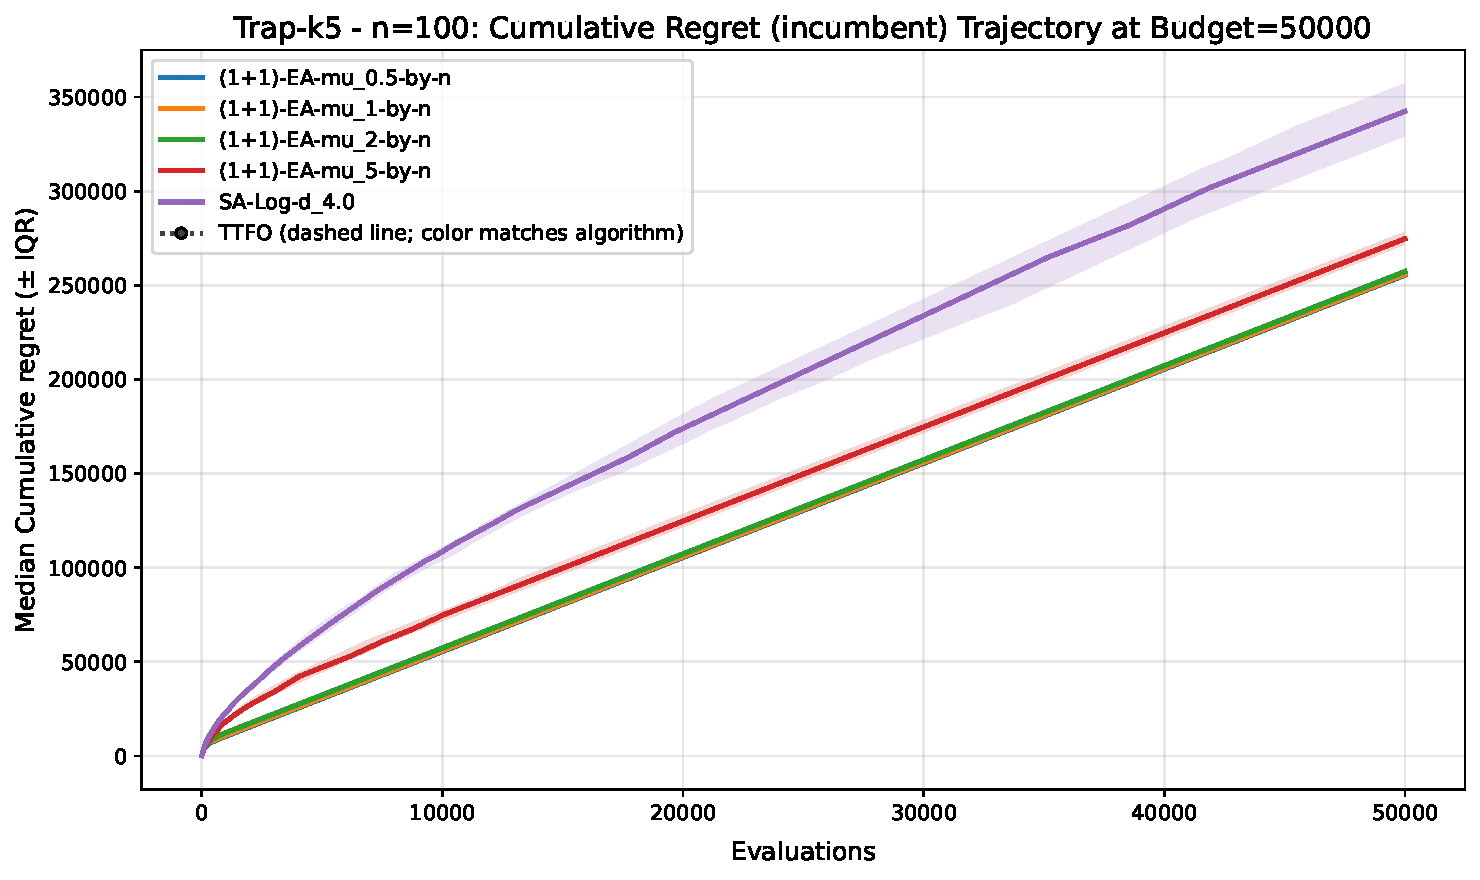
\includegraphics[width=\linewidth]{results/barrier_mut/trap/k5_history_regret_cumulative_best.pdf}
    \caption{\textsc{Trap}-$5$.}
    \label{fig:suite04-trap-k5-cr}
  \end{subfigure}
  \begin{subfigure}[t]{0.48\textwidth}
    \includegraphics[width=\linewidth]{results/barrier_mut/trap/k8_history_regret_cumulative_best.pdf}
    \caption{\textsc{Trap}-$8$.}
    \label{fig:suite04-trap-k8-cr}
  \end{subfigure}
  \begin{subfigure}[t]{0.48\textwidth}
    \includegraphics[width=\linewidth]{results/barrier_mut/trap/k10_history_regret_cumulative_best.pdf}
    \caption{\textsc{Trap}-$10$.}
    \label{fig:suite04-trap-k10-cr}
  \end{subfigure}
  \begin{subfigure}[t]{0.48\textwidth}
    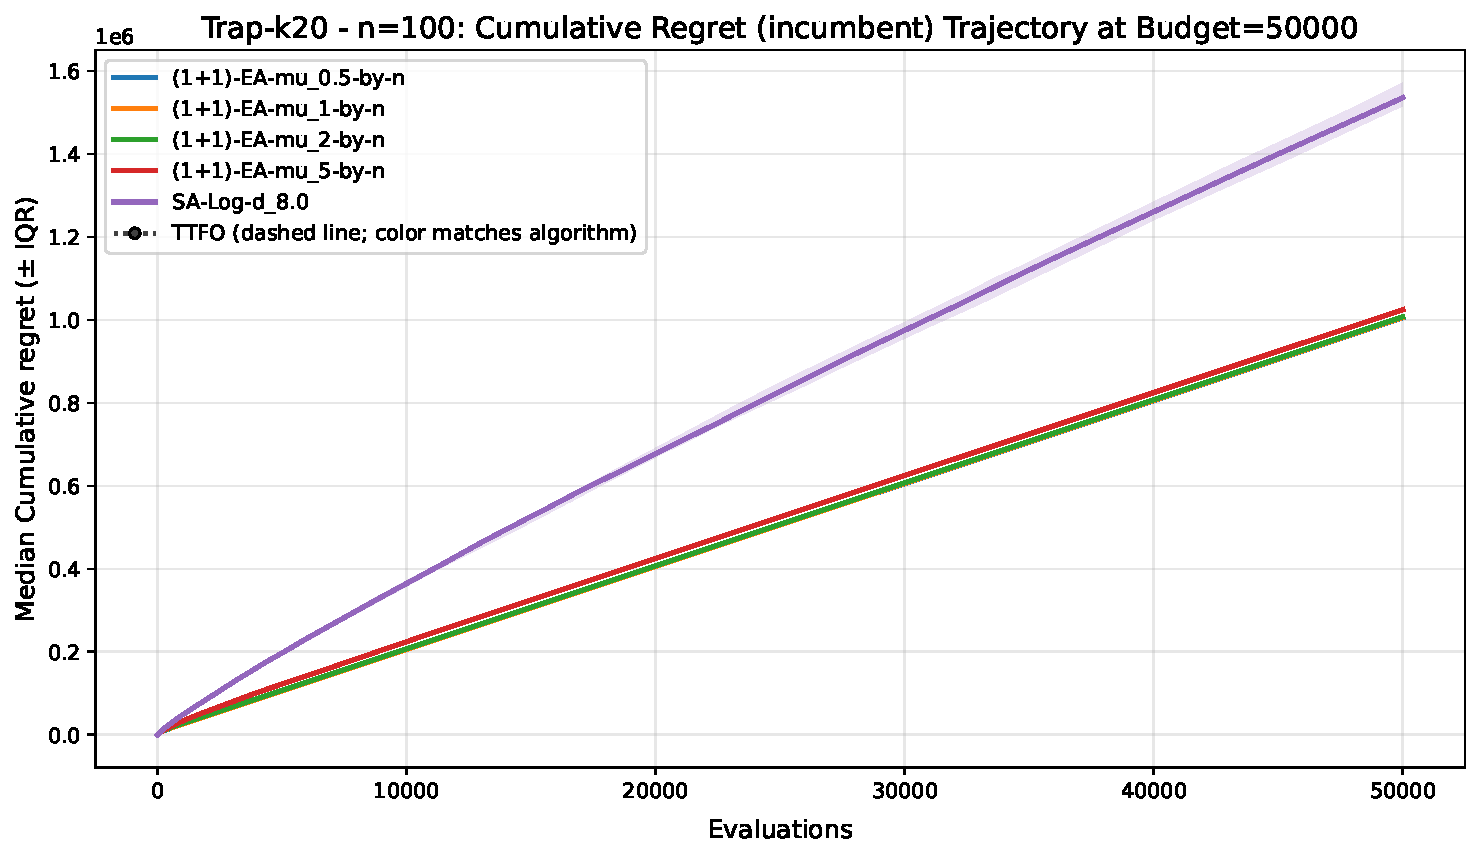
\includegraphics[width=\linewidth]{results/barrier_mut/trap/k20_history_regret_cumulative_best.pdf}
    \caption{\textsc{Trap}-$20$.}
    \label{fig:suite04-trap-k20-cr}
  \end{subfigure}
  \caption[Suite 04 Trap \acrshort{cr} trajectories]{Suite~04
    incumbent \acrshort{cr} trajectories on
    \textsc{Trap} as deception width increases. The trajectories remain
    non-convergent within budget, so the ramp height and slope carry the main
  diagnostic information.}
  \label{fig:suite04-trap-cr}
\end{figure}

\begin{figure}[!htbp]
  \centering
  \begin{subfigure}[t]{0.48\textwidth}
    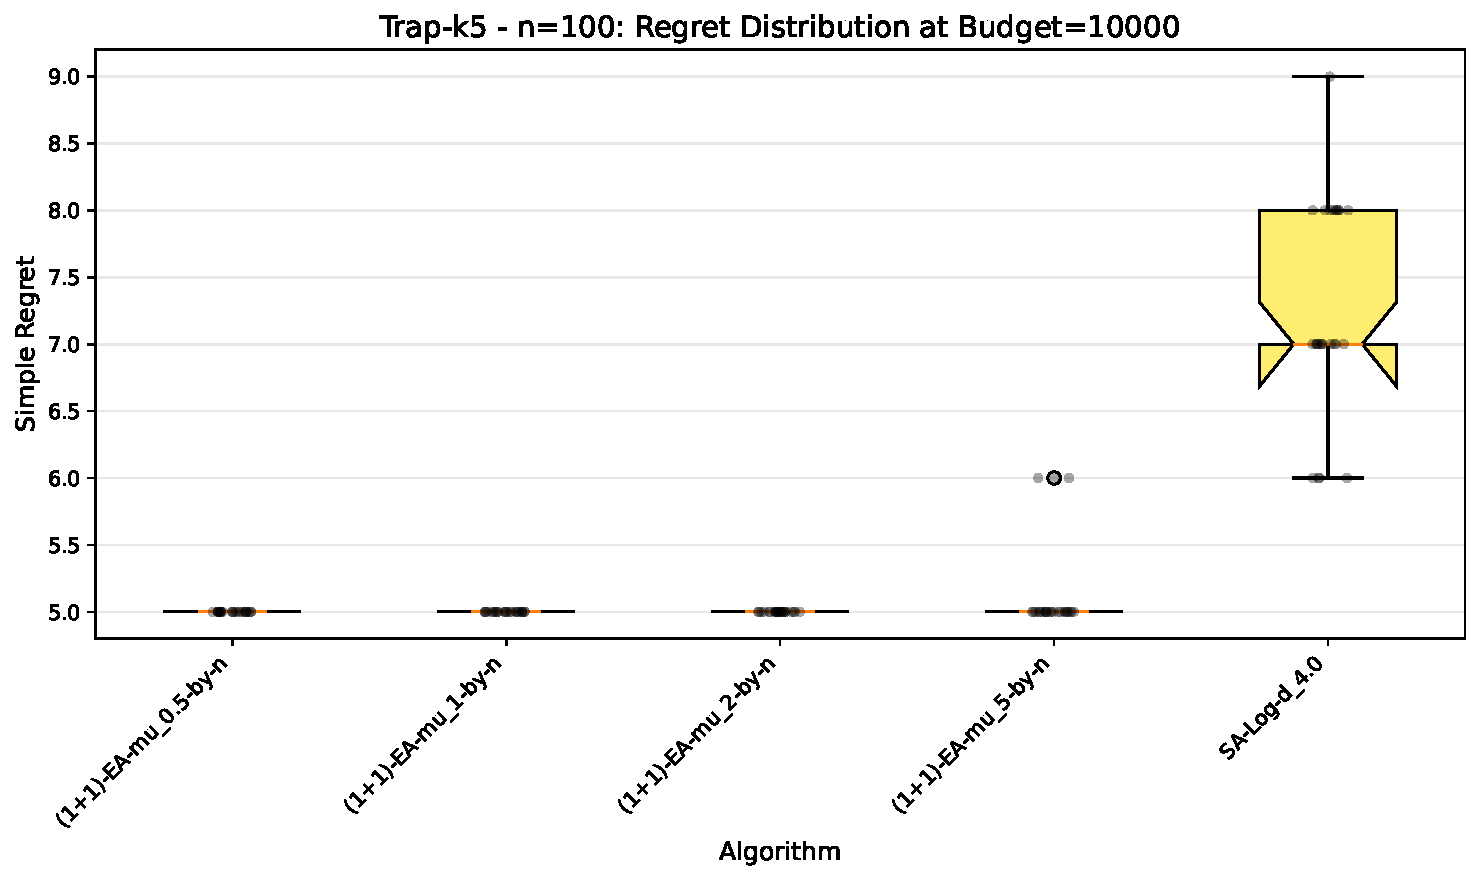
\includegraphics[width=\linewidth]{results/barrier_mut/trap/k5_regret_boxplot_b10000.pdf}
    \caption{\textsc{Trap}-$5$.}
    \label{fig:suite04-trap-k5-box}
  \end{subfigure}
  \begin{subfigure}[t]{0.48\textwidth}
    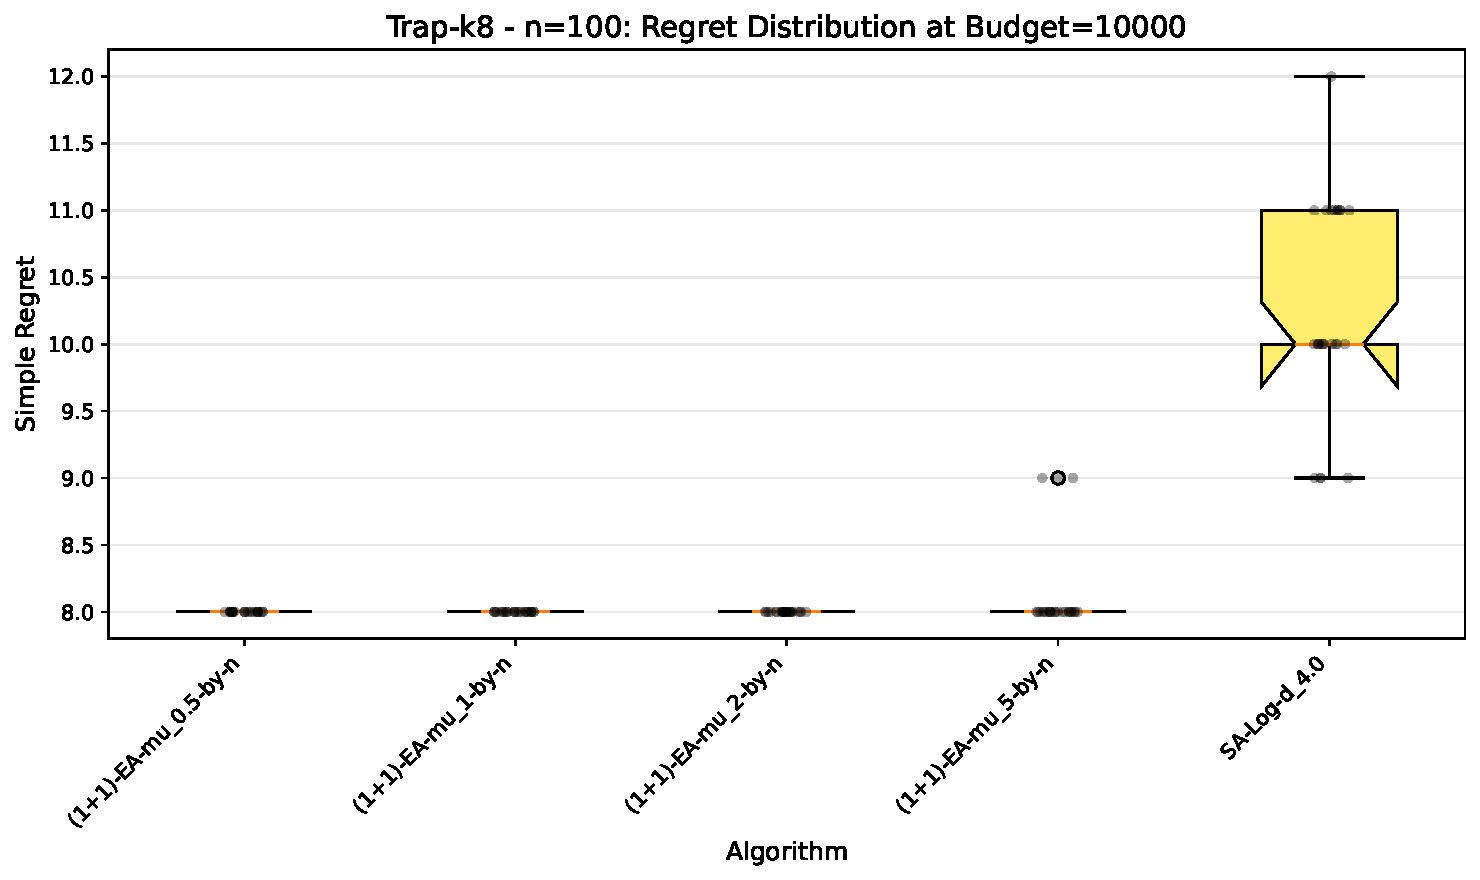
\includegraphics[width=\linewidth]{results/barrier_mut/trap/k8_regret_boxplot_b10000.pdf}
    \caption{\textsc{Trap}-$8$.}
    \label{fig:suite04-trap-k8-box}
  \end{subfigure}
  \begin{subfigure}[t]{0.48\textwidth}
    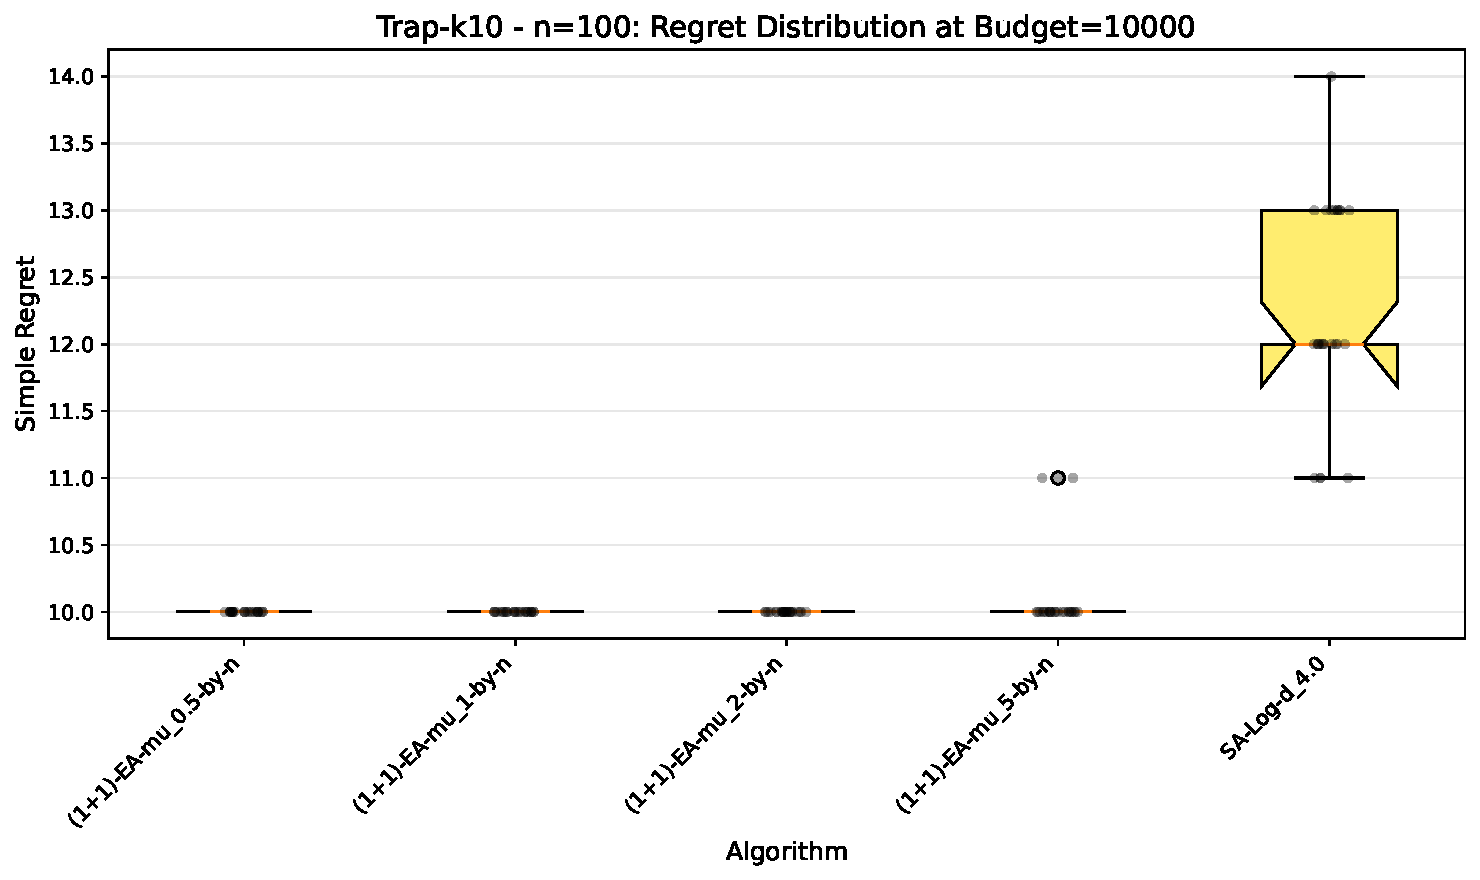
\includegraphics[width=\linewidth]{results/barrier_mut/trap/k10_regret_boxplot_b10000.pdf}
    \caption{\textsc{Trap}-$10$.}
    \label{fig:suite04-trap-k10-box}
  \end{subfigure}
  \begin{subfigure}[t]{0.48\textwidth}
    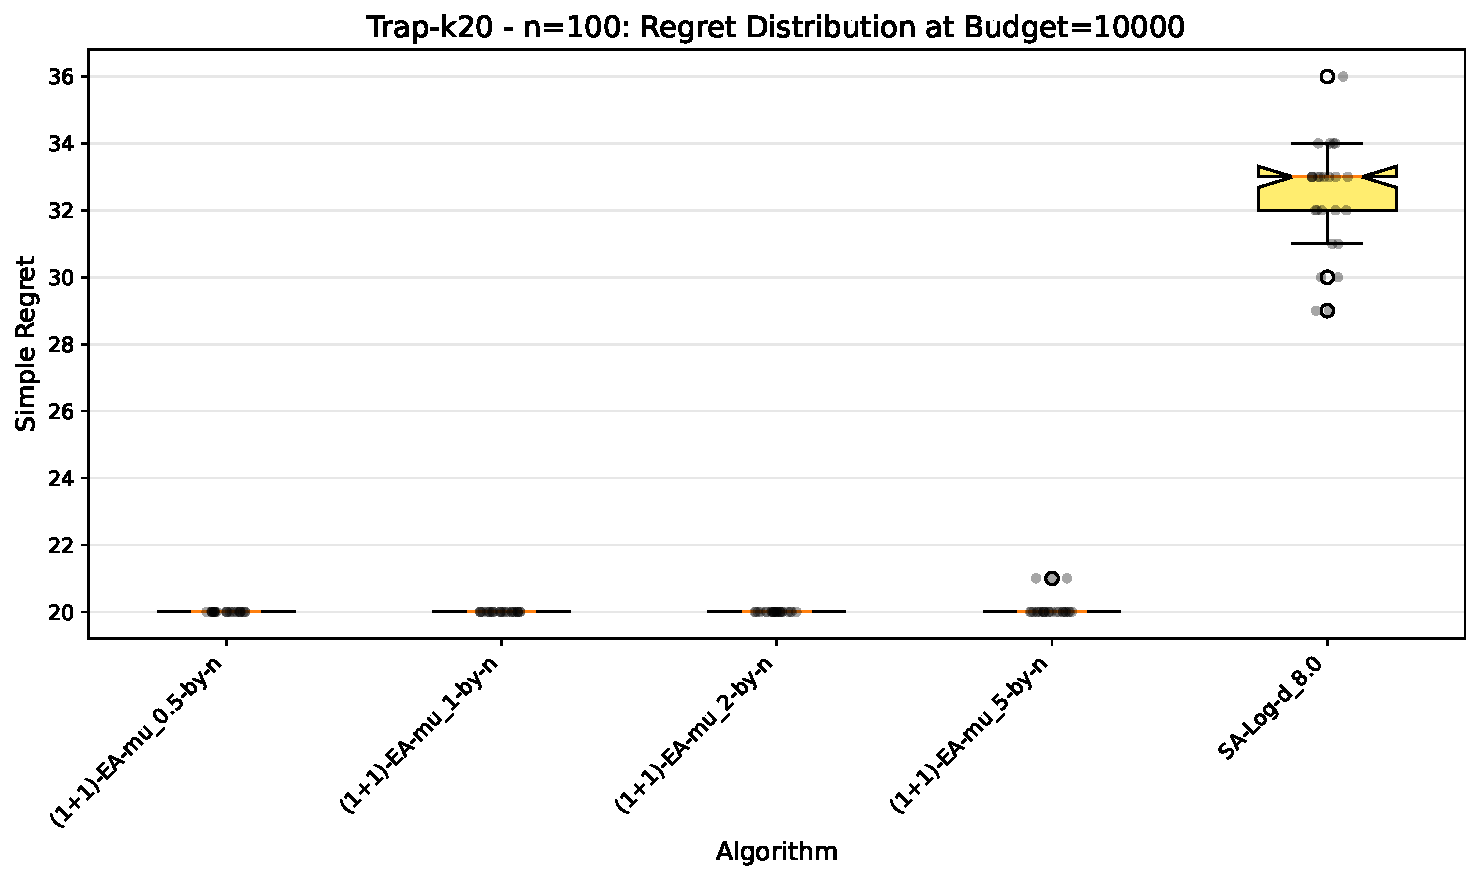
\includegraphics[width=\linewidth]{results/barrier_mut/trap/k20_regret_boxplot_b10000.pdf}
    \caption{\textsc{Trap}-$20$.}
    \label{fig:suite04-trap-k20-box}
  \end{subfigure}
  \caption[Suite 04 Trap regret distributions]{Suite~04 regret
    distributions at budget $10{,}000$ for
    increasing \textsc{Trap} widths. The boxplots summarize the end-of-budget
    regret separation between mutation rates and the simulated-annealing
  schedule.}
  \label{fig:suite04-trap-box}
\end{figure}

Across Trap instances, \acrshort{sa} does not reach the global optimum within
the allotted budget, matching the failure of the \acrshort{ea} variants and
indicating that the tested temperature schedule is insufficient to
traverse the deceptive gradient (Figure~\ref{fig:suite04-trap-box}).
Its higher exploratory mobility
instead produces consistently larger incumbent cumulative regret: for
$k \neq 20$, the separation between the \acrshort{sa} trajectory and
the \acrshort{ea}
trajectories becomes slightly visible as $k$ grows, although the
eventual stabilized regret slopes remain broadly similar across
algorithms and deception widths.
The $d=8.0$ override on Trap-$k20$
does not alter this qualitative conclusion; it still fails to
converge within the budget and its \acrshort{cr} remains
substantially displaced from the \acrshort{ea} curves, again reflecting
exploration rather than successful escape. Thus, Suite~04 provides a
negative but informative result: increased exploration raises
cumulative regret without guaranteeing optimization success on the fully
deceptive Trap landscape (Figures~\ref{fig:suite04-trap-cr}
and~\ref{fig:suite04-trap-box}).

\subsection{Suites 05 and 09: Jump --- Mutation Rate and
Matched-Budget Reference}
\label{sec:results:suite05}
\begin{figure}[!htbp]
  \centering
  \begin{subfigure}[t]{0.48\textwidth}
    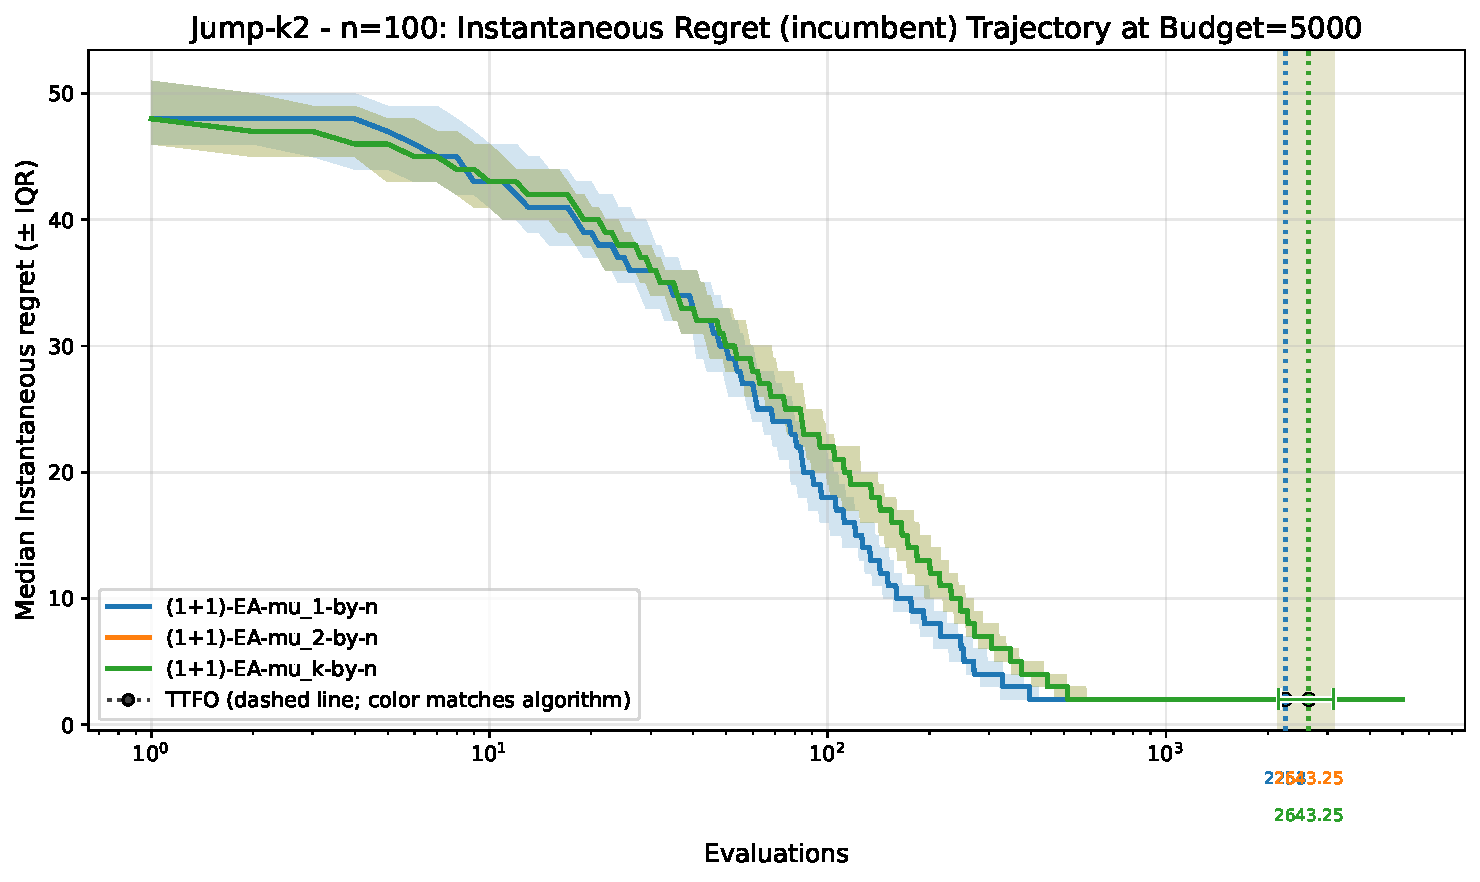
\includegraphics[width=\linewidth]{results/barrier_mut/jump/k2-history_regret_instantaneous_best.pdf}
    \caption{\textsc{Jump}-$2$.}
  \end{subfigure}
  \begin{subfigure}[t]{0.48\textwidth}
    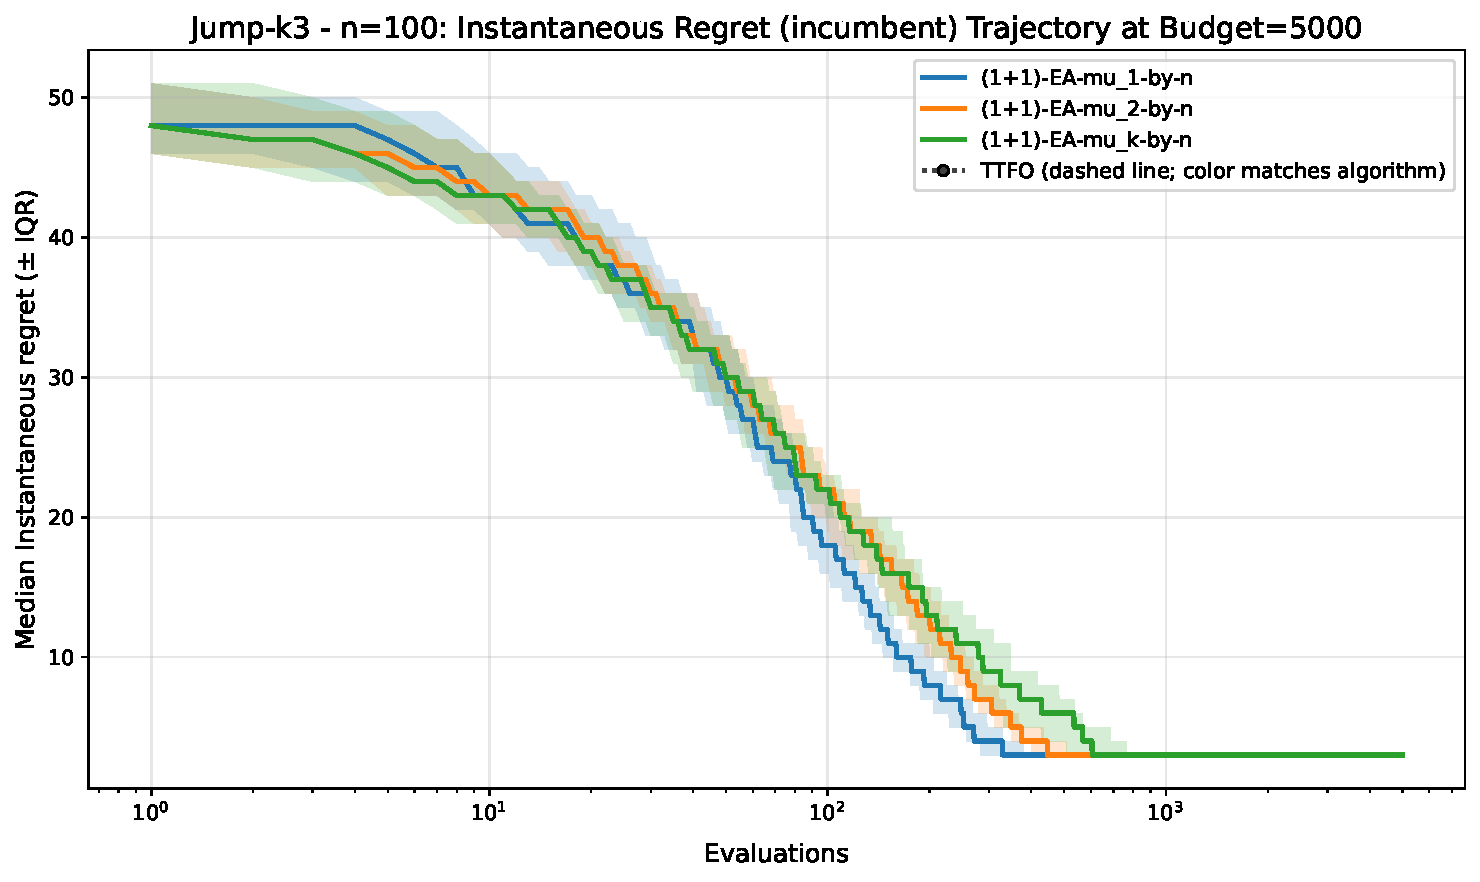
\includegraphics[width=\linewidth]{results/barrier_mut/jump/k3-history_regret_instantaneous_best.pdf}
    \caption{\textsc{Jump}-$3$.}
  \end{subfigure}
  \caption[Suite 05 small-jump instantaneous regret]{Suite~05
    incumbent \acrshort{ir} trajectories for small
    jump widths. The plateau height identifies the residual barrier after the
  local optimum is reached.}
  \label{fig:jumpinst-small}
\end{figure}

\begin{figure}[!htbp]
  \centering
  \begin{subfigure}[t]{0.48\textwidth}
    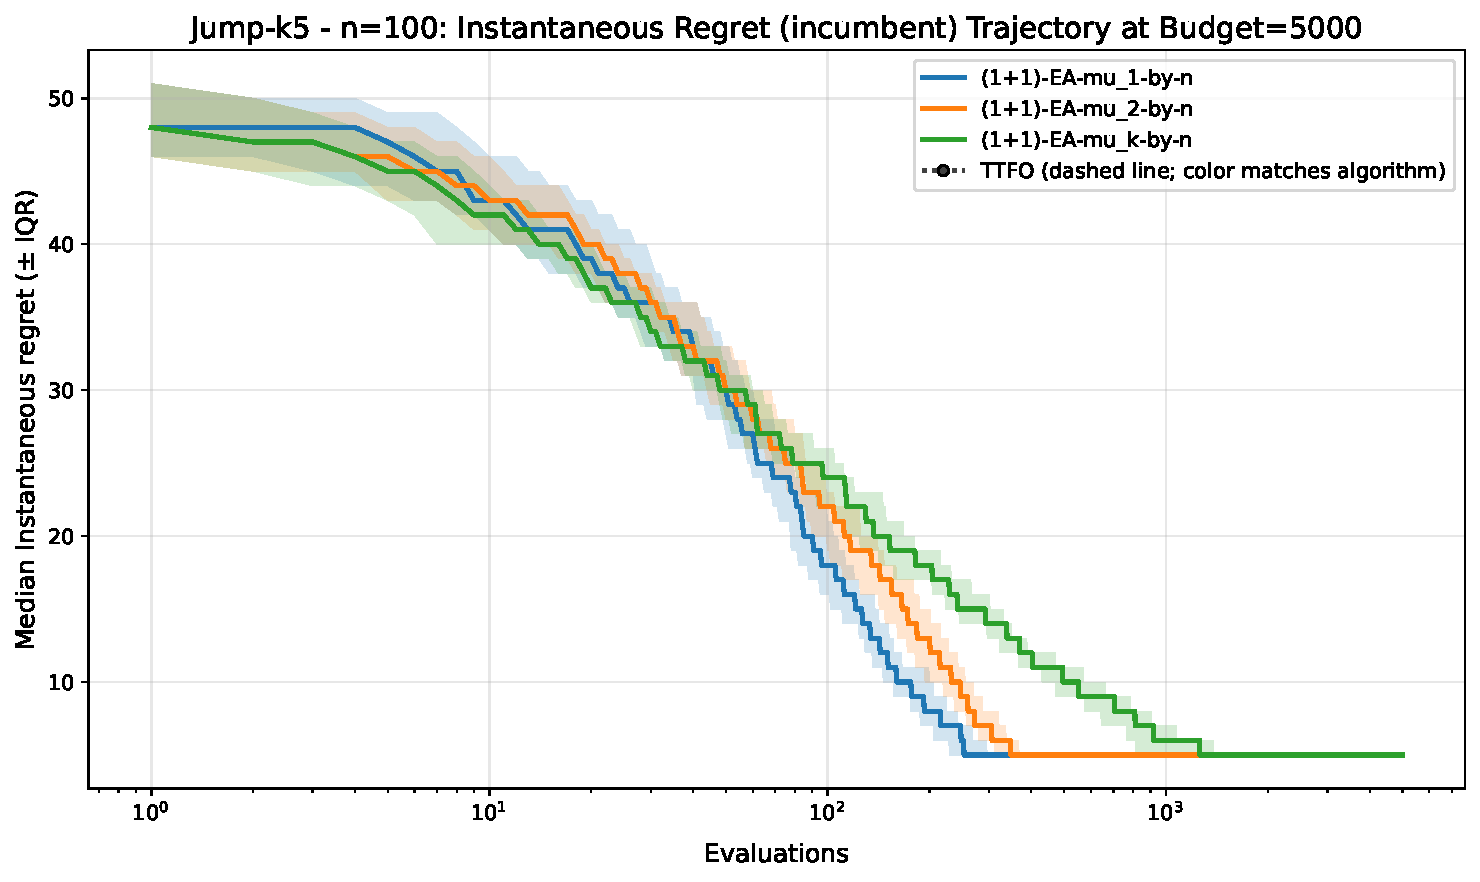
\includegraphics[width=\linewidth]{results/barrier_mut/jump/k5-history_regret_instantaneous_best.pdf}
    \caption{\textsc{Jump}-$5$.}
  \end{subfigure}
  \begin{subfigure}[t]{0.48\textwidth}
    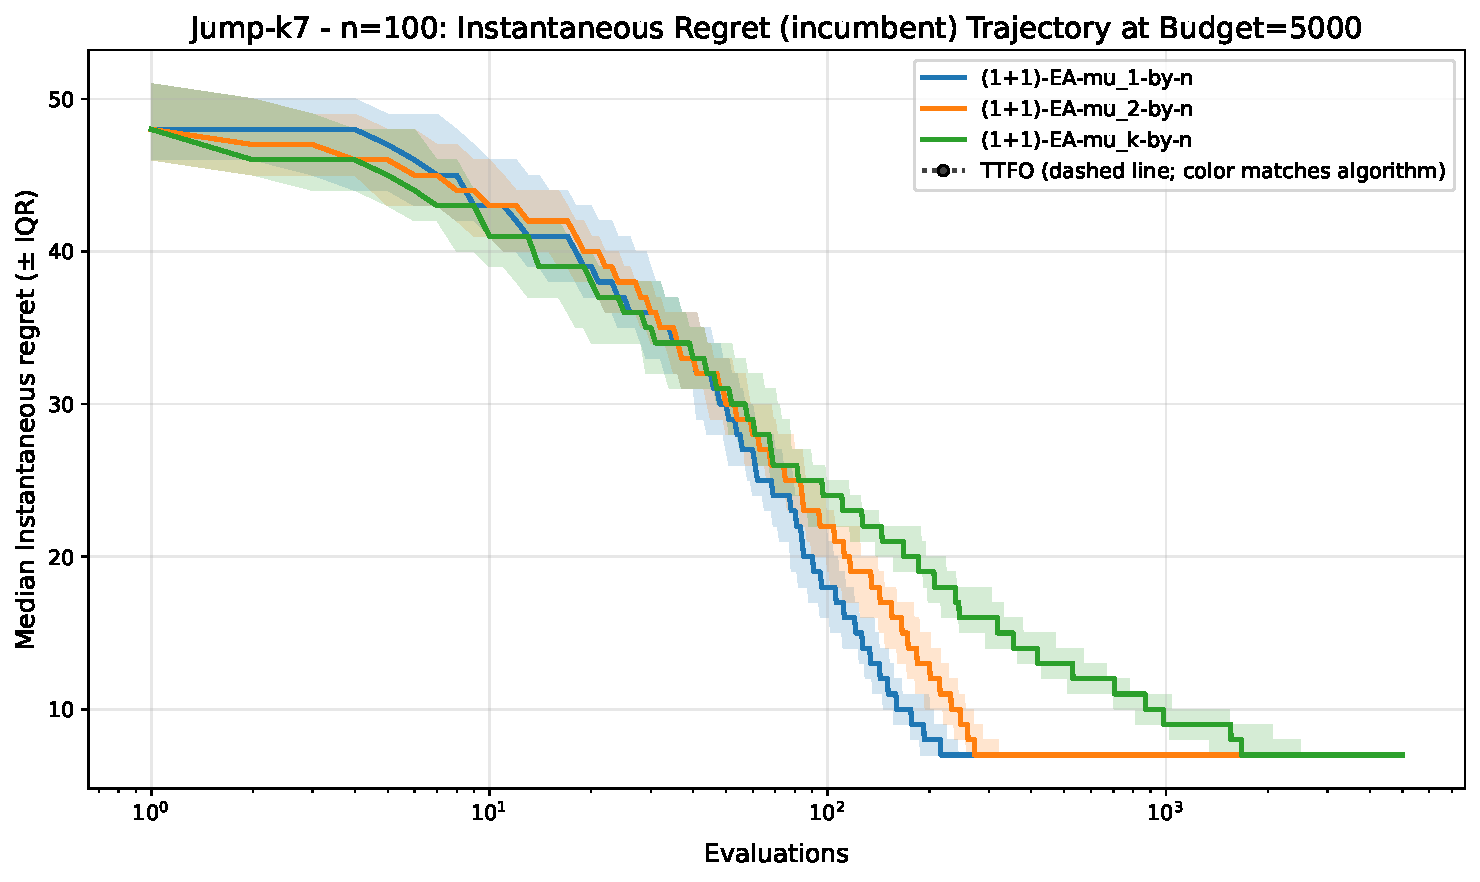
\includegraphics[width=\linewidth]{results/barrier_mut/jump/k7-history_regret_instantaneous_best.pdf}
    \caption{\textsc{Jump}-$7$.}
  \end{subfigure}
  \begin{subfigure}[t]{0.80\textwidth}
    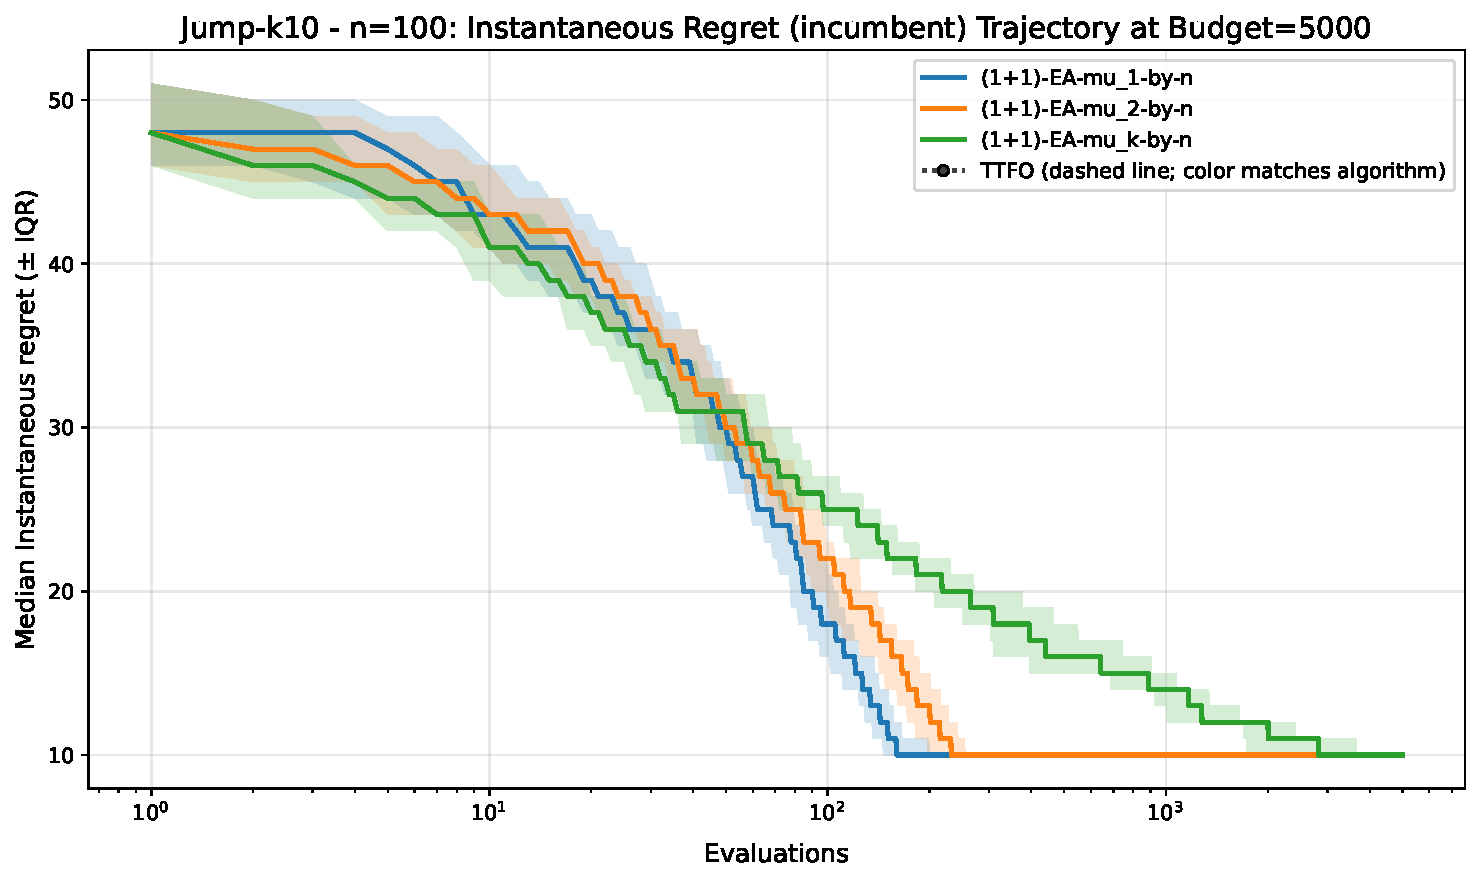
\includegraphics[width=\linewidth]{results/barrier_mut/jump/k10-history_regret_instantaneous_best.pdf}
    \caption{\textsc{Jump}-$10$.}
  \end{subfigure}
  \caption[Suite 05 Jump instantaneous regret]{Suite~05 incumbent
    \acrshort{ir} trajectories for
    \textsc{Jump}-$k$, $k\in\{5,7,10\}$. The trajectories descend into a
    width-dependent plateau whose height equals the remaining fitness gap to
  the optimum.}
  \label{fig:jumpinst}
\end{figure}
Figures~\ref{fig:jumpinst-small} and~\ref{fig:jumpinst} depict the incumbent, instantaneous regret
curves for Jump-$k$, $k \in \{2,3,5,7,10\}$.
The instantaneous incumbent-regret trajectories show two
distinct phases: an initial descent toward the local optimum, followed by a
flat plateau at regret $k$ once the search reaches Hamming weight $n-k$.
On linear axes, increasing the mutation rate delays this settling phase:
higher-rate variants spend longer at intermediate incumbent-regret levels
before collapsing onto the plateau. Thus, the plateau height remains
structurally determined by the jump width, while the mutation rate primarily
changes the transient path into the plateau.

\begin{figure}[!htbp]
  \centering
  \begin{subfigure}[t]{0.48\textwidth}
    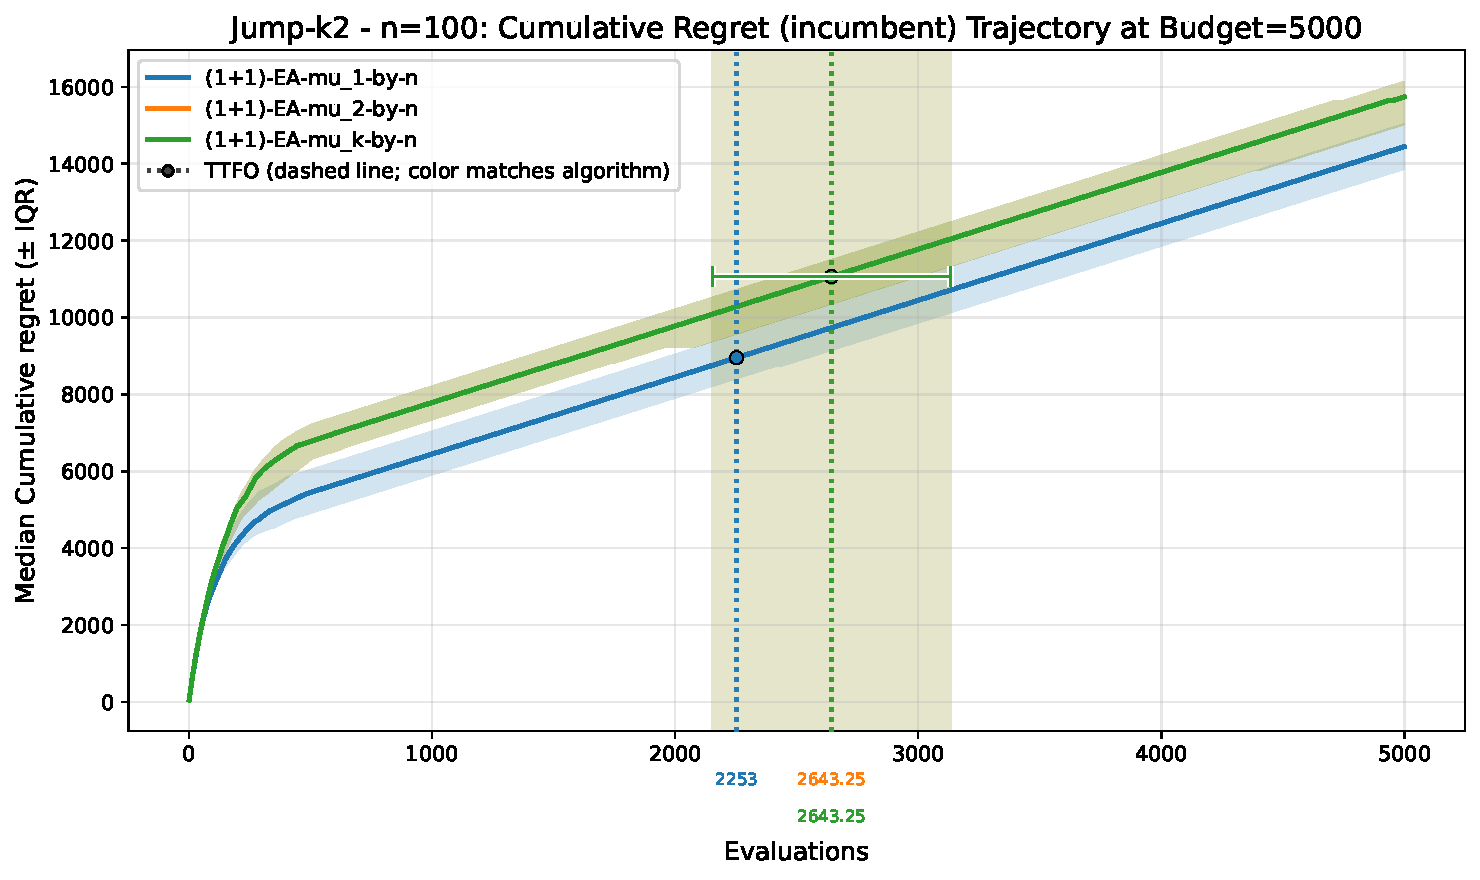
\includegraphics[width=\linewidth]{results/barrier_mut/jump/k2-history_regret_cumulative_best.pdf}
    \caption{\textsc{Jump}-$2$.}
    \label{fig:suite05-jump-k2-cr}
  \end{subfigure}
  \begin{subfigure}[t]{0.48\textwidth}
    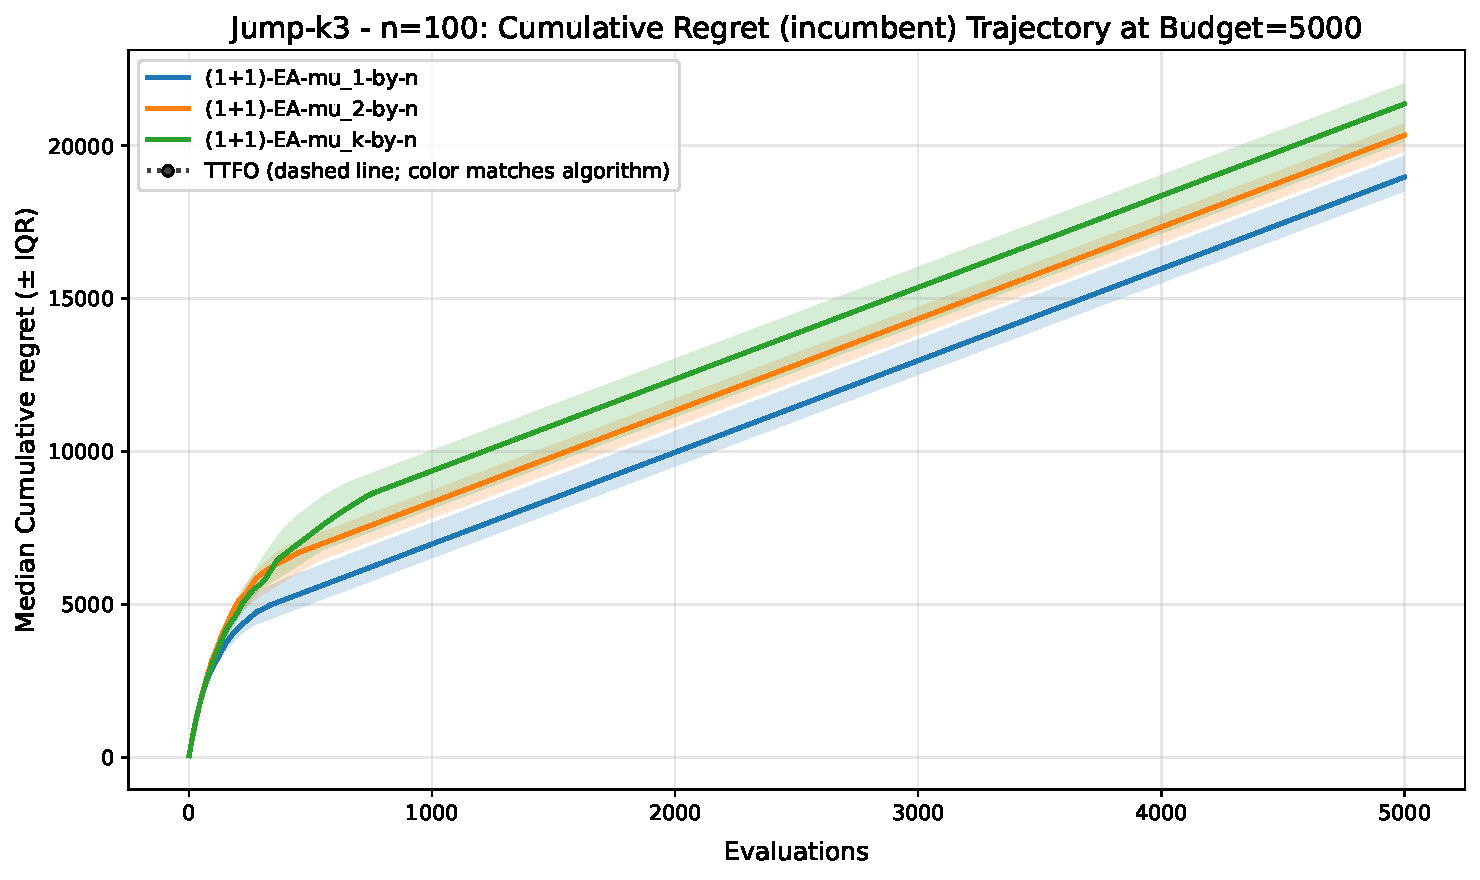
\includegraphics[width=\linewidth]{results/barrier_mut/jump/k3-history_regret_cumulative_best.pdf}
    \caption{\textsc{Jump}-$3$.}
    \label{fig:suite05-jump-k3-cr}
  \end{subfigure}
  \begin{subfigure}[t]{0.48\textwidth}
    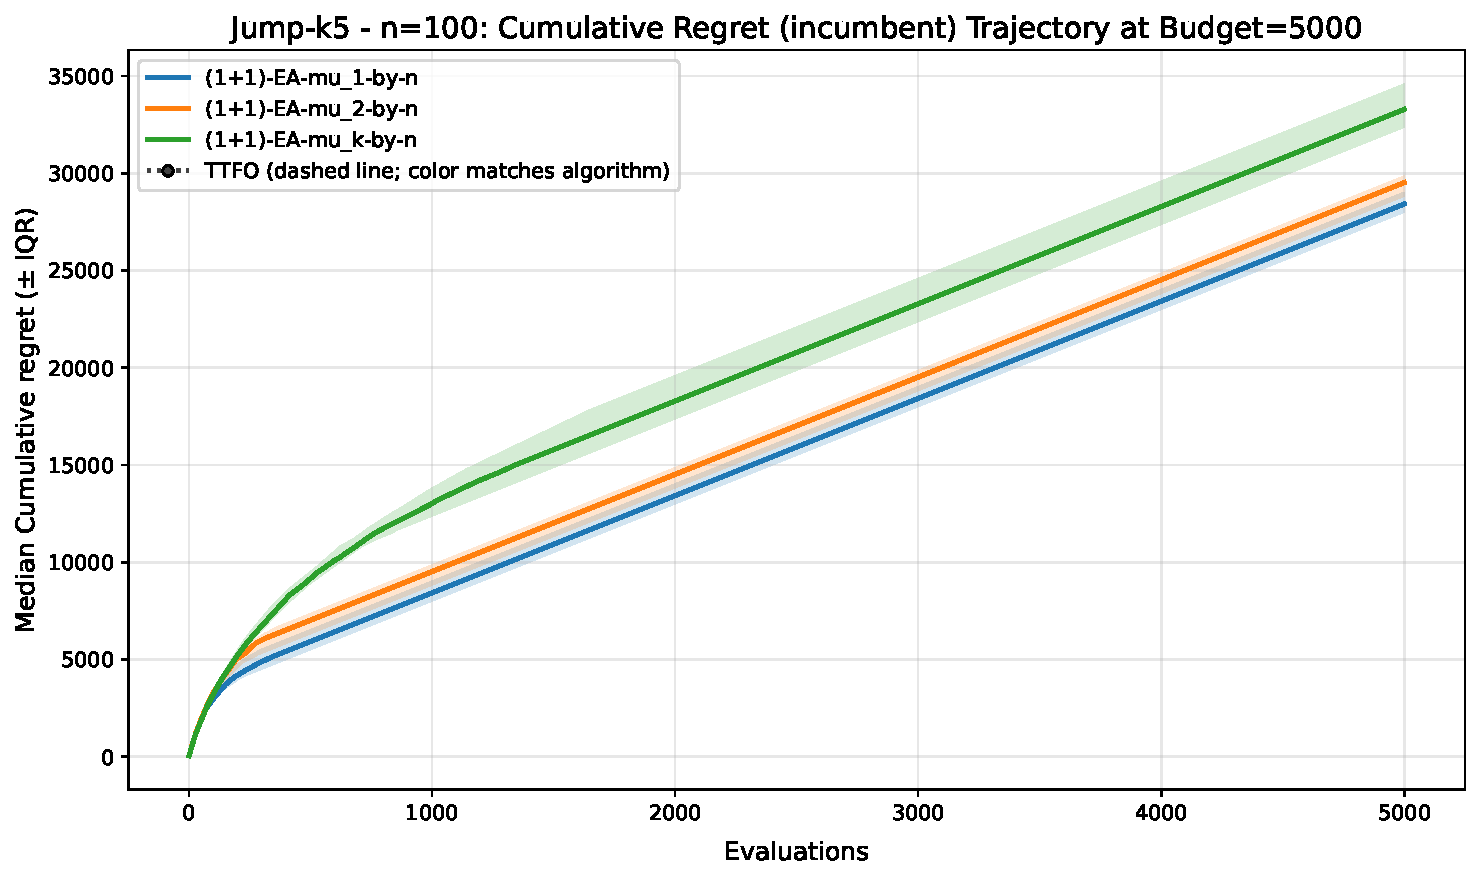
\includegraphics[width=\linewidth]{results/barrier_mut/jump/k5-history_regret_cumulative_best.pdf}
    \caption{\textsc{Jump}-$5$.}
    \label{fig:suite05-jump-k5-cr}
  \end{subfigure}
  \begin{subfigure}[t]{0.48\textwidth}
    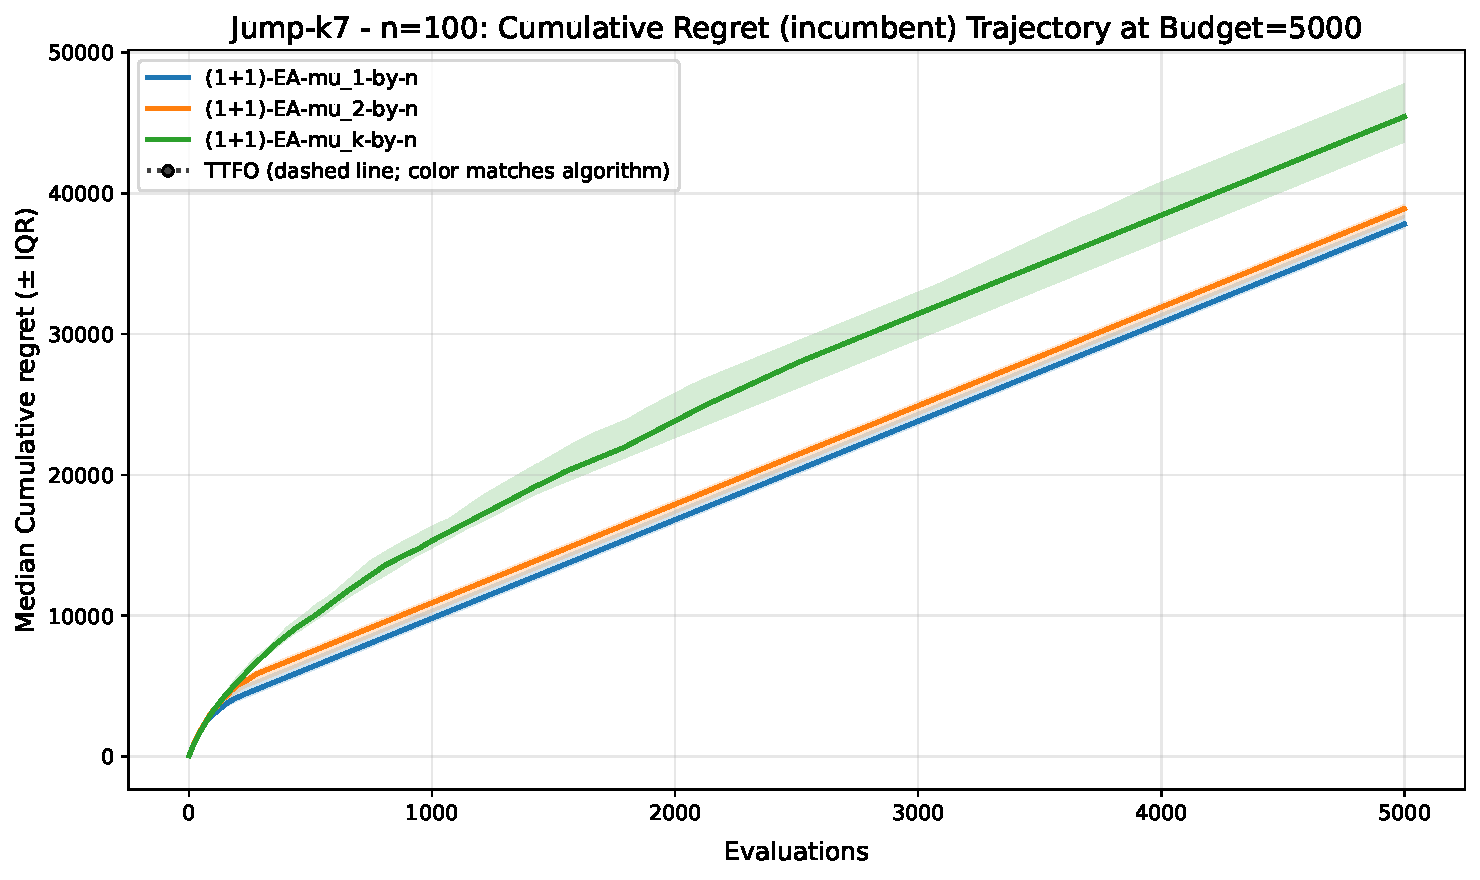
\includegraphics[width=\linewidth]{results/barrier_mut/jump/k7-history_regret_cumulative_best.pdf}
    \caption{\textsc{Jump}-$7$.}
    \label{fig:suite05-jump-k7-cr}
  \end{subfigure}
  \begin{subfigure}[t]{0.80\textwidth}
    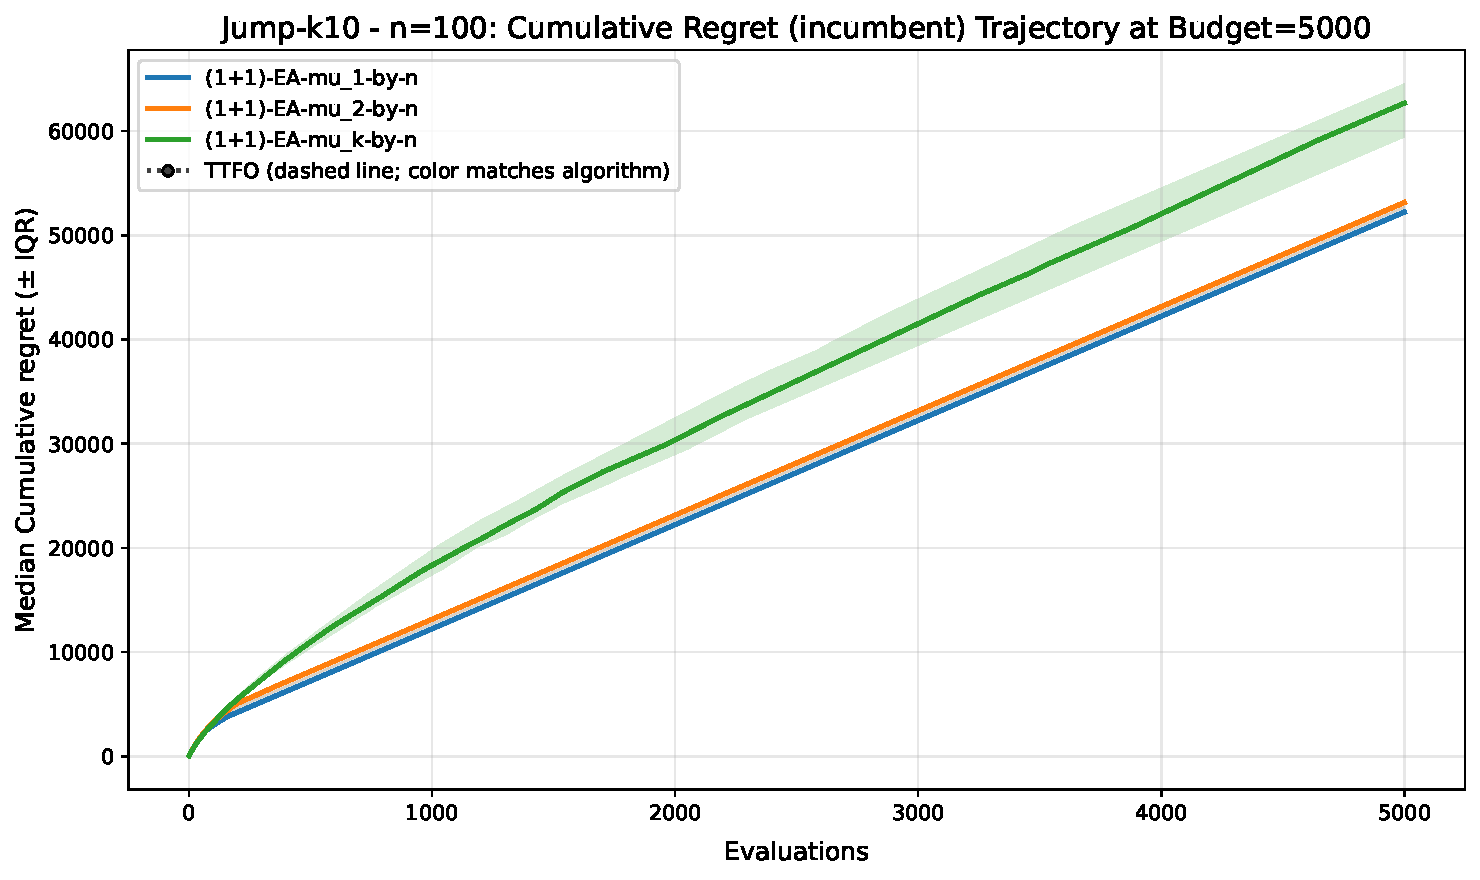
\includegraphics[width=\linewidth]{results/barrier_mut/jump/k10-history_regret_cumulative_best.pdf}
    \caption{\textsc{Jump}-$10$.}
    \label{fig:suite05-jump-k10-cr}
  \end{subfigure}
  \caption[Suite 05 Jump cumulative regret]{Suite~05 incumbent
    \acrshort{cr} trajectories on
    \textsc{Jump} as the jump width increases. After the initial descent, the
    trapped phase appears as an approximately linear ramp whose slope is set by
  the incumbent regret plateau.}
  \label{fig:suite05-jump-cr}
\end{figure}

\begin{figure}[!htbp]
  \centering
  \begin{subfigure}[t]{0.48\textwidth}
    
\includegraphics[width=\linewidth]{results/barrier_mut/jump_plateau/k2-history_regret_cumulative_best.pdf}
    \caption{Matched-budget cumulative regret.}
    \label{fig:suite09-jump-k2-cr}
  \end{subfigure}
  \begin{subfigure}[t]{0.48\textwidth}
    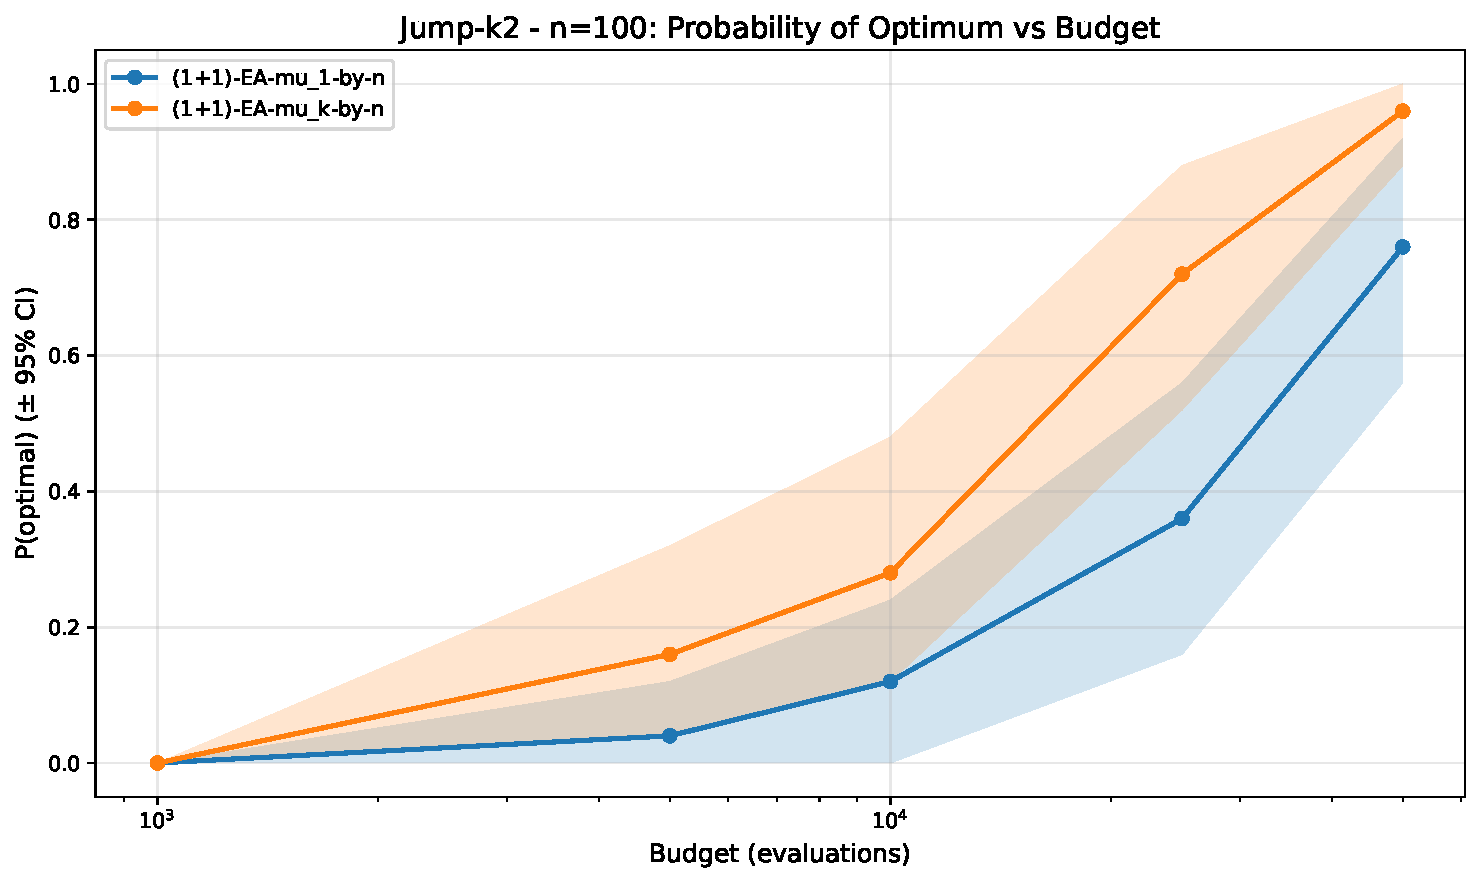
\includegraphics[width=\linewidth]{results/barrier_mut/jump_plateau/k2-convergence_probability.pdf}
    \caption{Matched-budget convergence probability.}
    \label{fig:suite09-jump-k2-cdp}
  \end{subfigure}
  \caption[Suite 09 matched-budget Jump reference]{Suite~09
    matched-budget reference for \textsc{Jump}-$2$.
    Cumulative regret records the cost of the trapped phase, while convergence
  probability records only whether the optimum has been hit by each budget.}
  \label{fig:suite09-jump-k2}
\end{figure}
The adaptive $k/n$ mutation rate increasingly separates from the fixed-rate
\acrshort{cr} curves as $k$ grows, a pattern visible both in Suite~05 and
in the matched-budget Suite~09 reference. In Suite~05, the $k/n$ variant
coincides with the fixed $2/n$ rate at $k=2$; for larger $k$, the longer
residence at intermediate incumbent-regret levels before the regret-$k$ plateau
produces a larger \acrshort{cr} gap; see
Figures~\ref{fig:suite05-jump-cr} and~\ref{fig:suite09-jump-k2}. This
also shows why mean simple regret and convergence probability can be
misleading at high budgets: they record the eventual plateau or success state,
but not the accumulated cost of reaching it.

\subsection{Suite 06: Plateau --- Neutral Walk and Mutation Rate}
\label{sec:results:suite06}
\begin{figure}[!htbp]
  \centering
  \begin{subfigure}[t]{0.48\textwidth}
    
\includegraphics[width=\linewidth]{results/barrier_mut/plateau/k2-history_regret_instantaneous_best.pdf}
    \caption{\textsc{Plateau}-$2$ instantaneous regret.}
    \label{fig:suite06-plateau-k2-ir}
  \end{subfigure}
  \begin{subfigure}[t]{0.48\textwidth}
    
\includegraphics[width=\linewidth]{results/barrier_mut/plateau/k2-history_regret_cumulative_best.pdf}
    \caption{\textsc{Plateau}-$2$ cumulative regret.}
    \label{fig:suite06-plateau-k2-cr}
  \end{subfigure}
  \begin{subfigure}[t]{0.48\textwidth}
    
\includegraphics[width=\linewidth]{results/barrier_mut/jump_plateau/k2-history_regret_cumulative_best.pdf}
    \caption{\textsc{Jump}-$2$ cumulative regret.}
    \label{fig:suite09-jump-k2-cr-plateau-ref}
  \end{subfigure}
  \begin{subfigure}[t]{0.48\textwidth}
    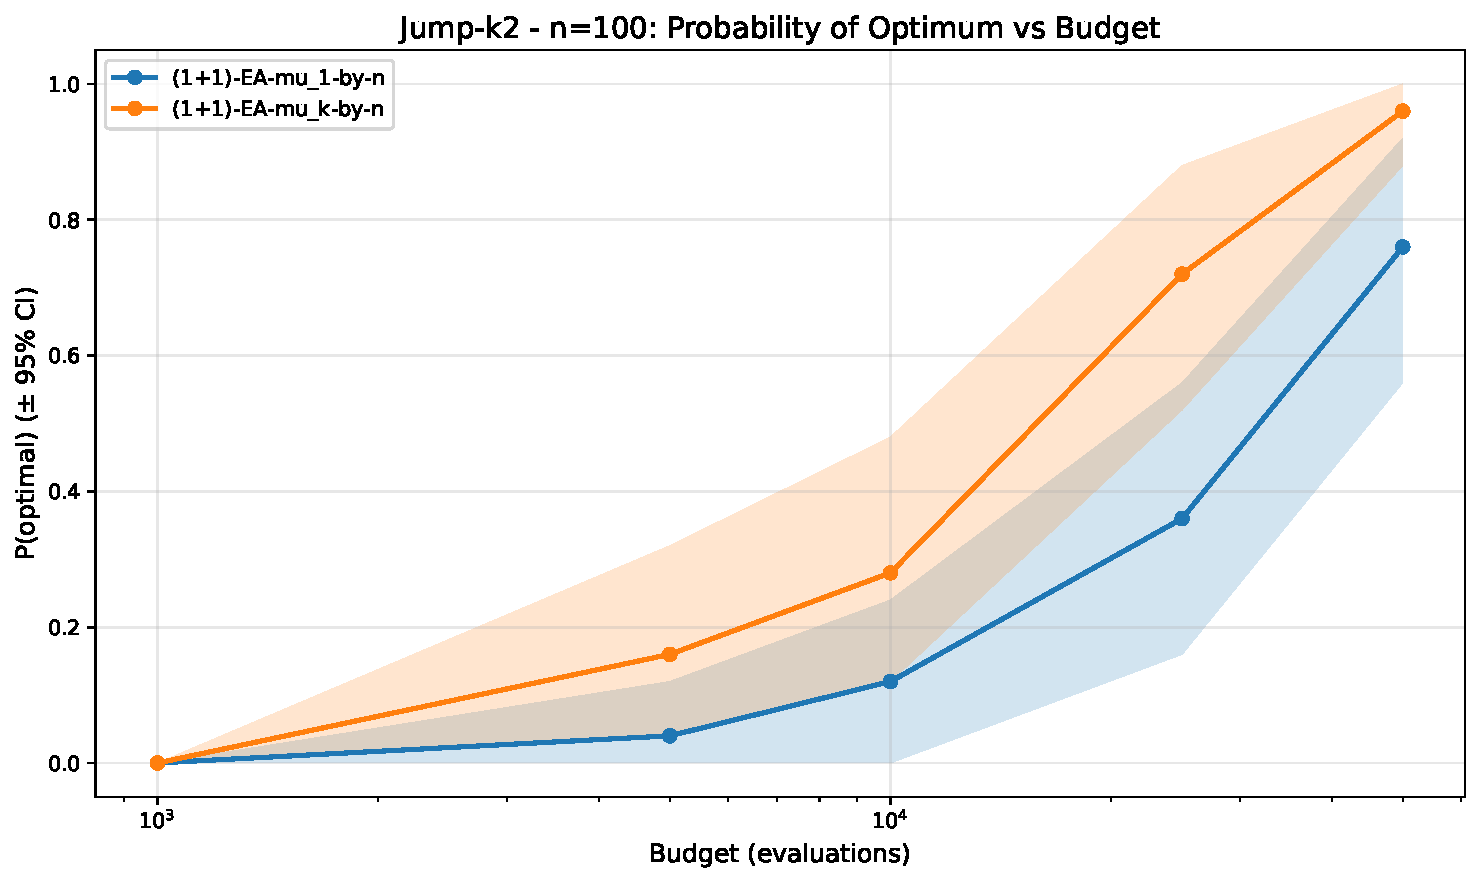
\includegraphics[width=\linewidth]{results/barrier_mut/jump_plateau/k2-convergence_probability.pdf}
    \caption{\textsc{Jump}-$2$ convergence probability.}
    \label{fig:suite09-jump-k2-cdp-plateau-ref}
  \end{subfigure}
  \caption[Matched Plateau and Jump comparison]{Matched $k=2$
    comparison between the neutral-walk
    \textsc{Plateau} landscape and the fitness-valley \textsc{Jump}
    landscape. Plateau and Jump differ most clearly in the early
  \acrshort{ir} descent and in the median \acrshort{cr} recovery.}
  \label{fig:suite06-plateau-jump-k2}
\end{figure}

\begin{figure}[!htbp]
  \centering
  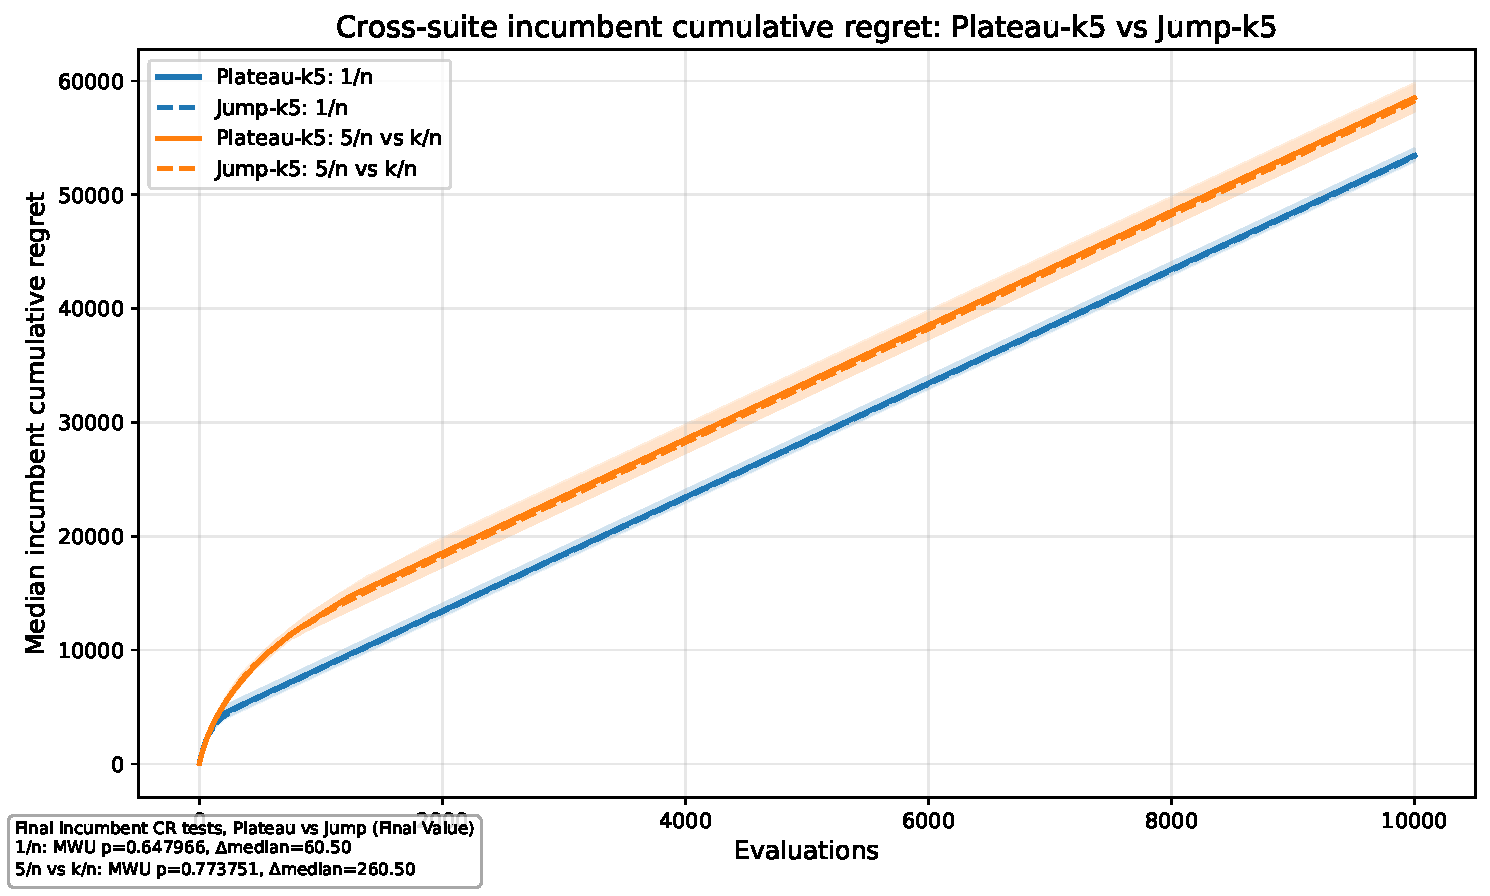
\includegraphics[width=0.80\textwidth]{results/barrier_mut/plateau_jump/plateau_vs_jump_k5_b10000.pdf}
  \caption[Plateau and Jump regret distributions]{Budget-$10{,}000$
    comparison of \textsc{Plateau}-$5$ and
    \textsc{Jump}-$5$ regret distributions. At this width the neutral-walk and
    fitness-valley mechanisms are much less visually separable than at
  $k=2$.}
  \label{fig:suite06-plateau-jump-k5}
\end{figure}

The Plateau results are most informative when compared cross-suite against the
matched-budget Jump reference in Suite~09, since Suite~06 does not
contain Jump curves.
At $k=2$, the incumbent \acrshort{cr} trajectories are visually distinct:
Plateau-$2$ shows faster median recovery for several EA variants, and under the
$10{,}000$-evaluation budget some median curves reach zero incumbent
instantaneous regret (Figure~\ref{fig:suite06-plateau-k2-ir}),
indicating convergence to the global optimum
in the \acrshort{cr} trajectory
(Figure~\ref{fig:suite06-plateau-k2-cr}). This contrasts with
Jump-$2$ at the same budget, where optima are
sampled in some runs, but the median trajectory does not converge
Figures~\ref{fig:suite09-jump-k2-cr-plateau-ref}
and~\ref{fig:suite09-jump-k2-cdp-plateau-ref}. At $k=5$, however, the
distinction largely disappears:
the Plateau and Jump \acrshort{cr} curves are similar both in shape and in
magnitude (Figure~\ref{fig:suite06-plateau-jump-k5}). Thus, the
neutral-walk mechanism is
clearly separable from Jump at small $k$, but becomes empirically harder to
distinguish from a fitness-valley barrier as $k$ increases.

Thus, Suite~06 exposes a boundary of the \acrshort{cr} diagnostic:
\acrshort{cr} is not meant to distinguish the landscape identity, it just
hints at the realized optimization cost.
When Plateau and Jump differ strongly, as at $k=2$, their
incumbent \acrshort{cr} trajectories separate; when their induced search
costs are similar, as at $k=5$, the curves may overlap despite different
underlying mechanisms. Cumulative regret should therefore be read as an
algorithm--problem trajectory diagnostic.

\subsection{Suite 10: Barrier Archetype Comparison at $k=5$}
\label{sec:results:suite10}

Suite~10 fixes $k=5$ across \textsc{Jump}, \textsc{Trap}, and
\textsc{Plateau} because endpoint convergence is deliberately absent:
none of the tested $(1+1)$-\acrshort{ea} mutation-rate variants reaches
the global optimum within the available budget on any of the three
problems. Rather than reproduce three identical zero-convergence panels,
Figure~\ref{fig:suite10-regret-boxplot} shows the corresponding budget-level
regret distribution for the representative \textsc{Jump}-$5$ case.
The comparison therefore queries how different barrier mechanisms are
reflected in the regret trajectories when \acrshort{ttfo} provides no
usable samples.

\begin{figure}[!htbp]
  \centering
  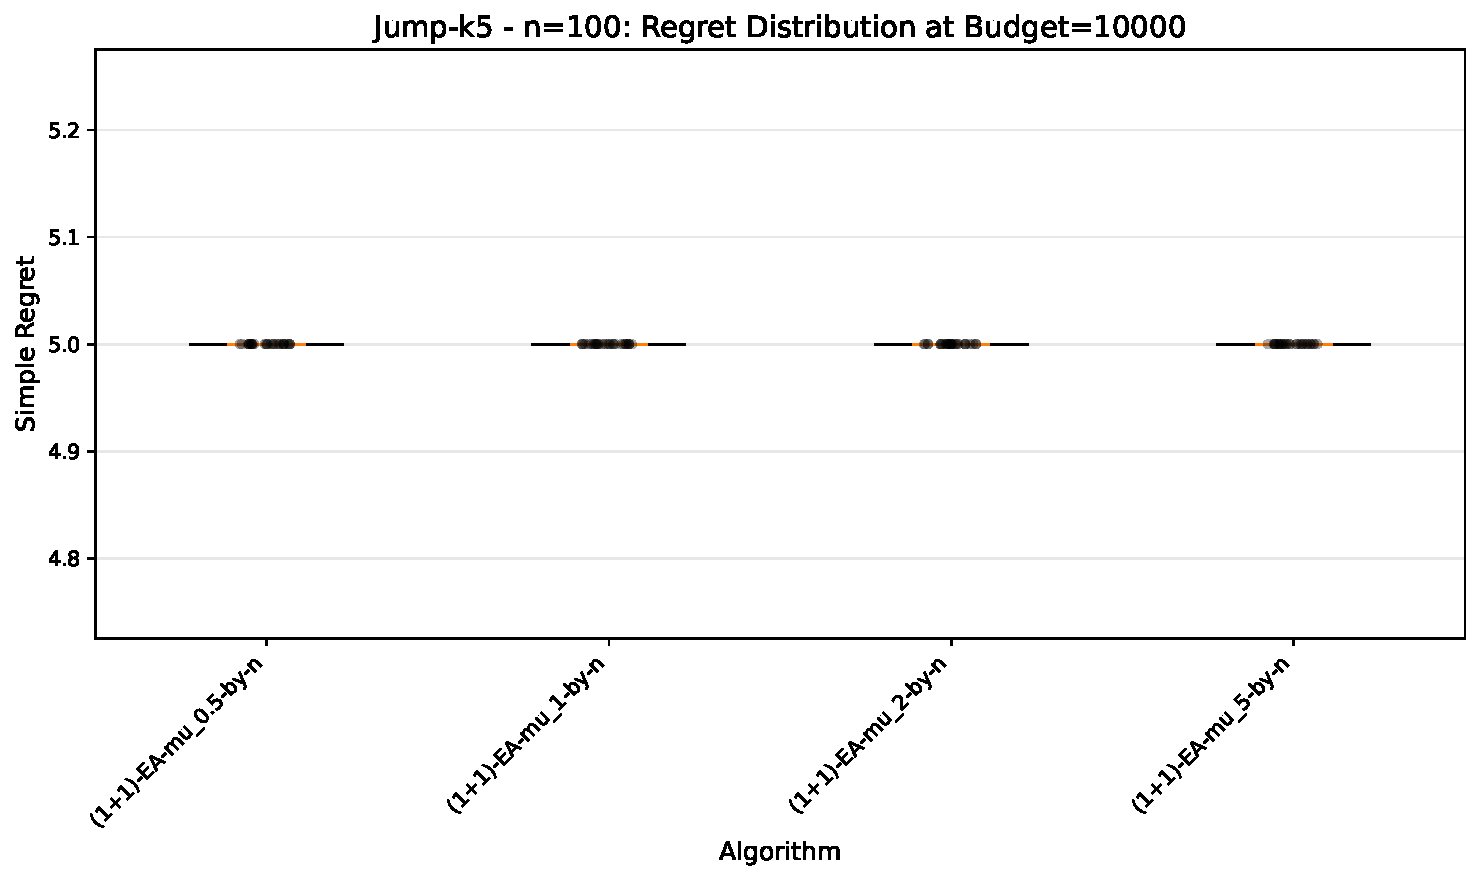
\includegraphics[width=0.80\textwidth]{results/barrier_mut/all_prob/jump_k5_regret_boxplot_b10000.pdf}
  \caption[Suite 10 representative regret distribution]{Suite~10
    budget-$10{,}000$ regret distribution for the representative
    \textsc{Jump}-$5$ archetype. The omitted convergence-probability panels for
    \textsc{Jump}-$5$, \textsc{Plateau}-$5$, and \textsc{Trap}-$5$ are exactly
    identical for the purpose used here: they show zero endpoint convergence for
    every mutation-rate variant, so the regret distribution is the more
    informative finite-budget diagnostic.}
  \label{fig:suite10-regret-boxplot}
\end{figure}

\begin{figure}[!htbp]
  \centering
  \begin{subfigure}[t]{0.48\textwidth}
    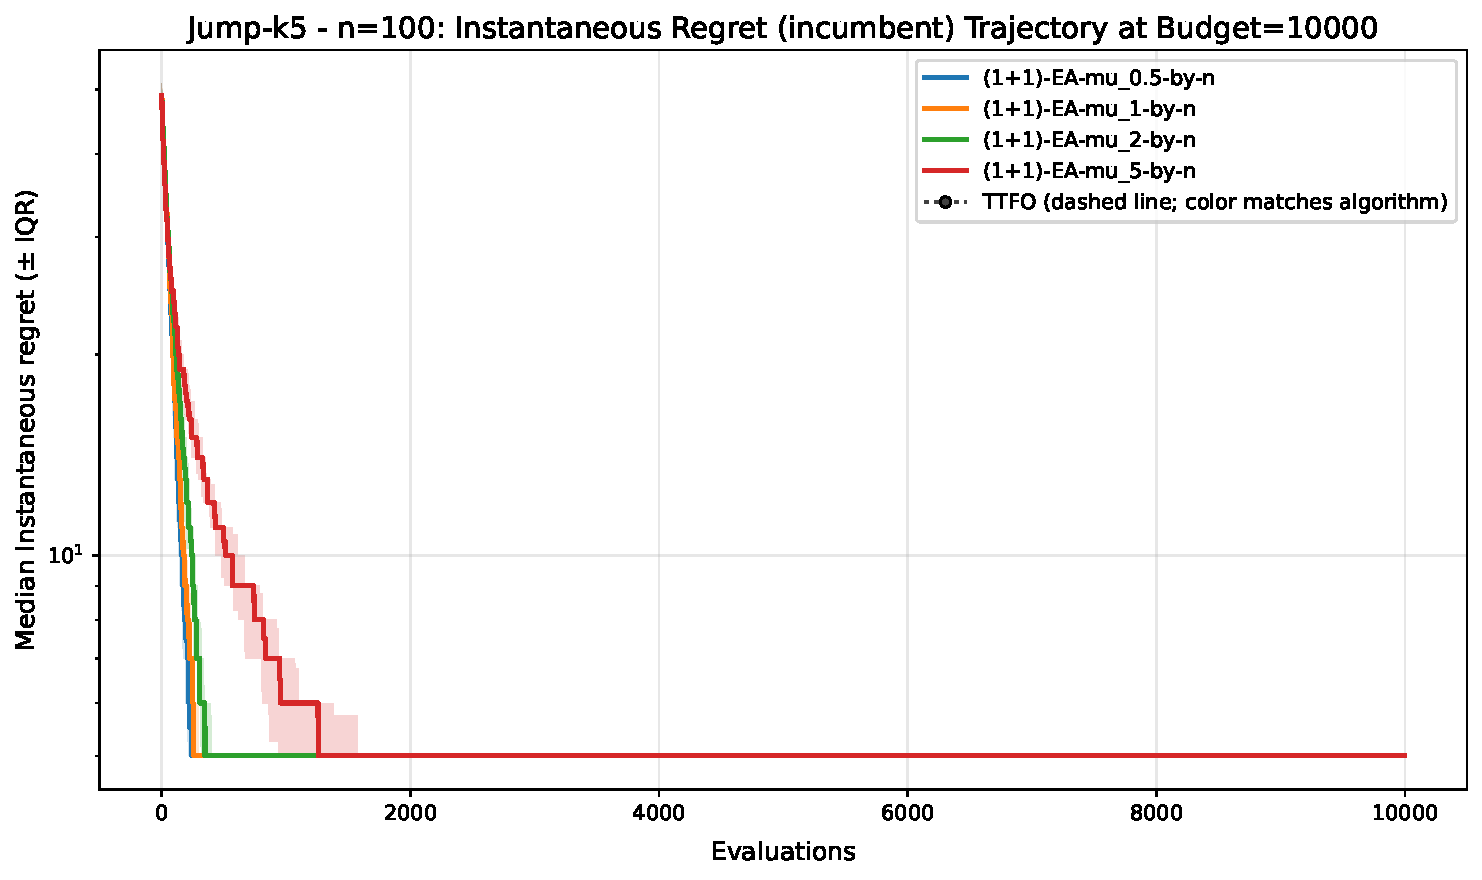
\includegraphics[width=\linewidth]{results/barrier_mut/all_prob/jump_k5_history_regret_instantaneous_best.pdf}
    \caption{\textsc{Jump}-$5$ instantaneous regret.}
    \label{fig:suite10-jump-k5-ir}
  \end{subfigure}
  \begin{subfigure}[t]{0.48\textwidth}
    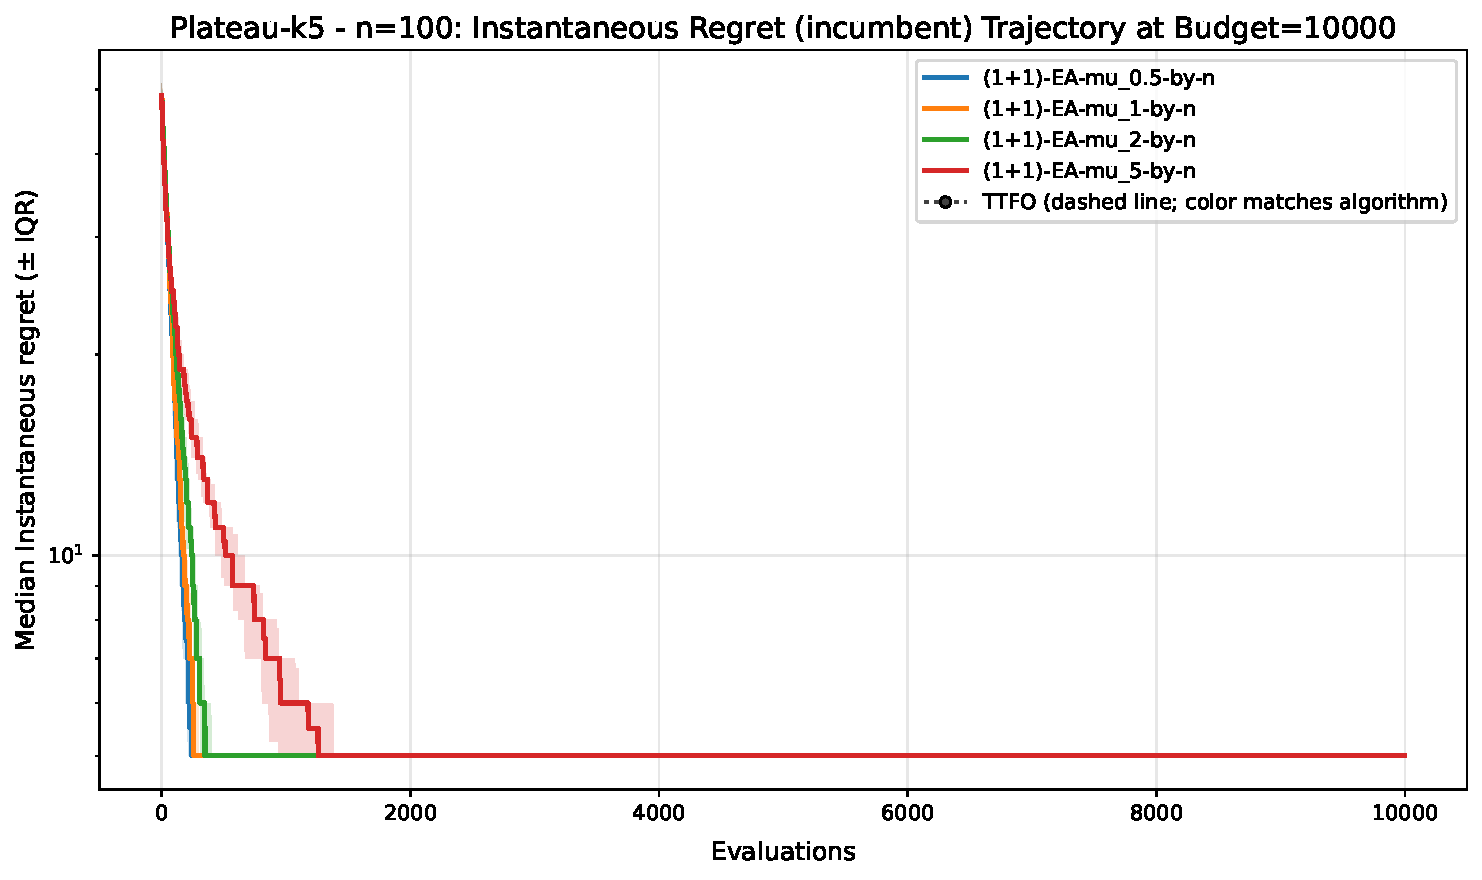
\includegraphics[width=\linewidth]{results/barrier_mut/all_prob/plateau_k5_history_regret_instantaneous_best.pdf}
    \caption{\textsc{Plateau}-$5$ instantaneous regret.}
    \label{fig:suite10-plateau-k5-ir}
  \end{subfigure}
  \begin{subfigure}[t]{0.80\textwidth}
    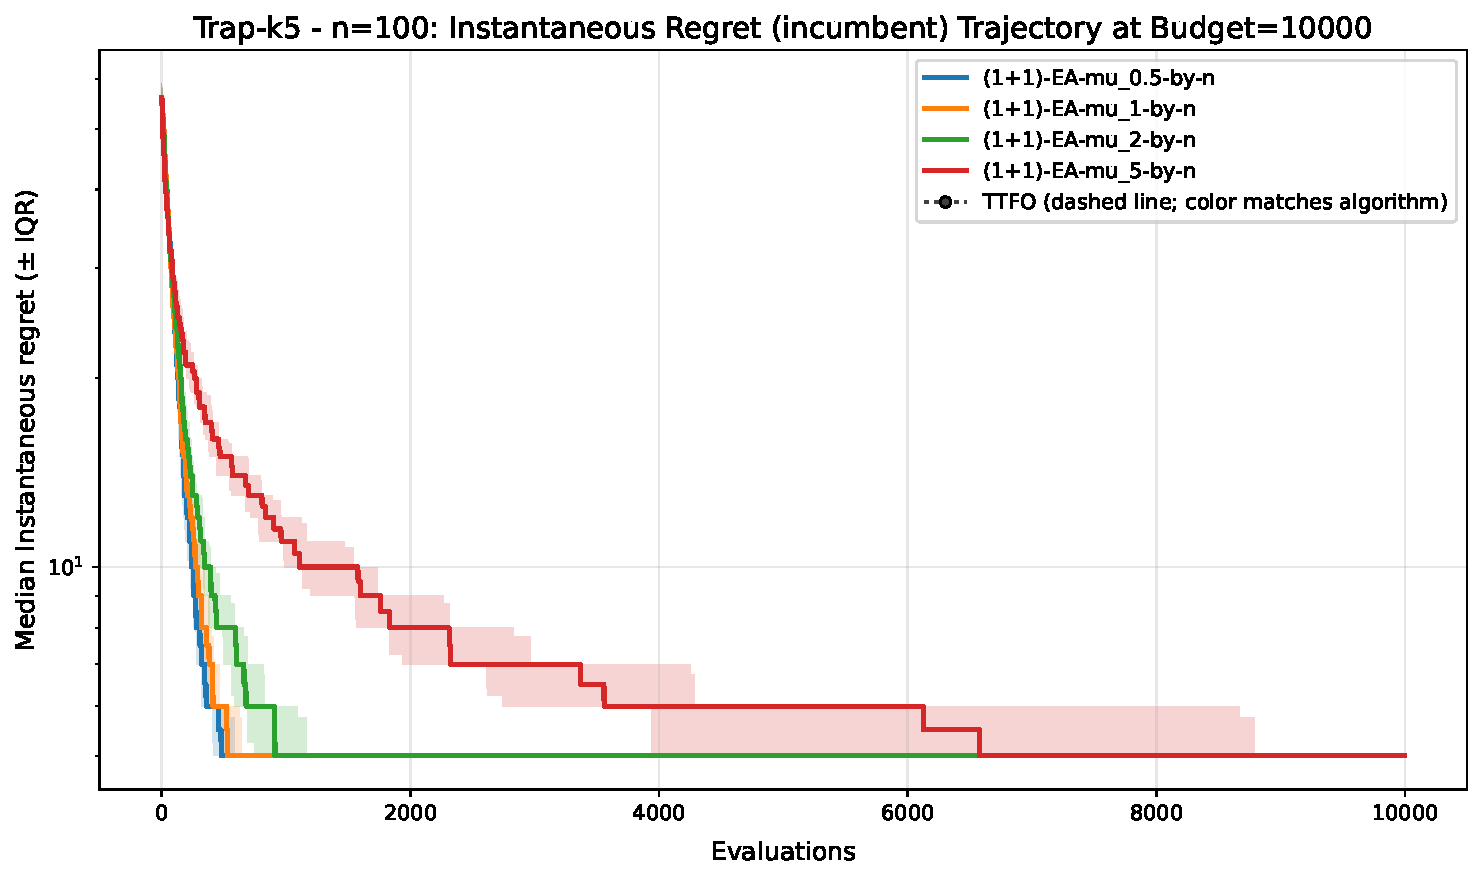
\includegraphics[width=\linewidth]{results/barrier_mut/all_prob/trap_k5_history_regret_instantaneous_best.pdf}
    \caption{\textsc{Trap}-$5$ instantaneous regret.}
    \label{fig:suite10-trap-k5-ir}
  \end{subfigure}
  \caption[Suite 10 barrier-archetype instantaneous regret]{Suite~10
    incumbent \acrshort{ir} trajectories for the three $k=5$ barrier
    archetypes. The plots expose the trapped-regret floors even when
    convergence probability is uniformly uninformative.}
  \label{fig:suite10-ir}
\end{figure}

\begin{figure}[!htbp]
  \centering
  \begin{subfigure}[t]{0.48\textwidth}
    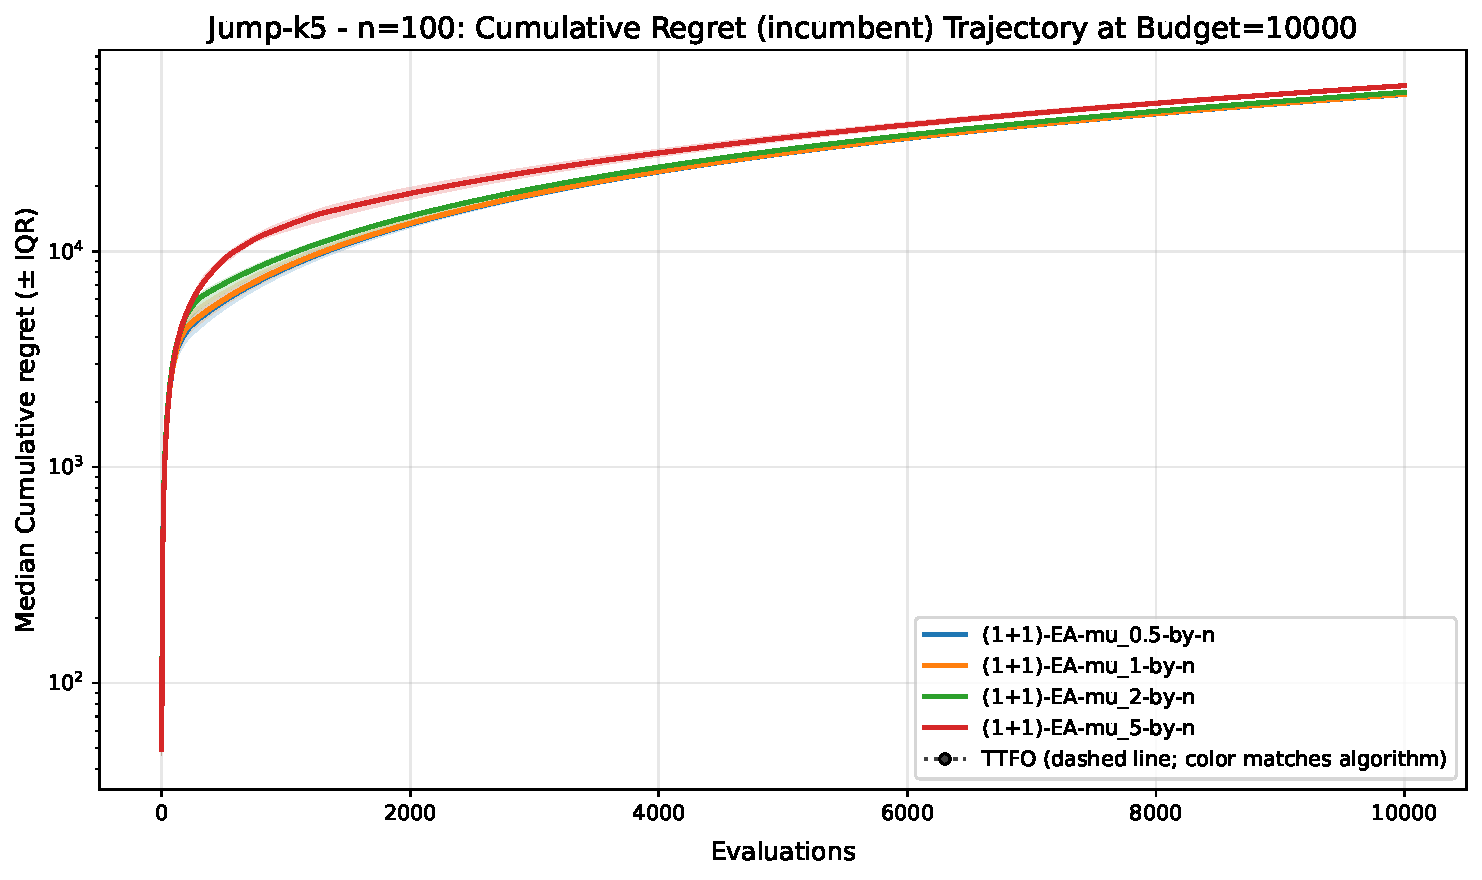
\includegraphics[width=\linewidth]{results/barrier_mut/all_prob/jump_k5_history_regret_cumulative_best.pdf}
    \caption{\textsc{Jump}-$5$ cumulative regret.}
    \label{fig:suite10-jump-k5-cr}
  \end{subfigure}
  \begin{subfigure}[t]{0.48\textwidth}
    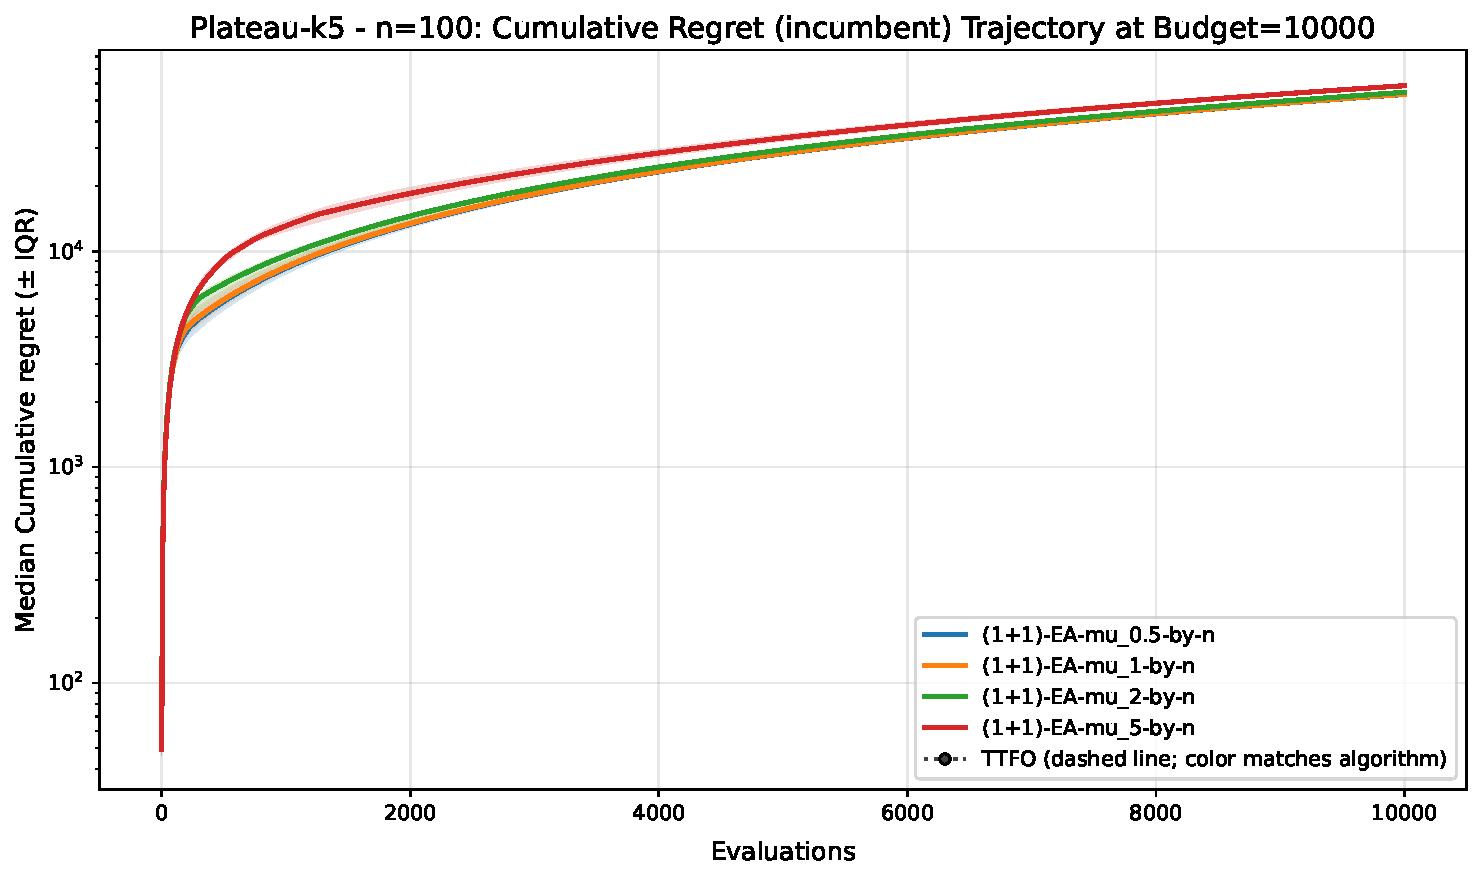
\includegraphics[width=\linewidth]{results/barrier_mut/all_prob/plateau_k5_history_regret_cumulative_best.pdf}
    \caption{\textsc{Plateau}-$5$ cumulative regret.}
    \label{fig:suite10-plateau-k5-cr}
  \end{subfigure}
  \begin{subfigure}[t]{0.80\textwidth}
    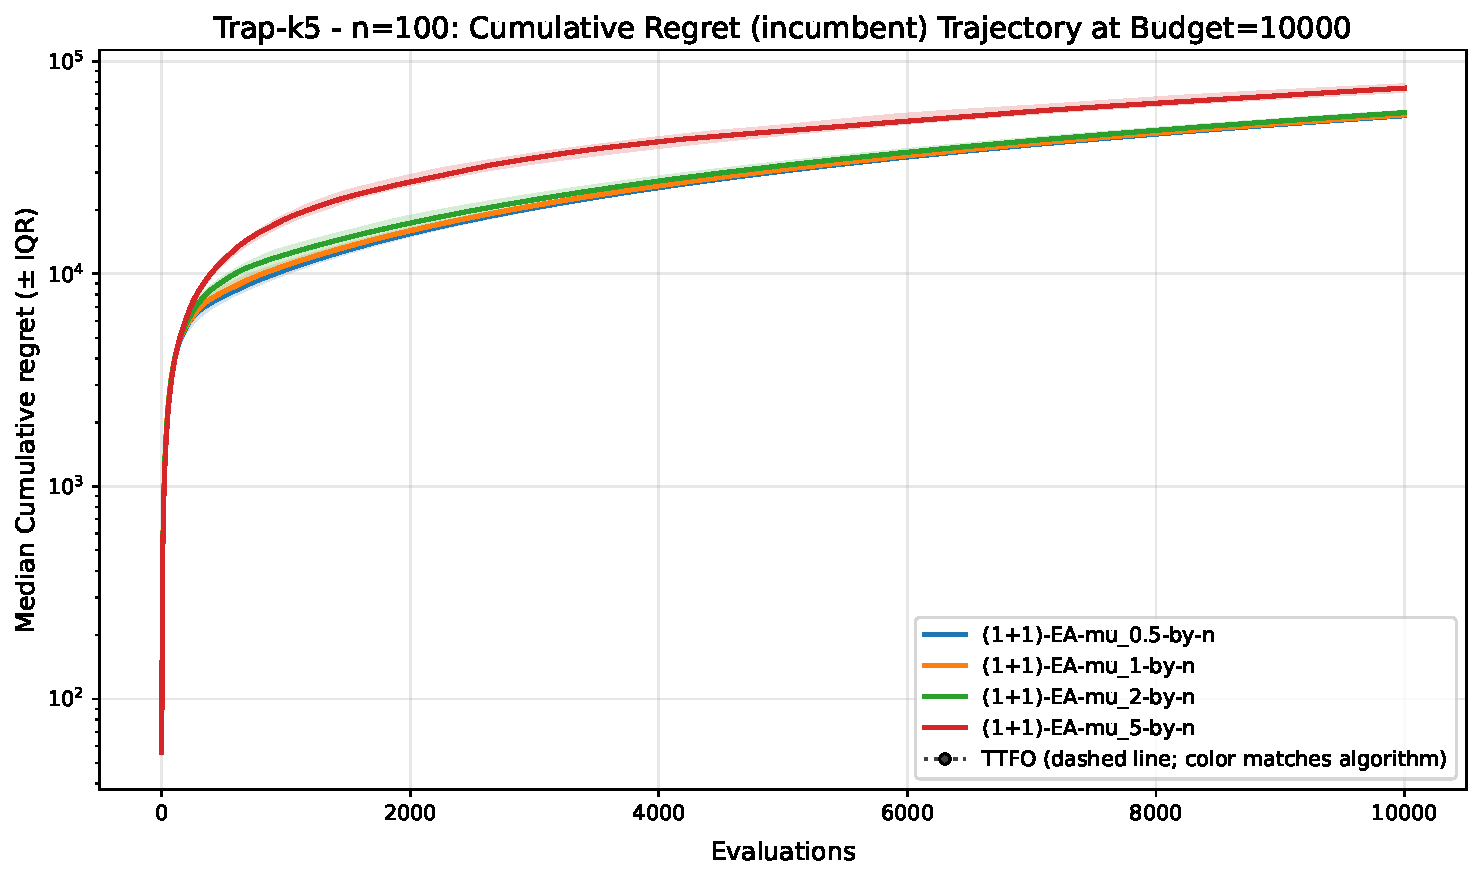
\includegraphics[width=\linewidth]{results/barrier_mut/all_prob/trap_k5_history_regret_cumulative_best.pdf}
    \caption{\textsc{Trap}-$5$ cumulative regret.}
    \label{fig:suite10-trap-k5-cr}
  \end{subfigure}
  \caption[Suite 10 barrier-archetype cumulative regret]{Suite~10
    incumbent \acrshort{cr} trajectories for the three $k=5$ barrier
    archetypes. The cumulative curves record the cost of each trapped phase
    under identical mutation-rate variants and budget.}
  \label{fig:suite10-cr}
\end{figure}

The \textsc{Jump}-$5$ and \textsc{Plateau}-$5$ incumbent
\acrshort{cr} curves remain close in shape, matching the behavior
already observed in the Suite~06 matched comparison~\ref{fig:suite06-plateau-jump-k2}. At this
width, the neutral-walk and gap-crossing mechanisms induce similar
realized \acrshort{ir} curves under the tested mutation rates, so their cumulative
curves primarily record comparable optimization cost rather than a
visibly separate barrier signature (Figures~\ref{fig:suite10-ir}
and~\ref{fig:suite10-cr}).

The \textsc{Trap}-$5$ median incumbent \acrshort{ir} trajectories
show a clearer contrast. Across all four mutation-rate variants, the
algorithm spends substantially longer at intermediate fitness
levels before settling into the deceptive basin with residual regret
approximately $k$ (Figure~\ref{fig:suite10-trap-k5-ir}). This extended intermediate phase is
consistent with the deceptive gradient: progress can continue locally,
but it carries the search toward the wrong basin rather than toward the
global optimum.

Thus, although no method solves any of the three instances within the
budget, the trajectory plots still expose how each barrier shapes the
cost of failure.

\section{NK Ruggedness and SA Cooling}
\label{sec:results:nk}

\subsection{Suite 11: SA Cooling Schedule Diagnostics}
\label{sec:results:suite11}
\begin{figure}[!htbp]
  \centering
  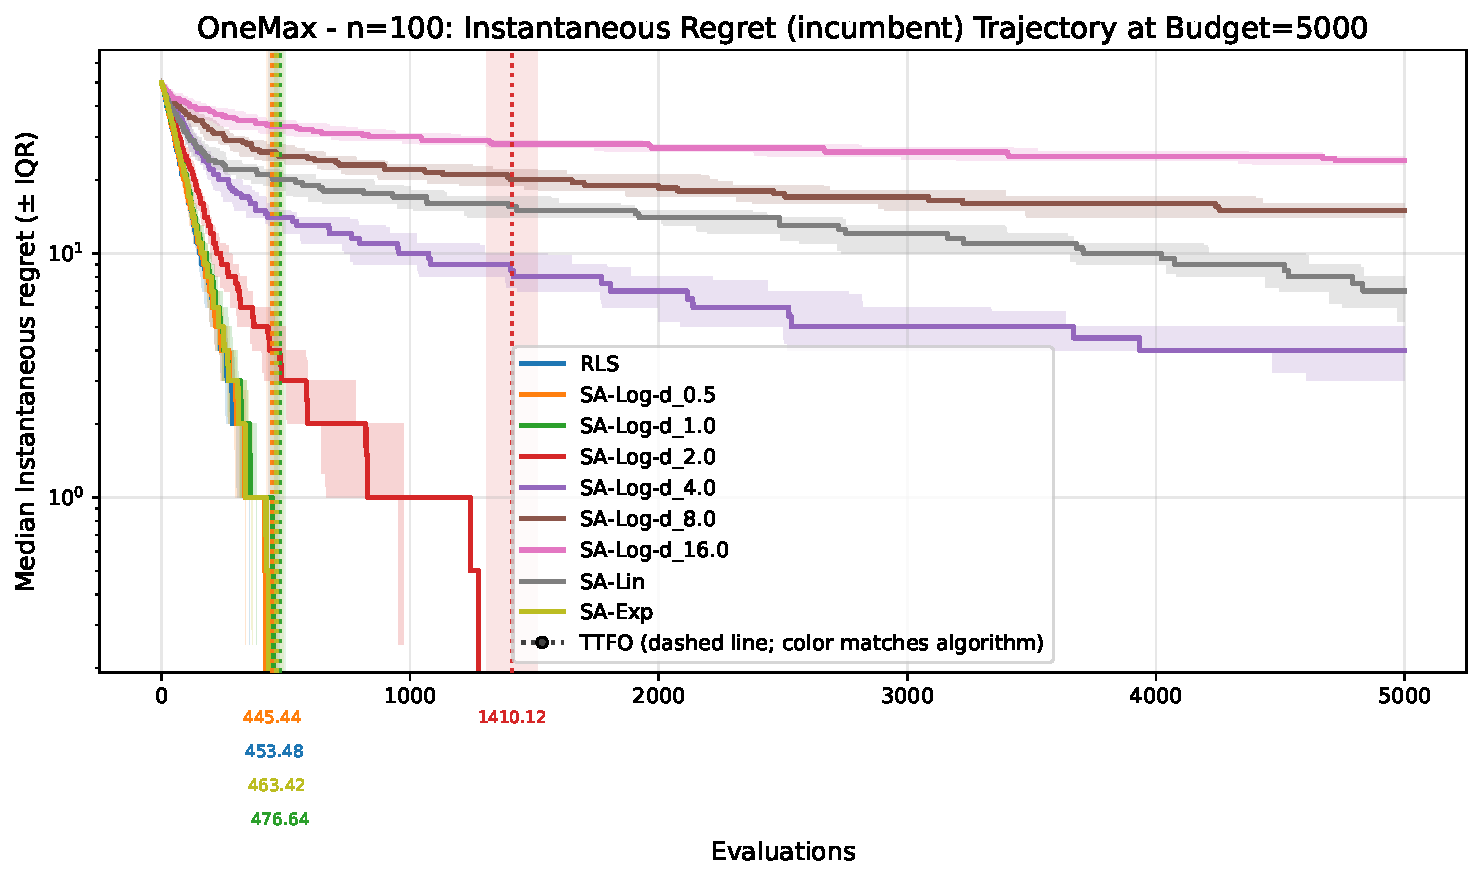
\includegraphics[width=0.80\textwidth]{results/nk_sa/sa_cooling_onemax_history_regret_instantaneous.pdf}
  \caption[Suite 11 SA cooling trajectories]{Suite~11 incumbent
    \acrshort{ir} trajectories on
    \textsc{OneMax} for \acrshort{rls} and simulated-annealing cooling
    schedules. The onset of each low-regret floor gives a direct visual
  diagnostic of effective cooling speed.}
  \label{fig:suite11-sa-cooling-ir}
\end{figure}

The instantaneous regret trajectories show a clear ordering in the
effective cooling, or for RLS, stabilization, time of the methods.
The empirical ordering is
\begin{multline*}
  \text{RLS} \;<\; \text{SA-Exp} \;<\; \text{SA-Log}_{d=0.5} \;<\;
  \text{SA-Log}_{d=1} \\ \;<\; \text{SA-Log}_{d=2} \;<\;
  \text{SA-Log}_{d=4} \;<\; \text{SA-Lin} \;<\; \text{SA-Log}_{d=8}
  \;<\; \text{SA-Log}_{d=16},
\end{multline*}
where earlier position denotes earlier convergence to a low-regret
plateau. Thus, the log-scale \acrshort{ir} curves provide a direct
diagnostic of schedule aggressiveness: fast schedules collapse
quickly, while slower logarithmic schedules preserve exploration
longer and delay stabilization. This supports the suite hypothesis
that cooling schedules leave visible trajectory-level signatures,
rather than only changing final regret values; see
Figure~\ref{fig:suite11-sa-cooling-ir}.

\subsection{Suite 03: NK Ruggedness --- Cooling $\times$ Epistasis Grid}
\label{sec:results:suite03}

\begin{figure}[!htbp]
  \centering
  \begin{subfigure}[t]{0.48\textwidth}
    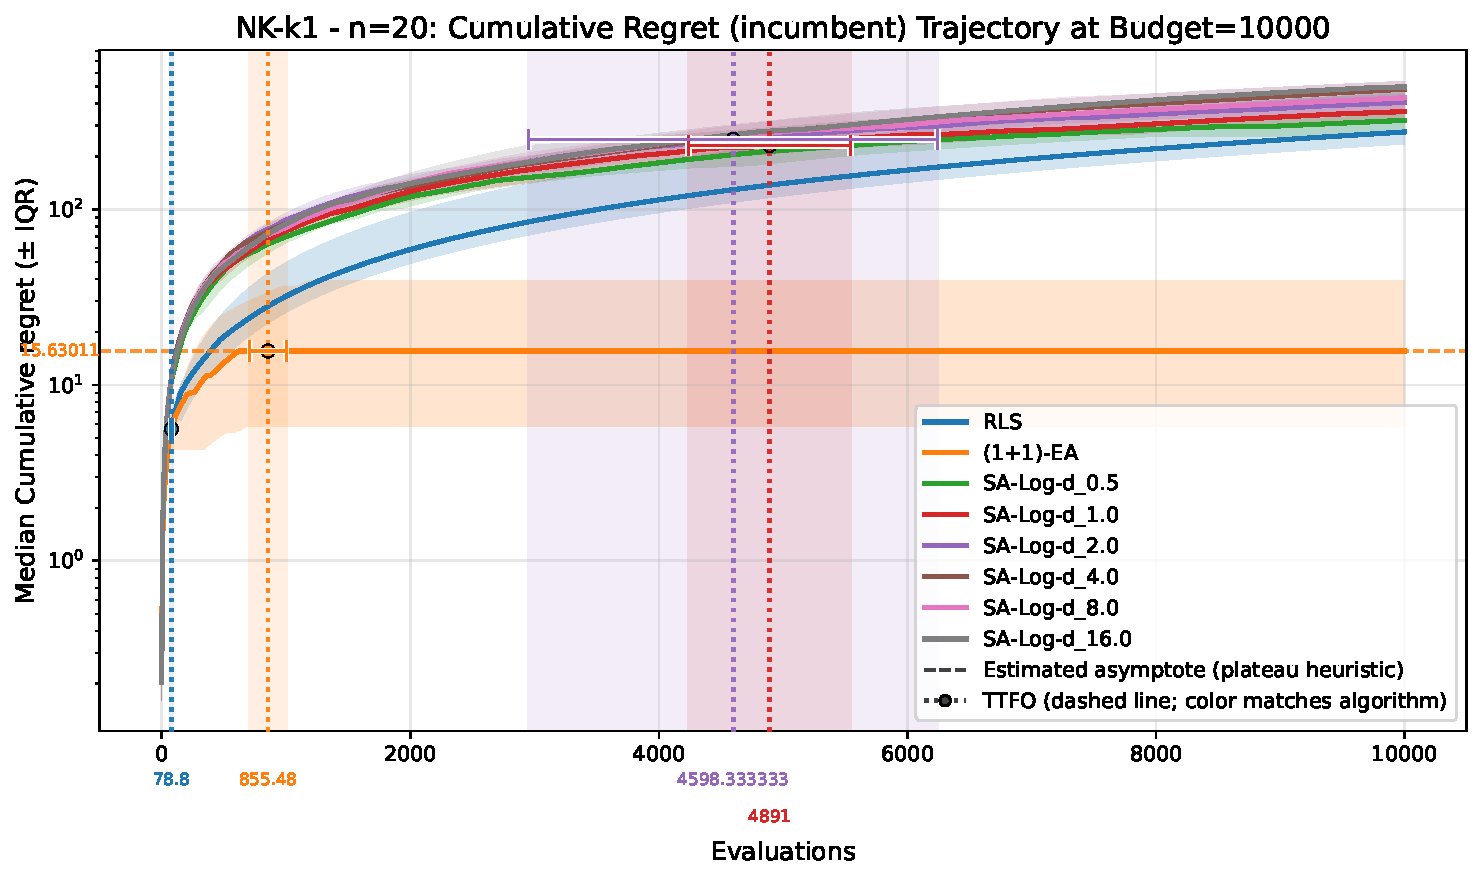
\includegraphics[width=\linewidth]{results/nk_sa/suite03_k1_history_regret_cumulative_best.pdf}
    \caption{NK landscape with $k=1$.}
    \label{fig:suite03-k1-cr}
  \end{subfigure}
  \begin{subfigure}[t]{0.48\textwidth}
    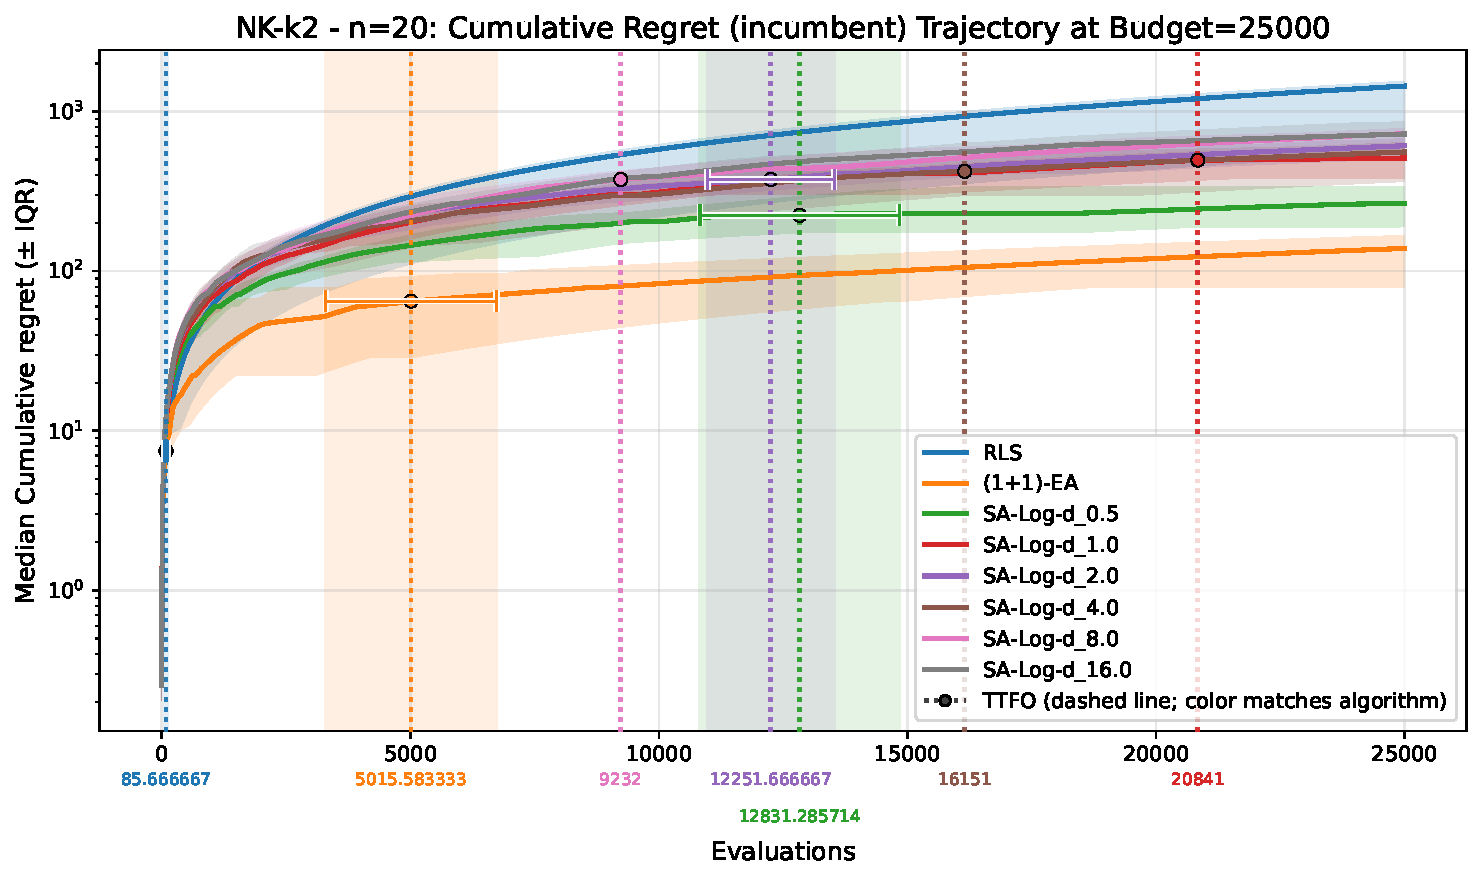
\includegraphics[width=\linewidth]{results/nk_sa/suite03_k2_history_regret_cumulative_best.pdf}
    \caption{NK landscape with $k=2$.}
    \label{fig:suite03-k2-cr}
  \end{subfigure}
  \begin{subfigure}[t]{0.80\textwidth}
    \includegraphics[width=\linewidth]{results/nk_sa/suite03_k4_history_regret_cumulative_best.pdf}
    \caption{NK landscape with $k=4$.}
    \label{fig:suite03-k4-cr}
  \end{subfigure}
  \caption[Suite 03 NK \acrshort{cr} trajectories]{Suite~03
    incumbent \acrshort{cr} trajectories across
    increasing NK epistasis. Low-epistasis instances favour mutation-only
    baselines, while at $k=4$ the slower logarithmic cooling schedule begins to
  dominate after a longer transient phase.}
  \label{fig:suite03-cr}
\end{figure}

\begin{figure}[!htbp]
  \centering
  \begin{subfigure}[t]{0.48\textwidth}
    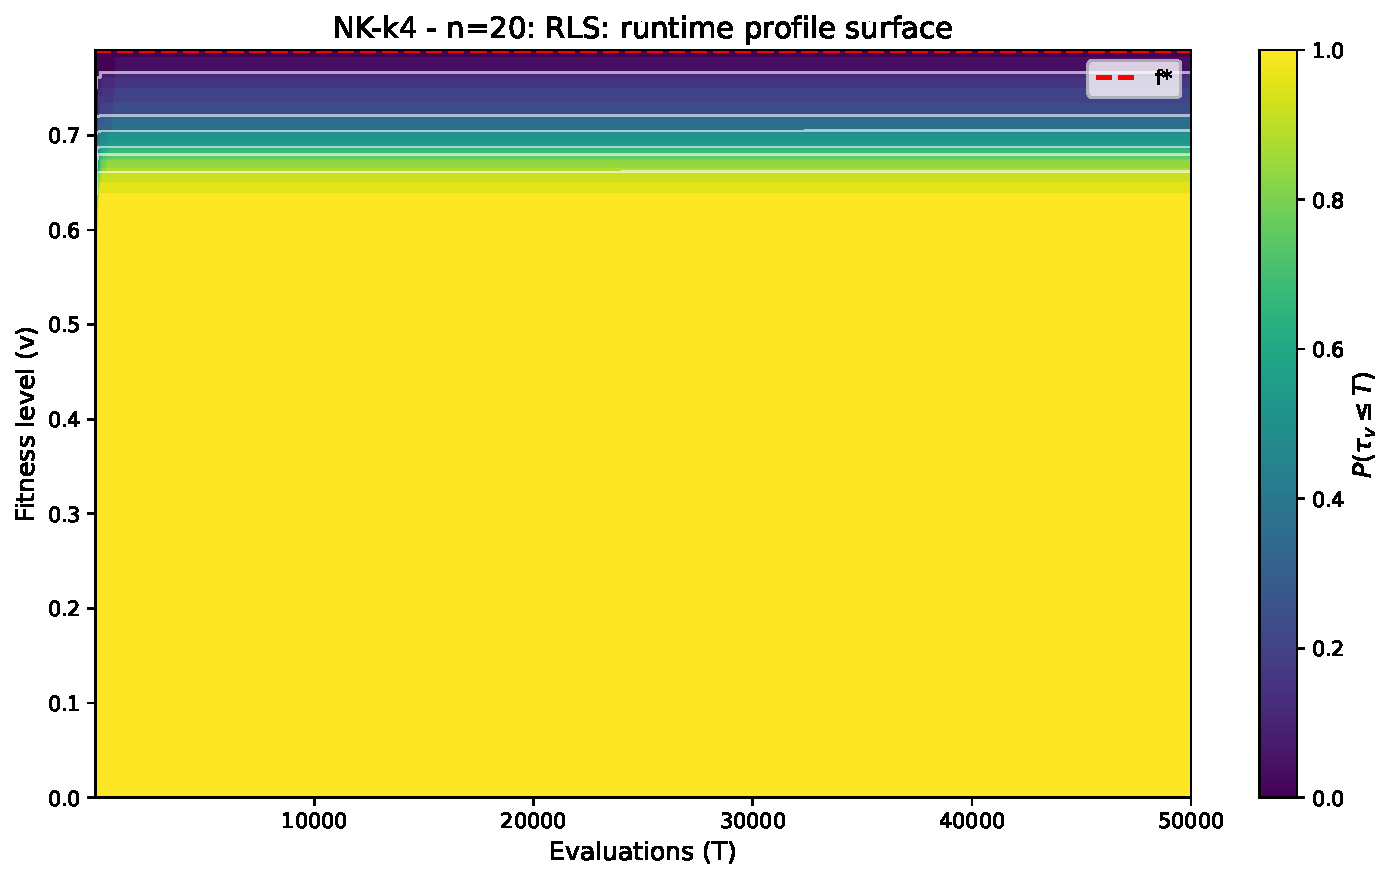
\includegraphics[width=\linewidth]{results/nk_sa/suite03_k4_inverse_runtime_profile_surface_RLS.pdf}
    \caption{\acrshort{rls} on NK $k=4$.}
    \label{fig:suite03-k4-profile-rls}
  \end{subfigure}
  \begin{subfigure}[t]{0.48\textwidth}
    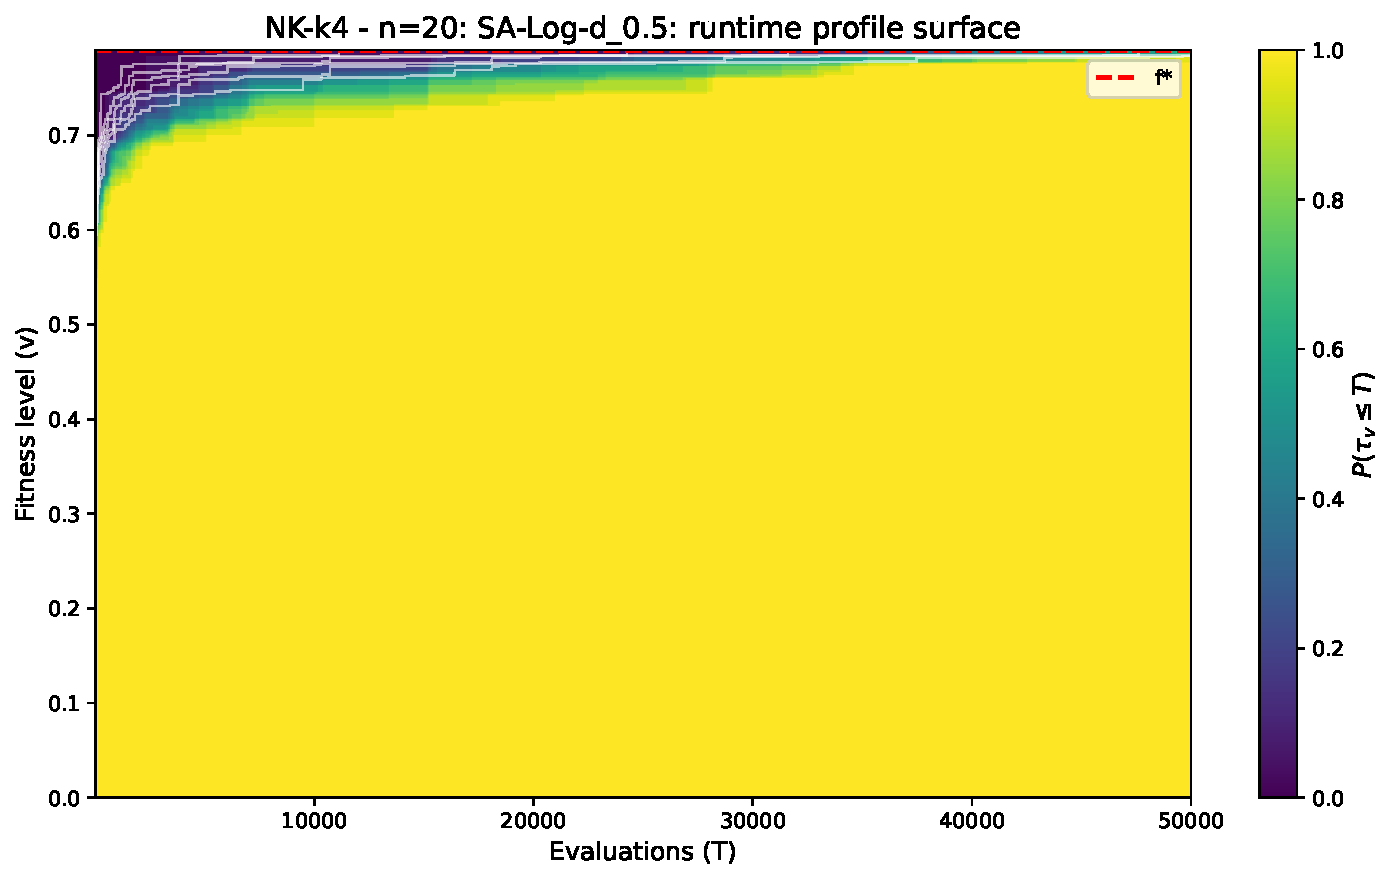
\includegraphics[width=\linewidth]{results/nk_sa/suite03_k4_inverse_runtime_profile_surface_SA-Log-d_0.5.pdf}
    \caption{\acrshort{sa}-Log with $d=0.5$ on NK $k=4$.}
    \label{fig:suite03-k4-profile-sa-log-d05}
  \end{subfigure}
  \caption[Suite 03 NK inverse runtime profiles]{Representative
    Suite~03 inverse runtime profile surfaces for NK
    $k=4$. The saturation frontiers show where each algorithm ceases to make
  reliable progress toward higher fitness levels.}
  \label{fig:suite03-profiles}
\end{figure}

Suite~03 shows a clear regime split between low and moderate
epistasis. For $k=1$ and $k=2$, all \acrshort{sa} variants underperform the
baselines in incumbent cumulative regret, indicating that
cooling-induced exploration is not compensated by ruggedness at these
settings (Figure~\ref{fig:suite03-k2-cr}). The effect is strongest at
$k=1$, where the $(1+1)$-\acrshort{ea} is
the only method whose median incumbent \acrshort{cr} curve
reaches a horizontal asymptote at the optimum, stabilizing at
approximately $15.63$ cumulative regret (Figure~\ref{fig:suite03-k1-cr}).
This ordering reverses for $k \ge 4$: \acrshort{sa} with
logarithmic cooling at $d=0.5$ accumulates the least regret overall
and separates clearly from RLS and the $(1+1)$-\acrshort{ea}, although no median
curve converges within the evaluation budget, as expected on these
rugged instances. At $k=4$, the \acrshort{sa}-\acrshort{log}-$d=0.5$
curve crosses below
the $(1+1)$-\acrshort{ea} at roughly $3.3\times 10^4$ evaluations, marking the
budget at which slower exploratory progress begins to dominate greedy
improvement (Figure~\ref{fig:suite03-k4-cr}). The inverse runtime profile
surfaces corroborate
this interpretation: across the grid, \acrshort{rls} exhibits a truncated
frontier consistent with entrapment in a local optimum, visible from
the contour boundary of the corresponding surface
(Figure~\ref{fig:suite03-profiles}).
% ~200 words
%
\subsection{Suite 12: NK Saturation}
\label{sec:results:suite12}
\begin{figure}[!htbp]
  \centering
  \begin{subfigure}[t]{0.48\textwidth}
    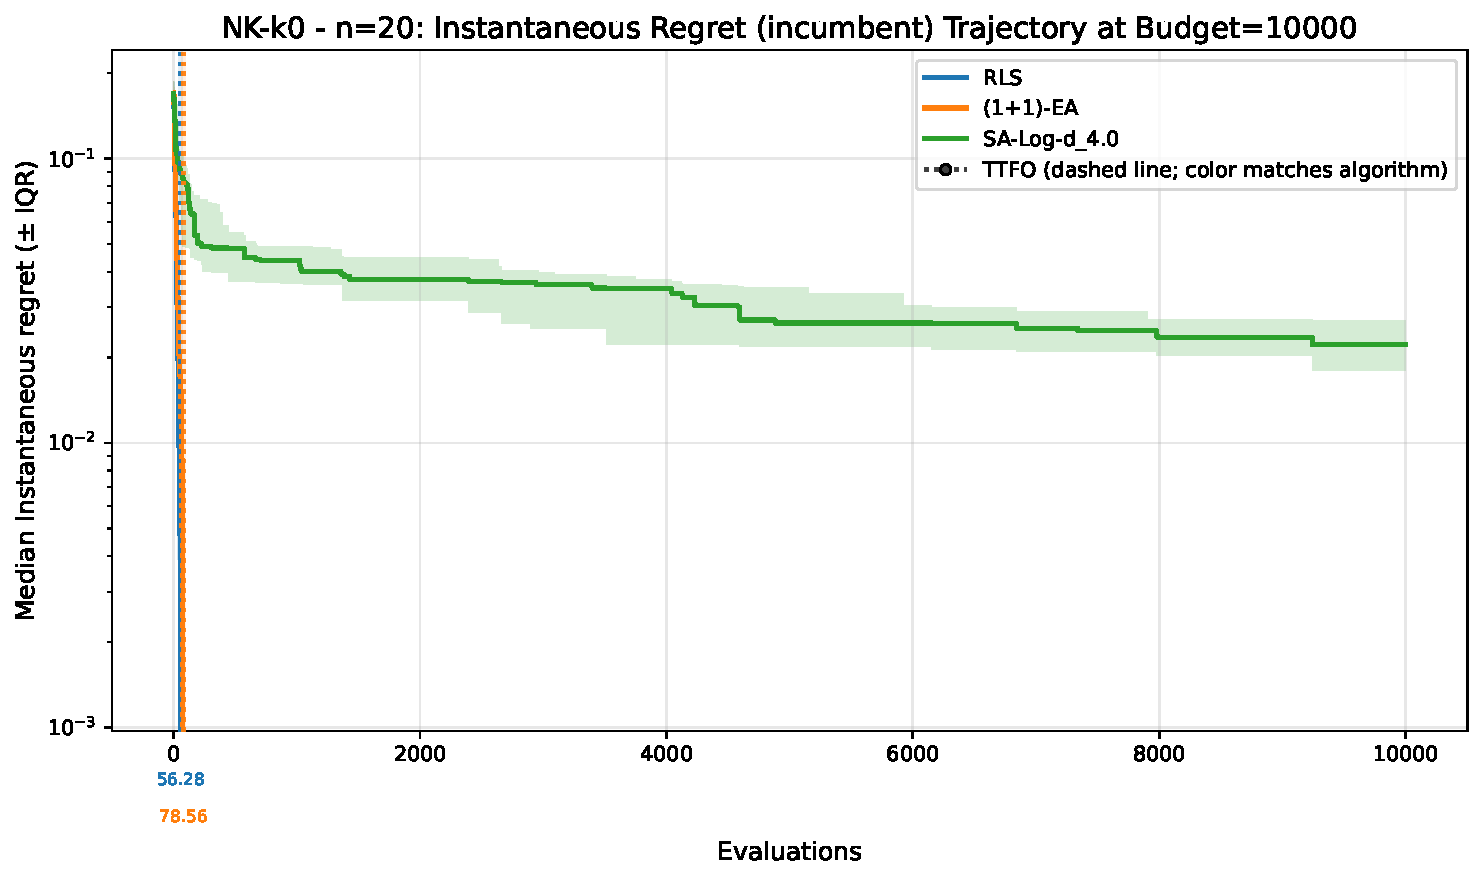
\includegraphics[width=\linewidth]{results/nk_sa/suite12_k0_history_regret_instantaneous_best.pdf}
    \caption{NK $k=0$.}
    \label{fig:suite12-ir-k0}
  \end{subfigure}
  \begin{subfigure}[t]{0.48\textwidth}
    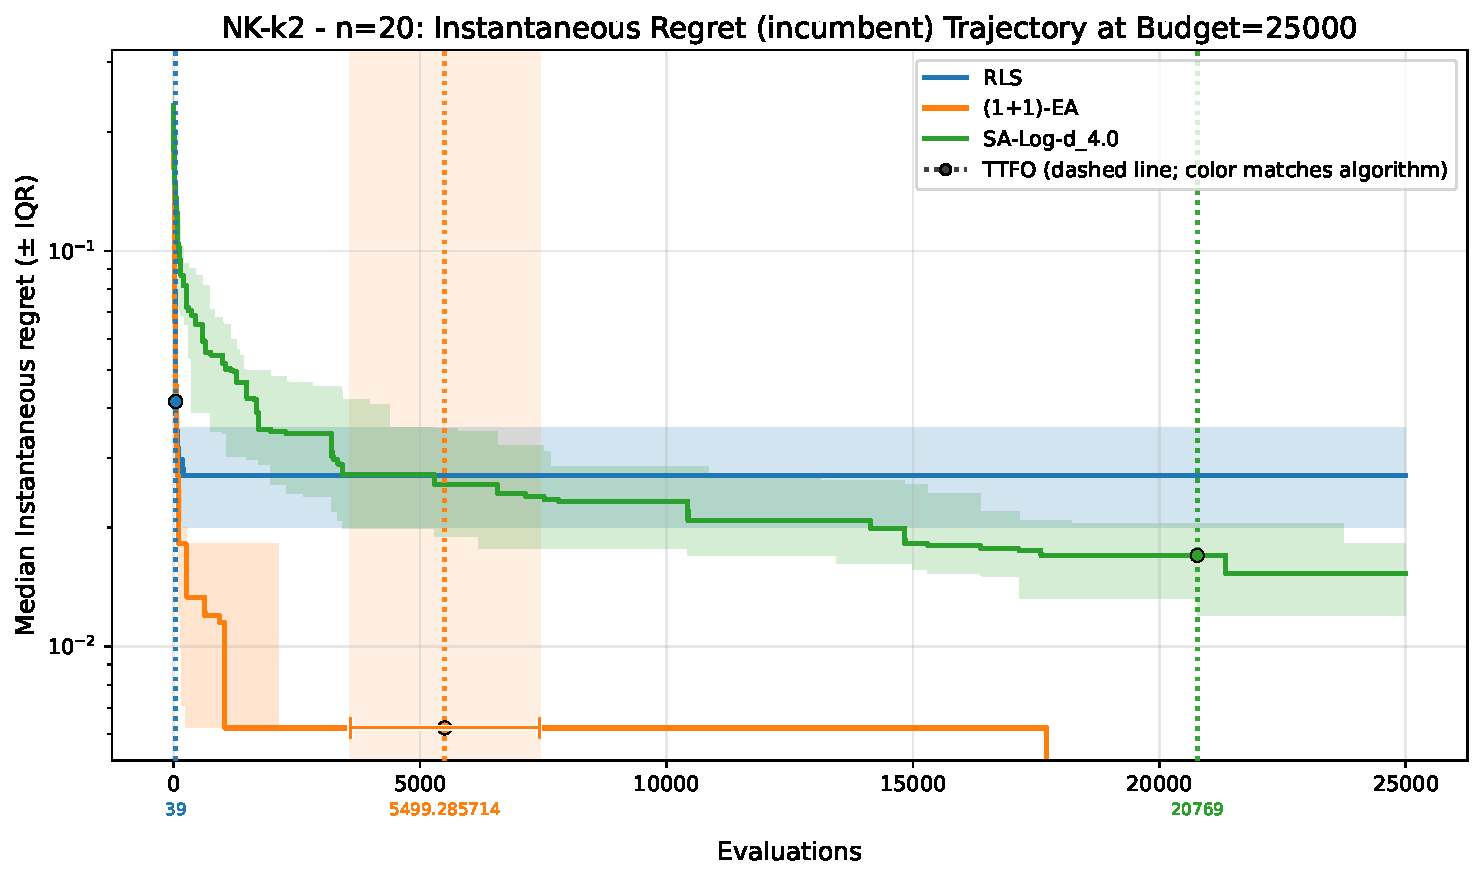
\includegraphics[width=\linewidth]{results/nk_sa/suite12_k2_history_regret_instantaneous_best.pdf}
    \caption{NK $k=2$.}
    \label{fig:suite12-ir-k2}
  \end{subfigure}
  \begin{subfigure}[t]{0.48\textwidth}
    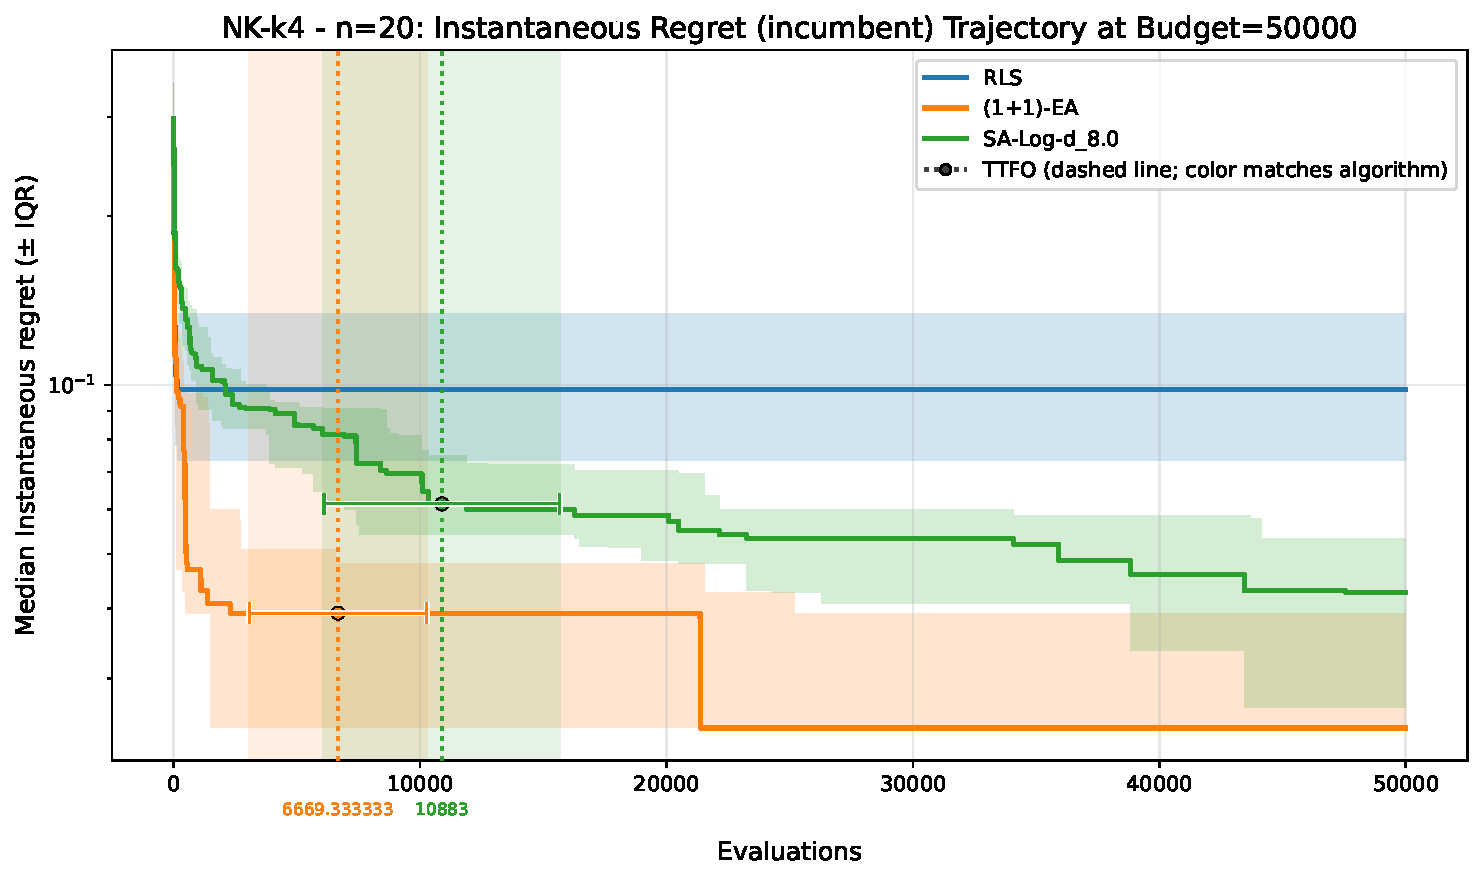
\includegraphics[width=\linewidth]{results/nk_sa/suite12_k4_history_regret_instantaneous_best.pdf}
    \caption{NK $k=4$.}
    \label{fig:suite12-ir-k4}
  \end{subfigure}
  \begin{subfigure}[t]{0.48\textwidth}
    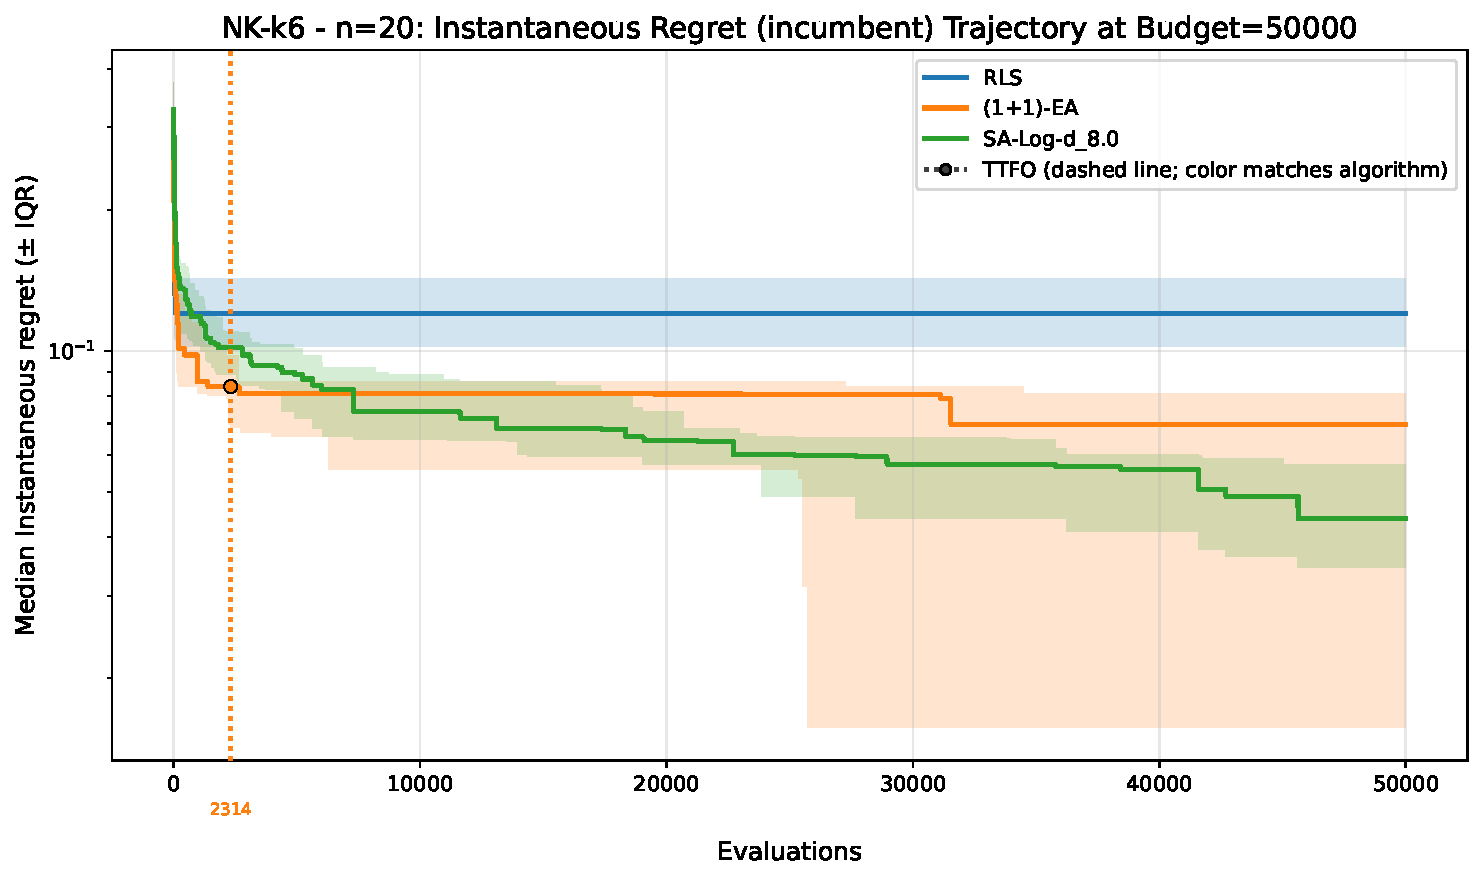
\includegraphics[width=\linewidth]{results/nk_sa/suite12_k6_history_regret_instantaneous_best.pdf}
    \caption{NK $k=6$.}
    \label{fig:suite12-ir-k6}
  \end{subfigure}
  \begin{subfigure}[t]{0.80\textwidth}
    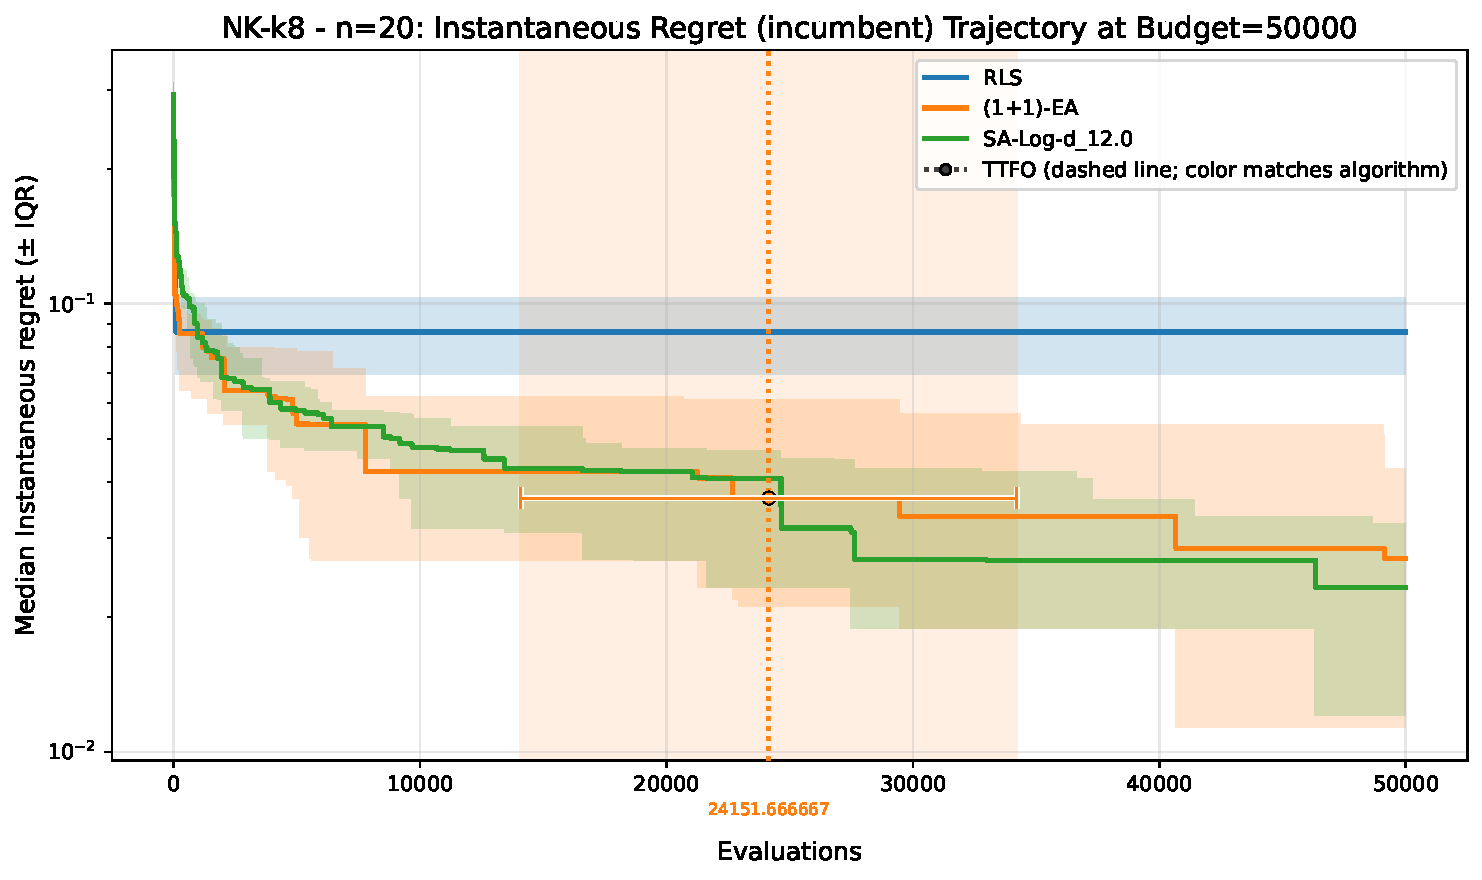
\includegraphics[width=\linewidth]{results/nk_sa/suite12_k8_history_regret_instantaneous_best.pdf}
    \caption{NK $k=8$.}
    \label{fig:suite12-ir-k8}
  \end{subfigure}
  \caption[Suite 12 calibrated-cooling regret trajectories]{Suite~12
    incumbent \acrshort{ir} trajectories under
    per-$k$ calibrated cooling. The terminal regret floor rises with epistasis,
    and calibrated simulated annealing becomes most useful on the more rugged
  $k=6$ and $k=8$ landscapes.}
  \label{fig:suite12-ir}
\end{figure}

\begin{figure}[!htbp]
  \centering
  \begin{subfigure}[t]{0.48\textwidth}
    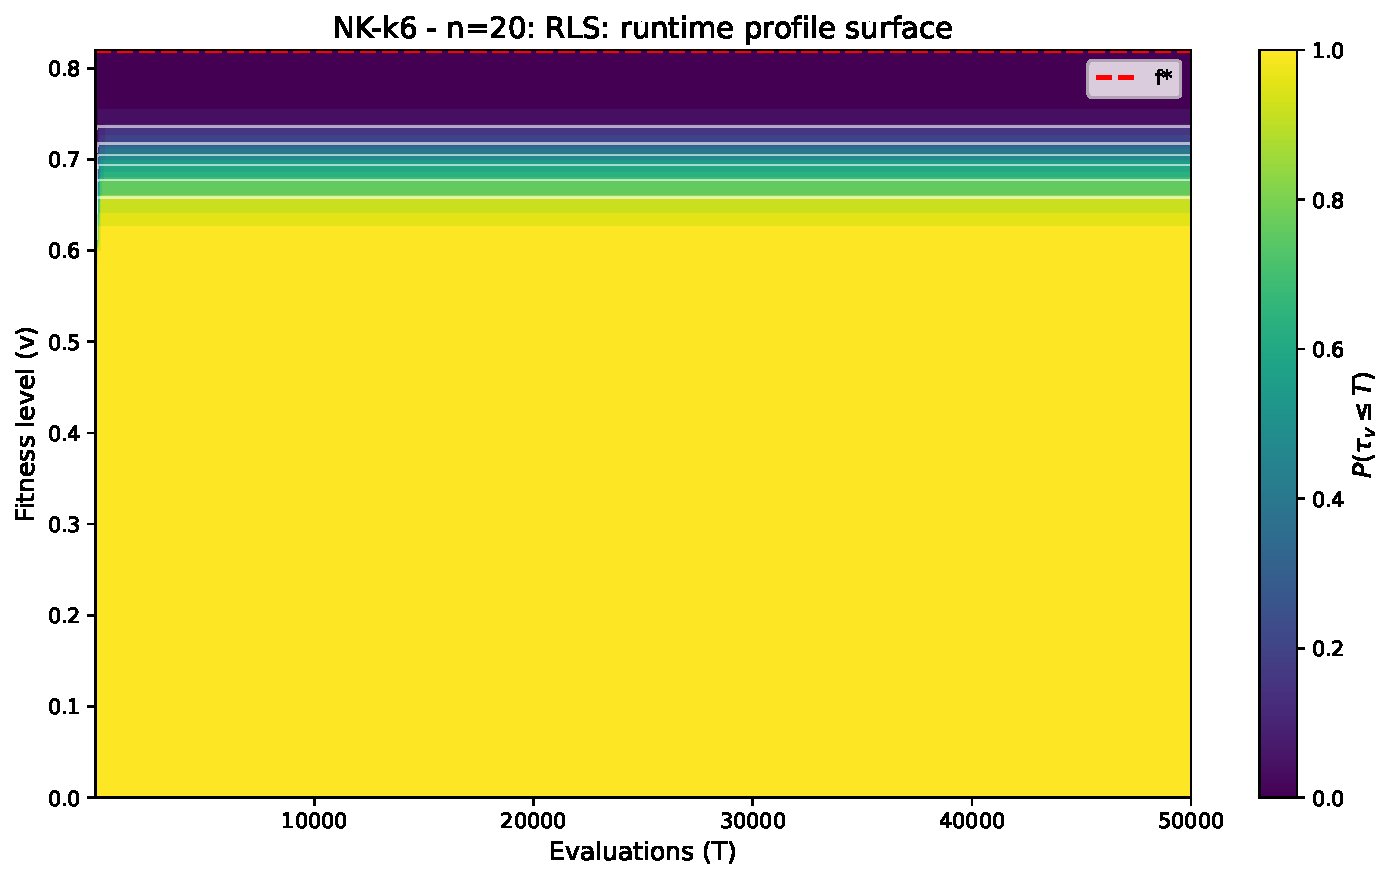
\includegraphics[width=\linewidth]{results/nk_sa/suite12_k6_inverse_runtime_profile_surface_RLS.pdf}
    \caption{\acrshort{rls} on NK $k=6$.}
    \label{fig:suite12-k6-profile-rls}
  \end{subfigure}
  \begin{subfigure}[t]{0.48\textwidth}
    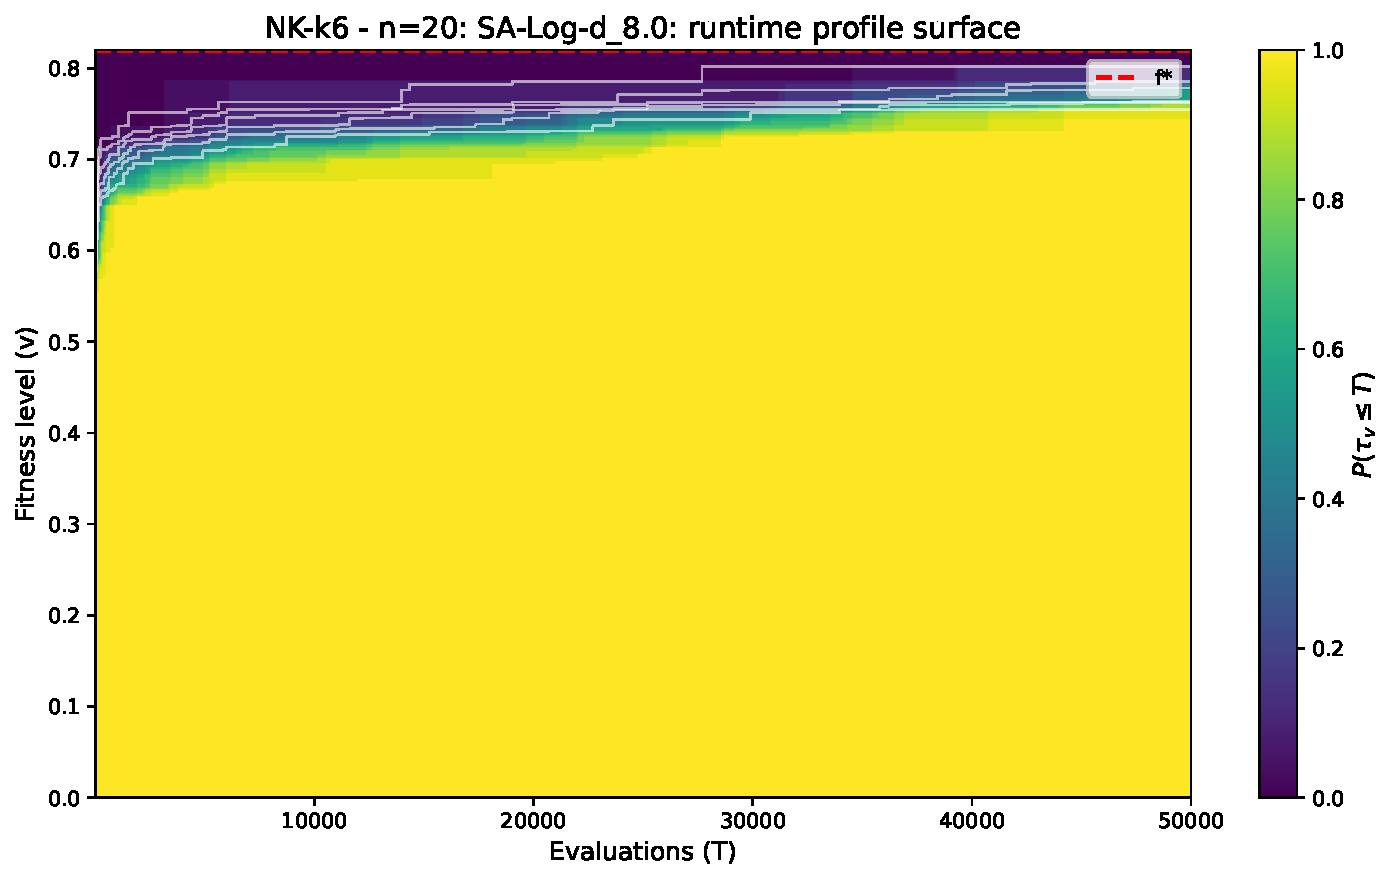
\includegraphics[width=\linewidth]{results/nk_sa/suite12_k6_inverse_runtime_profile_surface_SA-Log-d_8.0.pdf}
    \caption{Calibrated \acrshort{sa} on NK $k=6$.}
    \label{fig:suite12-k6-profile-sa}
  \end{subfigure}
  \begin{subfigure}[t]{0.48\textwidth}
    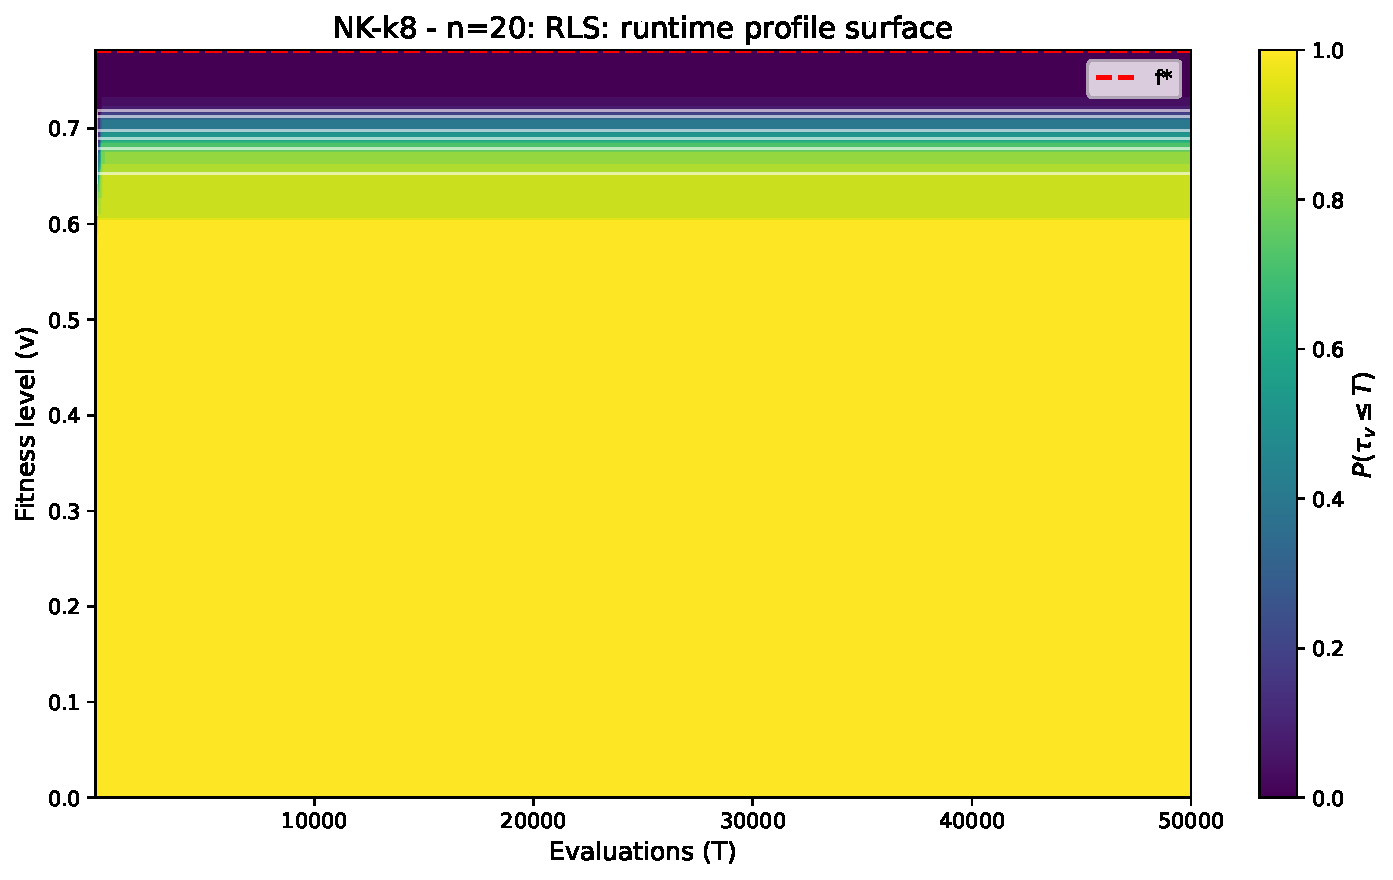
\includegraphics[width=\linewidth]{results/nk_sa/suite12_k8_inverse_runtime_profile_surface_RLS.pdf}
    \caption{\acrshort{rls} on NK $k=8$.}
    \label{fig:suite12-k8-profile-rls}
  \end{subfigure}
  \begin{subfigure}[t]{0.48\textwidth}
    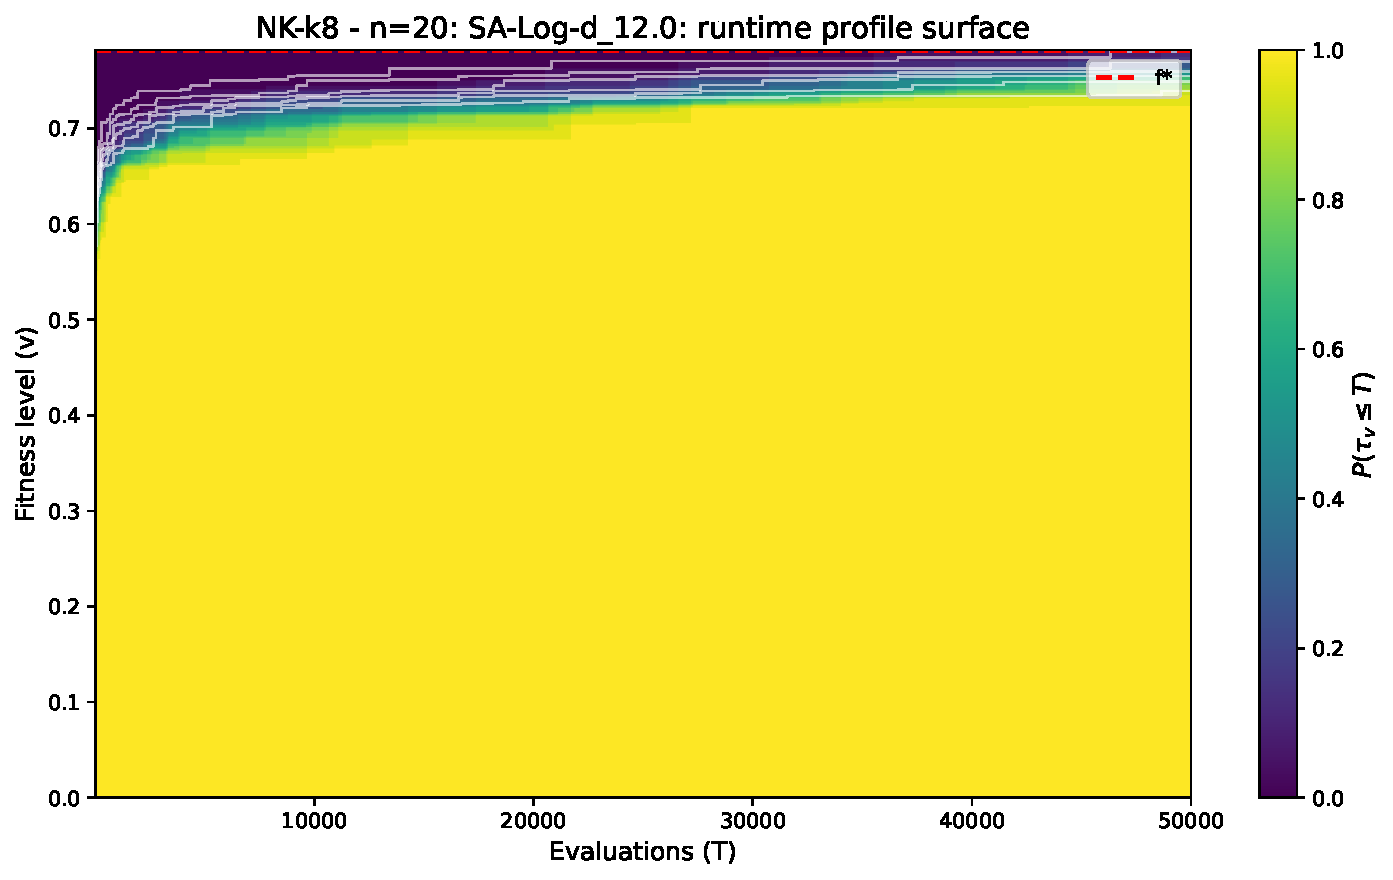
\includegraphics[width=\linewidth]{results/nk_sa/suite12_k8_inverse_runtime_profile_surface_SA-Log-d_12.0.pdf}
    \caption{Calibrated \acrshort{sa} on NK $k=8$.}
    \label{fig:suite12-k8-profile-sa}
  \end{subfigure}
  \caption[Suite 12 high-epistasis NK profiles]{Suite~12 inverse
    runtime profile surfaces for higher-epistasis NK
    landscapes. The RLS surfaces saturate below the optimum, while calibrated
    simulated annealing maintains progress to higher fitness levels under the
  displayed budgets.}
  \label{fig:suite12-profiles}
\end{figure}

In Suite~12 (Table~\ref{tab:suite12-d}), the incumbent
\acrshort{ir} trajectories show a
clear regime change with increasing epistasis. For $k \in \{0,2,4\}$,
\acrshort{sa} does not fully collapse within the allotted budget
(exploring), and the
$(1+1)$-\acrshort{ea} eventually attains lower regret on several instances; this
is visible in the corresponding best-history curves
Figures~\ref{fig:suite12-ir-k0}--\ref{fig:suite12-ir-k4}. At higher
ruggedness the ordering reverses: for $k=6$, calibrated SA with $d=8$
moves below the EA trajectory around evaluation $\approx 8500$, while
for $k=8$, calibrated SA with $d=12$ retains a lower terminal regret
at budget $25000$ (Figures~\ref{fig:suite12-ir-k6}
and~\ref{fig:suite12-ir-k8}). Thus, the calibrated cooling schedule
is not uniformly advantageous on weakly rugged landscapes, but
becomes useful once mutation-only search is trapped in more
suboptimal local optima. The inverse runtime profile surfaces
corroborate this interpretation: in particular, the RLS frontier
saturates below the optimum, and the contour boundary gives a direct
visual indication of the local fitness level at which the algorithm
becomes trapped (Figures~\ref{fig:suite12-k6-profile-rls},
  \ref{fig:suite12-k6-profile-sa}, \ref{fig:suite12-k8-profile-rls},
and~\ref{fig:suite12-k8-profile-sa}).
\section{Hierarchical Structure}
\label{sec:results:hierarchical}

\subsection{Suite 07: \texorpdfstring{\acrshort{hiff}}{HIFF} Scaling
with Problem Size}
\label{sec:results:suite07}

\begin{figure}[!htbp]
  \centering
  \begin{subfigure}[t]{0.48\textwidth}
    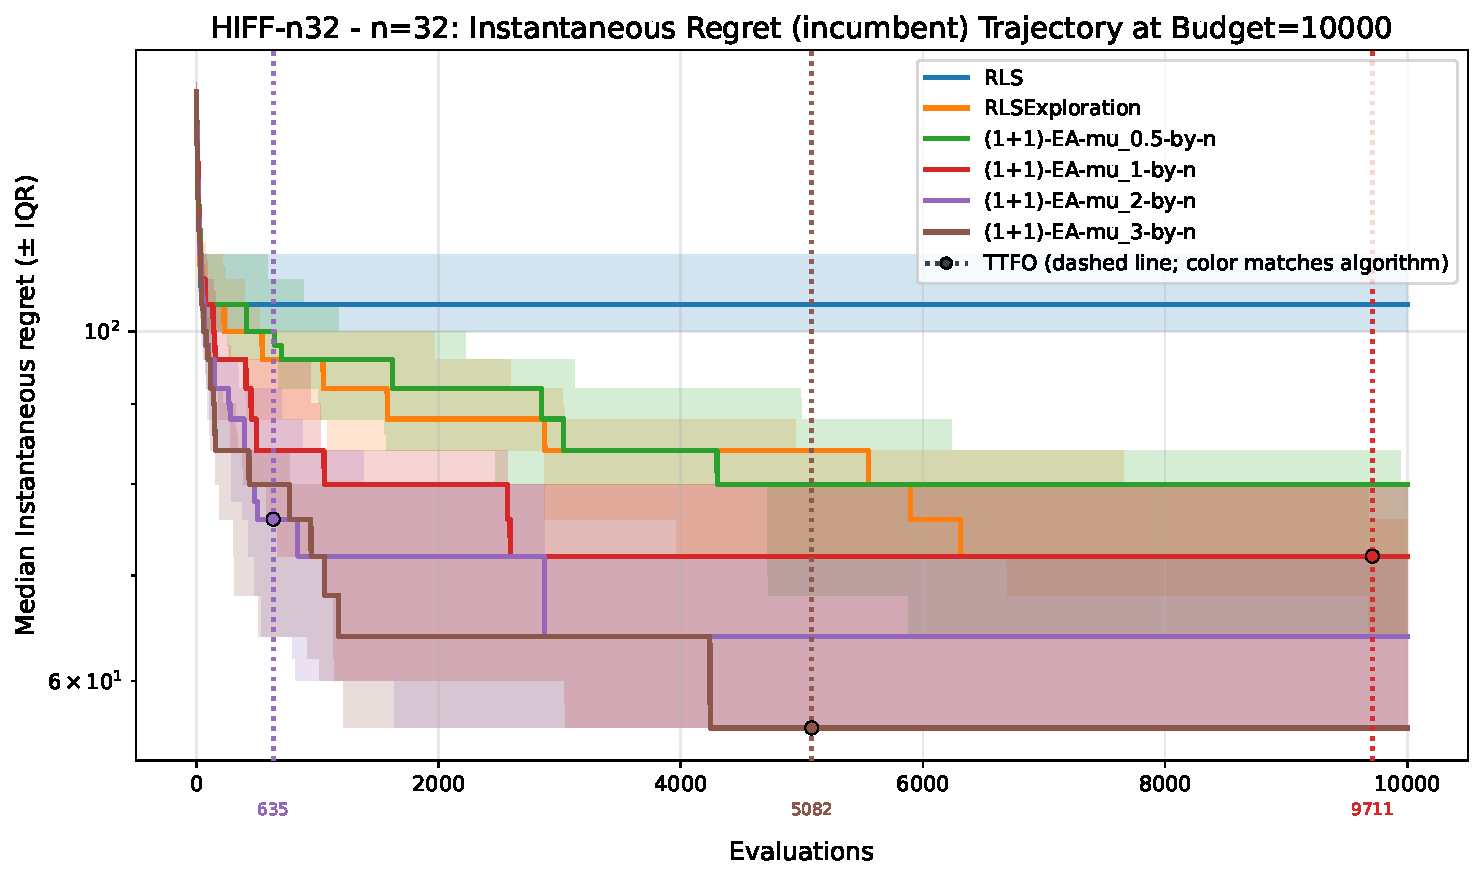
\includegraphics[width=\linewidth]{results/hiff/n32_history_regret_instantaneous_best.pdf}
    \caption{$n=32$ instantaneous regret.}
    \label{fig:suite07-n32-ir}
  \end{subfigure}
  \begin{subfigure}[t]{0.48\textwidth}
    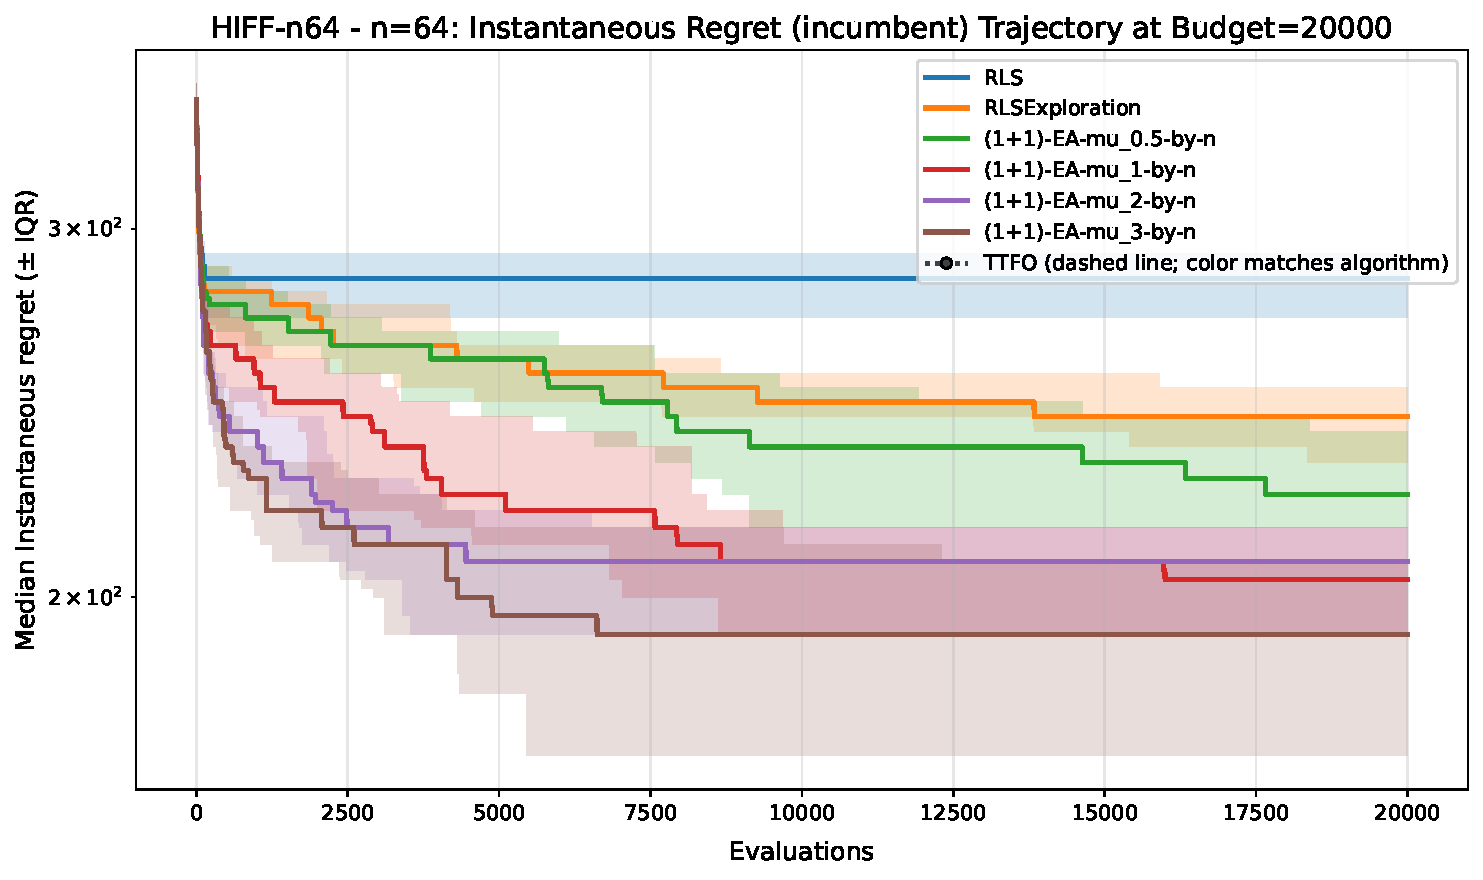
\includegraphics[width=\linewidth]{results/hiff/n64_history_regret_instantaneous_best.pdf}
    \caption{$n=64$ instantaneous regret.}
    \label{fig:suite07-n64-ir}
  \end{subfigure}
  \begin{subfigure}[t]{0.80\textwidth}
    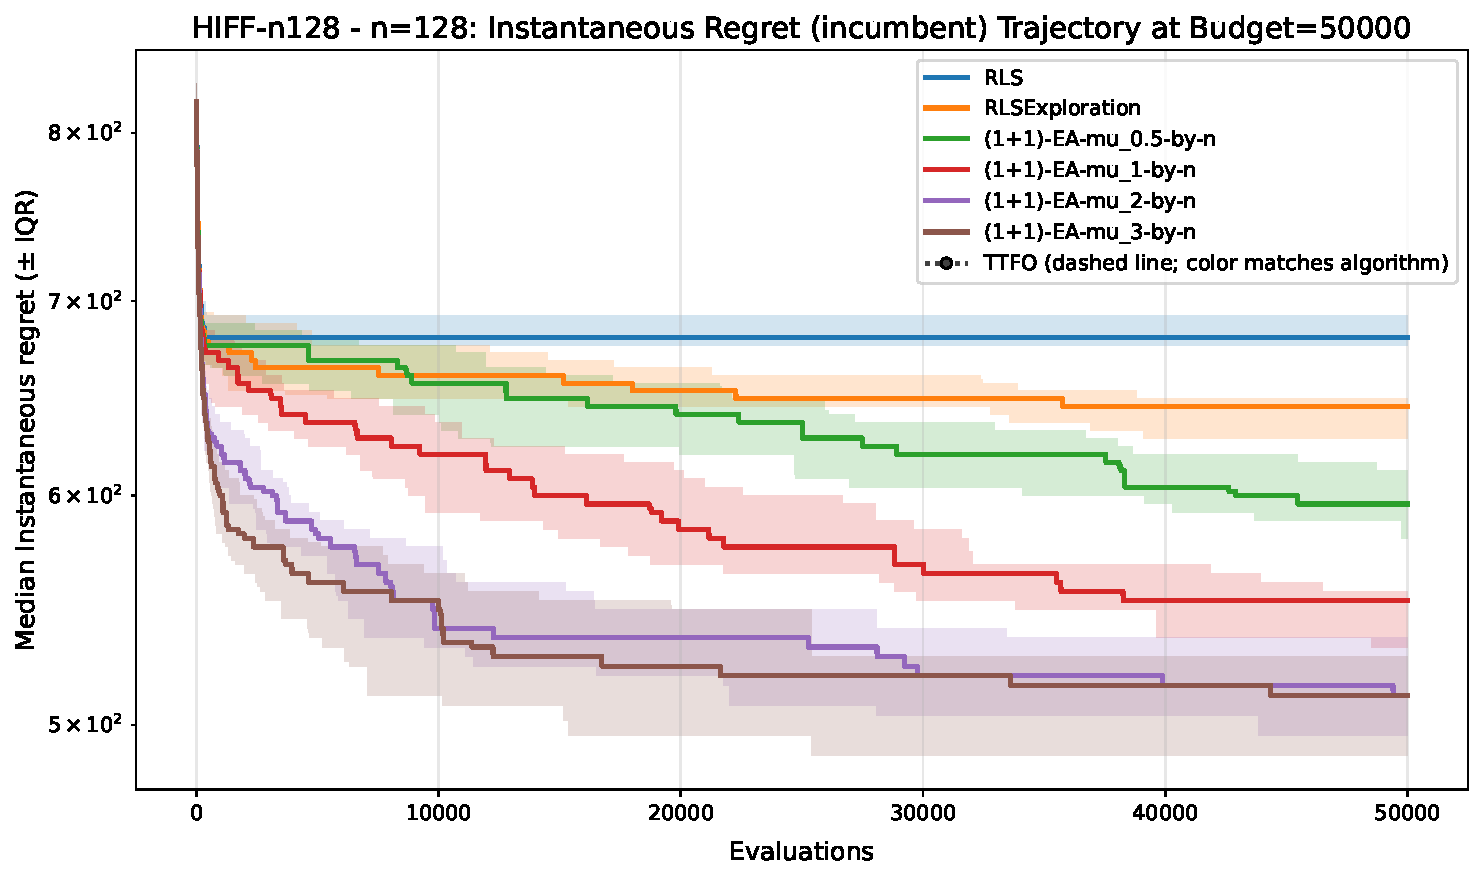
\includegraphics[width=\linewidth]{results/hiff/n128_history_regret_instantaneous_best.pdf}
    \caption{$n=128$ instantaneous regret.}
    \label{fig:suite07-n128-ir}
  \end{subfigure}
  \caption[Suite 07 HIFF instantaneous regret]{Suite~07 incumbent
    \acrshort{ir} trajectories for \acrshort{hiff} as problem size increases.
    The terminal floors show the partial-progress level reached under the
    finite evaluation budgets.}
  \label{fig:suite07-ir}
\end{figure}

\begin{figure}[!htbp]
  \centering
  \begin{subfigure}[t]{0.48\textwidth}
    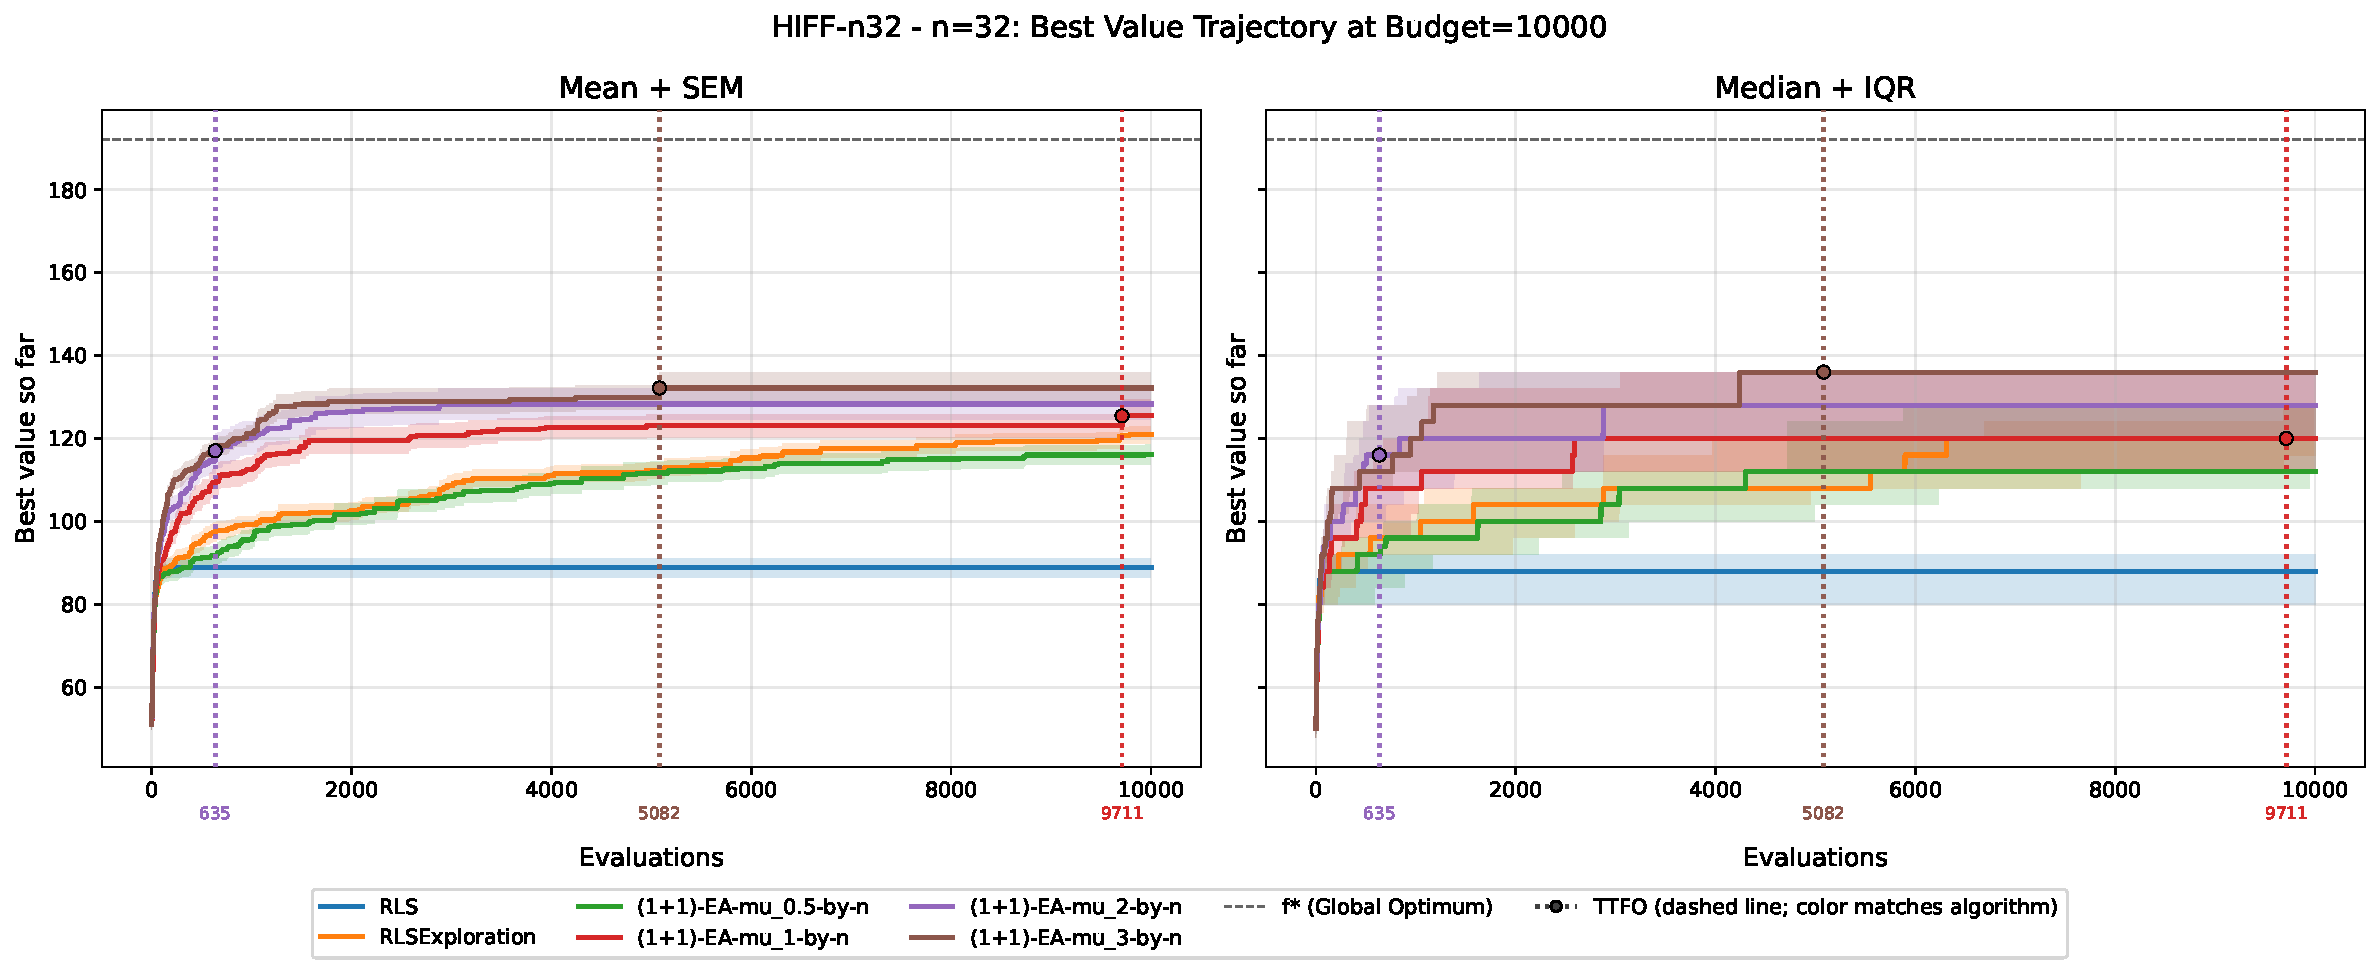
\includegraphics[width=\linewidth]{results/hiff/n32_history_best.pdf}
    \caption{$n=32$ best-so-far fitness.}
    \label{fig:suite07-n32-best}
  \end{subfigure}
  \begin{subfigure}[t]{0.48\textwidth}
    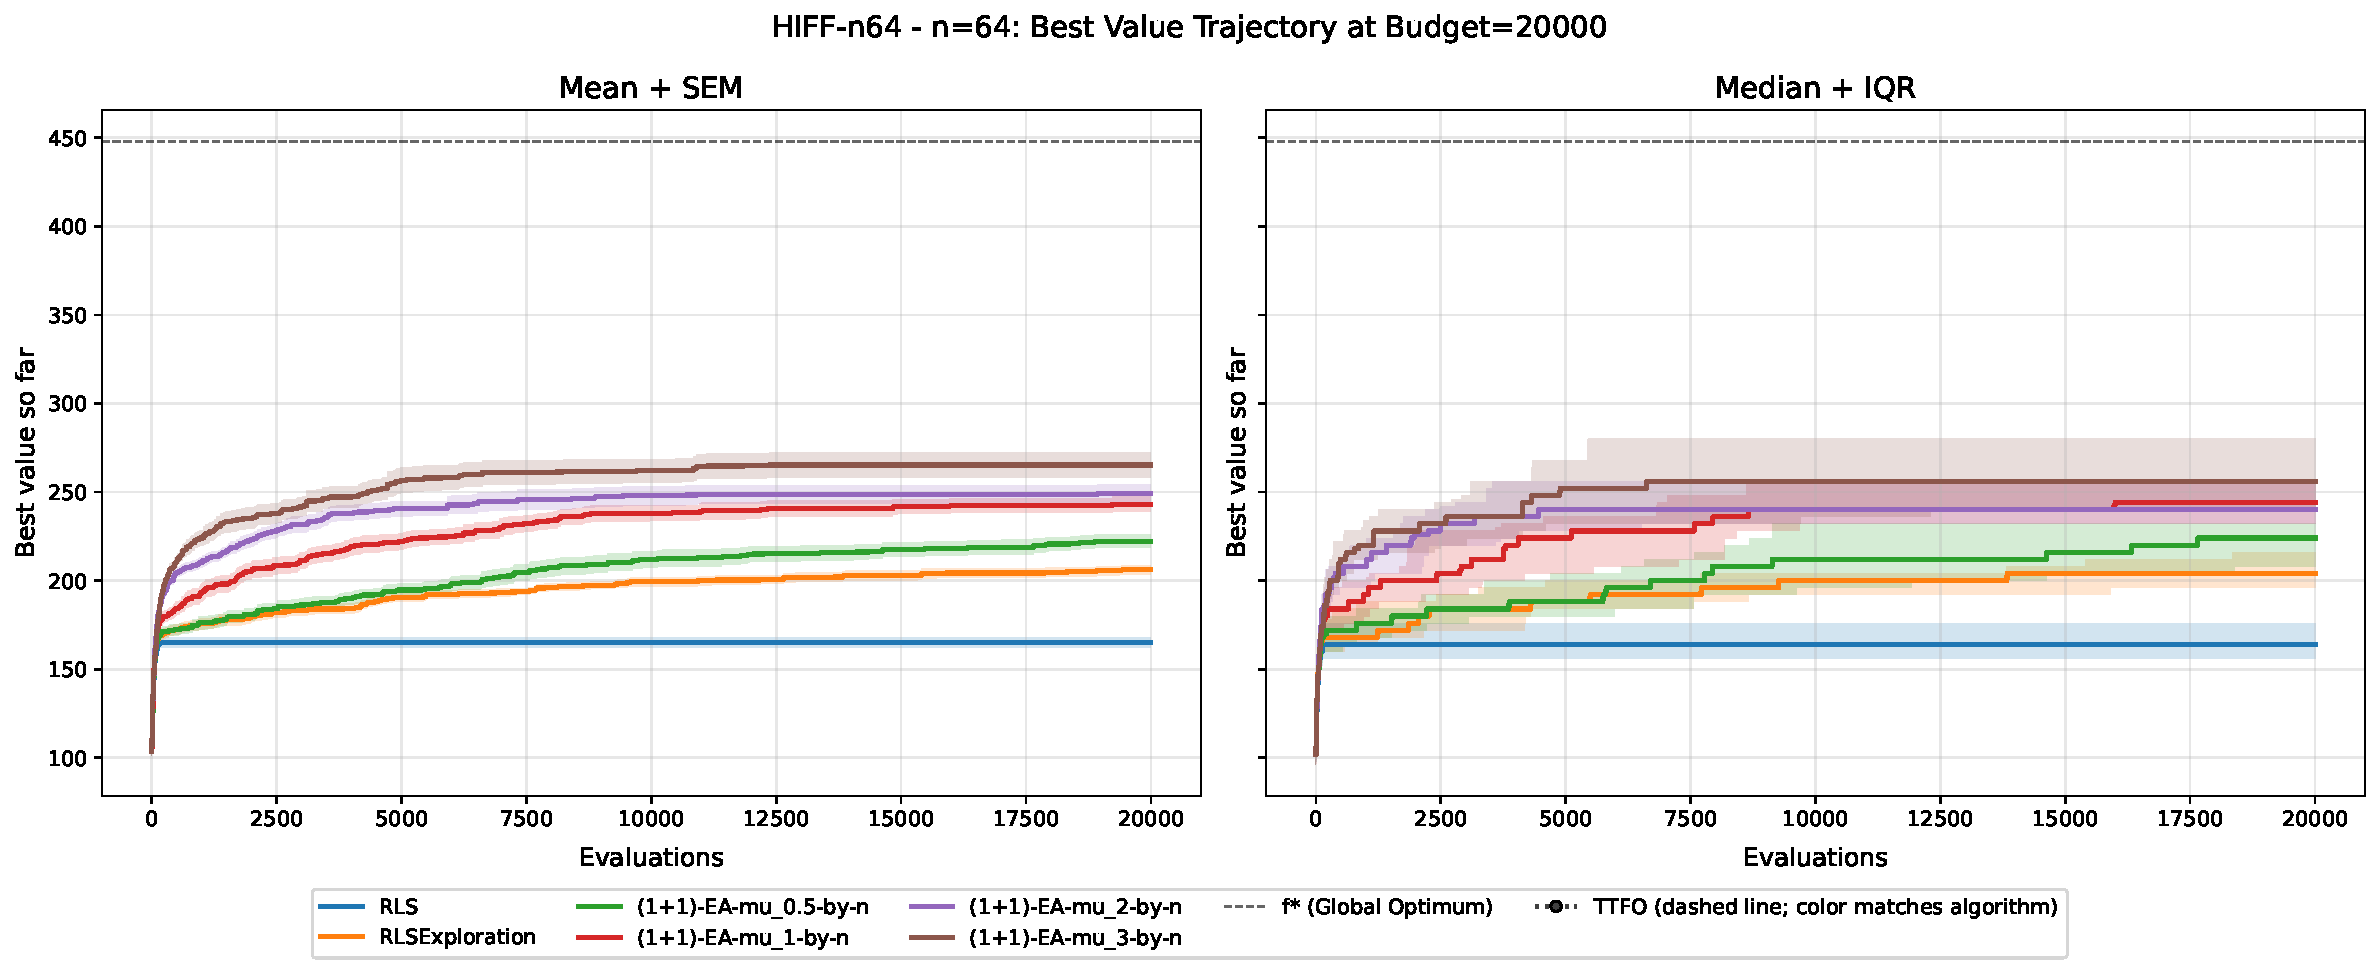
\includegraphics[width=\linewidth]{results/hiff/n64_history_best.pdf}
    \caption{$n=64$ best-so-far fitness.}
    \label{fig:suite07-n64-best}
  \end{subfigure}
  \begin{subfigure}[t]{0.80\textwidth}
    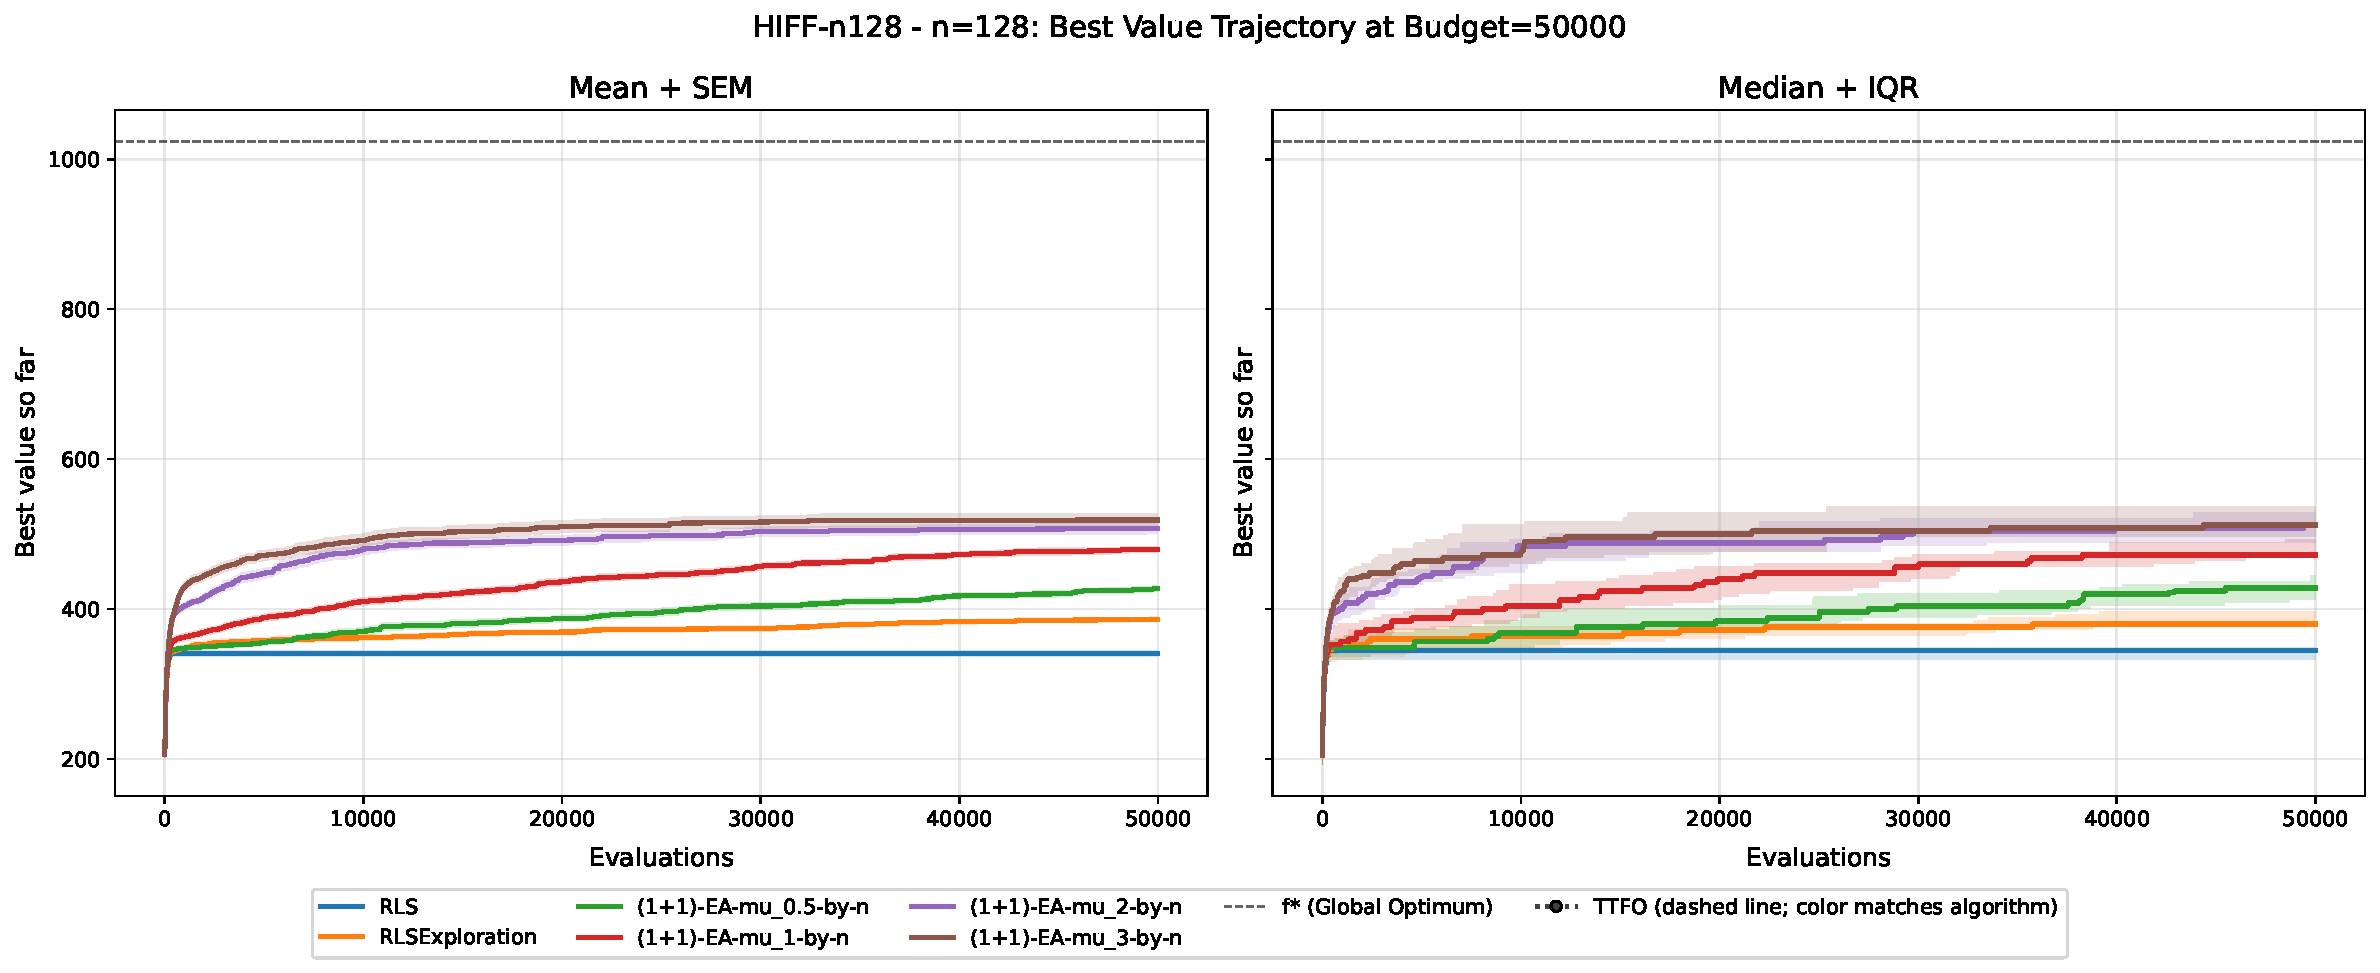
\includegraphics[width=\linewidth]{results/hiff/n128_history_best.pdf}
    \caption{$n=128$ best-so-far fitness.}
    \label{fig:suite07-n128-best}
  \end{subfigure}
  \caption[Suite 07 HIFF best-history plots]{Suite~07 best-so-far fitness
    histories for \acrshort{hiff}. These plots show the hierarchical
    stagnation levels directly, complementing the regret view.}
  \label{fig:suite07-best}
\end{figure}

\begin{figure}[!htbp]
  \centering
  \begin{subfigure}[t]{0.48\textwidth}
    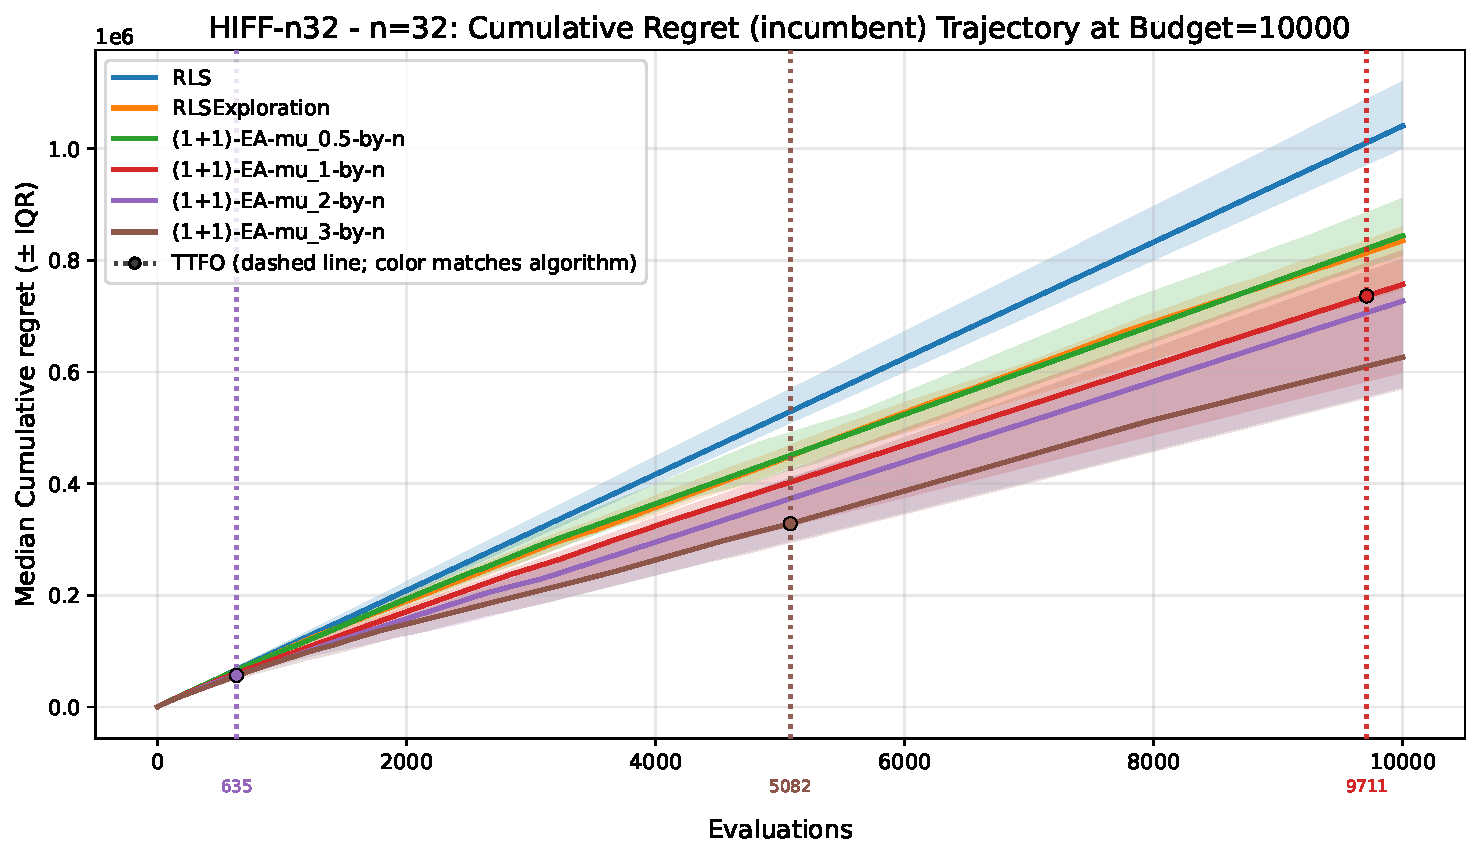
\includegraphics[width=\linewidth]{results/hiff/n32_history_regret_cumulative_best.pdf}
    \caption{$n=32$ cumulative regret.}
    \label{fig:suite07-n32-cr}
  \end{subfigure}
  \begin{subfigure}[t]{0.48\textwidth}
    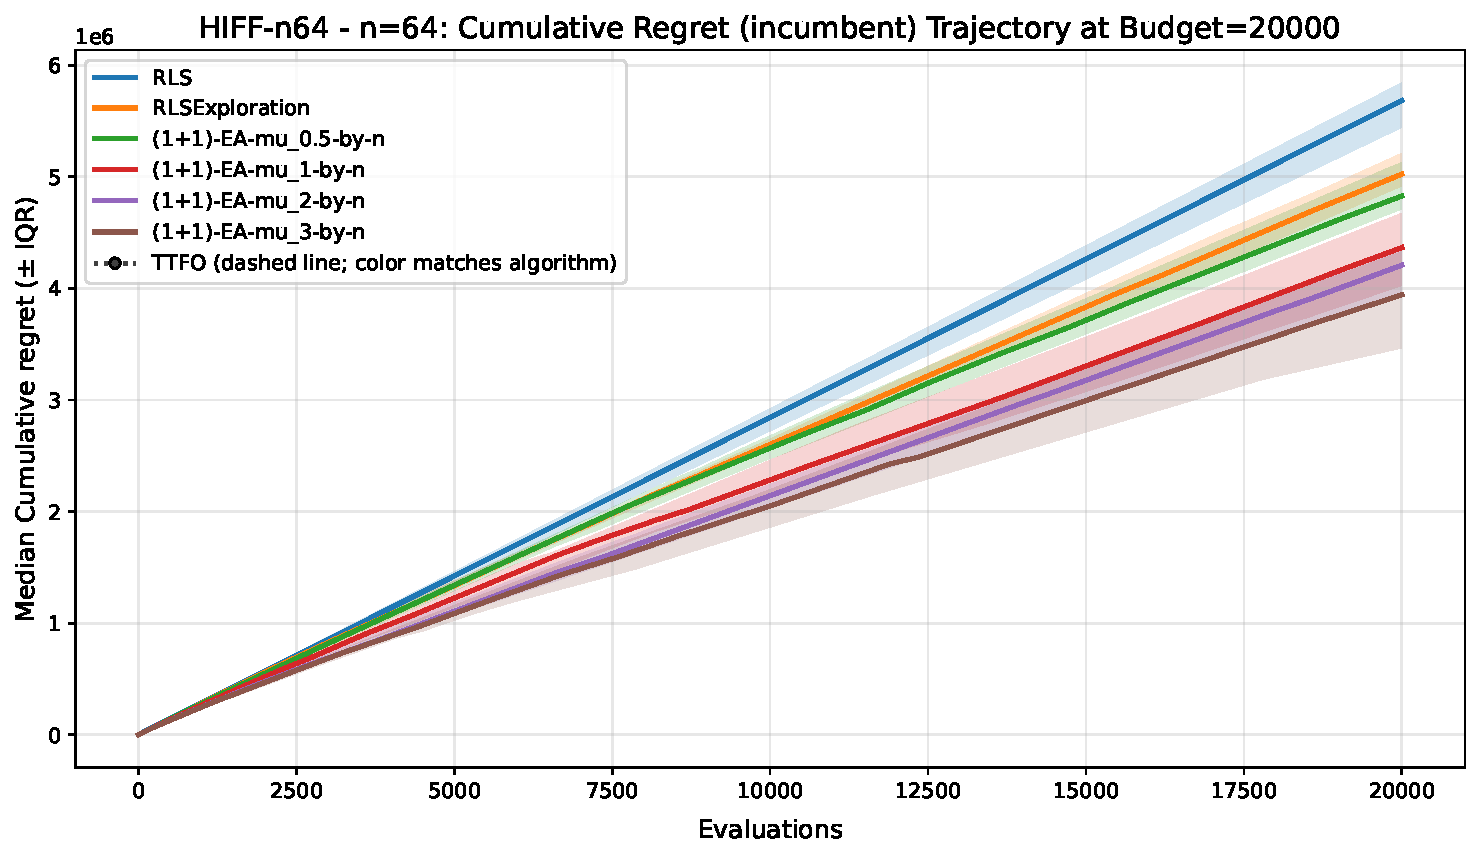
\includegraphics[width=\linewidth]{results/hiff/n64_history_regret_cumulative_best.pdf}
    \caption{$n=64$ cumulative regret.}
    \label{fig:suite07-n64-cr}
  \end{subfigure}
  \begin{subfigure}[t]{0.80\textwidth}
    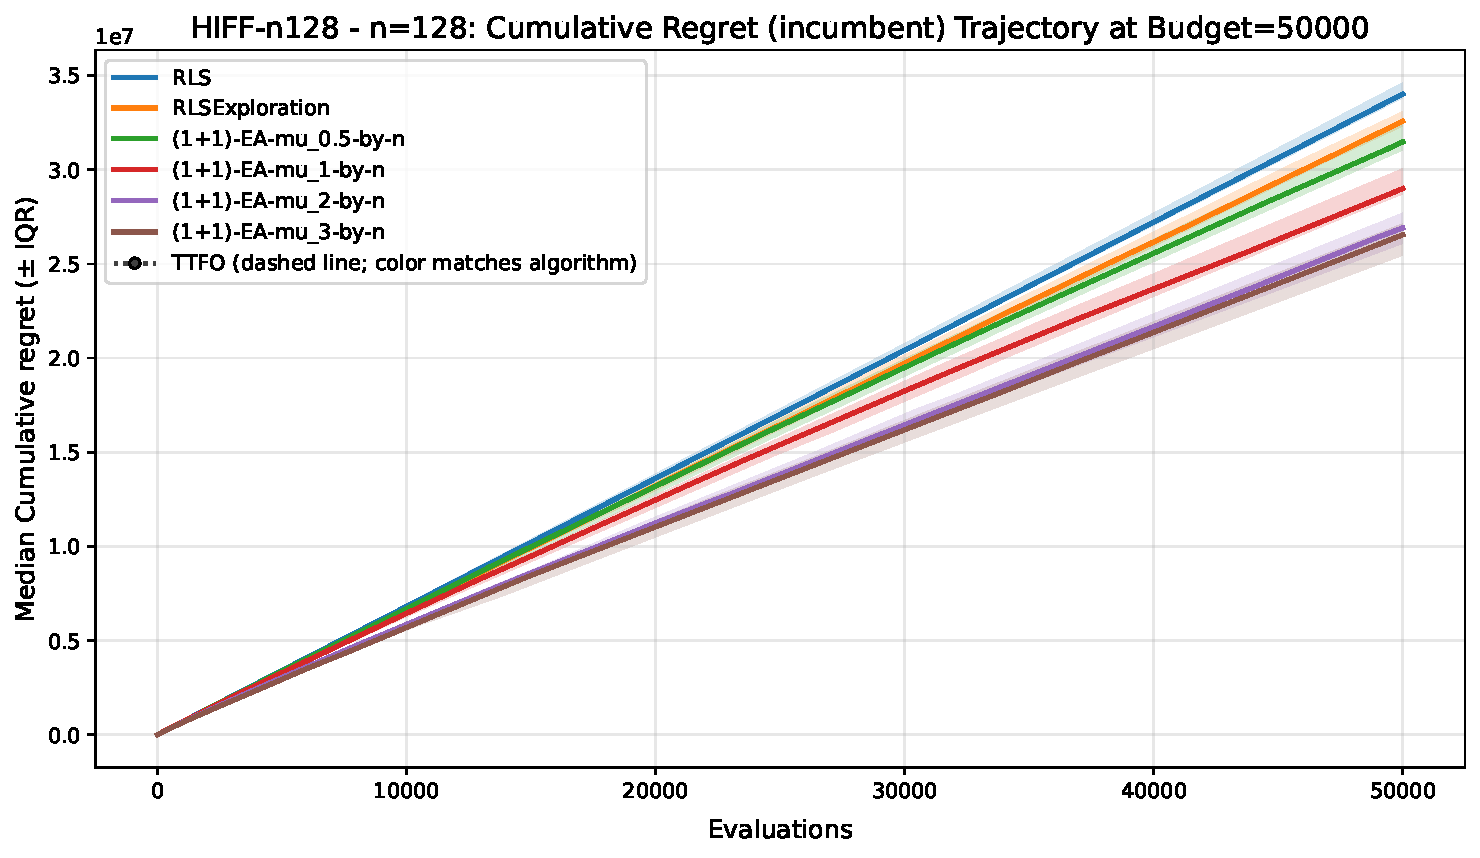
\includegraphics[width=\linewidth]{results/hiff/n128_history_regret_cumulative_best.pdf}
    \caption{$n=128$ cumulative regret.}
    \label{fig:suite07-n128-cr}
  \end{subfigure}
  \caption[Suite 07 HIFF cumulative regret]{Suite~07 incumbent
    \acrshort{cr} trajectories for \acrshort{hiff}. Increasing problem size
    raises the cumulative cost of partial progress under the fixed budgets.}
  \label{fig:suite07-cr}
\end{figure}

Suite~07 should be read as a finite-budget stress test of hierarchical
structure, not as a dedicated asymptotic scaling experiment. Across the tested
problem sizes, $n \in \{32,64,128\}$, the qualitative failure mode is strict
one-bit greediness: once \acrshort{rls} reaches a locally coherent block
structure, improving moves typically require coordinated flips that are
inaccessible to its neighborhood. The resulting \acrshort{ir} floors and
best-fitness stagnation make this failure mode visible before the final budget
(Figures~\ref{fig:suite07-ir} and~\ref{fig:suite07-best}).

The exploratory \acrshort{rlse} variant and the $(1+1)$-\acrshort{ea}
mutation-rate
grid test two ways of relaxing this limitation: accepting occasional worsening
moves, and allowing multi-bit flips. Over the three tested
\acrshort{hiff} sizes,
these mechanisms improve partial progress but do not establish a general
convergence threshold (Figures~\ref{fig:suite07-ir}
and~\ref{fig:suite07-best}). The appropriate conclusion is therefore narrower than a
regret-scaling law: on hierarchical landscapes, mutation and exploration affect
both the final incumbent quality and the rate at which cumulative regret accrues
under a fixed evaluation budget (Figures~\ref{fig:suite07-ir},
\ref{fig:suite07-best}, and~\ref{fig:suite07-cr}).

\section{Cross-Suite Synthesis}
\label{sec:results:synthesis}
%   is never reached within budget --- the condition under which classical
%   measures are least useful and anytime performance measurement matters most.

Across the experimental suites, three takeaways recur. They do not
show that \acrshort{cr} uniquely identifies a landscape class; rather,
they show that the best-so-far regret trajectory records the realized
cost of search under a finite evaluation budget.

\paragraph{Regret discriminates when \acrshort{ttfo} cannot.}
In the hard finite-budget cases, binary convergence measures often go
silent: \textsc{Trap} instances remain non-convergent within budget,
\textsc{Jump} instances with larger $k$ settle onto a width-dependent
regret plateau, and \textsc{Plateau} becomes difficult to distinguish
from \textsc{Jump} once the induced search cost is similar
(Figures~\ref{fig:suite04-trap-cr}, \ref{fig:suite05-jump-cr},
\ref{fig:suite06-plateau-jump-k2}, and~\ref{fig:suite06-plateau-jump-k5}).
High-epistasis NK and larger \acrshort{hiff} instances provide analogous
rugged and hierarchical failure modes rather than literal barrier
landscapes. In all three settings, the slope of incumbent \acrshort{cr},
the floor of incumbent \acrshort{ir}, and the onset of stagnation
continue to describe how far the retained solution remains from the
optimum. This is the operational content of the project's central claim:
regret provides structured information precisely where \acrshort{ttfo}
distributions and $P(\mathrm{opt})$ summaries are least informative.

\paragraph{The asymptotic regret ordering can invert the \acrshort{ttfo} ordering.}
Suites~01 and~02 show that earlier arrival at the global optimum does
not necessarily imply lower cumulative cost. The inversion on
\textsc{LeadingOnes} and \textsc{BinVal}, where \acrshort{rls}
reaches the optimum before the $(1+1)$-\acrshort{ea} but accumulates a
larger regret asymptote, follows the mechanism of
Corollary~\ref{cor:asymptotic-regret}. The asymptote is governed by
first-hitting times across \emph{all} intermediate fitness levels, not
only by the terminal hitting time. Thus, \acrshort{ttfo} records final
arrival, while incumbent cumulative regret records the area under the
best-so-far fitness gap: two algorithms can have the same endpoint, or
even opposite endpoint rankings, while paying different path costs.

\paragraph{Cooling schedule aggressiveness leaves a visible trajectory
signature.}
Suite~11 demonstrates that the \acrshort{ir} curve gives a direct
diagnostic of cooling speed, with the onset of the low-regret floor
ordering schedules from fastest (SA-Exp) to slowest (SA-Log-$d=16$)
(Figure~\ref{fig:suite11-sa-cooling-ir}). Suites~03 and~12 show why this
matters: on low-epistasis NK landscapes, temperature-driven acceptance
inflates cumulative regret relative to hill-climbing baselines, whereas
at high epistasis ($k \geq 6$), calibrated logarithmic cooling maintains
progress after mutation-only methods saturate
(Figures~\ref{fig:suite03-cr} and~\ref{fig:suite12-ir}). The budget at
which SA overtakes the $(1+1)$-\acrshort{ea} on NK-$k=4$ (roughly
$3.3 \times 10^4$ evaluations) is therefore best read as an analog of
the crossover behavior motivating runtime-profile reporting in
\citet{pinto2018practice}, expressed here in the \acrshort{cr} plane
rather than as a literal crossover fitness level.

Suite~08 supports the theoretical interpretation behind these empirical
readings: on integer-valued benchmarks, the profile-derived and directly
averaged \acrshort{cr} curves agree to floating-point precision, consistent with
the tail-sum decomposition of Theorem~\ref{thm:regret-profile}. For real-valued
landscapes such as NK, the profile surfaces should still be read as discretized
approximations, a limitation that bounds but does not invalidate the qualitative
conclusions drawn in Section~\ref{sec:results:nk}. The practical conclusion is that
\acrshort{cr} should be read as a trajectory diagnostic: its slope,
floor, and crossover points expose failure modes that \acrshort{ttfo}
and convergence probability hide under finite budgets.

% Word count aim                3500-4000

% Word count aim: 750-1000
\chapter{Conclusion and Future Work}
\label{cha:conc}

\section{Conclusion}

This project set out to address a gap that \citet{pinto2018practice}
identified explicitly but left open: the absence of a \textit{combined
anytime measure} capable of describing the full quality trajectory of a
black-box optimization algorithm rather than only its terminal behavior.
The three success criteria established in
Section~\ref{subsec:intro:success} provided the evidentiary floor
against which that gap could be declared closed.

\paragraph{Theoretical criterion.}
Theorem~\ref{thm:regret-profile} establishes the required link between
expected incumbent \acrfull{cr} and the distributional runtime profile
$\mathcal{P}(v,t) = \mathbb{P}(\tau_v > t)$. Together with
Corollary~\ref{cor:asymptotic-regret}, it shows that long-run
\acrshort{cr} is governed by expected first-hitting times across
all fitness levels, not only by the time to the optimum. This supplies
the unified anytime measure called for in the literature.

The criterion further required numerical corroboration within
Monte-Carlo sampling error on at least two benchmark functions. Suite
08 (Section~\ref{sec:results:suite08}) provides this corroboration on
\textsc{OneMax} and \textsc{LeadingOnes} for both \acrshort{rls} and
the $(1+1)$-\acrshort{ea}, with scale-normalized maximum pointwise
errors (\acrshort{rmae}) below $1\%$ in all four combinations
(Table~\ref{tab:profile-verification-distances}).
The theoretical criterion is therefore met for the integer-valued benchmark
setting tested here.

\paragraph{Empirical criterion.}
The empirical criterion required \acrshort{cr} trajectories to
yield qualitatively distinct signatures across at least three landscape
archetypes that classical measures cannot separate. The experimental
evidence meets this standard on multiple axes.

On smooth unimodal landscapes (\textsc{OneMax}, \textsc{LeadingOnes},
\textsc{BinVal}), Suites~01 and~02 show that incumbent \acrshort{cr}
curves converge to finite asymptotes whose ordering can \textit{invert}
the \acrshort{ttfo} ordering. Thus, the asymptotic identity has direct
empirical consequence: early progress across intermediate fitness
levels matters, even when the final optimum is eventually reached.

On barrier and deceptive landscapes (\textsc{Jump}, \textsc{Trap},
\textsc{Plateau}), where $P(\text{opt}) \approx 0$ within the
available budget and \acrshort{ttfo} distributions provide no usable
samples, \acrshort{cr} trajectories remain informative. Even when
barrier archetypes are not perfectly separated within the finite
budget, their slopes expose residual fitness gaps and stagnation
levels. This is the operational content of the project's central claim:
regret provides structured information precisely where binary
convergence measures go silent.

SA cooling schedule aggressiveness is directly legible in the
instantaneous regret trajectory (Suite~11), with the onset of the
low-regret floor ordering schedules from fastest to slowest. On NK
landscapes, the regret plots expose the cooling--ruggedness trade-off:
temperature-driven exploration is costly on low-epistasis instances but
becomes competitive, and in calibrated cases beneficial, as epistasis
increases. The empirical criterion is met across more than three
landscape archetypes.

\paragraph{Software criterion.}
The \texttt{regret} framework provides the required reproducible
execution layer for all reported suites, including trajectory
recording, regret computation, runtime-profile analysis, and
\acrfull{ci}-enforced branch coverage across Python 3.12, 3.13, and
3.14.

All three success criteria are therefore satisfied. In answering
\citet{pinto2018practice}'s call, this project demonstrates that
incumbent \acrshort{cr} is a natural extension of fixed-budget
analysis. A connection was established between \acrshort{cr}
and runtime profiles on integer-valued pseudo-Boolean landscapes, with
discretization required beyond that setting.

\section{Future Work}

\paragraph{Tight analytical and asymptotic regret bounds.}
While Theorem~\ref{thm:regret-profile} provides a route from known
hitting-time bounds to regret bounds via the distributional runtime
profile, the resulting expressions are in general loose. Deriving
tight asymptotic characterizations of $\mathbb{E}[\mathrm{CR}(T)]$ for
\acrshort{rls} and the $(1+1)$-\acrshort{ea} on
\textsc{OneMax}, \textsc{LeadingOnes}, and $\textsc{Jump}_k$ remains an
open theoretical problem. A larger scaling study over increasing $n$
would complement this by testing whether observed regret asymptotes
grow at the rates predicted by summing known $\mathbb{E}[\tau_v]$
expressions across fitness levels.

\paragraph{Extension to unknown optima.}
A key assumption throughout this project is that the global optimum
$f^*$ is known in advance, which is necessary for computing exact
regret values. This assumption holds for the emulated benchmark
problems studied here but rarely in genuine black-box practice. Future
work could pursue two complementary directions: the development of
principled heuristics for estimating $f^*$ online, and the adoption of
a probabilistic treatment of the global optimum that would allow the
tail-sum identity to be applied under uncertainty. Problems where the
optimum is known apriori, but the objective landscape remains hidden
represent a particularly tractable intermediate case: the regret
framework developed here provides the necessary foundation for
exploiting that knowledge.

\paragraph{Regret-optimal parameter schedules.}
The $\varepsilon$-greedy and decaying-$\varepsilon$-greedy
\acrshort{rls} variants studied in this project use exploration
schedules motivated by classical bandit theory, but it is not known
whether these schedules minimize \acrshort{cr} in the
pseudo-Boolean setting, where reward structure is non-stationary.
An analog of the UCB1 construction~\cite{auer2002finite} adapted to
the search-space structure of $\{0,1\}^n$ could provide a principled
route to parameter control with explicit regret guarantees, connecting
the exploration--exploitation analysis of online learning to the
adaptive operator selection literature in evolutionary computation.

\paragraph{High-probability tail bounds.}
The analyses presented here concern expected quantities, corresponding
to the Las Vegas framework. Deriving high-probability tail bounds on
incumbent \acrshort{cr}, analogous to the concentration results
available for bandit algorithms~\cite{lattimore2020bandit}, would
allow practitioners to give finite-confidence guarantees on worst-case
trajectory quality rather than only on its expectation.

% Word count aim                0600-750

% Total                         8950-11300

\printbibliography    % this
% causes the references to be listed

%% the bibliography style determines the format  in which both
% citations and references are printed,
%% other possible values are plain and abbrv
%%
%% If you want more control of the format of your citations you might
% want to take a look at
%% natbib.sty, which should be part of any standard LaTeX installation
%%
%% University regulations simply require that your citation style be
% consistent, so see what style
%% your supervisor recommends.

% Appendices start here

%TC:ignore
\appendix

\chapter{Evolutionary Algorithms, Extended}
\label{appendix:ea}

\section[\texorpdfstring{General Form - `$(\mu + \lambda)$-EA'}{General Form - `(mu + lambda)-EA'}]{General Form - `$(\mu + \lambda)$-EA'}
\section{Genetic Algorithms}
\subsection{Crossover}

\section{Parameters \& Operators}
\subsection{Adaptive Mutation \& crossover rates}
\subsection{Selection pressure}


\chapter{Supplementary Optimization Background}

\section{Oracle Tiers: First- and Second-Order Methods}
\label{app:oracle-tiers}

The three tiers of oracle access form an information hierarchy that
governs both the choice and the efficiency of applicable algorithms.

\paragraph{First-Order Methods.}
First-order methods additionally access the gradient
$\nabla f(x) \in \mathbb{R}^d$, which encodes the direction of
steepest ascent at $x$. For a differentiable function
$f : \mathbb{R}^d \to \mathbb{R}$, gradient-based methods exploit
this to define descent directions and form the backbone of classical
continuous optimization~\cite{nocedal2006numerical}. When $f$ is
convex but non-differentiable, the gradient generalizes to the
\textit{subdifferential} $\partial f(x)$, the set of all
\textit{subgradients} $g$ satisfying
\[
  f(y) \geq f(x) + g^\top(y - x) \quad \forall\, y \in \mathbb{R}^d.
\]
Subgradient methods replace the gradient with any element of
$\partial f(x)$, recovering convergence under convexity alone, albeit
at rates slower than those attainable with smooth
gradients~\cite{bertsekas2009convex}.

\paragraph{Second-Order Methods.}
Second-order methods further access the Hessian
$\nabla^2 f(x) \in \mathbb{R}^{d \times d}$, which captures local
curvature. Methods that utilize or approximate the Hessian, such as
Newton and quasi-Newton schemes, can achieve super-linear or quadratic
convergence near a solution~\cite{nocedal2006numerical}, at the cost
of maintaining a $d \times d$ matrix. Together, the three tiers
define distinct levels of oracle access; restricting access
progressively from second-order to zeroth-order culminates in the
black-box model where only function values are observable.

\section{Landscape Properties: Convexity and Smoothness}
\label{app:landscape-props}

\paragraph{Convexity.}
A function $f : \mathbb{R}^d \to \mathbb{R}$ is \textit{convex} if, for all
$x,y \in \mathbb{R}^d$ and $\lambda \in [0,1]$,
\[
  f\!\left(\lambda x + (1-\lambda)y\right)
  \leq \lambda f(x) + (1-\lambda)f(y)
\]
\cite[Def.~1.1.1]{bertsekas2009convex}. For a convex function over a convex
domain, every local minimum is also a global minimum
\cite[Prop.~1.3.2]{bertsekas2009convex}. A differentiable function is
\textit{strongly convex} with parameter $\mu>0$ if
\[
  f(y) \geq f(x) + \nabla f(x)^\top (y-x)
  + \tfrac{\mu}{2}\|y-x\|^2,
\]
which is one of the standard equivalent characterizations of strong convexity
\cite[Thm.~2.1.9]{nesterov2018lectures}. Strong convexity implies a unique
global minimizer \cite[Thm.~2.1.8]{nesterov2018lectures}. Moreover, if $f$
is also $L$-smooth, then gradient descent with a suitable fixed step size
converges linearly \cite[Thm.~2.1.15]{nesterov2018lectures}.

\paragraph{Smoothness and Lipschitz Continuity.}
A differentiable function $f$ is \textit{$L$-smooth} if its gradient
is Lipschitz continuous with constant $L > 0$:
\[
  \|\nabla f(x) - \nabla f(y)\| \leq L\|x - y\|
  \quad \forall\, x, y \in \mathbb{R}^d.
\]
Smoothness bounds the curvature of $f$ from above and is the standard
assumption under which gradient descent achieves an $O(1/T)$
convergence rate for convex objectives~\cite{nocedal2006numerical}.
The objective $f$ itself is \textit{Lipschitz continuous} with
constant $G$ if $|f(x) - f(y)| \leq G\|x - y\|$, a weaker condition
that enables subgradient convergence without differentiability.
Neither property is assumed in the black-box pseudo-Boolean setting
studied in this project.

\section{Haj\'{e}k's Convergence Condition for Simulated Annealing}
\label{app:hajek}

Modelling simulated annealing as a time-inhomogeneous Markov chain
on the state space $\mathcal{X}$, Haj\'{e}k~\cite{hajek1988cooling}
established the following sharp necessary and sufficient condition for
convergence in probability to the global optimum.

\begin{theorem}[Haj\'{e}k 1988]
  Let $d^{*}$ denote the \emph{depth} of the deepest local minimum
  that is not globally optimal, defined as the minimum energy that
  must be crossed to escape it. A cooling schedule $T(t) > 0$
  guarantees that the distribution of the current state converges to
  a distribution supported on the global optima if and only if
  \[
    \sum_{t=1}^{\infty}
    \exp\!\left(\frac{-d^{*}}{T(t)}\right) = +\infty.
  \]
\end{theorem}

For the logarithmic schedule $T(t) = d / \log(t + 1)$, the condition
reduces to the requirement $d \geq d^{*}$: the scaling constant must
be at least as large as the hardest energy barrier in the
landscape~\cite{hajek1988cooling,bertsimas1993simulated}. Logarithmic
cooling is therefore theoretically optimal in the sense that it is
the fastest schedule satisfying the convergence condition.

In practice, $d^{*}$ is unknown for general combinatorial problems,
and logarithmic cooling is often too slow to be useful within a
finite evaluation budget. Exponential cooling
$T(t) = T_0 \cdot \alpha^t$ ($\alpha \in (0,1)$) and linear cooling
$T(t) = \max(T_f,\, T_0 - (T_0 - T_f)\,t/t_{\max})$ cool faster but
violate the condition once the temperature reaches zero, at which
point \acrshort{sa} reduces to a deterministic hill-climber. The
choice of schedule therefore encodes an explicit trade-off between
the convergence guarantee and the practical computational budget.

\section{Plateau Function: Runtime Analysis}
\label{app:plateau-runtime}

\citet{antipov2021precise} establish that for any unbiased mutation
operator the expected runtime of the $(1+1)$-\acrshort{ea} on
\textsc{Plateau}$_k$ is
\[
  \mathbb{E}[T]
  = \frac{n^k}{k!\,\Pr[1 \leq \alpha \leq k]}\,(1 + o(1)),
\]
where $\alpha$ is the number of bits flipped per step. This
expression depends only on the probability of flipping between one
and $k$ bits, not on any other property of the operator. The optimal
mutation rate under standard bit mutation is approximately $k/(en)$,
a factor of $\Theta(k)$ above the canonical $1/n$ recommendation,
mirroring the intuition that wider plateaus require more aggressive
perturbation to exit. This result is directly relevant to the suite
06 and suite 10 experimental analyses, where the contrast between
Jump and Plateau regret trajectories is examined at shared $k$ values.

\chapter{Extended Black-Box Complexity Theory}
\label{app:bbc-extended}

\section{Las Vegas vs.\ Monte Carlo Black-Box Complexity}
\label{app:lv-mc}

In the standard (unrestricted, unbiased) black-box models, the
\textit{Las Vegas} complexity — the expected number of queries until
an optimal solution is first found — and the \textit{Monte Carlo}
complexity — the minimum budget $T$ such that the optimum is found
with probability at least $1 - p$ for a given $p > 0$ — are
essentially equivalent up to constant factors via Markov's inequality:
any Las Vegas algorithm with expected runtime $T$ finds the optimum
within $T/p$ queries with probability at least $1 - p$.

In elitist models, however, this equivalence breaks down severely.
\citet{doerr2015onemax} show that the $(1+1)$ elitist Las Vegas and
Monte Carlo complexities of \textsc{OneMax} can be exponentially far
apart. The reason is structural: an elitist algorithm cannot perform
restarts, because a fresh random starting point will almost surely
have lower fitness than the current incumbent and will therefore be
rejected. Without restarts, a run that fails to find the optimum is
trapped, and there is no mechanism to recover. Consequently, failure
probabilities do not decay geometrically with additional budget in the
same way as for non-elitist algorithms.

Formally, the $p$-\textit{Monte Carlo black-box complexity} of a
problem class $\mathcal{F}$ with respect to an algorithm class
$\mathcal{A}$ is
\[
  \min_{A \in \mathcal{A}}\;
  \min\bigl\{T \in \mathbb{N} :
    \forall f \in \mathcal{F},\;
  \mathbb{P}(\tau_{f^*} \leq T) \geq 1 - p\bigr\}.
\]
The Las Vegas complexity is recovered in the limit by Markov's
inequality when the two notions coincide, but for the $(1+1)$ elitist
Las Vegas complexity of \textsc{OneMax}, \citeauthor{doerr2015onemax}
establish only that it is $O(n \log n)$ (matching the unary unbiased
lower bound) while leaving the exact constant open; the Monte Carlo
complexity is $\Theta(n)$, a separation of a full $\log n$
factor~\cite{doerr2015onemax}.

For the algorithms studied in this project, this distinction does not
affect the experimental results directly: all runtime and regret
analyses use expected quantities over independent runs, which
corresponds to the Las Vegas framework. The Monte Carlo / Las Vegas
distinction becomes relevant if one wishes to derive high-probability
tail bounds on cumulative regret, a direction noted as future work in
Section~\ref{subsec:open-questions}.

\section{Yao's Principle in Restricted Models}
\label{app:yao-restricted}

Yao's Minimax principle in \ref{subsubsec:yaomini} applies directly only to
algorithm classes whose convex hull contains the randomized algorithm
of interest. For memory-restricted and elitist models this containment
fails because some randomized algorithms in these classes are not
convex combinations of deterministic ones. The canonical example is
\acrshort{rls} itself: every deterministic $(1+1)$ memory-restricted
ranking-based algorithm that ever rejects a search point will enter an
infinite loop on \textsc{OneMax} with positive probability when the
input is chosen uniformly at random, giving infinite expected runtime,
whereas \acrshort{rls} optimizes \textsc{OneMax} in $\Theta(n \log n)$
expected queries~\cite{doerr2015onemax}.

\citet{doerr2015onemax} resolve this by applying Yao's principle to
the strictly larger class $\mathcal{A}'$ of all comparison-based
$(1+1)$ algorithms with access to their complete search history.
Every memory-restricted ranking-based algorithm can be simulated in
$\mathcal{A}'$, so a lower bound on the $\mathcal{A}'$-complexity
implies the same lower bound for the original class. The information-
theoretic argument then proceeds as in the unrestricted case: after
$i - 1$ queries the oracle has revealed at most one bit of information
per query, so at most $2^{i-1}$ candidate optima have been eliminated,
giving
\[
  \mathbb{P}(\text{optimum found by query } i) \leq 2^{i - n},
\]
and summing yields $\mathbb{E}[\tau_{f^*}] \geq n - 1$.

\chapter{Related Works}

\subsection{Related Work: Regret in Bayesian and Surrogate-Based Optimization}
\label{subsec:rw-bo-regret}
% - BO is the domain with the most developed regret theory for BBO
% - GP-UCB [Srinivas et al. 2010]: O(sqrt(T gamma_T)) cumulative regret
%   where gamma_T is the information gain, first sublinear regret result
%   for a continuous BBO algorithm
% - Thompson Sampling for BO [Russo & Van Roy, Chowdhury & Srinavas]:
%   Bayesian regret bounds
% - Limitations of BO for the combinatorial setting:
%     GP priors ill-suited to {0,1}^n without kernel engineering
%     Acquisition function optimization is itself an NP-hard BBO problem
%     Poor scaling to large n
% - This motivates studying regret for simpler, combinatorial RSHs

\subsection{Related Work: Regret-Inspired Analysis of Evolutionary Algorithms}
\label{subsec:rw-ea-regret}
% - Fixed-budget / anytime guarantees in EA theory
%   [Jansen & Zarges; Doerr & Doerr - heavy-tailed mutations!CITE!]
% - (1+lambda) EA and population diversity as implicit exploration strategies
% - Algorithms explicitly designed with the exploration-exploitation trade-off
%   in mind: parameter control, self-adaptation, hybrid methods
% - Note: most EA theory is runtime-centric; regret framing is novel here
% - What "regret-aware" EA design might look like:
%     Reward-shaping analogies
%     Budget-sensitive mutation rates
%     Acceptance criteria derived from regret minimization objectives

\subsection{Related Work: Bandit-Inspired Metaheuristics}
\label{subsec:rw-bandit-meta}
% - Algorithm selection / portfolio methods framed as MAB problems
%   [!CITE Fialho, Maturana, Whitley, etc.!]
% - Operator selection in EAs using UCB / EXP3-style rules
%   [adaptive operator selection literature]
% - Hyper-heuristics with bandit-based move selection
% - Common thread: regret minimization used to select operators or algorithms,
%   not to evaluate the optimizer itself - this project does the latter

\chapter{Configuration Schema}
\label{app:schema}

\begin{lstlisting}[language=json,caption={Schema for the configuration files to describe experiments}]
{
  "$schema": "https://json-schema.org/draft/2020-12/schema",
  "type": "object",
  "required": ["suite", "problems", "algorithms", "plotting"],
  "properties": {
    "suite": {
      "type": "object",
      "required": ["name", "runs", "budgets", "mode", "output"],
      "properties": {
        "name": {
          "type": "string",
          "minLength": 1,
          "description": "Name of the experiment suite",
        },
        "description": {
          "type": "string",
          "description": "Optional description of the suite",
        },
        "runs": {
          "type": "integer",
          "minimum": 1,
          "description": "Number of independent runs per configuration",
        },
        "mode": {
          "type": "string",
          "enum": ["lite", "full"],
          "description": "Output mode: 'lite' (stats only) or 'full' (with trajectories)",
        },
        "parallel": {
          "type": "boolean",
          "default": True,
          "description": "Whether to run experiments in parallel (default: true)",
        },
        "profile": {
          "type": "boolean",
          "default": False,
          "description": "Enable runtime profiling analysis outputs (default: false)",
        },
        "budgets": {
          "type": "array",
          "minItems": 1,
          "items": {
            "type": "integer",
            "minimum": 1,
          },
          "description": "List of evaluation budgets to test",
        },
        "output": {
          "type": "object",
          "required": ["raw_root"],
          "properties": {
            "raw_root": {"type": "string"},
            "figures_root": {"type": "string"},
          },
          "additionalProperties": False,
          "description": "Output directory configuration",
        },
      },
      "additionalProperties": False,
    },
    "problems": {
      "type": "array",
      "minItems": 1,
      "items": {
        "type": "object",
        "required": ["name", "class", "params"],
        "properties": {
          "name": {
            "type": "string",
            "minLength": 1,
            "description": "Display name for this configured problem",
          },
          "budget_for_plots": {
            "type": "integer",
            "minimum": 1,
            "description": "Optional per-problem override for budget-specific figures."
            "Default resolution order: problems[i].budget_for_plots -> plotting.budget_for_plots -> max(suite.budgets)",
          },
          "class": {
            "type": "string",
            "minLength": 1,
            "description": "Problem class name from PROBLEM_REGISTRY",
          },
          "params": {
            "type": "object",
            "description": "Problem-specific parameters (e.g., n, k)",
          },
        },
        "additionalProperties": False,
      },
      "description": "List of problem configurations",
    },
    "algorithms": {
      "type": "array",
      "minItems": 1,
      "items": {
        "type": "object",
        "required": ["name", "class", "args"],
        "properties": {
          "name": {
            "type": "string",
            "minLength": 1,
            "description": "Display name for this configured algorithm",
          },
          "class": {
            "type": "string",
            "minLength": 1,
            "description": "Algorithm class name from ALGORITHM_REGISTRY",
          },
          "args": {
            "type": "object",
            "required": ["defaults"],
            "properties": {
              "defaults": {
                "type": "object",
                "description": "Default algorithm parameters",
              },
              "by_problem": {
                "type": "object",
                "default": {},
                "description": "Problem-specific parameter overrides (default: empty mapping)",
              },
            },
            "additionalProperties": False,
            "description": "Algorithm arguments configuration",
          },
        },
        "additionalProperties": False,
      },
      "description": "List of algorithm configurations",
    },
    "plotting": {
      "type": "object",
      "required": ["enabled"],
      "properties": {
        "enabled": {
          "type": "boolean",
          "description": "Master plotting switch (required, no default)",
        },
        "budget_for_plots": {
          "type": "integer",
          "minimum": 1,
          "description": "Budget used for budget-specific figures (defaults to max suite budget)",
        },
        "layout": {
          "type": "object",
          "properties": {
            "per_problem_dir": {
              "type": "boolean",
              "default": True,
              "description": "Create a problem-level subdirectory (default: true)",
            },
            "include_n_subdir": {
              "type": "boolean",
              "default": True,
              "description": "Create an n-size subdirectory (default: true)",
            },
            "structure": {
              "type": "object",
              "properties": {
                "aggregate": {
                  "type": "string",
                  "default": "aggregate",
                  "description": "Subdirectory for cross-budget plots (default: aggregate)",
                },
                "history": {
                  "type": "string",
                  "default": "history",
                  "description": "Subdirectory for trajectory/history plots (default: history)",
                },
                "distribution": {
                  "type": "string",
                  "default": "distributions",
                  "description": "Subdirectory for budget-specific distribution plots (default: distributions)",
                },
                "profile": {
                  "type": "string",
                  "default": "profiles",
                  "description": "Subdirectory for runtime profile plots (default: profiles)",
                },
              },
              "additionalProperties": False,
            },
          },
          "additionalProperties": False,
        },
        "titles": {
          "type": "object",
          "properties": {
            "include_problem_name": {
              "type": "boolean",
              "default": True,
              "description": "Include problem display name in figure titles (default: true)",
            },
            "include_problem_size": {
              "type": "boolean",
              "default": True,
              "description": "Include problem size n in figure titles (default: true)",
            },
          },
          "additionalProperties": False,
        },
        "plots": {
          "type": "object",
          "properties": {
            "regret_curves": {
              "type": "object",
              "properties": {
                "enabled": {
                  "type": "boolean",
                  "default": False,
                  "description": "Enable aggregate regret curve plot (default: false)",
                },
                "filename": {
                  "type": "string",
                  "default": "regret_curves.pdf",
                },
                "log_scale": {
                  "type": "boolean",
                  "default": True,
                  "description": "Use log scaling on budget axis (default: true)",
                },
                "spread": {
                  "type": "string",
                  "enum": [
                    "none",
                    "sem",
                    "sd",
                    "bootstrap_ci",
                    "iqr",
                  ],
                  "default": "sem",
                  "description": "Uncertainty display mode for aggregate regret curves (default: sem)",
                },
                "confidence": {
                  "type": "number",
                  "exclusiveMinimum": 0,
                  "exclusiveMaximum": 1,
                  "default": 0.95,
                },
                "n_bootstrap": {
                  "type": "integer",
                  "minimum": 1,
                  "default": 2000,
                },
                "annotate_pairwise": {
                  "type": "boolean",
                  "default": False,
                },
                "comparison_budget": {
                  "type": "integer",
                  "minimum": 1,
                  "description": "Budget used for pairwise annotation. If omitted, uses the largest available budget",
                },
                "paired_runs": {
                  "type": "boolean",
                  "default": False,
                },
              },
            },
            "convergence_probability": {
              "type": "object",
              "properties": {
                "enabled": {
                  "type": "boolean",
                  "default": False,
                  "description": "Enable convergence probability plot (default: false)",
                },
                "filename": {
                  "type": "string",
                  "default": "convergence_probability.pdf",
                },
                "show_confidence_band": {
                  "type": "boolean",
                  "default": True,
                },
                "confidence": {
                  "type": "number",
                  "exclusiveMinimum": 0,
                  "exclusiveMaximum": 1,
                  "default": 0.95,
                },
              },
            },
            "comparison_heatmap": {
              "type": "object",
              "properties": {
                "enabled": {
                  "type": "boolean",
                  "default": False,
                  "description": "Enable pairwise comparison heatmap (default: false)",
                },
                "filename": {
                  "type": "string",
                  "default": "comparison_heatmap.pdf",
                },
              },
            },
            "regret_boxplots": {
              "type": "object",
              "properties": {
                "enabled": {
                  "type": "boolean",
                  "default": False,
                  "description": "Enable budget-specific regret boxplots (default: false)",
                },
                "filename": {
                  "type": "string",
                  "default": "regret_boxplot_b{budget}.pdf",
                },
                "show_points": {"type": "boolean", "default": True},
                "annotate_pairwise": {
                  "type": "boolean",
                  "default": False,
                },
                "reference_algorithm": {
                  "type": "string",
                  "description": "Reference algorithm for pairwise tests. If omitted and pairwise annotation is enabled, the best mean-regret algorithm at the selected budget is used",
                },
                "paired_runs": {
                  "type": "boolean",
                  "default": False,
                },
              },
            },
            "performance_profile": {
              "type": "object",
              "properties": {
                "enabled": {
                  "type": "boolean",
                  "default": False,
                  "description": "Enable budget-specific performance profiles (default: false)",
                },
                "filename": {
                  "type": "string",
                  "default": "performance_profile_b{budget}.pdf",
                },
                "annotate_pairwise": {
                  "type": "boolean",
                  "default": False,
                },
                "reference_algorithm": {
                  "type": "string",
                  "description": "Reference algorithm for pairwise tests. If omitted and pairwise annotation is enabled, the best mean-regret algorithm at the selected budget is used",
                },
                "paired_runs": {
                  "type": "boolean",
                  "default": False,
                },
              },
            },
            "history_current": {
              "type": "object",
              "properties": {
                "enabled": {
                  "type": "boolean",
                  "default": False,
                  "description": "Enable current-value history trajectory (default: false, requires known f_star)",
                },
                "filename": {
                  "type": "string",
                  "default": "history_current.pdf",
                },
                "series": {
                  "type": "string",
                  "enum": ["current", "best"],
                  "default": "current",
                },
                "log_x": {"type": "boolean", "default": False},
                "log_y": {"type": "boolean", "default": False},
                "show_ttfo_markers": {
                  "type": "boolean",
                  "default": True,
                },
                "spread": {
                  "type": "string",
                  "enum": [
                    "none",
                    "sem",
                    "sd",
                    "bootstrap_ci",
                    "iqr",
                  ],
                  "default": "sem",
                },
                "confidence": {
                  "type": "number",
                  "exclusiveMinimum": 0,
                  "exclusiveMaximum": 1,
                  "default": 0.95,
                },
                "n_bootstrap": {
                  "type": "integer",
                  "minimum": 1,
                  "default": 1000,
                },
              },
            },
            "history_best": {
              "type": "object",
              "properties": {
                "enabled": {
                  "type": "boolean",
                  "default": False,
                  "description": "Enable best-value history trajectory (default: false, requires known f_star)",
                },
                "filename": {
                  "type": "string",
                  "default": "history_best.pdf",
                },
                "series": {
                  "type": "string",
                  "enum": ["current", "best"],
                  "default": "best",
                },
                "log_x": {"type": "boolean", "default": False},
                "log_y": {"type": "boolean", "default": False},
                "show_ttfo_markers": {
                  "type": "boolean",
                  "default": True,
                },
                "spread": {
                  "type": "string",
                  "enum": [
                    "none",
                    "sem",
                    "sd",
                    "bootstrap_ci",
                    "iqr",
                  ],
                  "default": "sem",
                },
                "confidence": {
                  "type": "number",
                  "exclusiveMinimum": 0,
                  "exclusiveMaximum": 1,
                  "default": 0.95,
                },
                "n_bootstrap": {
                  "type": "integer",
                  "minimum": 1,
                  "default": 1000,
                },
              },
            },
            "regret_instantaneous": {
              "type": "object",
              "properties": {
                "enabled": {
                  "type": "boolean",
                  "default": False,
                  "description": "Enable instantaneous regret trajectory (default: false, requires known f_star)",
                },
                "filename": {
                  "type": "string",
                  "default": "history_regret_instantaneous.pdf",
                },
                "series": {
                  "type": "string",
                  "enum": ["instantaneous", "cumulative"],
                  "default": "instantaneous",
                },
                "track_incumbent": {
                  "type": "boolean",
                  "default": False,
                },
                "log_x": {"type": "boolean", "default": False},
                "log_y": {"type": "boolean", "default": True},
                "show_ttfo_markers": {
                  "type": "boolean",
                  "default": True,
                },
                "spread": {
                  "type": "string",
                  "enum": [
                    "none",
                    "sem",
                    "sd",
                    "bootstrap_ci",
                    "iqr",
                  ],
                  "default": "sem",
                },
                "confidence": {
                  "type": "number",
                  "exclusiveMinimum": 0,
                  "exclusiveMaximum": 1,
                  "default": 0.95,
                },
                "n_bootstrap": {
                  "type": "integer",
                  "minimum": 1,
                  "default": 1000,
                },
              },
            },
            "regret_cumulative": {
              "type": "object",
              "properties": {
                "enabled": {
                  "type": "boolean",
                  "default": False,
                  "description": "Enable cumulative regret trajectory (default: false, requires known f_star)",
                },
                "filename": {
                  "type": "string",
                  "default": "history_regret_cumulative.pdf",
                },
                "series": {
                  "type": "string",
                  "enum": ["instantaneous", "cumulative"],
                  "default": "cumulative",
                },
                "track_incumbent": {
                  "type": "boolean",
                  "default": False,
                },
                "log_x": {"type": "boolean", "default": False},
                "log_y": {"type": "boolean", "default": False},
                "show_ttfo_markers": {
                  "type": "boolean",
                  "default": True,
                },
                "spread": {
                  "type": "string",
                  "enum": [
                    "none",
                    "sem",
                    "sd",
                    "bootstrap_ci",
                    "iqr",
                  ],
                  "default": "sem",
                },
                "confidence": {
                  "type": "number",
                  "exclusiveMinimum": 0,
                  "exclusiveMaximum": 1,
                  "default": 0.95,
                },
                "n_bootstrap": {
                  "type": "integer",
                  "minimum": 1,
                  "default": 1000,
                },
              },
            },
            "regret_instantaneous_best": {
              "type": "object",
              "properties": {
                "enabled": {
                  "type": "boolean",
                  "default": False,
                  "description": "Enable instantaneous regret over best-so-far values (default: false, requires known f_star)",
                },
                "filename": {
                  "type": "string",
                  "default": "history_regret_instantaneous_best.pdf",
                },
                "series": {
                  "type": "string",
                  "enum": ["instantaneous", "cumulative"],
                  "default": "instantaneous",
                },
                "track_incumbent": {"type": "boolean", "default": True},
                "log_x": {"type": "boolean", "default": False},
                "log_y": {"type": "boolean", "default": True},
                "show_ttfo_markers": {
                  "type": "boolean",
                  "default": True,
                },
                "spread": {
                  "type": "string",
                  "enum": [
                    "none",
                    "sem",
                    "sd",
                    "bootstrap_ci",
                    "iqr",
                  ],
                  "default": "sem",
                },
                "confidence": {
                  "type": "number",
                  "exclusiveMinimum": 0,
                  "exclusiveMaximum": 1,
                  "default": 0.95,
                },
                "n_bootstrap": {
                  "type": "integer",
                  "minimum": 1,
                  "default": 1000,
                },
              },
            },
            "regret_cumulative_best": {
              "type": "object",
              "properties": {
                "enabled": {
                  "type": "boolean",
                  "default": False,
                  "description": "Enable cumulative regret over best-so-far values (default: false, requires known f_star)",
                },
                "filename": {
                  "type": "string",
                  "default": "history_regret_cumulative_best.pdf",
                },
                "series": {
                  "type": "string",
                  "enum": ["instantaneous", "cumulative"],
                  "default": "cumulative",
                },
                "track_incumbent": {"type": "boolean", "default": True},
                "log_x": {"type": "boolean", "default": False},
                "log_y": {"type": "boolean", "default": False},
                "show_ttfo_markers": {
                  "type": "boolean",
                  "default": True,
                },
                "spread": {
                  "type": "string",
                  "enum": [
                    "none",
                    "sem",
                    "sd",
                    "bootstrap_ci",
                    "iqr",
                  ],
                  "default": "sem",
                },
                "confidence": {
                  "type": "number",
                  "exclusiveMinimum": 0,
                  "exclusiveMaximum": 1,
                  "default": 0.95,
                },
                "n_bootstrap": {
                  "type": "integer",
                  "minimum": 1,
                  "default": 1000,
                },
              },
            },
            "ttfo_distribution": {
              "type": "object",
              "properties": {
                "enabled": {
                  "type": "boolean",
                  "default": False,
                  "description": "Enable TTFO distribution plot (default: false)",
                },
                "filename": {
                  "type": "string",
                  "default": "history_ttfo_markers.pdf",
                },
                "tolerance": {
                  "type": "number",
                  "minimum": 0,
                  "default": 1e-9,
                },
                "show_median": {
                  "type": "boolean",
                  "default": True,
                },
                "annotate_pairwise": {
                  "type": "boolean",
                  "default": False,
                },
                "reference_algorithm": {
                  "type": "string",
                  "description": "Reference algorithm for pairwise tests. If omitted and pairwise annotation is enabled, the algorithm with the lowest mean TTFO is used",
                },
                "paired_runs": {
                  "type": "boolean",
                  "default": False,
                },
              },
            },
            "inverse_runtime_profile_surface": {
              "type": "object",
              "properties": {
                "enabled": {
                  "type": "boolean",
                  "default": False,
                  "description": "Enable per-algorithm inverse runtime profile surface plot (default: false, requires suite.profile=true)",
                },
                "filename": {
                  "type": "string",
                  "default": "inverse_runtime_profile_surface_{algorithm}.pdf",
                  "description": "Include `{algorithm}` as a placeholder in the filename",
                },
              },
            },
            "inverse_runtime_profile_curves": {
              "type": "object",
              "properties": {
                "enabled": {
                  "type": "boolean",
                  "default": False,
                  "description": "Enable inverse runtime profile curve plot (default: false, requires suite.profile=true)",
                },
                "filename": {
                  "type": "string",
                  "default": "inverse_runtime_profile_curves.pdf",
                },
              },
            },
            "cr_profile_verification": {
              "type": "object",
              "properties": {
                "enabled": {
                  "type": "boolean",
                  "default": False,
                  "description": "Enable profile identity verification plot (default: false, requires suite.profile=true)",
                },
                "filename": {
                  "type": "string",
                  "default": "cr_profile_verification.pdf",
                },
              },
            },
          },
          "additionalProperties": False,
        },
      },
      "additionalProperties": False,
      "description": "Plotting configuration",
    },
  },
  "allOf": [
    {
      "if": {
        "properties": {
          "plotting": {
            "type": "object",
            "properties": {
              "enabled": {"const": True},
            },
            "required": ["enabled"],
          }
        }
      },
      "then": {
        "properties": {
          "suite": {
            "type": "object",
            "properties": {
              "output": {
                "type": "object",
                "required": ["figures_root"],
              }
            },
          }
        }
      },
    },
    {
      "if": {
        "properties": {
          "suite": {
            "type": "object",
            "properties": {
              "profile": {"const": False},
            },
          }
        }
      },
      "then": {
        "properties": {
          "plotting": {
            "type": "object",
            "properties": {
              "plots": {
                "type": "object",
                "properties": {
                  "inverse_runtime_profile_surface": {
                    "type": "object",
                    "properties": {
                      "enabled": {"const": False},
                    },
                  },
                  "inverse_runtime_profile_curves": {
                    "type": "object",
                    "properties": {
                      "enabled": {"const": False},
                    },
                  },
                  "cr_profile_verification": {
                    "type": "object",
                    "properties": {
                      "enabled": {"const": False},
                    },
                  },
                },
              }
            },
          }
        }
      },
    },
  ],
  "additionalProperties": False,
}
\end{lstlisting}

%TC:endignore

\end{document}
